% This must be in the first 5 lines to tell arXiv to use pdfLaTeX, which is strongly recommended.
\pdfoutput=1
% In particular, the hyperref package requires pdfLaTeX in order to break URLs across lines.

\documentclass[11pt]{article}

% Remove the "review" option to generate the final version.
\usepackage{ACL2023}

% Standard package includes
\usepackage{times}
\usepackage{latexsym}
\usepackage{booktabs} % Added for \toprule, \midrule, and \bottomrule
\usepackage{amsmath} % Added for \tfrac and other math commands
\usepackage{amssymb} % Added for \mathbb and additional math symbols
\usepackage{adjustbox}
% For proper rendering and hyphenation of words containing Latin characters (including in bib files)
\usepackage[T1]{fontenc}
% For Vietnamese characters
% \usepackage[T5]{fontenc}
% See https://www.latex-project.org/help/documentation/encguide.pdf for other character sets
\usepackage{wrapfig}

\graphicspath{{../graphs/}{graphs/}} % Search in repo graphs/ from paper dir

% This assumes your files are encoded as UTF8
\usepackage[utf8]{inputenc}

% This is not strictly necessary, and may be commented out.
% However, it will improve the layout of the manuscript,
% and will typically save some space.
\usepackage{microtype}

\usepackage{inconsolata}

\usepackage{graphicx}
\usepackage{hyperref}
\usepackage{mathtools}
\usepackage{parskip}
\usepackage{pgfplots}
\usepackage{placeins}
\usepackage{layouts}
\usepackage{multirow}


% If the title and author information does not fit in the area allocated, uncomment the following
%
%\setlength\titlebox{<dim>}
%
% and set <dim> to something 5cm or larger.

\title{SampledKD: Two-Axis Selection for Efficient Distillation}
% \title{SampledKD: Extreme Sampling, Near Full Distillation Accuracy}
% \title{SampledKD: How Extreme Can Sampling Be While Matching Accuracy?}
% \title{SampledKD: How Efficient Could Distillation Get While Match Accuracy?}
% \title{SampledKD: Could Distillation be So Much More Efficient?}

% Author information can be set in various styles:
% For several authors from the same institution:
% \author{Author 1 \and ... \and Author n \\
%         Address line \\ ... \\ Address line}
% if the names do not fit well on one line use
%         Author 1 \\ {\bf Author 2} \\ ... \\ {\bf Author n} \\
% For authors from different institutions:
% \author{Author 1 \\ Address line \\  ... \\ Address line
%         \And  ... \And
%         Author n \\ Address line \\ ... \\ Address line}
% To start a separate ``row'' of authors use \AND, as in
% \author{Author 1 \\ Address line \\  ... \\ Address line
%         \AND
%         Author 2 \\ Address line \\ ... \\ Address line \And
%         Author 3 \\ Address line \\ ... \\ Address line}

\author{
  Almog Tavor\textsuperscript{*} \qquad Itay Ebenspanger\textsuperscript{*} \qquad Neil Cnaan\textsuperscript{*} \\
  Blavatnik School of Computer Science and AI \\
  Tel Aviv University \\
  \texttt{\{almogt, ebenspanger, neilcnaan\}@mail.tau.ac.il} \\
}

\begin{document}
\maketitle
\let\thefootnote\relax
\footnotemark
\footnotetext{* Equal contribution.}
\footnotetext{\url{https://github.com/almogtavor/sampled-knowledge-distillation}}
\begin{abstract}
	Knowledge distillation (KD) compresses LLMs but often requires storing or querying full teacher logits and supervising every token.
	We revisit where and how to distill.
	First, we propose token-selective KD (TSKD), which selects informative positions (by teacher entropy, teacher-student KL, or student loss) and applies standard KL divergence there, leaving other positions to cross-entropy only.
	Second, SampledKD adds logits-level random sampling, so the expected KD gradient matches full KD while caching only a few teacher classes per position.
	On our small-scale setting, TSKD improves over FullKD on several benchmarks at similar compute, while SampledKD substantially reduces logit storage with a modest accuracy gap that we hypothesize can shrink at larger scales.
	We release code for reproduction.
\end{abstract}

\section{Introduction}

Large language models (LLMs) achieve state-of-the-art results across diverse tasks, but their size makes them expensive to serve and difficult to adapt.
Recent work shows that a small fraction of high-entropy "forking" tokens disproportionately drives learning in reinforcement learning from reasoning tasks \citep{wang2025highentropy}, suggesting that selective supervision may yield better efficiency-accuracy trade-offs.
Motivated by this insight, we study knowledge distillation (KD), a standard approach that compresses LLMs by training a smaller student model to imitate a larger teacher \citep{hinton2015distillation}, and ask whether focusing KD on these high-entropy tokens can deliver more efficient distillation without sacrificing performance.

\begin{figure}[t!]
	\begin{flushright}
		\resizebox{\columnwidth}{!}{%% Creator: Matplotlib, PGF backend
%%
%% To include the figure in your LaTeX document, write
%%   \input{<filename>.pgf}
%%
%% Make sure the required packages are loaded in your preamble
%%   \usepackage{pgf}
%%
%% Also ensure that all the required font packages are loaded; for instance,
%% the lmodern package is sometimes necessary when using math font.
%%   \usepackage{lmodern}
%%
%% Figures using additional raster images can only be included by \input if
%% they are in the same directory as the main LaTeX file. For loading figures
%% from other directories you can use the `import` package
%%   \usepackage{import}
%%
%% and then include the figures with
%%   \import{<path to file>}{<filename>.pgf}
%%
%% Matplotlib used the following preamble
%%   \def\mathdefault#1{#1}
%%   \everymath=\expandafter{\the\everymath\displaystyle}
%%   \IfFileExists{scrextend.sty}{
%%     \usepackage[fontsize=10.000000pt]{scrextend}
%%   }{
%%     \renewcommand{\normalsize}{\fontsize{10.000000}{12.000000}\selectfont}
%%     \normalsize
%%   }
%%   
%%   \makeatletter\@ifpackageloaded{underscore}{}{\usepackage[strings]{underscore}}\makeatother
%%
\begingroup%
\makeatletter%
\begin{pgfpicture}%
\pgfpathrectangle{\pgfpointorigin}{\pgfqpoint{10.062297in}{7.290000in}}%
\pgfusepath{use as bounding box, clip}%
\begin{pgfscope}%
\pgfsetbuttcap%
\pgfsetmiterjoin%
\definecolor{currentfill}{rgb}{1.000000,1.000000,1.000000}%
\pgfsetfillcolor{currentfill}%
\pgfsetlinewidth{0.000000pt}%
\definecolor{currentstroke}{rgb}{1.000000,1.000000,1.000000}%
\pgfsetstrokecolor{currentstroke}%
\pgfsetdash{}{0pt}%
\pgfpathmoveto{\pgfqpoint{0.000000in}{0.000000in}}%
\pgfpathlineto{\pgfqpoint{10.062297in}{0.000000in}}%
\pgfpathlineto{\pgfqpoint{10.062297in}{7.290000in}}%
\pgfpathlineto{\pgfqpoint{0.000000in}{7.290000in}}%
\pgfpathlineto{\pgfqpoint{0.000000in}{0.000000in}}%
\pgfpathclose%
\pgfusepath{fill}%
\end{pgfscope}%
\begin{pgfscope}%
\definecolor{textcolor}{rgb}{0.000000,0.000000,0.000000}%
\pgfsetstrokecolor{textcolor}%
\pgfsetfillcolor{textcolor}%
\pgftext[x=1.424632in,y=7.110000in,,]{\color{textcolor}{\rmfamily\fontsize{28.000000}{38.400000}\bfseries\selectfont\catcode`\^=\active\def^{\ifmmode\sp\else\^{}\fi}\catcode`\%=\active\def%{\%}FullKD}}%
\end{pgfscope}%
\begin{pgfscope}%
\definecolor{textcolor}{rgb}{0.000000,0.000000,0.000000}%
\pgfsetstrokecolor{textcolor}%
\pgfsetfillcolor{textcolor}%
\pgftext[x=4.843750in,y=7.110000in,,]{\color{textcolor}{\rmfamily\fontsize{28.000000}{38.400000}\bfseries\selectfont\catcode`\^=\active\def^{\ifmmode\sp\else\^{}\fi}\catcode`\%=\active\def%{\%}RS-KD}}%
\end{pgfscope}%
\begin{pgfscope}%
\definecolor{textcolor}{rgb}{0.000000,0.000000,0.000000}%
\pgfsetstrokecolor{textcolor}%
\pgfsetfillcolor{textcolor}%
\pgftext[x=8.262868in,y=7.110000in,,]{\color{textcolor}{\rmfamily\fontsize{28.000000}{38.400000}\bfseries\selectfont\catcode`\^=\active\def^{\ifmmode\sp\else\^{}\fi}\catcode`\%=\active\def%{\%}Ours (2-axis RS-KD)}}%
\end{pgfscope}%
\begin{pgfscope}%
\pgfsetbuttcap%
\pgfsetmiterjoin%
\definecolor{currentfill}{rgb}{1.000000,1.000000,1.000000}%
\pgfsetfillcolor{currentfill}%
\pgfsetlinewidth{0.000000pt}%
\definecolor{currentstroke}{rgb}{0.000000,0.000000,0.000000}%
\pgfsetstrokecolor{currentstroke}%
\pgfsetstrokeopacity{0.000000}%
\pgfsetdash{}{0pt}%
\pgfpathmoveto{\pgfqpoint{0.000000in}{5.607481in}}%
\pgfpathlineto{\pgfqpoint{2.618243in}{5.607481in}}%
\pgfpathlineto{\pgfqpoint{2.618243in}{6.930000in}}%
\pgfpathlineto{\pgfqpoint{0.000000in}{6.930000in}}%
\pgfpathlineto{\pgfqpoint{0.000000in}{5.607481in}}%
\pgfpathclose%
\pgfusepath{fill}%
\end{pgfscope}%
\begin{pgfscope}%
\pgfpathrectangle{\pgfqpoint{0.000000in}{5.607481in}}{\pgfqpoint{2.618243in}{1.322519in}}%
\pgfusepath{clip}%
\pgfsetbuttcap%
\pgfsetmiterjoin%
\definecolor{currentfill}{rgb}{0.121569,0.466667,0.705882}%
\pgfsetfillcolor{currentfill}%
\pgfsetlinewidth{0.100375pt}%
\definecolor{currentstroke}{rgb}{0.333333,0.333333,0.333333}%
\pgfsetstrokecolor{currentstroke}%
\pgfsetdash{}{0pt}%
\pgfpathmoveto{\pgfqpoint{0.064173in}{5.607481in}}%
\pgfpathlineto{\pgfqpoint{0.154014in}{5.607481in}}%
\pgfpathlineto{\pgfqpoint{0.154014in}{6.051058in}}%
\pgfpathlineto{\pgfqpoint{0.064173in}{6.051058in}}%
\pgfpathlineto{\pgfqpoint{0.064173in}{5.607481in}}%
\pgfpathclose%
\pgfusepath{stroke,fill}%
\end{pgfscope}%
\begin{pgfscope}%
\pgfpathrectangle{\pgfqpoint{0.000000in}{5.607481in}}{\pgfqpoint{2.618243in}{1.322519in}}%
\pgfusepath{clip}%
\pgfsetbuttcap%
\pgfsetmiterjoin%
\definecolor{currentfill}{rgb}{0.121569,0.466667,0.705882}%
\pgfsetfillcolor{currentfill}%
\pgfsetlinewidth{0.100375pt}%
\definecolor{currentstroke}{rgb}{0.333333,0.333333,0.333333}%
\pgfsetstrokecolor{currentstroke}%
\pgfsetdash{}{0pt}%
\pgfpathmoveto{\pgfqpoint{0.320863in}{5.607481in}}%
\pgfpathlineto{\pgfqpoint{0.410705in}{5.607481in}}%
\pgfpathlineto{\pgfqpoint{0.410705in}{6.180940in}}%
\pgfpathlineto{\pgfqpoint{0.320863in}{6.180940in}}%
\pgfpathlineto{\pgfqpoint{0.320863in}{5.607481in}}%
\pgfpathclose%
\pgfusepath{stroke,fill}%
\end{pgfscope}%
\begin{pgfscope}%
\pgfpathrectangle{\pgfqpoint{0.000000in}{5.607481in}}{\pgfqpoint{2.618243in}{1.322519in}}%
\pgfusepath{clip}%
\pgfsetbuttcap%
\pgfsetmiterjoin%
\definecolor{currentfill}{rgb}{0.121569,0.466667,0.705882}%
\pgfsetfillcolor{currentfill}%
\pgfsetlinewidth{0.100375pt}%
\definecolor{currentstroke}{rgb}{0.333333,0.333333,0.333333}%
\pgfsetstrokecolor{currentstroke}%
\pgfsetdash{}{0pt}%
\pgfpathmoveto{\pgfqpoint{0.577554in}{5.607481in}}%
\pgfpathlineto{\pgfqpoint{0.667395in}{5.607481in}}%
\pgfpathlineto{\pgfqpoint{0.667395in}{6.527047in}}%
\pgfpathlineto{\pgfqpoint{0.577554in}{6.527047in}}%
\pgfpathlineto{\pgfqpoint{0.577554in}{5.607481in}}%
\pgfpathclose%
\pgfusepath{stroke,fill}%
\end{pgfscope}%
\begin{pgfscope}%
\pgfpathrectangle{\pgfqpoint{0.000000in}{5.607481in}}{\pgfqpoint{2.618243in}{1.322519in}}%
\pgfusepath{clip}%
\pgfsetbuttcap%
\pgfsetmiterjoin%
\definecolor{currentfill}{rgb}{0.121569,0.466667,0.705882}%
\pgfsetfillcolor{currentfill}%
\pgfsetlinewidth{0.100375pt}%
\definecolor{currentstroke}{rgb}{0.333333,0.333333,0.333333}%
\pgfsetstrokecolor{currentstroke}%
\pgfsetdash{}{0pt}%
\pgfpathmoveto{\pgfqpoint{0.834244in}{5.607481in}}%
\pgfpathlineto{\pgfqpoint{0.924086in}{5.607481in}}%
\pgfpathlineto{\pgfqpoint{0.924086in}{6.298370in}}%
\pgfpathlineto{\pgfqpoint{0.834244in}{6.298370in}}%
\pgfpathlineto{\pgfqpoint{0.834244in}{5.607481in}}%
\pgfpathclose%
\pgfusepath{stroke,fill}%
\end{pgfscope}%
\begin{pgfscope}%
\pgfpathrectangle{\pgfqpoint{0.000000in}{5.607481in}}{\pgfqpoint{2.618243in}{1.322519in}}%
\pgfusepath{clip}%
\pgfsetbuttcap%
\pgfsetmiterjoin%
\definecolor{currentfill}{rgb}{0.121569,0.466667,0.705882}%
\pgfsetfillcolor{currentfill}%
\pgfsetlinewidth{0.100375pt}%
\definecolor{currentstroke}{rgb}{0.333333,0.333333,0.333333}%
\pgfsetstrokecolor{currentstroke}%
\pgfsetdash{}{0pt}%
\pgfpathmoveto{\pgfqpoint{1.090935in}{5.607481in}}%
\pgfpathlineto{\pgfqpoint{1.180776in}{5.607481in}}%
\pgfpathlineto{\pgfqpoint{1.180776in}{6.450185in}}%
\pgfpathlineto{\pgfqpoint{1.090935in}{6.450185in}}%
\pgfpathlineto{\pgfqpoint{1.090935in}{5.607481in}}%
\pgfpathclose%
\pgfusepath{stroke,fill}%
\end{pgfscope}%
\begin{pgfscope}%
\pgfpathrectangle{\pgfqpoint{0.000000in}{5.607481in}}{\pgfqpoint{2.618243in}{1.322519in}}%
\pgfusepath{clip}%
\pgfsetbuttcap%
\pgfsetmiterjoin%
\definecolor{currentfill}{rgb}{0.121569,0.466667,0.705882}%
\pgfsetfillcolor{currentfill}%
\pgfsetlinewidth{0.100375pt}%
\definecolor{currentstroke}{rgb}{0.333333,0.333333,0.333333}%
\pgfsetstrokecolor{currentstroke}%
\pgfsetdash{}{0pt}%
\pgfpathmoveto{\pgfqpoint{1.347625in}{5.607481in}}%
\pgfpathlineto{\pgfqpoint{1.437467in}{5.607481in}}%
\pgfpathlineto{\pgfqpoint{1.437467in}{6.378458in}}%
\pgfpathlineto{\pgfqpoint{1.347625in}{6.378458in}}%
\pgfpathlineto{\pgfqpoint{1.347625in}{5.607481in}}%
\pgfpathclose%
\pgfusepath{stroke,fill}%
\end{pgfscope}%
\begin{pgfscope}%
\pgfpathrectangle{\pgfqpoint{0.000000in}{5.607481in}}{\pgfqpoint{2.618243in}{1.322519in}}%
\pgfusepath{clip}%
\pgfsetbuttcap%
\pgfsetmiterjoin%
\definecolor{currentfill}{rgb}{0.121569,0.466667,0.705882}%
\pgfsetfillcolor{currentfill}%
\pgfsetlinewidth{0.100375pt}%
\definecolor{currentstroke}{rgb}{0.333333,0.333333,0.333333}%
\pgfsetstrokecolor{currentstroke}%
\pgfsetdash{}{0pt}%
\pgfpathmoveto{\pgfqpoint{1.604316in}{5.607481in}}%
\pgfpathlineto{\pgfqpoint{1.694157in}{5.607481in}}%
\pgfpathlineto{\pgfqpoint{1.694157in}{6.124777in}}%
\pgfpathlineto{\pgfqpoint{1.604316in}{6.124777in}}%
\pgfpathlineto{\pgfqpoint{1.604316in}{5.607481in}}%
\pgfpathclose%
\pgfusepath{stroke,fill}%
\end{pgfscope}%
\begin{pgfscope}%
\pgfpathrectangle{\pgfqpoint{0.000000in}{5.607481in}}{\pgfqpoint{2.618243in}{1.322519in}}%
\pgfusepath{clip}%
\pgfsetbuttcap%
\pgfsetmiterjoin%
\definecolor{currentfill}{rgb}{0.121569,0.466667,0.705882}%
\pgfsetfillcolor{currentfill}%
\pgfsetlinewidth{0.100375pt}%
\definecolor{currentstroke}{rgb}{0.333333,0.333333,0.333333}%
\pgfsetstrokecolor{currentstroke}%
\pgfsetdash{}{0pt}%
\pgfpathmoveto{\pgfqpoint{1.861006in}{5.607481in}}%
\pgfpathlineto{\pgfqpoint{1.950848in}{5.607481in}}%
\pgfpathlineto{\pgfqpoint{1.950848in}{6.371110in}}%
\pgfpathlineto{\pgfqpoint{1.861006in}{6.371110in}}%
\pgfpathlineto{\pgfqpoint{1.861006in}{5.607481in}}%
\pgfpathclose%
\pgfusepath{stroke,fill}%
\end{pgfscope}%
\begin{pgfscope}%
\pgfpathrectangle{\pgfqpoint{0.000000in}{5.607481in}}{\pgfqpoint{2.618243in}{1.322519in}}%
\pgfusepath{clip}%
\pgfsetbuttcap%
\pgfsetmiterjoin%
\definecolor{currentfill}{rgb}{0.121569,0.466667,0.705882}%
\pgfsetfillcolor{currentfill}%
\pgfsetlinewidth{0.100375pt}%
\definecolor{currentstroke}{rgb}{0.333333,0.333333,0.333333}%
\pgfsetstrokecolor{currentstroke}%
\pgfsetdash{}{0pt}%
\pgfpathmoveto{\pgfqpoint{2.117697in}{5.607481in}}%
\pgfpathlineto{\pgfqpoint{2.207538in}{5.607481in}}%
\pgfpathlineto{\pgfqpoint{2.207538in}{6.191641in}}%
\pgfpathlineto{\pgfqpoint{2.117697in}{6.191641in}}%
\pgfpathlineto{\pgfqpoint{2.117697in}{5.607481in}}%
\pgfpathclose%
\pgfusepath{stroke,fill}%
\end{pgfscope}%
\begin{pgfscope}%
\pgfpathrectangle{\pgfqpoint{0.000000in}{5.607481in}}{\pgfqpoint{2.618243in}{1.322519in}}%
\pgfusepath{clip}%
\pgfsetbuttcap%
\pgfsetmiterjoin%
\definecolor{currentfill}{rgb}{0.121569,0.466667,0.705882}%
\pgfsetfillcolor{currentfill}%
\pgfsetlinewidth{0.100375pt}%
\definecolor{currentstroke}{rgb}{0.333333,0.333333,0.333333}%
\pgfsetstrokecolor{currentstroke}%
\pgfsetdash{}{0pt}%
\pgfpathmoveto{\pgfqpoint{2.374387in}{5.607481in}}%
\pgfpathlineto{\pgfqpoint{2.464229in}{5.607481in}}%
\pgfpathlineto{\pgfqpoint{2.464229in}{6.190430in}}%
\pgfpathlineto{\pgfqpoint{2.374387in}{6.190430in}}%
\pgfpathlineto{\pgfqpoint{2.374387in}{5.607481in}}%
\pgfpathclose%
\pgfusepath{stroke,fill}%
\end{pgfscope}%
\begin{pgfscope}%
\pgfpathrectangle{\pgfqpoint{0.000000in}{5.607481in}}{\pgfqpoint{2.618243in}{1.322519in}}%
\pgfusepath{clip}%
\pgfsetbuttcap%
\pgfsetmiterjoin%
\definecolor{currentfill}{rgb}{1.000000,0.498039,0.054902}%
\pgfsetfillcolor{currentfill}%
\pgfsetlinewidth{0.100375pt}%
\definecolor{currentstroke}{rgb}{0.333333,0.333333,0.333333}%
\pgfsetstrokecolor{currentstroke}%
\pgfsetdash{}{0pt}%
\pgfpathmoveto{\pgfqpoint{0.154014in}{5.607481in}}%
\pgfpathlineto{\pgfqpoint{0.243856in}{5.607481in}}%
\pgfpathlineto{\pgfqpoint{0.243856in}{6.062342in}}%
\pgfpathlineto{\pgfqpoint{0.154014in}{6.062342in}}%
\pgfpathlineto{\pgfqpoint{0.154014in}{5.607481in}}%
\pgfpathclose%
\pgfusepath{stroke,fill}%
\end{pgfscope}%
\begin{pgfscope}%
\pgfpathrectangle{\pgfqpoint{0.000000in}{5.607481in}}{\pgfqpoint{2.618243in}{1.322519in}}%
\pgfusepath{clip}%
\pgfsetbuttcap%
\pgfsetmiterjoin%
\definecolor{currentfill}{rgb}{1.000000,0.498039,0.054902}%
\pgfsetfillcolor{currentfill}%
\pgfsetlinewidth{0.100375pt}%
\definecolor{currentstroke}{rgb}{0.333333,0.333333,0.333333}%
\pgfsetstrokecolor{currentstroke}%
\pgfsetdash{}{0pt}%
\pgfpathmoveto{\pgfqpoint{0.410705in}{5.607481in}}%
\pgfpathlineto{\pgfqpoint{0.500547in}{5.607481in}}%
\pgfpathlineto{\pgfqpoint{0.500547in}{6.003731in}}%
\pgfpathlineto{\pgfqpoint{0.410705in}{6.003731in}}%
\pgfpathlineto{\pgfqpoint{0.410705in}{5.607481in}}%
\pgfpathclose%
\pgfusepath{stroke,fill}%
\end{pgfscope}%
\begin{pgfscope}%
\pgfpathrectangle{\pgfqpoint{0.000000in}{5.607481in}}{\pgfqpoint{2.618243in}{1.322519in}}%
\pgfusepath{clip}%
\pgfsetbuttcap%
\pgfsetmiterjoin%
\definecolor{currentfill}{rgb}{1.000000,0.498039,0.054902}%
\pgfsetfillcolor{currentfill}%
\pgfsetlinewidth{0.100375pt}%
\definecolor{currentstroke}{rgb}{0.333333,0.333333,0.333333}%
\pgfsetstrokecolor{currentstroke}%
\pgfsetdash{}{0pt}%
\pgfpathmoveto{\pgfqpoint{0.667395in}{5.607481in}}%
\pgfpathlineto{\pgfqpoint{0.757237in}{5.607481in}}%
\pgfpathlineto{\pgfqpoint{0.757237in}{6.665496in}}%
\pgfpathlineto{\pgfqpoint{0.667395in}{6.665496in}}%
\pgfpathlineto{\pgfqpoint{0.667395in}{5.607481in}}%
\pgfpathclose%
\pgfusepath{stroke,fill}%
\end{pgfscope}%
\begin{pgfscope}%
\pgfpathrectangle{\pgfqpoint{0.000000in}{5.607481in}}{\pgfqpoint{2.618243in}{1.322519in}}%
\pgfusepath{clip}%
\pgfsetbuttcap%
\pgfsetmiterjoin%
\definecolor{currentfill}{rgb}{1.000000,0.498039,0.054902}%
\pgfsetfillcolor{currentfill}%
\pgfsetlinewidth{0.100375pt}%
\definecolor{currentstroke}{rgb}{0.333333,0.333333,0.333333}%
\pgfsetstrokecolor{currentstroke}%
\pgfsetdash{}{0pt}%
\pgfpathmoveto{\pgfqpoint{0.924086in}{5.607481in}}%
\pgfpathlineto{\pgfqpoint{1.013928in}{5.607481in}}%
\pgfpathlineto{\pgfqpoint{1.013928in}{6.220435in}}%
\pgfpathlineto{\pgfqpoint{0.924086in}{6.220435in}}%
\pgfpathlineto{\pgfqpoint{0.924086in}{5.607481in}}%
\pgfpathclose%
\pgfusepath{stroke,fill}%
\end{pgfscope}%
\begin{pgfscope}%
\pgfpathrectangle{\pgfqpoint{0.000000in}{5.607481in}}{\pgfqpoint{2.618243in}{1.322519in}}%
\pgfusepath{clip}%
\pgfsetbuttcap%
\pgfsetmiterjoin%
\definecolor{currentfill}{rgb}{1.000000,0.498039,0.054902}%
\pgfsetfillcolor{currentfill}%
\pgfsetlinewidth{0.100375pt}%
\definecolor{currentstroke}{rgb}{0.333333,0.333333,0.333333}%
\pgfsetstrokecolor{currentstroke}%
\pgfsetdash{}{0pt}%
\pgfpathmoveto{\pgfqpoint{1.180776in}{5.607481in}}%
\pgfpathlineto{\pgfqpoint{1.270618in}{5.607481in}}%
\pgfpathlineto{\pgfqpoint{1.270618in}{6.566349in}}%
\pgfpathlineto{\pgfqpoint{1.180776in}{6.566349in}}%
\pgfpathlineto{\pgfqpoint{1.180776in}{5.607481in}}%
\pgfpathclose%
\pgfusepath{stroke,fill}%
\end{pgfscope}%
\begin{pgfscope}%
\pgfpathrectangle{\pgfqpoint{0.000000in}{5.607481in}}{\pgfqpoint{2.618243in}{1.322519in}}%
\pgfusepath{clip}%
\pgfsetbuttcap%
\pgfsetmiterjoin%
\definecolor{currentfill}{rgb}{1.000000,0.498039,0.054902}%
\pgfsetfillcolor{currentfill}%
\pgfsetlinewidth{0.100375pt}%
\definecolor{currentstroke}{rgb}{0.333333,0.333333,0.333333}%
\pgfsetstrokecolor{currentstroke}%
\pgfsetdash{}{0pt}%
\pgfpathmoveto{\pgfqpoint{1.437467in}{5.607481in}}%
\pgfpathlineto{\pgfqpoint{1.527309in}{5.607481in}}%
\pgfpathlineto{\pgfqpoint{1.527309in}{6.394290in}}%
\pgfpathlineto{\pgfqpoint{1.437467in}{6.394290in}}%
\pgfpathlineto{\pgfqpoint{1.437467in}{5.607481in}}%
\pgfpathclose%
\pgfusepath{stroke,fill}%
\end{pgfscope}%
\begin{pgfscope}%
\pgfpathrectangle{\pgfqpoint{0.000000in}{5.607481in}}{\pgfqpoint{2.618243in}{1.322519in}}%
\pgfusepath{clip}%
\pgfsetbuttcap%
\pgfsetmiterjoin%
\definecolor{currentfill}{rgb}{1.000000,0.498039,0.054902}%
\pgfsetfillcolor{currentfill}%
\pgfsetlinewidth{0.100375pt}%
\definecolor{currentstroke}{rgb}{0.333333,0.333333,0.333333}%
\pgfsetstrokecolor{currentstroke}%
\pgfsetdash{}{0pt}%
\pgfpathmoveto{\pgfqpoint{1.694157in}{5.607481in}}%
\pgfpathlineto{\pgfqpoint{1.783999in}{5.607481in}}%
\pgfpathlineto{\pgfqpoint{1.783999in}{6.302695in}}%
\pgfpathlineto{\pgfqpoint{1.694157in}{6.302695in}}%
\pgfpathlineto{\pgfqpoint{1.694157in}{5.607481in}}%
\pgfpathclose%
\pgfusepath{stroke,fill}%
\end{pgfscope}%
\begin{pgfscope}%
\pgfpathrectangle{\pgfqpoint{0.000000in}{5.607481in}}{\pgfqpoint{2.618243in}{1.322519in}}%
\pgfusepath{clip}%
\pgfsetbuttcap%
\pgfsetmiterjoin%
\definecolor{currentfill}{rgb}{1.000000,0.498039,0.054902}%
\pgfsetfillcolor{currentfill}%
\pgfsetlinewidth{0.100375pt}%
\definecolor{currentstroke}{rgb}{0.333333,0.333333,0.333333}%
\pgfsetstrokecolor{currentstroke}%
\pgfsetdash{}{0pt}%
\pgfpathmoveto{\pgfqpoint{1.950848in}{5.607481in}}%
\pgfpathlineto{\pgfqpoint{2.040690in}{5.607481in}}%
\pgfpathlineto{\pgfqpoint{2.040690in}{6.294467in}}%
\pgfpathlineto{\pgfqpoint{1.950848in}{6.294467in}}%
\pgfpathlineto{\pgfqpoint{1.950848in}{5.607481in}}%
\pgfpathclose%
\pgfusepath{stroke,fill}%
\end{pgfscope}%
\begin{pgfscope}%
\pgfpathrectangle{\pgfqpoint{0.000000in}{5.607481in}}{\pgfqpoint{2.618243in}{1.322519in}}%
\pgfusepath{clip}%
\pgfsetbuttcap%
\pgfsetmiterjoin%
\definecolor{currentfill}{rgb}{1.000000,0.498039,0.054902}%
\pgfsetfillcolor{currentfill}%
\pgfsetlinewidth{0.100375pt}%
\definecolor{currentstroke}{rgb}{0.333333,0.333333,0.333333}%
\pgfsetstrokecolor{currentstroke}%
\pgfsetdash{}{0pt}%
\pgfpathmoveto{\pgfqpoint{2.207538in}{5.607481in}}%
\pgfpathlineto{\pgfqpoint{2.297380in}{5.607481in}}%
\pgfpathlineto{\pgfqpoint{2.297380in}{6.155432in}}%
\pgfpathlineto{\pgfqpoint{2.207538in}{6.155432in}}%
\pgfpathlineto{\pgfqpoint{2.207538in}{5.607481in}}%
\pgfpathclose%
\pgfusepath{stroke,fill}%
\end{pgfscope}%
\begin{pgfscope}%
\pgfpathrectangle{\pgfqpoint{0.000000in}{5.607481in}}{\pgfqpoint{2.618243in}{1.322519in}}%
\pgfusepath{clip}%
\pgfsetbuttcap%
\pgfsetmiterjoin%
\definecolor{currentfill}{rgb}{1.000000,0.498039,0.054902}%
\pgfsetfillcolor{currentfill}%
\pgfsetlinewidth{0.100375pt}%
\definecolor{currentstroke}{rgb}{0.333333,0.333333,0.333333}%
\pgfsetstrokecolor{currentstroke}%
\pgfsetdash{}{0pt}%
\pgfpathmoveto{\pgfqpoint{2.464229in}{5.607481in}}%
\pgfpathlineto{\pgfqpoint{2.554071in}{5.607481in}}%
\pgfpathlineto{\pgfqpoint{2.554071in}{6.229656in}}%
\pgfpathlineto{\pgfqpoint{2.464229in}{6.229656in}}%
\pgfpathlineto{\pgfqpoint{2.464229in}{5.607481in}}%
\pgfpathclose%
\pgfusepath{stroke,fill}%
\end{pgfscope}%
\begin{pgfscope}%
\pgfsetbuttcap%
\pgfsetmiterjoin%
\definecolor{currentfill}{rgb}{1.000000,1.000000,1.000000}%
\pgfsetfillcolor{currentfill}%
\pgfsetlinewidth{0.000000pt}%
\definecolor{currentstroke}{rgb}{0.000000,0.000000,0.000000}%
\pgfsetstrokecolor{currentstroke}%
\pgfsetstrokeopacity{0.000000}%
\pgfsetdash{}{0pt}%
\pgfpathmoveto{\pgfqpoint{0.000000in}{4.205611in}}%
\pgfpathlineto{\pgfqpoint{2.618243in}{4.205611in}}%
\pgfpathlineto{\pgfqpoint{2.618243in}{5.528130in}}%
\pgfpathlineto{\pgfqpoint{0.000000in}{5.528130in}}%
\pgfpathlineto{\pgfqpoint{0.000000in}{4.205611in}}%
\pgfpathclose%
\pgfusepath{fill}%
\end{pgfscope}%
\begin{pgfscope}%
\pgfpathrectangle{\pgfqpoint{0.000000in}{4.205611in}}{\pgfqpoint{2.618243in}{1.322519in}}%
\pgfusepath{clip}%
\pgfsetbuttcap%
\pgfsetmiterjoin%
\definecolor{currentfill}{rgb}{0.121569,0.466667,0.705882}%
\pgfsetfillcolor{currentfill}%
\pgfsetlinewidth{0.100375pt}%
\definecolor{currentstroke}{rgb}{0.333333,0.333333,0.333333}%
\pgfsetstrokecolor{currentstroke}%
\pgfsetdash{}{0pt}%
\pgfpathmoveto{\pgfqpoint{0.064173in}{4.205611in}}%
\pgfpathlineto{\pgfqpoint{0.154014in}{4.205611in}}%
\pgfpathlineto{\pgfqpoint{0.154014in}{4.384851in}}%
\pgfpathlineto{\pgfqpoint{0.064173in}{4.384851in}}%
\pgfpathlineto{\pgfqpoint{0.064173in}{4.205611in}}%
\pgfpathclose%
\pgfusepath{stroke,fill}%
\end{pgfscope}%
\begin{pgfscope}%
\pgfpathrectangle{\pgfqpoint{0.000000in}{4.205611in}}{\pgfqpoint{2.618243in}{1.322519in}}%
\pgfusepath{clip}%
\pgfsetbuttcap%
\pgfsetmiterjoin%
\definecolor{currentfill}{rgb}{0.121569,0.466667,0.705882}%
\pgfsetfillcolor{currentfill}%
\pgfsetlinewidth{0.100375pt}%
\definecolor{currentstroke}{rgb}{0.333333,0.333333,0.333333}%
\pgfsetstrokecolor{currentstroke}%
\pgfsetdash{}{0pt}%
\pgfpathmoveto{\pgfqpoint{0.320863in}{4.205611in}}%
\pgfpathlineto{\pgfqpoint{0.410705in}{4.205611in}}%
\pgfpathlineto{\pgfqpoint{0.410705in}{4.986933in}}%
\pgfpathlineto{\pgfqpoint{0.320863in}{4.986933in}}%
\pgfpathlineto{\pgfqpoint{0.320863in}{4.205611in}}%
\pgfpathclose%
\pgfusepath{stroke,fill}%
\end{pgfscope}%
\begin{pgfscope}%
\pgfpathrectangle{\pgfqpoint{0.000000in}{4.205611in}}{\pgfqpoint{2.618243in}{1.322519in}}%
\pgfusepath{clip}%
\pgfsetbuttcap%
\pgfsetmiterjoin%
\definecolor{currentfill}{rgb}{0.121569,0.466667,0.705882}%
\pgfsetfillcolor{currentfill}%
\pgfsetlinewidth{0.100375pt}%
\definecolor{currentstroke}{rgb}{0.333333,0.333333,0.333333}%
\pgfsetstrokecolor{currentstroke}%
\pgfsetdash{}{0pt}%
\pgfpathmoveto{\pgfqpoint{0.577554in}{4.205611in}}%
\pgfpathlineto{\pgfqpoint{0.667395in}{4.205611in}}%
\pgfpathlineto{\pgfqpoint{0.667395in}{5.128500in}}%
\pgfpathlineto{\pgfqpoint{0.577554in}{5.128500in}}%
\pgfpathlineto{\pgfqpoint{0.577554in}{4.205611in}}%
\pgfpathclose%
\pgfusepath{stroke,fill}%
\end{pgfscope}%
\begin{pgfscope}%
\pgfpathrectangle{\pgfqpoint{0.000000in}{4.205611in}}{\pgfqpoint{2.618243in}{1.322519in}}%
\pgfusepath{clip}%
\pgfsetbuttcap%
\pgfsetmiterjoin%
\definecolor{currentfill}{rgb}{0.121569,0.466667,0.705882}%
\pgfsetfillcolor{currentfill}%
\pgfsetlinewidth{0.100375pt}%
\definecolor{currentstroke}{rgb}{0.333333,0.333333,0.333333}%
\pgfsetstrokecolor{currentstroke}%
\pgfsetdash{}{0pt}%
\pgfpathmoveto{\pgfqpoint{0.834244in}{4.205611in}}%
\pgfpathlineto{\pgfqpoint{0.924086in}{4.205611in}}%
\pgfpathlineto{\pgfqpoint{0.924086in}{5.046218in}}%
\pgfpathlineto{\pgfqpoint{0.834244in}{5.046218in}}%
\pgfpathlineto{\pgfqpoint{0.834244in}{4.205611in}}%
\pgfpathclose%
\pgfusepath{stroke,fill}%
\end{pgfscope}%
\begin{pgfscope}%
\pgfpathrectangle{\pgfqpoint{0.000000in}{4.205611in}}{\pgfqpoint{2.618243in}{1.322519in}}%
\pgfusepath{clip}%
\pgfsetbuttcap%
\pgfsetmiterjoin%
\definecolor{currentfill}{rgb}{0.121569,0.466667,0.705882}%
\pgfsetfillcolor{currentfill}%
\pgfsetlinewidth{0.100375pt}%
\definecolor{currentstroke}{rgb}{0.333333,0.333333,0.333333}%
\pgfsetstrokecolor{currentstroke}%
\pgfsetdash{}{0pt}%
\pgfpathmoveto{\pgfqpoint{1.090935in}{4.205611in}}%
\pgfpathlineto{\pgfqpoint{1.180776in}{4.205611in}}%
\pgfpathlineto{\pgfqpoint{1.180776in}{4.972423in}}%
\pgfpathlineto{\pgfqpoint{1.090935in}{4.972423in}}%
\pgfpathlineto{\pgfqpoint{1.090935in}{4.205611in}}%
\pgfpathclose%
\pgfusepath{stroke,fill}%
\end{pgfscope}%
\begin{pgfscope}%
\pgfpathrectangle{\pgfqpoint{0.000000in}{4.205611in}}{\pgfqpoint{2.618243in}{1.322519in}}%
\pgfusepath{clip}%
\pgfsetbuttcap%
\pgfsetmiterjoin%
\definecolor{currentfill}{rgb}{0.121569,0.466667,0.705882}%
\pgfsetfillcolor{currentfill}%
\pgfsetlinewidth{0.100375pt}%
\definecolor{currentstroke}{rgb}{0.333333,0.333333,0.333333}%
\pgfsetstrokecolor{currentstroke}%
\pgfsetdash{}{0pt}%
\pgfpathmoveto{\pgfqpoint{1.347625in}{4.205611in}}%
\pgfpathlineto{\pgfqpoint{1.437467in}{4.205611in}}%
\pgfpathlineto{\pgfqpoint{1.437467in}{4.793756in}}%
\pgfpathlineto{\pgfqpoint{1.347625in}{4.793756in}}%
\pgfpathlineto{\pgfqpoint{1.347625in}{4.205611in}}%
\pgfpathclose%
\pgfusepath{stroke,fill}%
\end{pgfscope}%
\begin{pgfscope}%
\pgfpathrectangle{\pgfqpoint{0.000000in}{4.205611in}}{\pgfqpoint{2.618243in}{1.322519in}}%
\pgfusepath{clip}%
\pgfsetbuttcap%
\pgfsetmiterjoin%
\definecolor{currentfill}{rgb}{0.121569,0.466667,0.705882}%
\pgfsetfillcolor{currentfill}%
\pgfsetlinewidth{0.100375pt}%
\definecolor{currentstroke}{rgb}{0.333333,0.333333,0.333333}%
\pgfsetstrokecolor{currentstroke}%
\pgfsetdash{}{0pt}%
\pgfpathmoveto{\pgfqpoint{1.604316in}{4.205611in}}%
\pgfpathlineto{\pgfqpoint{1.694157in}{4.205611in}}%
\pgfpathlineto{\pgfqpoint{1.694157in}{5.076982in}}%
\pgfpathlineto{\pgfqpoint{1.604316in}{5.076982in}}%
\pgfpathlineto{\pgfqpoint{1.604316in}{4.205611in}}%
\pgfpathclose%
\pgfusepath{stroke,fill}%
\end{pgfscope}%
\begin{pgfscope}%
\pgfpathrectangle{\pgfqpoint{0.000000in}{4.205611in}}{\pgfqpoint{2.618243in}{1.322519in}}%
\pgfusepath{clip}%
\pgfsetbuttcap%
\pgfsetmiterjoin%
\definecolor{currentfill}{rgb}{0.121569,0.466667,0.705882}%
\pgfsetfillcolor{currentfill}%
\pgfsetlinewidth{0.100375pt}%
\definecolor{currentstroke}{rgb}{0.333333,0.333333,0.333333}%
\pgfsetstrokecolor{currentstroke}%
\pgfsetdash{}{0pt}%
\pgfpathmoveto{\pgfqpoint{1.861006in}{4.205611in}}%
\pgfpathlineto{\pgfqpoint{1.950848in}{4.205611in}}%
\pgfpathlineto{\pgfqpoint{1.950848in}{5.035750in}}%
\pgfpathlineto{\pgfqpoint{1.861006in}{5.035750in}}%
\pgfpathlineto{\pgfqpoint{1.861006in}{4.205611in}}%
\pgfpathclose%
\pgfusepath{stroke,fill}%
\end{pgfscope}%
\begin{pgfscope}%
\pgfpathrectangle{\pgfqpoint{0.000000in}{4.205611in}}{\pgfqpoint{2.618243in}{1.322519in}}%
\pgfusepath{clip}%
\pgfsetbuttcap%
\pgfsetmiterjoin%
\definecolor{currentfill}{rgb}{0.121569,0.466667,0.705882}%
\pgfsetfillcolor{currentfill}%
\pgfsetlinewidth{0.100375pt}%
\definecolor{currentstroke}{rgb}{0.333333,0.333333,0.333333}%
\pgfsetstrokecolor{currentstroke}%
\pgfsetdash{}{0pt}%
\pgfpathmoveto{\pgfqpoint{2.117697in}{4.205611in}}%
\pgfpathlineto{\pgfqpoint{2.207538in}{4.205611in}}%
\pgfpathlineto{\pgfqpoint{2.207538in}{4.900589in}}%
\pgfpathlineto{\pgfqpoint{2.117697in}{4.900589in}}%
\pgfpathlineto{\pgfqpoint{2.117697in}{4.205611in}}%
\pgfpathclose%
\pgfusepath{stroke,fill}%
\end{pgfscope}%
\begin{pgfscope}%
\pgfpathrectangle{\pgfqpoint{0.000000in}{4.205611in}}{\pgfqpoint{2.618243in}{1.322519in}}%
\pgfusepath{clip}%
\pgfsetbuttcap%
\pgfsetmiterjoin%
\definecolor{currentfill}{rgb}{0.121569,0.466667,0.705882}%
\pgfsetfillcolor{currentfill}%
\pgfsetlinewidth{0.100375pt}%
\definecolor{currentstroke}{rgb}{0.333333,0.333333,0.333333}%
\pgfsetstrokecolor{currentstroke}%
\pgfsetdash{}{0pt}%
\pgfpathmoveto{\pgfqpoint{2.374387in}{4.205611in}}%
\pgfpathlineto{\pgfqpoint{2.464229in}{4.205611in}}%
\pgfpathlineto{\pgfqpoint{2.464229in}{4.823726in}}%
\pgfpathlineto{\pgfqpoint{2.374387in}{4.823726in}}%
\pgfpathlineto{\pgfqpoint{2.374387in}{4.205611in}}%
\pgfpathclose%
\pgfusepath{stroke,fill}%
\end{pgfscope}%
\begin{pgfscope}%
\pgfpathrectangle{\pgfqpoint{0.000000in}{4.205611in}}{\pgfqpoint{2.618243in}{1.322519in}}%
\pgfusepath{clip}%
\pgfsetbuttcap%
\pgfsetmiterjoin%
\definecolor{currentfill}{rgb}{1.000000,0.498039,0.054902}%
\pgfsetfillcolor{currentfill}%
\pgfsetlinewidth{0.100375pt}%
\definecolor{currentstroke}{rgb}{0.333333,0.333333,0.333333}%
\pgfsetstrokecolor{currentstroke}%
\pgfsetdash{}{0pt}%
\pgfpathmoveto{\pgfqpoint{0.154014in}{4.205611in}}%
\pgfpathlineto{\pgfqpoint{0.243856in}{4.205611in}}%
\pgfpathlineto{\pgfqpoint{0.243856in}{4.344986in}}%
\pgfpathlineto{\pgfqpoint{0.154014in}{4.344986in}}%
\pgfpathlineto{\pgfqpoint{0.154014in}{4.205611in}}%
\pgfpathclose%
\pgfusepath{stroke,fill}%
\end{pgfscope}%
\begin{pgfscope}%
\pgfpathrectangle{\pgfqpoint{0.000000in}{4.205611in}}{\pgfqpoint{2.618243in}{1.322519in}}%
\pgfusepath{clip}%
\pgfsetbuttcap%
\pgfsetmiterjoin%
\definecolor{currentfill}{rgb}{1.000000,0.498039,0.054902}%
\pgfsetfillcolor{currentfill}%
\pgfsetlinewidth{0.100375pt}%
\definecolor{currentstroke}{rgb}{0.333333,0.333333,0.333333}%
\pgfsetstrokecolor{currentstroke}%
\pgfsetdash{}{0pt}%
\pgfpathmoveto{\pgfqpoint{0.410705in}{4.205611in}}%
\pgfpathlineto{\pgfqpoint{0.500547in}{4.205611in}}%
\pgfpathlineto{\pgfqpoint{0.500547in}{4.851365in}}%
\pgfpathlineto{\pgfqpoint{0.410705in}{4.851365in}}%
\pgfpathlineto{\pgfqpoint{0.410705in}{4.205611in}}%
\pgfpathclose%
\pgfusepath{stroke,fill}%
\end{pgfscope}%
\begin{pgfscope}%
\pgfpathrectangle{\pgfqpoint{0.000000in}{4.205611in}}{\pgfqpoint{2.618243in}{1.322519in}}%
\pgfusepath{clip}%
\pgfsetbuttcap%
\pgfsetmiterjoin%
\definecolor{currentfill}{rgb}{1.000000,0.498039,0.054902}%
\pgfsetfillcolor{currentfill}%
\pgfsetlinewidth{0.100375pt}%
\definecolor{currentstroke}{rgb}{0.333333,0.333333,0.333333}%
\pgfsetstrokecolor{currentstroke}%
\pgfsetdash{}{0pt}%
\pgfpathmoveto{\pgfqpoint{0.667395in}{4.205611in}}%
\pgfpathlineto{\pgfqpoint{0.757237in}{4.205611in}}%
\pgfpathlineto{\pgfqpoint{0.757237in}{5.263626in}}%
\pgfpathlineto{\pgfqpoint{0.667395in}{5.263626in}}%
\pgfpathlineto{\pgfqpoint{0.667395in}{4.205611in}}%
\pgfpathclose%
\pgfusepath{stroke,fill}%
\end{pgfscope}%
\begin{pgfscope}%
\pgfpathrectangle{\pgfqpoint{0.000000in}{4.205611in}}{\pgfqpoint{2.618243in}{1.322519in}}%
\pgfusepath{clip}%
\pgfsetbuttcap%
\pgfsetmiterjoin%
\definecolor{currentfill}{rgb}{1.000000,0.498039,0.054902}%
\pgfsetfillcolor{currentfill}%
\pgfsetlinewidth{0.100375pt}%
\definecolor{currentstroke}{rgb}{0.333333,0.333333,0.333333}%
\pgfsetstrokecolor{currentstroke}%
\pgfsetdash{}{0pt}%
\pgfpathmoveto{\pgfqpoint{0.924086in}{4.205611in}}%
\pgfpathlineto{\pgfqpoint{1.013928in}{4.205611in}}%
\pgfpathlineto{\pgfqpoint{1.013928in}{4.806866in}}%
\pgfpathlineto{\pgfqpoint{0.924086in}{4.806866in}}%
\pgfpathlineto{\pgfqpoint{0.924086in}{4.205611in}}%
\pgfpathclose%
\pgfusepath{stroke,fill}%
\end{pgfscope}%
\begin{pgfscope}%
\pgfpathrectangle{\pgfqpoint{0.000000in}{4.205611in}}{\pgfqpoint{2.618243in}{1.322519in}}%
\pgfusepath{clip}%
\pgfsetbuttcap%
\pgfsetmiterjoin%
\definecolor{currentfill}{rgb}{1.000000,0.498039,0.054902}%
\pgfsetfillcolor{currentfill}%
\pgfsetlinewidth{0.100375pt}%
\definecolor{currentstroke}{rgb}{0.333333,0.333333,0.333333}%
\pgfsetstrokecolor{currentstroke}%
\pgfsetdash{}{0pt}%
\pgfpathmoveto{\pgfqpoint{1.180776in}{4.205611in}}%
\pgfpathlineto{\pgfqpoint{1.270618in}{4.205611in}}%
\pgfpathlineto{\pgfqpoint{1.270618in}{4.931634in}}%
\pgfpathlineto{\pgfqpoint{1.180776in}{4.931634in}}%
\pgfpathlineto{\pgfqpoint{1.180776in}{4.205611in}}%
\pgfpathclose%
\pgfusepath{stroke,fill}%
\end{pgfscope}%
\begin{pgfscope}%
\pgfpathrectangle{\pgfqpoint{0.000000in}{4.205611in}}{\pgfqpoint{2.618243in}{1.322519in}}%
\pgfusepath{clip}%
\pgfsetbuttcap%
\pgfsetmiterjoin%
\definecolor{currentfill}{rgb}{1.000000,0.498039,0.054902}%
\pgfsetfillcolor{currentfill}%
\pgfsetlinewidth{0.100375pt}%
\definecolor{currentstroke}{rgb}{0.333333,0.333333,0.333333}%
\pgfsetstrokecolor{currentstroke}%
\pgfsetdash{}{0pt}%
\pgfpathmoveto{\pgfqpoint{1.437467in}{4.205611in}}%
\pgfpathlineto{\pgfqpoint{1.527309in}{4.205611in}}%
\pgfpathlineto{\pgfqpoint{1.527309in}{4.811870in}}%
\pgfpathlineto{\pgfqpoint{1.437467in}{4.811870in}}%
\pgfpathlineto{\pgfqpoint{1.437467in}{4.205611in}}%
\pgfpathclose%
\pgfusepath{stroke,fill}%
\end{pgfscope}%
\begin{pgfscope}%
\pgfpathrectangle{\pgfqpoint{0.000000in}{4.205611in}}{\pgfqpoint{2.618243in}{1.322519in}}%
\pgfusepath{clip}%
\pgfsetbuttcap%
\pgfsetmiterjoin%
\definecolor{currentfill}{rgb}{1.000000,0.498039,0.054902}%
\pgfsetfillcolor{currentfill}%
\pgfsetlinewidth{0.100375pt}%
\definecolor{currentstroke}{rgb}{0.333333,0.333333,0.333333}%
\pgfsetstrokecolor{currentstroke}%
\pgfsetdash{}{0pt}%
\pgfpathmoveto{\pgfqpoint{1.694157in}{4.205611in}}%
\pgfpathlineto{\pgfqpoint{1.783999in}{4.205611in}}%
\pgfpathlineto{\pgfqpoint{1.783999in}{5.171738in}}%
\pgfpathlineto{\pgfqpoint{1.694157in}{5.171738in}}%
\pgfpathlineto{\pgfqpoint{1.694157in}{4.205611in}}%
\pgfpathclose%
\pgfusepath{stroke,fill}%
\end{pgfscope}%
\begin{pgfscope}%
\pgfpathrectangle{\pgfqpoint{0.000000in}{4.205611in}}{\pgfqpoint{2.618243in}{1.322519in}}%
\pgfusepath{clip}%
\pgfsetbuttcap%
\pgfsetmiterjoin%
\definecolor{currentfill}{rgb}{1.000000,0.498039,0.054902}%
\pgfsetfillcolor{currentfill}%
\pgfsetlinewidth{0.100375pt}%
\definecolor{currentstroke}{rgb}{0.333333,0.333333,0.333333}%
\pgfsetstrokecolor{currentstroke}%
\pgfsetdash{}{0pt}%
\pgfpathmoveto{\pgfqpoint{1.950848in}{4.205611in}}%
\pgfpathlineto{\pgfqpoint{2.040690in}{4.205611in}}%
\pgfpathlineto{\pgfqpoint{2.040690in}{5.229879in}}%
\pgfpathlineto{\pgfqpoint{1.950848in}{5.229879in}}%
\pgfpathlineto{\pgfqpoint{1.950848in}{4.205611in}}%
\pgfpathclose%
\pgfusepath{stroke,fill}%
\end{pgfscope}%
\begin{pgfscope}%
\pgfpathrectangle{\pgfqpoint{0.000000in}{4.205611in}}{\pgfqpoint{2.618243in}{1.322519in}}%
\pgfusepath{clip}%
\pgfsetbuttcap%
\pgfsetmiterjoin%
\definecolor{currentfill}{rgb}{1.000000,0.498039,0.054902}%
\pgfsetfillcolor{currentfill}%
\pgfsetlinewidth{0.100375pt}%
\definecolor{currentstroke}{rgb}{0.333333,0.333333,0.333333}%
\pgfsetstrokecolor{currentstroke}%
\pgfsetdash{}{0pt}%
\pgfpathmoveto{\pgfqpoint{2.207538in}{4.205611in}}%
\pgfpathlineto{\pgfqpoint{2.297380in}{4.205611in}}%
\pgfpathlineto{\pgfqpoint{2.297380in}{5.010050in}}%
\pgfpathlineto{\pgfqpoint{2.207538in}{5.010050in}}%
\pgfpathlineto{\pgfqpoint{2.207538in}{4.205611in}}%
\pgfpathclose%
\pgfusepath{stroke,fill}%
\end{pgfscope}%
\begin{pgfscope}%
\pgfpathrectangle{\pgfqpoint{0.000000in}{4.205611in}}{\pgfqpoint{2.618243in}{1.322519in}}%
\pgfusepath{clip}%
\pgfsetbuttcap%
\pgfsetmiterjoin%
\definecolor{currentfill}{rgb}{1.000000,0.498039,0.054902}%
\pgfsetfillcolor{currentfill}%
\pgfsetlinewidth{0.100375pt}%
\definecolor{currentstroke}{rgb}{0.333333,0.333333,0.333333}%
\pgfsetstrokecolor{currentstroke}%
\pgfsetdash{}{0pt}%
\pgfpathmoveto{\pgfqpoint{2.464229in}{4.205611in}}%
\pgfpathlineto{\pgfqpoint{2.554071in}{4.205611in}}%
\pgfpathlineto{\pgfqpoint{2.554071in}{4.791601in}}%
\pgfpathlineto{\pgfqpoint{2.464229in}{4.791601in}}%
\pgfpathlineto{\pgfqpoint{2.464229in}{4.205611in}}%
\pgfpathclose%
\pgfusepath{stroke,fill}%
\end{pgfscope}%
\begin{pgfscope}%
\pgfsetbuttcap%
\pgfsetmiterjoin%
\definecolor{currentfill}{rgb}{1.000000,1.000000,1.000000}%
\pgfsetfillcolor{currentfill}%
\pgfsetlinewidth{0.000000pt}%
\definecolor{currentstroke}{rgb}{0.000000,0.000000,0.000000}%
\pgfsetstrokecolor{currentstroke}%
\pgfsetstrokeopacity{0.000000}%
\pgfsetdash{}{0pt}%
\pgfpathmoveto{\pgfqpoint{0.000000in}{2.803740in}}%
\pgfpathlineto{\pgfqpoint{2.618243in}{2.803740in}}%
\pgfpathlineto{\pgfqpoint{2.618243in}{4.126260in}}%
\pgfpathlineto{\pgfqpoint{0.000000in}{4.126260in}}%
\pgfpathlineto{\pgfqpoint{0.000000in}{2.803740in}}%
\pgfpathclose%
\pgfusepath{fill}%
\end{pgfscope}%
\begin{pgfscope}%
\pgfpathrectangle{\pgfqpoint{0.000000in}{2.803740in}}{\pgfqpoint{2.618243in}{1.322519in}}%
\pgfusepath{clip}%
\pgfsetbuttcap%
\pgfsetmiterjoin%
\definecolor{currentfill}{rgb}{0.121569,0.466667,0.705882}%
\pgfsetfillcolor{currentfill}%
\pgfsetlinewidth{0.100375pt}%
\definecolor{currentstroke}{rgb}{0.333333,0.333333,0.333333}%
\pgfsetstrokecolor{currentstroke}%
\pgfsetdash{}{0pt}%
\pgfpathmoveto{\pgfqpoint{0.064173in}{2.803740in}}%
\pgfpathlineto{\pgfqpoint{0.154014in}{2.803740in}}%
\pgfpathlineto{\pgfqpoint{0.154014in}{3.539446in}}%
\pgfpathlineto{\pgfqpoint{0.064173in}{3.539446in}}%
\pgfpathlineto{\pgfqpoint{0.064173in}{2.803740in}}%
\pgfpathclose%
\pgfusepath{stroke,fill}%
\end{pgfscope}%
\begin{pgfscope}%
\pgfpathrectangle{\pgfqpoint{0.000000in}{2.803740in}}{\pgfqpoint{2.618243in}{1.322519in}}%
\pgfusepath{clip}%
\pgfsetbuttcap%
\pgfsetmiterjoin%
\definecolor{currentfill}{rgb}{0.121569,0.466667,0.705882}%
\pgfsetfillcolor{currentfill}%
\pgfsetlinewidth{0.100375pt}%
\definecolor{currentstroke}{rgb}{0.333333,0.333333,0.333333}%
\pgfsetstrokecolor{currentstroke}%
\pgfsetdash{}{0pt}%
\pgfpathmoveto{\pgfqpoint{0.320863in}{2.803740in}}%
\pgfpathlineto{\pgfqpoint{0.410705in}{2.803740in}}%
\pgfpathlineto{\pgfqpoint{0.410705in}{3.158159in}}%
\pgfpathlineto{\pgfqpoint{0.320863in}{3.158159in}}%
\pgfpathlineto{\pgfqpoint{0.320863in}{2.803740in}}%
\pgfpathclose%
\pgfusepath{stroke,fill}%
\end{pgfscope}%
\begin{pgfscope}%
\pgfpathrectangle{\pgfqpoint{0.000000in}{2.803740in}}{\pgfqpoint{2.618243in}{1.322519in}}%
\pgfusepath{clip}%
\pgfsetbuttcap%
\pgfsetmiterjoin%
\definecolor{currentfill}{rgb}{0.121569,0.466667,0.705882}%
\pgfsetfillcolor{currentfill}%
\pgfsetlinewidth{0.100375pt}%
\definecolor{currentstroke}{rgb}{0.333333,0.333333,0.333333}%
\pgfsetstrokecolor{currentstroke}%
\pgfsetdash{}{0pt}%
\pgfpathmoveto{\pgfqpoint{0.577554in}{2.803740in}}%
\pgfpathlineto{\pgfqpoint{0.667395in}{2.803740in}}%
\pgfpathlineto{\pgfqpoint{0.667395in}{3.673933in}}%
\pgfpathlineto{\pgfqpoint{0.577554in}{3.673933in}}%
\pgfpathlineto{\pgfqpoint{0.577554in}{2.803740in}}%
\pgfpathclose%
\pgfusepath{stroke,fill}%
\end{pgfscope}%
\begin{pgfscope}%
\pgfpathrectangle{\pgfqpoint{0.000000in}{2.803740in}}{\pgfqpoint{2.618243in}{1.322519in}}%
\pgfusepath{clip}%
\pgfsetbuttcap%
\pgfsetmiterjoin%
\definecolor{currentfill}{rgb}{0.121569,0.466667,0.705882}%
\pgfsetfillcolor{currentfill}%
\pgfsetlinewidth{0.100375pt}%
\definecolor{currentstroke}{rgb}{0.333333,0.333333,0.333333}%
\pgfsetstrokecolor{currentstroke}%
\pgfsetdash{}{0pt}%
\pgfpathmoveto{\pgfqpoint{0.834244in}{2.803740in}}%
\pgfpathlineto{\pgfqpoint{0.924086in}{2.803740in}}%
\pgfpathlineto{\pgfqpoint{0.924086in}{3.369932in}}%
\pgfpathlineto{\pgfqpoint{0.834244in}{3.369932in}}%
\pgfpathlineto{\pgfqpoint{0.834244in}{2.803740in}}%
\pgfpathclose%
\pgfusepath{stroke,fill}%
\end{pgfscope}%
\begin{pgfscope}%
\pgfpathrectangle{\pgfqpoint{0.000000in}{2.803740in}}{\pgfqpoint{2.618243in}{1.322519in}}%
\pgfusepath{clip}%
\pgfsetbuttcap%
\pgfsetmiterjoin%
\definecolor{currentfill}{rgb}{0.121569,0.466667,0.705882}%
\pgfsetfillcolor{currentfill}%
\pgfsetlinewidth{0.100375pt}%
\definecolor{currentstroke}{rgb}{0.333333,0.333333,0.333333}%
\pgfsetstrokecolor{currentstroke}%
\pgfsetdash{}{0pt}%
\pgfpathmoveto{\pgfqpoint{1.090935in}{2.803740in}}%
\pgfpathlineto{\pgfqpoint{1.180776in}{2.803740in}}%
\pgfpathlineto{\pgfqpoint{1.180776in}{3.270806in}}%
\pgfpathlineto{\pgfqpoint{1.090935in}{3.270806in}}%
\pgfpathlineto{\pgfqpoint{1.090935in}{2.803740in}}%
\pgfpathclose%
\pgfusepath{stroke,fill}%
\end{pgfscope}%
\begin{pgfscope}%
\pgfpathrectangle{\pgfqpoint{0.000000in}{2.803740in}}{\pgfqpoint{2.618243in}{1.322519in}}%
\pgfusepath{clip}%
\pgfsetbuttcap%
\pgfsetmiterjoin%
\definecolor{currentfill}{rgb}{0.121569,0.466667,0.705882}%
\pgfsetfillcolor{currentfill}%
\pgfsetlinewidth{0.100375pt}%
\definecolor{currentstroke}{rgb}{0.333333,0.333333,0.333333}%
\pgfsetstrokecolor{currentstroke}%
\pgfsetdash{}{0pt}%
\pgfpathmoveto{\pgfqpoint{1.347625in}{2.803740in}}%
\pgfpathlineto{\pgfqpoint{1.437467in}{2.803740in}}%
\pgfpathlineto{\pgfqpoint{1.437467in}{3.277455in}}%
\pgfpathlineto{\pgfqpoint{1.347625in}{3.277455in}}%
\pgfpathlineto{\pgfqpoint{1.347625in}{2.803740in}}%
\pgfpathclose%
\pgfusepath{stroke,fill}%
\end{pgfscope}%
\begin{pgfscope}%
\pgfpathrectangle{\pgfqpoint{0.000000in}{2.803740in}}{\pgfqpoint{2.618243in}{1.322519in}}%
\pgfusepath{clip}%
\pgfsetbuttcap%
\pgfsetmiterjoin%
\definecolor{currentfill}{rgb}{0.121569,0.466667,0.705882}%
\pgfsetfillcolor{currentfill}%
\pgfsetlinewidth{0.100375pt}%
\definecolor{currentstroke}{rgb}{0.333333,0.333333,0.333333}%
\pgfsetstrokecolor{currentstroke}%
\pgfsetdash{}{0pt}%
\pgfpathmoveto{\pgfqpoint{1.604316in}{2.803740in}}%
\pgfpathlineto{\pgfqpoint{1.694157in}{2.803740in}}%
\pgfpathlineto{\pgfqpoint{1.694157in}{3.388158in}}%
\pgfpathlineto{\pgfqpoint{1.604316in}{3.388158in}}%
\pgfpathlineto{\pgfqpoint{1.604316in}{2.803740in}}%
\pgfpathclose%
\pgfusepath{stroke,fill}%
\end{pgfscope}%
\begin{pgfscope}%
\pgfpathrectangle{\pgfqpoint{0.000000in}{2.803740in}}{\pgfqpoint{2.618243in}{1.322519in}}%
\pgfusepath{clip}%
\pgfsetbuttcap%
\pgfsetmiterjoin%
\definecolor{currentfill}{rgb}{0.121569,0.466667,0.705882}%
\pgfsetfillcolor{currentfill}%
\pgfsetlinewidth{0.100375pt}%
\definecolor{currentstroke}{rgb}{0.333333,0.333333,0.333333}%
\pgfsetstrokecolor{currentstroke}%
\pgfsetdash{}{0pt}%
\pgfpathmoveto{\pgfqpoint{1.861006in}{2.803740in}}%
\pgfpathlineto{\pgfqpoint{1.950848in}{2.803740in}}%
\pgfpathlineto{\pgfqpoint{1.950848in}{3.324648in}}%
\pgfpathlineto{\pgfqpoint{1.861006in}{3.324648in}}%
\pgfpathlineto{\pgfqpoint{1.861006in}{2.803740in}}%
\pgfpathclose%
\pgfusepath{stroke,fill}%
\end{pgfscope}%
\begin{pgfscope}%
\pgfpathrectangle{\pgfqpoint{0.000000in}{2.803740in}}{\pgfqpoint{2.618243in}{1.322519in}}%
\pgfusepath{clip}%
\pgfsetbuttcap%
\pgfsetmiterjoin%
\definecolor{currentfill}{rgb}{0.121569,0.466667,0.705882}%
\pgfsetfillcolor{currentfill}%
\pgfsetlinewidth{0.100375pt}%
\definecolor{currentstroke}{rgb}{0.333333,0.333333,0.333333}%
\pgfsetstrokecolor{currentstroke}%
\pgfsetdash{}{0pt}%
\pgfpathmoveto{\pgfqpoint{2.117697in}{2.803740in}}%
\pgfpathlineto{\pgfqpoint{2.207538in}{2.803740in}}%
\pgfpathlineto{\pgfqpoint{2.207538in}{3.838728in}}%
\pgfpathlineto{\pgfqpoint{2.117697in}{3.838728in}}%
\pgfpathlineto{\pgfqpoint{2.117697in}{2.803740in}}%
\pgfpathclose%
\pgfusepath{stroke,fill}%
\end{pgfscope}%
\begin{pgfscope}%
\pgfpathrectangle{\pgfqpoint{0.000000in}{2.803740in}}{\pgfqpoint{2.618243in}{1.322519in}}%
\pgfusepath{clip}%
\pgfsetbuttcap%
\pgfsetmiterjoin%
\definecolor{currentfill}{rgb}{0.121569,0.466667,0.705882}%
\pgfsetfillcolor{currentfill}%
\pgfsetlinewidth{0.100375pt}%
\definecolor{currentstroke}{rgb}{0.333333,0.333333,0.333333}%
\pgfsetstrokecolor{currentstroke}%
\pgfsetdash{}{0pt}%
\pgfpathmoveto{\pgfqpoint{2.374387in}{2.803740in}}%
\pgfpathlineto{\pgfqpoint{2.464229in}{2.803740in}}%
\pgfpathlineto{\pgfqpoint{2.464229in}{3.262293in}}%
\pgfpathlineto{\pgfqpoint{2.374387in}{3.262293in}}%
\pgfpathlineto{\pgfqpoint{2.374387in}{2.803740in}}%
\pgfpathclose%
\pgfusepath{stroke,fill}%
\end{pgfscope}%
\begin{pgfscope}%
\pgfpathrectangle{\pgfqpoint{0.000000in}{2.803740in}}{\pgfqpoint{2.618243in}{1.322519in}}%
\pgfusepath{clip}%
\pgfsetbuttcap%
\pgfsetmiterjoin%
\definecolor{currentfill}{rgb}{1.000000,0.498039,0.054902}%
\pgfsetfillcolor{currentfill}%
\pgfsetlinewidth{0.100375pt}%
\definecolor{currentstroke}{rgb}{0.333333,0.333333,0.333333}%
\pgfsetstrokecolor{currentstroke}%
\pgfsetdash{}{0pt}%
\pgfpathmoveto{\pgfqpoint{0.154014in}{2.803740in}}%
\pgfpathlineto{\pgfqpoint{0.243856in}{2.803740in}}%
\pgfpathlineto{\pgfqpoint{0.243856in}{3.542918in}}%
\pgfpathlineto{\pgfqpoint{0.154014in}{3.542918in}}%
\pgfpathlineto{\pgfqpoint{0.154014in}{2.803740in}}%
\pgfpathclose%
\pgfusepath{stroke,fill}%
\end{pgfscope}%
\begin{pgfscope}%
\pgfpathrectangle{\pgfqpoint{0.000000in}{2.803740in}}{\pgfqpoint{2.618243in}{1.322519in}}%
\pgfusepath{clip}%
\pgfsetbuttcap%
\pgfsetmiterjoin%
\definecolor{currentfill}{rgb}{1.000000,0.498039,0.054902}%
\pgfsetfillcolor{currentfill}%
\pgfsetlinewidth{0.100375pt}%
\definecolor{currentstroke}{rgb}{0.333333,0.333333,0.333333}%
\pgfsetstrokecolor{currentstroke}%
\pgfsetdash{}{0pt}%
\pgfpathmoveto{\pgfqpoint{0.410705in}{2.803740in}}%
\pgfpathlineto{\pgfqpoint{0.500547in}{2.803740in}}%
\pgfpathlineto{\pgfqpoint{0.500547in}{3.161145in}}%
\pgfpathlineto{\pgfqpoint{0.410705in}{3.161145in}}%
\pgfpathlineto{\pgfqpoint{0.410705in}{2.803740in}}%
\pgfpathclose%
\pgfusepath{stroke,fill}%
\end{pgfscope}%
\begin{pgfscope}%
\pgfpathrectangle{\pgfqpoint{0.000000in}{2.803740in}}{\pgfqpoint{2.618243in}{1.322519in}}%
\pgfusepath{clip}%
\pgfsetbuttcap%
\pgfsetmiterjoin%
\definecolor{currentfill}{rgb}{1.000000,0.498039,0.054902}%
\pgfsetfillcolor{currentfill}%
\pgfsetlinewidth{0.100375pt}%
\definecolor{currentstroke}{rgb}{0.333333,0.333333,0.333333}%
\pgfsetstrokecolor{currentstroke}%
\pgfsetdash{}{0pt}%
\pgfpathmoveto{\pgfqpoint{0.667395in}{2.803740in}}%
\pgfpathlineto{\pgfqpoint{0.757237in}{2.803740in}}%
\pgfpathlineto{\pgfqpoint{0.757237in}{3.676943in}}%
\pgfpathlineto{\pgfqpoint{0.667395in}{3.676943in}}%
\pgfpathlineto{\pgfqpoint{0.667395in}{2.803740in}}%
\pgfpathclose%
\pgfusepath{stroke,fill}%
\end{pgfscope}%
\begin{pgfscope}%
\pgfpathrectangle{\pgfqpoint{0.000000in}{2.803740in}}{\pgfqpoint{2.618243in}{1.322519in}}%
\pgfusepath{clip}%
\pgfsetbuttcap%
\pgfsetmiterjoin%
\definecolor{currentfill}{rgb}{1.000000,0.498039,0.054902}%
\pgfsetfillcolor{currentfill}%
\pgfsetlinewidth{0.100375pt}%
\definecolor{currentstroke}{rgb}{0.333333,0.333333,0.333333}%
\pgfsetstrokecolor{currentstroke}%
\pgfsetdash{}{0pt}%
\pgfpathmoveto{\pgfqpoint{0.924086in}{2.803740in}}%
\pgfpathlineto{\pgfqpoint{1.013928in}{2.803740in}}%
\pgfpathlineto{\pgfqpoint{1.013928in}{3.375824in}}%
\pgfpathlineto{\pgfqpoint{0.924086in}{3.375824in}}%
\pgfpathlineto{\pgfqpoint{0.924086in}{2.803740in}}%
\pgfpathclose%
\pgfusepath{stroke,fill}%
\end{pgfscope}%
\begin{pgfscope}%
\pgfpathrectangle{\pgfqpoint{0.000000in}{2.803740in}}{\pgfqpoint{2.618243in}{1.322519in}}%
\pgfusepath{clip}%
\pgfsetbuttcap%
\pgfsetmiterjoin%
\definecolor{currentfill}{rgb}{1.000000,0.498039,0.054902}%
\pgfsetfillcolor{currentfill}%
\pgfsetlinewidth{0.100375pt}%
\definecolor{currentstroke}{rgb}{0.333333,0.333333,0.333333}%
\pgfsetstrokecolor{currentstroke}%
\pgfsetdash{}{0pt}%
\pgfpathmoveto{\pgfqpoint{1.180776in}{2.803740in}}%
\pgfpathlineto{\pgfqpoint{1.270618in}{2.803740in}}%
\pgfpathlineto{\pgfqpoint{1.270618in}{3.219538in}}%
\pgfpathlineto{\pgfqpoint{1.180776in}{3.219538in}}%
\pgfpathlineto{\pgfqpoint{1.180776in}{2.803740in}}%
\pgfpathclose%
\pgfusepath{stroke,fill}%
\end{pgfscope}%
\begin{pgfscope}%
\pgfpathrectangle{\pgfqpoint{0.000000in}{2.803740in}}{\pgfqpoint{2.618243in}{1.322519in}}%
\pgfusepath{clip}%
\pgfsetbuttcap%
\pgfsetmiterjoin%
\definecolor{currentfill}{rgb}{1.000000,0.498039,0.054902}%
\pgfsetfillcolor{currentfill}%
\pgfsetlinewidth{0.100375pt}%
\definecolor{currentstroke}{rgb}{0.333333,0.333333,0.333333}%
\pgfsetstrokecolor{currentstroke}%
\pgfsetdash{}{0pt}%
\pgfpathmoveto{\pgfqpoint{1.437467in}{2.803740in}}%
\pgfpathlineto{\pgfqpoint{1.527309in}{2.803740in}}%
\pgfpathlineto{\pgfqpoint{1.527309in}{3.215345in}}%
\pgfpathlineto{\pgfqpoint{1.437467in}{3.215345in}}%
\pgfpathlineto{\pgfqpoint{1.437467in}{2.803740in}}%
\pgfpathclose%
\pgfusepath{stroke,fill}%
\end{pgfscope}%
\begin{pgfscope}%
\pgfpathrectangle{\pgfqpoint{0.000000in}{2.803740in}}{\pgfqpoint{2.618243in}{1.322519in}}%
\pgfusepath{clip}%
\pgfsetbuttcap%
\pgfsetmiterjoin%
\definecolor{currentfill}{rgb}{1.000000,0.498039,0.054902}%
\pgfsetfillcolor{currentfill}%
\pgfsetlinewidth{0.100375pt}%
\definecolor{currentstroke}{rgb}{0.333333,0.333333,0.333333}%
\pgfsetstrokecolor{currentstroke}%
\pgfsetdash{}{0pt}%
\pgfpathmoveto{\pgfqpoint{1.694157in}{2.803740in}}%
\pgfpathlineto{\pgfqpoint{1.783999in}{2.803740in}}%
\pgfpathlineto{\pgfqpoint{1.783999in}{3.296372in}}%
\pgfpathlineto{\pgfqpoint{1.694157in}{3.296372in}}%
\pgfpathlineto{\pgfqpoint{1.694157in}{2.803740in}}%
\pgfpathclose%
\pgfusepath{stroke,fill}%
\end{pgfscope}%
\begin{pgfscope}%
\pgfpathrectangle{\pgfqpoint{0.000000in}{2.803740in}}{\pgfqpoint{2.618243in}{1.322519in}}%
\pgfusepath{clip}%
\pgfsetbuttcap%
\pgfsetmiterjoin%
\definecolor{currentfill}{rgb}{1.000000,0.498039,0.054902}%
\pgfsetfillcolor{currentfill}%
\pgfsetlinewidth{0.100375pt}%
\definecolor{currentstroke}{rgb}{0.333333,0.333333,0.333333}%
\pgfsetstrokecolor{currentstroke}%
\pgfsetdash{}{0pt}%
\pgfpathmoveto{\pgfqpoint{1.950848in}{2.803740in}}%
\pgfpathlineto{\pgfqpoint{2.040690in}{2.803740in}}%
\pgfpathlineto{\pgfqpoint{2.040690in}{3.166217in}}%
\pgfpathlineto{\pgfqpoint{1.950848in}{3.166217in}}%
\pgfpathlineto{\pgfqpoint{1.950848in}{2.803740in}}%
\pgfpathclose%
\pgfusepath{stroke,fill}%
\end{pgfscope}%
\begin{pgfscope}%
\pgfpathrectangle{\pgfqpoint{0.000000in}{2.803740in}}{\pgfqpoint{2.618243in}{1.322519in}}%
\pgfusepath{clip}%
\pgfsetbuttcap%
\pgfsetmiterjoin%
\definecolor{currentfill}{rgb}{1.000000,0.498039,0.054902}%
\pgfsetfillcolor{currentfill}%
\pgfsetlinewidth{0.100375pt}%
\definecolor{currentstroke}{rgb}{0.333333,0.333333,0.333333}%
\pgfsetstrokecolor{currentstroke}%
\pgfsetdash{}{0pt}%
\pgfpathmoveto{\pgfqpoint{2.207538in}{2.803740in}}%
\pgfpathlineto{\pgfqpoint{2.297380in}{2.803740in}}%
\pgfpathlineto{\pgfqpoint{2.297380in}{3.861756in}}%
\pgfpathlineto{\pgfqpoint{2.207538in}{3.861756in}}%
\pgfpathlineto{\pgfqpoint{2.207538in}{2.803740in}}%
\pgfpathclose%
\pgfusepath{stroke,fill}%
\end{pgfscope}%
\begin{pgfscope}%
\pgfpathrectangle{\pgfqpoint{0.000000in}{2.803740in}}{\pgfqpoint{2.618243in}{1.322519in}}%
\pgfusepath{clip}%
\pgfsetbuttcap%
\pgfsetmiterjoin%
\definecolor{currentfill}{rgb}{1.000000,0.498039,0.054902}%
\pgfsetfillcolor{currentfill}%
\pgfsetlinewidth{0.100375pt}%
\definecolor{currentstroke}{rgb}{0.333333,0.333333,0.333333}%
\pgfsetstrokecolor{currentstroke}%
\pgfsetdash{}{0pt}%
\pgfpathmoveto{\pgfqpoint{2.464229in}{2.803740in}}%
\pgfpathlineto{\pgfqpoint{2.554071in}{2.803740in}}%
\pgfpathlineto{\pgfqpoint{2.554071in}{3.367090in}}%
\pgfpathlineto{\pgfqpoint{2.464229in}{3.367090in}}%
\pgfpathlineto{\pgfqpoint{2.464229in}{2.803740in}}%
\pgfpathclose%
\pgfusepath{stroke,fill}%
\end{pgfscope}%
\begin{pgfscope}%
\pgfsetbuttcap%
\pgfsetmiterjoin%
\definecolor{currentfill}{rgb}{1.000000,1.000000,1.000000}%
\pgfsetfillcolor{currentfill}%
\pgfsetlinewidth{0.000000pt}%
\definecolor{currentstroke}{rgb}{0.000000,0.000000,0.000000}%
\pgfsetstrokecolor{currentstroke}%
\pgfsetstrokeopacity{0.000000}%
\pgfsetdash{}{0pt}%
\pgfpathmoveto{\pgfqpoint{0.000000in}{1.401870in}}%
\pgfpathlineto{\pgfqpoint{2.618243in}{1.401870in}}%
\pgfpathlineto{\pgfqpoint{2.618243in}{2.724389in}}%
\pgfpathlineto{\pgfqpoint{0.000000in}{2.724389in}}%
\pgfpathlineto{\pgfqpoint{0.000000in}{1.401870in}}%
\pgfpathclose%
\pgfusepath{fill}%
\end{pgfscope}%
\begin{pgfscope}%
\pgfpathrectangle{\pgfqpoint{0.000000in}{1.401870in}}{\pgfqpoint{2.618243in}{1.322519in}}%
\pgfusepath{clip}%
\pgfsetbuttcap%
\pgfsetmiterjoin%
\definecolor{currentfill}{rgb}{0.121569,0.466667,0.705882}%
\pgfsetfillcolor{currentfill}%
\pgfsetlinewidth{0.100375pt}%
\definecolor{currentstroke}{rgb}{0.333333,0.333333,0.333333}%
\pgfsetstrokecolor{currentstroke}%
\pgfsetdash{}{0pt}%
\pgfpathmoveto{\pgfqpoint{0.064173in}{1.401870in}}%
\pgfpathlineto{\pgfqpoint{0.154014in}{1.401870in}}%
\pgfpathlineto{\pgfqpoint{0.154014in}{2.008858in}}%
\pgfpathlineto{\pgfqpoint{0.064173in}{2.008858in}}%
\pgfpathlineto{\pgfqpoint{0.064173in}{1.401870in}}%
\pgfpathclose%
\pgfusepath{stroke,fill}%
\end{pgfscope}%
\begin{pgfscope}%
\pgfpathrectangle{\pgfqpoint{0.000000in}{1.401870in}}{\pgfqpoint{2.618243in}{1.322519in}}%
\pgfusepath{clip}%
\pgfsetbuttcap%
\pgfsetmiterjoin%
\definecolor{currentfill}{rgb}{0.121569,0.466667,0.705882}%
\pgfsetfillcolor{currentfill}%
\pgfsetlinewidth{0.100375pt}%
\definecolor{currentstroke}{rgb}{0.333333,0.333333,0.333333}%
\pgfsetstrokecolor{currentstroke}%
\pgfsetdash{}{0pt}%
\pgfpathmoveto{\pgfqpoint{0.320863in}{1.401870in}}%
\pgfpathlineto{\pgfqpoint{0.410705in}{1.401870in}}%
\pgfpathlineto{\pgfqpoint{0.410705in}{2.005187in}}%
\pgfpathlineto{\pgfqpoint{0.320863in}{2.005187in}}%
\pgfpathlineto{\pgfqpoint{0.320863in}{1.401870in}}%
\pgfpathclose%
\pgfusepath{stroke,fill}%
\end{pgfscope}%
\begin{pgfscope}%
\pgfpathrectangle{\pgfqpoint{0.000000in}{1.401870in}}{\pgfqpoint{2.618243in}{1.322519in}}%
\pgfusepath{clip}%
\pgfsetbuttcap%
\pgfsetmiterjoin%
\definecolor{currentfill}{rgb}{0.121569,0.466667,0.705882}%
\pgfsetfillcolor{currentfill}%
\pgfsetlinewidth{0.100375pt}%
\definecolor{currentstroke}{rgb}{0.333333,0.333333,0.333333}%
\pgfsetstrokecolor{currentstroke}%
\pgfsetdash{}{0pt}%
\pgfpathmoveto{\pgfqpoint{0.577554in}{1.401870in}}%
\pgfpathlineto{\pgfqpoint{0.667395in}{1.401870in}}%
\pgfpathlineto{\pgfqpoint{0.667395in}{2.062419in}}%
\pgfpathlineto{\pgfqpoint{0.577554in}{2.062419in}}%
\pgfpathlineto{\pgfqpoint{0.577554in}{1.401870in}}%
\pgfpathclose%
\pgfusepath{stroke,fill}%
\end{pgfscope}%
\begin{pgfscope}%
\pgfpathrectangle{\pgfqpoint{0.000000in}{1.401870in}}{\pgfqpoint{2.618243in}{1.322519in}}%
\pgfusepath{clip}%
\pgfsetbuttcap%
\pgfsetmiterjoin%
\definecolor{currentfill}{rgb}{0.121569,0.466667,0.705882}%
\pgfsetfillcolor{currentfill}%
\pgfsetlinewidth{0.100375pt}%
\definecolor{currentstroke}{rgb}{0.333333,0.333333,0.333333}%
\pgfsetstrokecolor{currentstroke}%
\pgfsetdash{}{0pt}%
\pgfpathmoveto{\pgfqpoint{0.834244in}{1.401870in}}%
\pgfpathlineto{\pgfqpoint{0.924086in}{1.401870in}}%
\pgfpathlineto{\pgfqpoint{0.924086in}{2.028345in}}%
\pgfpathlineto{\pgfqpoint{0.834244in}{2.028345in}}%
\pgfpathlineto{\pgfqpoint{0.834244in}{1.401870in}}%
\pgfpathclose%
\pgfusepath{stroke,fill}%
\end{pgfscope}%
\begin{pgfscope}%
\pgfpathrectangle{\pgfqpoint{0.000000in}{1.401870in}}{\pgfqpoint{2.618243in}{1.322519in}}%
\pgfusepath{clip}%
\pgfsetbuttcap%
\pgfsetmiterjoin%
\definecolor{currentfill}{rgb}{0.121569,0.466667,0.705882}%
\pgfsetfillcolor{currentfill}%
\pgfsetlinewidth{0.100375pt}%
\definecolor{currentstroke}{rgb}{0.333333,0.333333,0.333333}%
\pgfsetstrokecolor{currentstroke}%
\pgfsetdash{}{0pt}%
\pgfpathmoveto{\pgfqpoint{1.090935in}{1.401870in}}%
\pgfpathlineto{\pgfqpoint{1.180776in}{1.401870in}}%
\pgfpathlineto{\pgfqpoint{1.180776in}{1.797742in}}%
\pgfpathlineto{\pgfqpoint{1.090935in}{1.797742in}}%
\pgfpathlineto{\pgfqpoint{1.090935in}{1.401870in}}%
\pgfpathclose%
\pgfusepath{stroke,fill}%
\end{pgfscope}%
\begin{pgfscope}%
\pgfpathrectangle{\pgfqpoint{0.000000in}{1.401870in}}{\pgfqpoint{2.618243in}{1.322519in}}%
\pgfusepath{clip}%
\pgfsetbuttcap%
\pgfsetmiterjoin%
\definecolor{currentfill}{rgb}{0.121569,0.466667,0.705882}%
\pgfsetfillcolor{currentfill}%
\pgfsetlinewidth{0.100375pt}%
\definecolor{currentstroke}{rgb}{0.333333,0.333333,0.333333}%
\pgfsetstrokecolor{currentstroke}%
\pgfsetdash{}{0pt}%
\pgfpathmoveto{\pgfqpoint{1.347625in}{1.401870in}}%
\pgfpathlineto{\pgfqpoint{1.437467in}{1.401870in}}%
\pgfpathlineto{\pgfqpoint{1.437467in}{2.459885in}}%
\pgfpathlineto{\pgfqpoint{1.347625in}{2.459885in}}%
\pgfpathlineto{\pgfqpoint{1.347625in}{1.401870in}}%
\pgfpathclose%
\pgfusepath{stroke,fill}%
\end{pgfscope}%
\begin{pgfscope}%
\pgfpathrectangle{\pgfqpoint{0.000000in}{1.401870in}}{\pgfqpoint{2.618243in}{1.322519in}}%
\pgfusepath{clip}%
\pgfsetbuttcap%
\pgfsetmiterjoin%
\definecolor{currentfill}{rgb}{0.121569,0.466667,0.705882}%
\pgfsetfillcolor{currentfill}%
\pgfsetlinewidth{0.100375pt}%
\definecolor{currentstroke}{rgb}{0.333333,0.333333,0.333333}%
\pgfsetstrokecolor{currentstroke}%
\pgfsetdash{}{0pt}%
\pgfpathmoveto{\pgfqpoint{1.604316in}{1.401870in}}%
\pgfpathlineto{\pgfqpoint{1.694157in}{1.401870in}}%
\pgfpathlineto{\pgfqpoint{1.694157in}{2.240987in}}%
\pgfpathlineto{\pgfqpoint{1.604316in}{2.240987in}}%
\pgfpathlineto{\pgfqpoint{1.604316in}{1.401870in}}%
\pgfpathclose%
\pgfusepath{stroke,fill}%
\end{pgfscope}%
\begin{pgfscope}%
\pgfpathrectangle{\pgfqpoint{0.000000in}{1.401870in}}{\pgfqpoint{2.618243in}{1.322519in}}%
\pgfusepath{clip}%
\pgfsetbuttcap%
\pgfsetmiterjoin%
\definecolor{currentfill}{rgb}{0.121569,0.466667,0.705882}%
\pgfsetfillcolor{currentfill}%
\pgfsetlinewidth{0.100375pt}%
\definecolor{currentstroke}{rgb}{0.333333,0.333333,0.333333}%
\pgfsetstrokecolor{currentstroke}%
\pgfsetdash{}{0pt}%
\pgfpathmoveto{\pgfqpoint{1.861006in}{1.401870in}}%
\pgfpathlineto{\pgfqpoint{1.950848in}{1.401870in}}%
\pgfpathlineto{\pgfqpoint{1.950848in}{1.969005in}}%
\pgfpathlineto{\pgfqpoint{1.861006in}{1.969005in}}%
\pgfpathlineto{\pgfqpoint{1.861006in}{1.401870in}}%
\pgfpathclose%
\pgfusepath{stroke,fill}%
\end{pgfscope}%
\begin{pgfscope}%
\pgfpathrectangle{\pgfqpoint{0.000000in}{1.401870in}}{\pgfqpoint{2.618243in}{1.322519in}}%
\pgfusepath{clip}%
\pgfsetbuttcap%
\pgfsetmiterjoin%
\definecolor{currentfill}{rgb}{0.121569,0.466667,0.705882}%
\pgfsetfillcolor{currentfill}%
\pgfsetlinewidth{0.100375pt}%
\definecolor{currentstroke}{rgb}{0.333333,0.333333,0.333333}%
\pgfsetstrokecolor{currentstroke}%
\pgfsetdash{}{0pt}%
\pgfpathmoveto{\pgfqpoint{2.117697in}{1.401870in}}%
\pgfpathlineto{\pgfqpoint{2.207538in}{1.401870in}}%
\pgfpathlineto{\pgfqpoint{2.207538in}{2.207464in}}%
\pgfpathlineto{\pgfqpoint{2.117697in}{2.207464in}}%
\pgfpathlineto{\pgfqpoint{2.117697in}{1.401870in}}%
\pgfpathclose%
\pgfusepath{stroke,fill}%
\end{pgfscope}%
\begin{pgfscope}%
\pgfpathrectangle{\pgfqpoint{0.000000in}{1.401870in}}{\pgfqpoint{2.618243in}{1.322519in}}%
\pgfusepath{clip}%
\pgfsetbuttcap%
\pgfsetmiterjoin%
\definecolor{currentfill}{rgb}{0.121569,0.466667,0.705882}%
\pgfsetfillcolor{currentfill}%
\pgfsetlinewidth{0.100375pt}%
\definecolor{currentstroke}{rgb}{0.333333,0.333333,0.333333}%
\pgfsetstrokecolor{currentstroke}%
\pgfsetdash{}{0pt}%
\pgfpathmoveto{\pgfqpoint{2.374387in}{1.401870in}}%
\pgfpathlineto{\pgfqpoint{2.464229in}{1.401870in}}%
\pgfpathlineto{\pgfqpoint{2.464229in}{2.033588in}}%
\pgfpathlineto{\pgfqpoint{2.374387in}{2.033588in}}%
\pgfpathlineto{\pgfqpoint{2.374387in}{1.401870in}}%
\pgfpathclose%
\pgfusepath{stroke,fill}%
\end{pgfscope}%
\begin{pgfscope}%
\pgfpathrectangle{\pgfqpoint{0.000000in}{1.401870in}}{\pgfqpoint{2.618243in}{1.322519in}}%
\pgfusepath{clip}%
\pgfsetbuttcap%
\pgfsetmiterjoin%
\definecolor{currentfill}{rgb}{1.000000,0.498039,0.054902}%
\pgfsetfillcolor{currentfill}%
\pgfsetlinewidth{0.100375pt}%
\definecolor{currentstroke}{rgb}{0.333333,0.333333,0.333333}%
\pgfsetstrokecolor{currentstroke}%
\pgfsetdash{}{0pt}%
\pgfpathmoveto{\pgfqpoint{0.154014in}{1.401870in}}%
\pgfpathlineto{\pgfqpoint{0.243856in}{1.401870in}}%
\pgfpathlineto{\pgfqpoint{0.243856in}{1.981068in}}%
\pgfpathlineto{\pgfqpoint{0.154014in}{1.981068in}}%
\pgfpathlineto{\pgfqpoint{0.154014in}{1.401870in}}%
\pgfpathclose%
\pgfusepath{stroke,fill}%
\end{pgfscope}%
\begin{pgfscope}%
\pgfpathrectangle{\pgfqpoint{0.000000in}{1.401870in}}{\pgfqpoint{2.618243in}{1.322519in}}%
\pgfusepath{clip}%
\pgfsetbuttcap%
\pgfsetmiterjoin%
\definecolor{currentfill}{rgb}{1.000000,0.498039,0.054902}%
\pgfsetfillcolor{currentfill}%
\pgfsetlinewidth{0.100375pt}%
\definecolor{currentstroke}{rgb}{0.333333,0.333333,0.333333}%
\pgfsetstrokecolor{currentstroke}%
\pgfsetdash{}{0pt}%
\pgfpathmoveto{\pgfqpoint{0.410705in}{1.401870in}}%
\pgfpathlineto{\pgfqpoint{0.500547in}{1.401870in}}%
\pgfpathlineto{\pgfqpoint{0.500547in}{2.052981in}}%
\pgfpathlineto{\pgfqpoint{0.410705in}{2.052981in}}%
\pgfpathlineto{\pgfqpoint{0.410705in}{1.401870in}}%
\pgfpathclose%
\pgfusepath{stroke,fill}%
\end{pgfscope}%
\begin{pgfscope}%
\pgfpathrectangle{\pgfqpoint{0.000000in}{1.401870in}}{\pgfqpoint{2.618243in}{1.322519in}}%
\pgfusepath{clip}%
\pgfsetbuttcap%
\pgfsetmiterjoin%
\definecolor{currentfill}{rgb}{1.000000,0.498039,0.054902}%
\pgfsetfillcolor{currentfill}%
\pgfsetlinewidth{0.100375pt}%
\definecolor{currentstroke}{rgb}{0.333333,0.333333,0.333333}%
\pgfsetstrokecolor{currentstroke}%
\pgfsetdash{}{0pt}%
\pgfpathmoveto{\pgfqpoint{0.667395in}{1.401870in}}%
\pgfpathlineto{\pgfqpoint{0.757237in}{1.401870in}}%
\pgfpathlineto{\pgfqpoint{0.757237in}{2.187555in}}%
\pgfpathlineto{\pgfqpoint{0.667395in}{2.187555in}}%
\pgfpathlineto{\pgfqpoint{0.667395in}{1.401870in}}%
\pgfpathclose%
\pgfusepath{stroke,fill}%
\end{pgfscope}%
\begin{pgfscope}%
\pgfpathrectangle{\pgfqpoint{0.000000in}{1.401870in}}{\pgfqpoint{2.618243in}{1.322519in}}%
\pgfusepath{clip}%
\pgfsetbuttcap%
\pgfsetmiterjoin%
\definecolor{currentfill}{rgb}{1.000000,0.498039,0.054902}%
\pgfsetfillcolor{currentfill}%
\pgfsetlinewidth{0.100375pt}%
\definecolor{currentstroke}{rgb}{0.333333,0.333333,0.333333}%
\pgfsetstrokecolor{currentstroke}%
\pgfsetdash{}{0pt}%
\pgfpathmoveto{\pgfqpoint{0.924086in}{1.401870in}}%
\pgfpathlineto{\pgfqpoint{1.013928in}{1.401870in}}%
\pgfpathlineto{\pgfqpoint{1.013928in}{2.227879in}}%
\pgfpathlineto{\pgfqpoint{0.924086in}{2.227879in}}%
\pgfpathlineto{\pgfqpoint{0.924086in}{1.401870in}}%
\pgfpathclose%
\pgfusepath{stroke,fill}%
\end{pgfscope}%
\begin{pgfscope}%
\pgfpathrectangle{\pgfqpoint{0.000000in}{1.401870in}}{\pgfqpoint{2.618243in}{1.322519in}}%
\pgfusepath{clip}%
\pgfsetbuttcap%
\pgfsetmiterjoin%
\definecolor{currentfill}{rgb}{1.000000,0.498039,0.054902}%
\pgfsetfillcolor{currentfill}%
\pgfsetlinewidth{0.100375pt}%
\definecolor{currentstroke}{rgb}{0.333333,0.333333,0.333333}%
\pgfsetstrokecolor{currentstroke}%
\pgfsetdash{}{0pt}%
\pgfpathmoveto{\pgfqpoint{1.180776in}{1.401870in}}%
\pgfpathlineto{\pgfqpoint{1.270618in}{1.401870in}}%
\pgfpathlineto{\pgfqpoint{1.270618in}{2.021487in}}%
\pgfpathlineto{\pgfqpoint{1.180776in}{2.021487in}}%
\pgfpathlineto{\pgfqpoint{1.180776in}{1.401870in}}%
\pgfpathclose%
\pgfusepath{stroke,fill}%
\end{pgfscope}%
\begin{pgfscope}%
\pgfpathrectangle{\pgfqpoint{0.000000in}{1.401870in}}{\pgfqpoint{2.618243in}{1.322519in}}%
\pgfusepath{clip}%
\pgfsetbuttcap%
\pgfsetmiterjoin%
\definecolor{currentfill}{rgb}{1.000000,0.498039,0.054902}%
\pgfsetfillcolor{currentfill}%
\pgfsetlinewidth{0.100375pt}%
\definecolor{currentstroke}{rgb}{0.333333,0.333333,0.333333}%
\pgfsetstrokecolor{currentstroke}%
\pgfsetdash{}{0pt}%
\pgfpathmoveto{\pgfqpoint{1.437467in}{1.401870in}}%
\pgfpathlineto{\pgfqpoint{1.527309in}{1.401870in}}%
\pgfpathlineto{\pgfqpoint{1.527309in}{2.427207in}}%
\pgfpathlineto{\pgfqpoint{1.437467in}{2.427207in}}%
\pgfpathlineto{\pgfqpoint{1.437467in}{1.401870in}}%
\pgfpathclose%
\pgfusepath{stroke,fill}%
\end{pgfscope}%
\begin{pgfscope}%
\pgfpathrectangle{\pgfqpoint{0.000000in}{1.401870in}}{\pgfqpoint{2.618243in}{1.322519in}}%
\pgfusepath{clip}%
\pgfsetbuttcap%
\pgfsetmiterjoin%
\definecolor{currentfill}{rgb}{1.000000,0.498039,0.054902}%
\pgfsetfillcolor{currentfill}%
\pgfsetlinewidth{0.100375pt}%
\definecolor{currentstroke}{rgb}{0.333333,0.333333,0.333333}%
\pgfsetstrokecolor{currentstroke}%
\pgfsetdash{}{0pt}%
\pgfpathmoveto{\pgfqpoint{1.694157in}{1.401870in}}%
\pgfpathlineto{\pgfqpoint{1.783999in}{1.401870in}}%
\pgfpathlineto{\pgfqpoint{1.783999in}{2.175364in}}%
\pgfpathlineto{\pgfqpoint{1.694157in}{2.175364in}}%
\pgfpathlineto{\pgfqpoint{1.694157in}{1.401870in}}%
\pgfpathclose%
\pgfusepath{stroke,fill}%
\end{pgfscope}%
\begin{pgfscope}%
\pgfpathrectangle{\pgfqpoint{0.000000in}{1.401870in}}{\pgfqpoint{2.618243in}{1.322519in}}%
\pgfusepath{clip}%
\pgfsetbuttcap%
\pgfsetmiterjoin%
\definecolor{currentfill}{rgb}{1.000000,0.498039,0.054902}%
\pgfsetfillcolor{currentfill}%
\pgfsetlinewidth{0.100375pt}%
\definecolor{currentstroke}{rgb}{0.333333,0.333333,0.333333}%
\pgfsetstrokecolor{currentstroke}%
\pgfsetdash{}{0pt}%
\pgfpathmoveto{\pgfqpoint{1.950848in}{1.401870in}}%
\pgfpathlineto{\pgfqpoint{2.040690in}{1.401870in}}%
\pgfpathlineto{\pgfqpoint{2.040690in}{1.982083in}}%
\pgfpathlineto{\pgfqpoint{1.950848in}{1.982083in}}%
\pgfpathlineto{\pgfqpoint{1.950848in}{1.401870in}}%
\pgfpathclose%
\pgfusepath{stroke,fill}%
\end{pgfscope}%
\begin{pgfscope}%
\pgfpathrectangle{\pgfqpoint{0.000000in}{1.401870in}}{\pgfqpoint{2.618243in}{1.322519in}}%
\pgfusepath{clip}%
\pgfsetbuttcap%
\pgfsetmiterjoin%
\definecolor{currentfill}{rgb}{1.000000,0.498039,0.054902}%
\pgfsetfillcolor{currentfill}%
\pgfsetlinewidth{0.100375pt}%
\definecolor{currentstroke}{rgb}{0.333333,0.333333,0.333333}%
\pgfsetstrokecolor{currentstroke}%
\pgfsetdash{}{0pt}%
\pgfpathmoveto{\pgfqpoint{2.207538in}{1.401870in}}%
\pgfpathlineto{\pgfqpoint{2.297380in}{1.401870in}}%
\pgfpathlineto{\pgfqpoint{2.297380in}{2.224317in}}%
\pgfpathlineto{\pgfqpoint{2.207538in}{2.224317in}}%
\pgfpathlineto{\pgfqpoint{2.207538in}{1.401870in}}%
\pgfpathclose%
\pgfusepath{stroke,fill}%
\end{pgfscope}%
\begin{pgfscope}%
\pgfpathrectangle{\pgfqpoint{0.000000in}{1.401870in}}{\pgfqpoint{2.618243in}{1.322519in}}%
\pgfusepath{clip}%
\pgfsetbuttcap%
\pgfsetmiterjoin%
\definecolor{currentfill}{rgb}{1.000000,0.498039,0.054902}%
\pgfsetfillcolor{currentfill}%
\pgfsetlinewidth{0.100375pt}%
\definecolor{currentstroke}{rgb}{0.333333,0.333333,0.333333}%
\pgfsetstrokecolor{currentstroke}%
\pgfsetdash{}{0pt}%
\pgfpathmoveto{\pgfqpoint{2.464229in}{1.401870in}}%
\pgfpathlineto{\pgfqpoint{2.554071in}{1.401870in}}%
\pgfpathlineto{\pgfqpoint{2.554071in}{1.937175in}}%
\pgfpathlineto{\pgfqpoint{2.464229in}{1.937175in}}%
\pgfpathlineto{\pgfqpoint{2.464229in}{1.401870in}}%
\pgfpathclose%
\pgfusepath{stroke,fill}%
\end{pgfscope}%
\begin{pgfscope}%
\pgfsetbuttcap%
\pgfsetmiterjoin%
\definecolor{currentfill}{rgb}{1.000000,1.000000,1.000000}%
\pgfsetfillcolor{currentfill}%
\pgfsetlinewidth{0.000000pt}%
\definecolor{currentstroke}{rgb}{0.000000,0.000000,0.000000}%
\pgfsetstrokecolor{currentstroke}%
\pgfsetstrokeopacity{0.000000}%
\pgfsetdash{}{0pt}%
\pgfpathmoveto{\pgfqpoint{0.000000in}{0.000000in}}%
\pgfpathlineto{\pgfqpoint{2.618243in}{0.000000in}}%
\pgfpathlineto{\pgfqpoint{2.618243in}{1.322519in}}%
\pgfpathlineto{\pgfqpoint{0.000000in}{1.322519in}}%
\pgfpathlineto{\pgfqpoint{0.000000in}{0.000000in}}%
\pgfpathclose%
\pgfusepath{fill}%
\end{pgfscope}%
\begin{pgfscope}%
\pgfpathrectangle{\pgfqpoint{0.000000in}{0.000000in}}{\pgfqpoint{2.618243in}{1.322519in}}%
\pgfusepath{clip}%
\pgfsetbuttcap%
\pgfsetmiterjoin%
\definecolor{currentfill}{rgb}{0.121569,0.466667,0.705882}%
\pgfsetfillcolor{currentfill}%
\pgfsetlinewidth{0.100375pt}%
\definecolor{currentstroke}{rgb}{0.333333,0.333333,0.333333}%
\pgfsetstrokecolor{currentstroke}%
\pgfsetdash{}{0pt}%
\pgfpathmoveto{\pgfqpoint{0.064173in}{0.000000in}}%
\pgfpathlineto{\pgfqpoint{0.154014in}{0.000000in}}%
\pgfpathlineto{\pgfqpoint{0.154014in}{0.524905in}}%
\pgfpathlineto{\pgfqpoint{0.064173in}{0.524905in}}%
\pgfpathlineto{\pgfqpoint{0.064173in}{0.000000in}}%
\pgfpathclose%
\pgfusepath{stroke,fill}%
\end{pgfscope}%
\begin{pgfscope}%
\pgfpathrectangle{\pgfqpoint{0.000000in}{0.000000in}}{\pgfqpoint{2.618243in}{1.322519in}}%
\pgfusepath{clip}%
\pgfsetbuttcap%
\pgfsetmiterjoin%
\definecolor{currentfill}{rgb}{0.121569,0.466667,0.705882}%
\pgfsetfillcolor{currentfill}%
\pgfsetlinewidth{0.100375pt}%
\definecolor{currentstroke}{rgb}{0.333333,0.333333,0.333333}%
\pgfsetstrokecolor{currentstroke}%
\pgfsetdash{}{0pt}%
\pgfpathmoveto{\pgfqpoint{0.320863in}{0.000000in}}%
\pgfpathlineto{\pgfqpoint{0.410705in}{0.000000in}}%
\pgfpathlineto{\pgfqpoint{0.410705in}{0.827070in}}%
\pgfpathlineto{\pgfqpoint{0.320863in}{0.827070in}}%
\pgfpathlineto{\pgfqpoint{0.320863in}{0.000000in}}%
\pgfpathclose%
\pgfusepath{stroke,fill}%
\end{pgfscope}%
\begin{pgfscope}%
\pgfpathrectangle{\pgfqpoint{0.000000in}{0.000000in}}{\pgfqpoint{2.618243in}{1.322519in}}%
\pgfusepath{clip}%
\pgfsetbuttcap%
\pgfsetmiterjoin%
\definecolor{currentfill}{rgb}{0.121569,0.466667,0.705882}%
\pgfsetfillcolor{currentfill}%
\pgfsetlinewidth{0.100375pt}%
\definecolor{currentstroke}{rgb}{0.333333,0.333333,0.333333}%
\pgfsetstrokecolor{currentstroke}%
\pgfsetdash{}{0pt}%
\pgfpathmoveto{\pgfqpoint{0.577554in}{0.000000in}}%
\pgfpathlineto{\pgfqpoint{0.667395in}{0.000000in}}%
\pgfpathlineto{\pgfqpoint{0.667395in}{1.001684in}}%
\pgfpathlineto{\pgfqpoint{0.577554in}{1.001684in}}%
\pgfpathlineto{\pgfqpoint{0.577554in}{0.000000in}}%
\pgfpathclose%
\pgfusepath{stroke,fill}%
\end{pgfscope}%
\begin{pgfscope}%
\pgfpathrectangle{\pgfqpoint{0.000000in}{0.000000in}}{\pgfqpoint{2.618243in}{1.322519in}}%
\pgfusepath{clip}%
\pgfsetbuttcap%
\pgfsetmiterjoin%
\definecolor{currentfill}{rgb}{0.121569,0.466667,0.705882}%
\pgfsetfillcolor{currentfill}%
\pgfsetlinewidth{0.100375pt}%
\definecolor{currentstroke}{rgb}{0.333333,0.333333,0.333333}%
\pgfsetstrokecolor{currentstroke}%
\pgfsetdash{}{0pt}%
\pgfpathmoveto{\pgfqpoint{0.834244in}{0.000000in}}%
\pgfpathlineto{\pgfqpoint{0.924086in}{0.000000in}}%
\pgfpathlineto{\pgfqpoint{0.924086in}{0.607936in}}%
\pgfpathlineto{\pgfqpoint{0.834244in}{0.607936in}}%
\pgfpathlineto{\pgfqpoint{0.834244in}{0.000000in}}%
\pgfpathclose%
\pgfusepath{stroke,fill}%
\end{pgfscope}%
\begin{pgfscope}%
\pgfpathrectangle{\pgfqpoint{0.000000in}{0.000000in}}{\pgfqpoint{2.618243in}{1.322519in}}%
\pgfusepath{clip}%
\pgfsetbuttcap%
\pgfsetmiterjoin%
\definecolor{currentfill}{rgb}{0.121569,0.466667,0.705882}%
\pgfsetfillcolor{currentfill}%
\pgfsetlinewidth{0.100375pt}%
\definecolor{currentstroke}{rgb}{0.333333,0.333333,0.333333}%
\pgfsetstrokecolor{currentstroke}%
\pgfsetdash{}{0pt}%
\pgfpathmoveto{\pgfqpoint{1.090935in}{0.000000in}}%
\pgfpathlineto{\pgfqpoint{1.180776in}{0.000000in}}%
\pgfpathlineto{\pgfqpoint{1.180776in}{0.519112in}}%
\pgfpathlineto{\pgfqpoint{1.090935in}{0.519112in}}%
\pgfpathlineto{\pgfqpoint{1.090935in}{0.000000in}}%
\pgfpathclose%
\pgfusepath{stroke,fill}%
\end{pgfscope}%
\begin{pgfscope}%
\pgfpathrectangle{\pgfqpoint{0.000000in}{0.000000in}}{\pgfqpoint{2.618243in}{1.322519in}}%
\pgfusepath{clip}%
\pgfsetbuttcap%
\pgfsetmiterjoin%
\definecolor{currentfill}{rgb}{0.121569,0.466667,0.705882}%
\pgfsetfillcolor{currentfill}%
\pgfsetlinewidth{0.100375pt}%
\definecolor{currentstroke}{rgb}{0.333333,0.333333,0.333333}%
\pgfsetstrokecolor{currentstroke}%
\pgfsetdash{}{0pt}%
\pgfpathmoveto{\pgfqpoint{1.347625in}{0.000000in}}%
\pgfpathlineto{\pgfqpoint{1.437467in}{0.000000in}}%
\pgfpathlineto{\pgfqpoint{1.437467in}{0.595951in}}%
\pgfpathlineto{\pgfqpoint{1.347625in}{0.595951in}}%
\pgfpathlineto{\pgfqpoint{1.347625in}{0.000000in}}%
\pgfpathclose%
\pgfusepath{stroke,fill}%
\end{pgfscope}%
\begin{pgfscope}%
\pgfpathrectangle{\pgfqpoint{0.000000in}{0.000000in}}{\pgfqpoint{2.618243in}{1.322519in}}%
\pgfusepath{clip}%
\pgfsetbuttcap%
\pgfsetmiterjoin%
\definecolor{currentfill}{rgb}{0.121569,0.466667,0.705882}%
\pgfsetfillcolor{currentfill}%
\pgfsetlinewidth{0.100375pt}%
\definecolor{currentstroke}{rgb}{0.333333,0.333333,0.333333}%
\pgfsetstrokecolor{currentstroke}%
\pgfsetdash{}{0pt}%
\pgfpathmoveto{\pgfqpoint{1.604316in}{0.000000in}}%
\pgfpathlineto{\pgfqpoint{1.694157in}{0.000000in}}%
\pgfpathlineto{\pgfqpoint{1.694157in}{0.445946in}}%
\pgfpathlineto{\pgfqpoint{1.604316in}{0.445946in}}%
\pgfpathlineto{\pgfqpoint{1.604316in}{0.000000in}}%
\pgfpathclose%
\pgfusepath{stroke,fill}%
\end{pgfscope}%
\begin{pgfscope}%
\pgfpathrectangle{\pgfqpoint{0.000000in}{0.000000in}}{\pgfqpoint{2.618243in}{1.322519in}}%
\pgfusepath{clip}%
\pgfsetbuttcap%
\pgfsetmiterjoin%
\definecolor{currentfill}{rgb}{0.121569,0.466667,0.705882}%
\pgfsetfillcolor{currentfill}%
\pgfsetlinewidth{0.100375pt}%
\definecolor{currentstroke}{rgb}{0.333333,0.333333,0.333333}%
\pgfsetstrokecolor{currentstroke}%
\pgfsetdash{}{0pt}%
\pgfpathmoveto{\pgfqpoint{1.861006in}{0.000000in}}%
\pgfpathlineto{\pgfqpoint{1.950848in}{0.000000in}}%
\pgfpathlineto{\pgfqpoint{1.950848in}{0.598163in}}%
\pgfpathlineto{\pgfqpoint{1.861006in}{0.598163in}}%
\pgfpathlineto{\pgfqpoint{1.861006in}{0.000000in}}%
\pgfpathclose%
\pgfusepath{stroke,fill}%
\end{pgfscope}%
\begin{pgfscope}%
\pgfpathrectangle{\pgfqpoint{0.000000in}{0.000000in}}{\pgfqpoint{2.618243in}{1.322519in}}%
\pgfusepath{clip}%
\pgfsetbuttcap%
\pgfsetmiterjoin%
\definecolor{currentfill}{rgb}{0.121569,0.466667,0.705882}%
\pgfsetfillcolor{currentfill}%
\pgfsetlinewidth{0.100375pt}%
\definecolor{currentstroke}{rgb}{0.333333,0.333333,0.333333}%
\pgfsetstrokecolor{currentstroke}%
\pgfsetdash{}{0pt}%
\pgfpathmoveto{\pgfqpoint{2.117697in}{0.000000in}}%
\pgfpathlineto{\pgfqpoint{2.207538in}{0.000000in}}%
\pgfpathlineto{\pgfqpoint{2.207538in}{0.744702in}}%
\pgfpathlineto{\pgfqpoint{2.117697in}{0.744702in}}%
\pgfpathlineto{\pgfqpoint{2.117697in}{0.000000in}}%
\pgfpathclose%
\pgfusepath{stroke,fill}%
\end{pgfscope}%
\begin{pgfscope}%
\pgfpathrectangle{\pgfqpoint{0.000000in}{0.000000in}}{\pgfqpoint{2.618243in}{1.322519in}}%
\pgfusepath{clip}%
\pgfsetbuttcap%
\pgfsetmiterjoin%
\definecolor{currentfill}{rgb}{0.121569,0.466667,0.705882}%
\pgfsetfillcolor{currentfill}%
\pgfsetlinewidth{0.100375pt}%
\definecolor{currentstroke}{rgb}{0.333333,0.333333,0.333333}%
\pgfsetstrokecolor{currentstroke}%
\pgfsetdash{}{0pt}%
\pgfpathmoveto{\pgfqpoint{2.374387in}{0.000000in}}%
\pgfpathlineto{\pgfqpoint{2.464229in}{0.000000in}}%
\pgfpathlineto{\pgfqpoint{2.464229in}{0.638528in}}%
\pgfpathlineto{\pgfqpoint{2.374387in}{0.638528in}}%
\pgfpathlineto{\pgfqpoint{2.374387in}{0.000000in}}%
\pgfpathclose%
\pgfusepath{stroke,fill}%
\end{pgfscope}%
\begin{pgfscope}%
\pgfpathrectangle{\pgfqpoint{0.000000in}{0.000000in}}{\pgfqpoint{2.618243in}{1.322519in}}%
\pgfusepath{clip}%
\pgfsetbuttcap%
\pgfsetmiterjoin%
\definecolor{currentfill}{rgb}{1.000000,0.498039,0.054902}%
\pgfsetfillcolor{currentfill}%
\pgfsetlinewidth{0.100375pt}%
\definecolor{currentstroke}{rgb}{0.333333,0.333333,0.333333}%
\pgfsetstrokecolor{currentstroke}%
\pgfsetdash{}{0pt}%
\pgfpathmoveto{\pgfqpoint{0.154014in}{0.000000in}}%
\pgfpathlineto{\pgfqpoint{0.243856in}{0.000000in}}%
\pgfpathlineto{\pgfqpoint{0.243856in}{0.669455in}}%
\pgfpathlineto{\pgfqpoint{0.154014in}{0.669455in}}%
\pgfpathlineto{\pgfqpoint{0.154014in}{0.000000in}}%
\pgfpathclose%
\pgfusepath{stroke,fill}%
\end{pgfscope}%
\begin{pgfscope}%
\pgfpathrectangle{\pgfqpoint{0.000000in}{0.000000in}}{\pgfqpoint{2.618243in}{1.322519in}}%
\pgfusepath{clip}%
\pgfsetbuttcap%
\pgfsetmiterjoin%
\definecolor{currentfill}{rgb}{1.000000,0.498039,0.054902}%
\pgfsetfillcolor{currentfill}%
\pgfsetlinewidth{0.100375pt}%
\definecolor{currentstroke}{rgb}{0.333333,0.333333,0.333333}%
\pgfsetstrokecolor{currentstroke}%
\pgfsetdash{}{0pt}%
\pgfpathmoveto{\pgfqpoint{0.410705in}{0.000000in}}%
\pgfpathlineto{\pgfqpoint{0.500547in}{0.000000in}}%
\pgfpathlineto{\pgfqpoint{0.500547in}{0.844737in}}%
\pgfpathlineto{\pgfqpoint{0.410705in}{0.844737in}}%
\pgfpathlineto{\pgfqpoint{0.410705in}{0.000000in}}%
\pgfpathclose%
\pgfusepath{stroke,fill}%
\end{pgfscope}%
\begin{pgfscope}%
\pgfpathrectangle{\pgfqpoint{0.000000in}{0.000000in}}{\pgfqpoint{2.618243in}{1.322519in}}%
\pgfusepath{clip}%
\pgfsetbuttcap%
\pgfsetmiterjoin%
\definecolor{currentfill}{rgb}{1.000000,0.498039,0.054902}%
\pgfsetfillcolor{currentfill}%
\pgfsetlinewidth{0.100375pt}%
\definecolor{currentstroke}{rgb}{0.333333,0.333333,0.333333}%
\pgfsetstrokecolor{currentstroke}%
\pgfsetdash{}{0pt}%
\pgfpathmoveto{\pgfqpoint{0.667395in}{0.000000in}}%
\pgfpathlineto{\pgfqpoint{0.757237in}{0.000000in}}%
\pgfpathlineto{\pgfqpoint{0.757237in}{1.058015in}}%
\pgfpathlineto{\pgfqpoint{0.667395in}{1.058015in}}%
\pgfpathlineto{\pgfqpoint{0.667395in}{0.000000in}}%
\pgfpathclose%
\pgfusepath{stroke,fill}%
\end{pgfscope}%
\begin{pgfscope}%
\pgfpathrectangle{\pgfqpoint{0.000000in}{0.000000in}}{\pgfqpoint{2.618243in}{1.322519in}}%
\pgfusepath{clip}%
\pgfsetbuttcap%
\pgfsetmiterjoin%
\definecolor{currentfill}{rgb}{1.000000,0.498039,0.054902}%
\pgfsetfillcolor{currentfill}%
\pgfsetlinewidth{0.100375pt}%
\definecolor{currentstroke}{rgb}{0.333333,0.333333,0.333333}%
\pgfsetstrokecolor{currentstroke}%
\pgfsetdash{}{0pt}%
\pgfpathmoveto{\pgfqpoint{0.924086in}{0.000000in}}%
\pgfpathlineto{\pgfqpoint{1.013928in}{0.000000in}}%
\pgfpathlineto{\pgfqpoint{1.013928in}{0.590519in}}%
\pgfpathlineto{\pgfqpoint{0.924086in}{0.590519in}}%
\pgfpathlineto{\pgfqpoint{0.924086in}{0.000000in}}%
\pgfpathclose%
\pgfusepath{stroke,fill}%
\end{pgfscope}%
\begin{pgfscope}%
\pgfpathrectangle{\pgfqpoint{0.000000in}{0.000000in}}{\pgfqpoint{2.618243in}{1.322519in}}%
\pgfusepath{clip}%
\pgfsetbuttcap%
\pgfsetmiterjoin%
\definecolor{currentfill}{rgb}{1.000000,0.498039,0.054902}%
\pgfsetfillcolor{currentfill}%
\pgfsetlinewidth{0.100375pt}%
\definecolor{currentstroke}{rgb}{0.333333,0.333333,0.333333}%
\pgfsetstrokecolor{currentstroke}%
\pgfsetdash{}{0pt}%
\pgfpathmoveto{\pgfqpoint{1.180776in}{0.000000in}}%
\pgfpathlineto{\pgfqpoint{1.270618in}{0.000000in}}%
\pgfpathlineto{\pgfqpoint{1.270618in}{0.673156in}}%
\pgfpathlineto{\pgfqpoint{1.180776in}{0.673156in}}%
\pgfpathlineto{\pgfqpoint{1.180776in}{0.000000in}}%
\pgfpathclose%
\pgfusepath{stroke,fill}%
\end{pgfscope}%
\begin{pgfscope}%
\pgfpathrectangle{\pgfqpoint{0.000000in}{0.000000in}}{\pgfqpoint{2.618243in}{1.322519in}}%
\pgfusepath{clip}%
\pgfsetbuttcap%
\pgfsetmiterjoin%
\definecolor{currentfill}{rgb}{1.000000,0.498039,0.054902}%
\pgfsetfillcolor{currentfill}%
\pgfsetlinewidth{0.100375pt}%
\definecolor{currentstroke}{rgb}{0.333333,0.333333,0.333333}%
\pgfsetstrokecolor{currentstroke}%
\pgfsetdash{}{0pt}%
\pgfpathmoveto{\pgfqpoint{1.437467in}{0.000000in}}%
\pgfpathlineto{\pgfqpoint{1.527309in}{0.000000in}}%
\pgfpathlineto{\pgfqpoint{1.527309in}{0.452833in}}%
\pgfpathlineto{\pgfqpoint{1.437467in}{0.452833in}}%
\pgfpathlineto{\pgfqpoint{1.437467in}{0.000000in}}%
\pgfpathclose%
\pgfusepath{stroke,fill}%
\end{pgfscope}%
\begin{pgfscope}%
\pgfpathrectangle{\pgfqpoint{0.000000in}{0.000000in}}{\pgfqpoint{2.618243in}{1.322519in}}%
\pgfusepath{clip}%
\pgfsetbuttcap%
\pgfsetmiterjoin%
\definecolor{currentfill}{rgb}{1.000000,0.498039,0.054902}%
\pgfsetfillcolor{currentfill}%
\pgfsetlinewidth{0.100375pt}%
\definecolor{currentstroke}{rgb}{0.333333,0.333333,0.333333}%
\pgfsetstrokecolor{currentstroke}%
\pgfsetdash{}{0pt}%
\pgfpathmoveto{\pgfqpoint{1.694157in}{0.000000in}}%
\pgfpathlineto{\pgfqpoint{1.783999in}{0.000000in}}%
\pgfpathlineto{\pgfqpoint{1.783999in}{0.410400in}}%
\pgfpathlineto{\pgfqpoint{1.694157in}{0.410400in}}%
\pgfpathlineto{\pgfqpoint{1.694157in}{0.000000in}}%
\pgfpathclose%
\pgfusepath{stroke,fill}%
\end{pgfscope}%
\begin{pgfscope}%
\pgfpathrectangle{\pgfqpoint{0.000000in}{0.000000in}}{\pgfqpoint{2.618243in}{1.322519in}}%
\pgfusepath{clip}%
\pgfsetbuttcap%
\pgfsetmiterjoin%
\definecolor{currentfill}{rgb}{1.000000,0.498039,0.054902}%
\pgfsetfillcolor{currentfill}%
\pgfsetlinewidth{0.100375pt}%
\definecolor{currentstroke}{rgb}{0.333333,0.333333,0.333333}%
\pgfsetstrokecolor{currentstroke}%
\pgfsetdash{}{0pt}%
\pgfpathmoveto{\pgfqpoint{1.950848in}{0.000000in}}%
\pgfpathlineto{\pgfqpoint{2.040690in}{0.000000in}}%
\pgfpathlineto{\pgfqpoint{2.040690in}{0.460743in}}%
\pgfpathlineto{\pgfqpoint{1.950848in}{0.460743in}}%
\pgfpathlineto{\pgfqpoint{1.950848in}{0.000000in}}%
\pgfpathclose%
\pgfusepath{stroke,fill}%
\end{pgfscope}%
\begin{pgfscope}%
\pgfpathrectangle{\pgfqpoint{0.000000in}{0.000000in}}{\pgfqpoint{2.618243in}{1.322519in}}%
\pgfusepath{clip}%
\pgfsetbuttcap%
\pgfsetmiterjoin%
\definecolor{currentfill}{rgb}{1.000000,0.498039,0.054902}%
\pgfsetfillcolor{currentfill}%
\pgfsetlinewidth{0.100375pt}%
\definecolor{currentstroke}{rgb}{0.333333,0.333333,0.333333}%
\pgfsetstrokecolor{currentstroke}%
\pgfsetdash{}{0pt}%
\pgfpathmoveto{\pgfqpoint{2.207538in}{0.000000in}}%
\pgfpathlineto{\pgfqpoint{2.297380in}{0.000000in}}%
\pgfpathlineto{\pgfqpoint{2.297380in}{0.841446in}}%
\pgfpathlineto{\pgfqpoint{2.207538in}{0.841446in}}%
\pgfpathlineto{\pgfqpoint{2.207538in}{0.000000in}}%
\pgfpathclose%
\pgfusepath{stroke,fill}%
\end{pgfscope}%
\begin{pgfscope}%
\pgfpathrectangle{\pgfqpoint{0.000000in}{0.000000in}}{\pgfqpoint{2.618243in}{1.322519in}}%
\pgfusepath{clip}%
\pgfsetbuttcap%
\pgfsetmiterjoin%
\definecolor{currentfill}{rgb}{1.000000,0.498039,0.054902}%
\pgfsetfillcolor{currentfill}%
\pgfsetlinewidth{0.100375pt}%
\definecolor{currentstroke}{rgb}{0.333333,0.333333,0.333333}%
\pgfsetstrokecolor{currentstroke}%
\pgfsetdash{}{0pt}%
\pgfpathmoveto{\pgfqpoint{2.464229in}{0.000000in}}%
\pgfpathlineto{\pgfqpoint{2.554071in}{0.000000in}}%
\pgfpathlineto{\pgfqpoint{2.554071in}{0.738088in}}%
\pgfpathlineto{\pgfqpoint{2.464229in}{0.738088in}}%
\pgfpathlineto{\pgfqpoint{2.464229in}{0.000000in}}%
\pgfpathclose%
\pgfusepath{stroke,fill}%
\end{pgfscope}%
\begin{pgfscope}%
\pgfsetbuttcap%
\pgfsetmiterjoin%
\definecolor{currentfill}{rgb}{1.000000,1.000000,1.000000}%
\pgfsetfillcolor{currentfill}%
\pgfsetlinewidth{0.000000pt}%
\definecolor{currentstroke}{rgb}{0.000000,0.000000,0.000000}%
\pgfsetstrokecolor{currentstroke}%
\pgfsetstrokeopacity{0.000000}%
\pgfsetdash{}{0pt}%
\pgfpathmoveto{\pgfqpoint{3.534628in}{5.607481in}}%
\pgfpathlineto{\pgfqpoint{6.152872in}{5.607481in}}%
\pgfpathlineto{\pgfqpoint{6.152872in}{6.930000in}}%
\pgfpathlineto{\pgfqpoint{3.534628in}{6.930000in}}%
\pgfpathlineto{\pgfqpoint{3.534628in}{5.607481in}}%
\pgfpathclose%
\pgfusepath{fill}%
\end{pgfscope}%
\begin{pgfscope}%
\pgfpathrectangle{\pgfqpoint{3.534628in}{5.607481in}}{\pgfqpoint{2.618243in}{1.322519in}}%
\pgfusepath{clip}%
\pgfsetbuttcap%
\pgfsetmiterjoin%
\definecolor{currentfill}{rgb}{0.788235,0.788235,0.788235}%
\pgfsetfillcolor{currentfill}%
\pgfsetlinewidth{0.100375pt}%
\definecolor{currentstroke}{rgb}{0.333333,0.333333,0.333333}%
\pgfsetstrokecolor{currentstroke}%
\pgfsetdash{}{0pt}%
\pgfpathmoveto{\pgfqpoint{3.598801in}{5.607481in}}%
\pgfpathlineto{\pgfqpoint{3.688643in}{5.607481in}}%
\pgfpathlineto{\pgfqpoint{3.688643in}{6.118193in}}%
\pgfpathlineto{\pgfqpoint{3.598801in}{6.118193in}}%
\pgfpathlineto{\pgfqpoint{3.598801in}{5.607481in}}%
\pgfpathclose%
\pgfusepath{stroke,fill}%
\end{pgfscope}%
\begin{pgfscope}%
\pgfpathrectangle{\pgfqpoint{3.534628in}{5.607481in}}{\pgfqpoint{2.618243in}{1.322519in}}%
\pgfusepath{clip}%
\pgfsetbuttcap%
\pgfsetmiterjoin%
\definecolor{currentfill}{rgb}{0.121569,0.466667,0.705882}%
\pgfsetfillcolor{currentfill}%
\pgfsetlinewidth{0.100375pt}%
\definecolor{currentstroke}{rgb}{0.333333,0.333333,0.333333}%
\pgfsetstrokecolor{currentstroke}%
\pgfsetdash{}{0pt}%
\pgfpathmoveto{\pgfqpoint{3.855492in}{5.607481in}}%
\pgfpathlineto{\pgfqpoint{3.945333in}{5.607481in}}%
\pgfpathlineto{\pgfqpoint{3.945333in}{6.545970in}}%
\pgfpathlineto{\pgfqpoint{3.855492in}{6.545970in}}%
\pgfpathlineto{\pgfqpoint{3.855492in}{5.607481in}}%
\pgfpathclose%
\pgfusepath{stroke,fill}%
\end{pgfscope}%
\begin{pgfscope}%
\pgfpathrectangle{\pgfqpoint{3.534628in}{5.607481in}}{\pgfqpoint{2.618243in}{1.322519in}}%
\pgfusepath{clip}%
\pgfsetbuttcap%
\pgfsetmiterjoin%
\definecolor{currentfill}{rgb}{0.788235,0.788235,0.788235}%
\pgfsetfillcolor{currentfill}%
\pgfsetlinewidth{0.100375pt}%
\definecolor{currentstroke}{rgb}{0.333333,0.333333,0.333333}%
\pgfsetstrokecolor{currentstroke}%
\pgfsetdash{}{0pt}%
\pgfpathmoveto{\pgfqpoint{4.112182in}{5.607481in}}%
\pgfpathlineto{\pgfqpoint{4.202024in}{5.607481in}}%
\pgfpathlineto{\pgfqpoint{4.202024in}{6.161191in}}%
\pgfpathlineto{\pgfqpoint{4.112182in}{6.161191in}}%
\pgfpathlineto{\pgfqpoint{4.112182in}{5.607481in}}%
\pgfpathclose%
\pgfusepath{stroke,fill}%
\end{pgfscope}%
\begin{pgfscope}%
\pgfpathrectangle{\pgfqpoint{3.534628in}{5.607481in}}{\pgfqpoint{2.618243in}{1.322519in}}%
\pgfusepath{clip}%
\pgfsetbuttcap%
\pgfsetmiterjoin%
\definecolor{currentfill}{rgb}{0.788235,0.788235,0.788235}%
\pgfsetfillcolor{currentfill}%
\pgfsetlinewidth{0.100375pt}%
\definecolor{currentstroke}{rgb}{0.333333,0.333333,0.333333}%
\pgfsetstrokecolor{currentstroke}%
\pgfsetdash{}{0pt}%
\pgfpathmoveto{\pgfqpoint{4.368873in}{5.607481in}}%
\pgfpathlineto{\pgfqpoint{4.458714in}{5.607481in}}%
\pgfpathlineto{\pgfqpoint{4.458714in}{5.947465in}}%
\pgfpathlineto{\pgfqpoint{4.368873in}{5.947465in}}%
\pgfpathlineto{\pgfqpoint{4.368873in}{5.607481in}}%
\pgfpathclose%
\pgfusepath{stroke,fill}%
\end{pgfscope}%
\begin{pgfscope}%
\pgfpathrectangle{\pgfqpoint{3.534628in}{5.607481in}}{\pgfqpoint{2.618243in}{1.322519in}}%
\pgfusepath{clip}%
\pgfsetbuttcap%
\pgfsetmiterjoin%
\definecolor{currentfill}{rgb}{0.788235,0.788235,0.788235}%
\pgfsetfillcolor{currentfill}%
\pgfsetlinewidth{0.100375pt}%
\definecolor{currentstroke}{rgb}{0.333333,0.333333,0.333333}%
\pgfsetstrokecolor{currentstroke}%
\pgfsetdash{}{0pt}%
\pgfpathmoveto{\pgfqpoint{4.625563in}{5.607481in}}%
\pgfpathlineto{\pgfqpoint{4.715405in}{5.607481in}}%
\pgfpathlineto{\pgfqpoint{4.715405in}{6.164351in}}%
\pgfpathlineto{\pgfqpoint{4.625563in}{6.164351in}}%
\pgfpathlineto{\pgfqpoint{4.625563in}{5.607481in}}%
\pgfpathclose%
\pgfusepath{stroke,fill}%
\end{pgfscope}%
\begin{pgfscope}%
\pgfpathrectangle{\pgfqpoint{3.534628in}{5.607481in}}{\pgfqpoint{2.618243in}{1.322519in}}%
\pgfusepath{clip}%
\pgfsetbuttcap%
\pgfsetmiterjoin%
\definecolor{currentfill}{rgb}{0.788235,0.788235,0.788235}%
\pgfsetfillcolor{currentfill}%
\pgfsetlinewidth{0.100375pt}%
\definecolor{currentstroke}{rgb}{0.333333,0.333333,0.333333}%
\pgfsetstrokecolor{currentstroke}%
\pgfsetdash{}{0pt}%
\pgfpathmoveto{\pgfqpoint{4.882254in}{5.607481in}}%
\pgfpathlineto{\pgfqpoint{4.972095in}{5.607481in}}%
\pgfpathlineto{\pgfqpoint{4.972095in}{6.290531in}}%
\pgfpathlineto{\pgfqpoint{4.882254in}{6.290531in}}%
\pgfpathlineto{\pgfqpoint{4.882254in}{5.607481in}}%
\pgfpathclose%
\pgfusepath{stroke,fill}%
\end{pgfscope}%
\begin{pgfscope}%
\pgfpathrectangle{\pgfqpoint{3.534628in}{5.607481in}}{\pgfqpoint{2.618243in}{1.322519in}}%
\pgfusepath{clip}%
\pgfsetbuttcap%
\pgfsetmiterjoin%
\definecolor{currentfill}{rgb}{0.121569,0.466667,0.705882}%
\pgfsetfillcolor{currentfill}%
\pgfsetlinewidth{0.100375pt}%
\definecolor{currentstroke}{rgb}{0.333333,0.333333,0.333333}%
\pgfsetstrokecolor{currentstroke}%
\pgfsetdash{}{0pt}%
\pgfpathmoveto{\pgfqpoint{5.138944in}{5.607481in}}%
\pgfpathlineto{\pgfqpoint{5.228786in}{5.607481in}}%
\pgfpathlineto{\pgfqpoint{5.228786in}{6.173563in}}%
\pgfpathlineto{\pgfqpoint{5.138944in}{6.173563in}}%
\pgfpathlineto{\pgfqpoint{5.138944in}{5.607481in}}%
\pgfpathclose%
\pgfusepath{stroke,fill}%
\end{pgfscope}%
\begin{pgfscope}%
\pgfpathrectangle{\pgfqpoint{3.534628in}{5.607481in}}{\pgfqpoint{2.618243in}{1.322519in}}%
\pgfusepath{clip}%
\pgfsetbuttcap%
\pgfsetmiterjoin%
\definecolor{currentfill}{rgb}{0.788235,0.788235,0.788235}%
\pgfsetfillcolor{currentfill}%
\pgfsetlinewidth{0.100375pt}%
\definecolor{currentstroke}{rgb}{0.333333,0.333333,0.333333}%
\pgfsetstrokecolor{currentstroke}%
\pgfsetdash{}{0pt}%
\pgfpathmoveto{\pgfqpoint{5.395635in}{5.607481in}}%
\pgfpathlineto{\pgfqpoint{5.485476in}{5.607481in}}%
\pgfpathlineto{\pgfqpoint{5.485476in}{6.665496in}}%
\pgfpathlineto{\pgfqpoint{5.395635in}{6.665496in}}%
\pgfpathlineto{\pgfqpoint{5.395635in}{5.607481in}}%
\pgfpathclose%
\pgfusepath{stroke,fill}%
\end{pgfscope}%
\begin{pgfscope}%
\pgfpathrectangle{\pgfqpoint{3.534628in}{5.607481in}}{\pgfqpoint{2.618243in}{1.322519in}}%
\pgfusepath{clip}%
\pgfsetbuttcap%
\pgfsetmiterjoin%
\definecolor{currentfill}{rgb}{0.788235,0.788235,0.788235}%
\pgfsetfillcolor{currentfill}%
\pgfsetlinewidth{0.100375pt}%
\definecolor{currentstroke}{rgb}{0.333333,0.333333,0.333333}%
\pgfsetstrokecolor{currentstroke}%
\pgfsetdash{}{0pt}%
\pgfpathmoveto{\pgfqpoint{5.652325in}{5.607481in}}%
\pgfpathlineto{\pgfqpoint{5.742167in}{5.607481in}}%
\pgfpathlineto{\pgfqpoint{5.742167in}{6.388010in}}%
\pgfpathlineto{\pgfqpoint{5.652325in}{6.388010in}}%
\pgfpathlineto{\pgfqpoint{5.652325in}{5.607481in}}%
\pgfpathclose%
\pgfusepath{stroke,fill}%
\end{pgfscope}%
\begin{pgfscope}%
\pgfpathrectangle{\pgfqpoint{3.534628in}{5.607481in}}{\pgfqpoint{2.618243in}{1.322519in}}%
\pgfusepath{clip}%
\pgfsetbuttcap%
\pgfsetmiterjoin%
\definecolor{currentfill}{rgb}{0.788235,0.788235,0.788235}%
\pgfsetfillcolor{currentfill}%
\pgfsetlinewidth{0.100375pt}%
\definecolor{currentstroke}{rgb}{0.333333,0.333333,0.333333}%
\pgfsetstrokecolor{currentstroke}%
\pgfsetdash{}{0pt}%
\pgfpathmoveto{\pgfqpoint{5.909016in}{5.607481in}}%
\pgfpathlineto{\pgfqpoint{5.998857in}{5.607481in}}%
\pgfpathlineto{\pgfqpoint{5.998857in}{6.560368in}}%
\pgfpathlineto{\pgfqpoint{5.909016in}{6.560368in}}%
\pgfpathlineto{\pgfqpoint{5.909016in}{5.607481in}}%
\pgfpathclose%
\pgfusepath{stroke,fill}%
\end{pgfscope}%
\begin{pgfscope}%
\pgfpathrectangle{\pgfqpoint{3.534628in}{5.607481in}}{\pgfqpoint{2.618243in}{1.322519in}}%
\pgfusepath{clip}%
\pgfsetbuttcap%
\pgfsetmiterjoin%
\definecolor{currentfill}{rgb}{0.788235,0.788235,0.788235}%
\pgfsetfillcolor{currentfill}%
\pgfsetlinewidth{0.100375pt}%
\definecolor{currentstroke}{rgb}{0.333333,0.333333,0.333333}%
\pgfsetstrokecolor{currentstroke}%
\pgfsetdash{}{0pt}%
\pgfpathmoveto{\pgfqpoint{3.688643in}{5.607481in}}%
\pgfpathlineto{\pgfqpoint{3.778484in}{5.607481in}}%
\pgfpathlineto{\pgfqpoint{3.778484in}{6.269702in}}%
\pgfpathlineto{\pgfqpoint{3.688643in}{6.269702in}}%
\pgfpathlineto{\pgfqpoint{3.688643in}{5.607481in}}%
\pgfpathclose%
\pgfusepath{stroke,fill}%
\end{pgfscope}%
\begin{pgfscope}%
\pgfpathrectangle{\pgfqpoint{3.534628in}{5.607481in}}{\pgfqpoint{2.618243in}{1.322519in}}%
\pgfusepath{clip}%
\pgfsetbuttcap%
\pgfsetmiterjoin%
\definecolor{currentfill}{rgb}{1.000000,0.498039,0.054902}%
\pgfsetfillcolor{currentfill}%
\pgfsetlinewidth{0.100375pt}%
\definecolor{currentstroke}{rgb}{0.333333,0.333333,0.333333}%
\pgfsetstrokecolor{currentstroke}%
\pgfsetdash{}{0pt}%
\pgfpathmoveto{\pgfqpoint{3.945333in}{5.607481in}}%
\pgfpathlineto{\pgfqpoint{4.035175in}{5.607481in}}%
\pgfpathlineto{\pgfqpoint{4.035175in}{6.361676in}}%
\pgfpathlineto{\pgfqpoint{3.945333in}{6.361676in}}%
\pgfpathlineto{\pgfqpoint{3.945333in}{5.607481in}}%
\pgfpathclose%
\pgfusepath{stroke,fill}%
\end{pgfscope}%
\begin{pgfscope}%
\pgfpathrectangle{\pgfqpoint{3.534628in}{5.607481in}}{\pgfqpoint{2.618243in}{1.322519in}}%
\pgfusepath{clip}%
\pgfsetbuttcap%
\pgfsetmiterjoin%
\definecolor{currentfill}{rgb}{0.788235,0.788235,0.788235}%
\pgfsetfillcolor{currentfill}%
\pgfsetlinewidth{0.100375pt}%
\definecolor{currentstroke}{rgb}{0.333333,0.333333,0.333333}%
\pgfsetstrokecolor{currentstroke}%
\pgfsetdash{}{0pt}%
\pgfpathmoveto{\pgfqpoint{4.202024in}{5.607481in}}%
\pgfpathlineto{\pgfqpoint{4.291865in}{5.607481in}}%
\pgfpathlineto{\pgfqpoint{4.291865in}{6.119893in}}%
\pgfpathlineto{\pgfqpoint{4.202024in}{6.119893in}}%
\pgfpathlineto{\pgfqpoint{4.202024in}{5.607481in}}%
\pgfpathclose%
\pgfusepath{stroke,fill}%
\end{pgfscope}%
\begin{pgfscope}%
\pgfpathrectangle{\pgfqpoint{3.534628in}{5.607481in}}{\pgfqpoint{2.618243in}{1.322519in}}%
\pgfusepath{clip}%
\pgfsetbuttcap%
\pgfsetmiterjoin%
\definecolor{currentfill}{rgb}{0.788235,0.788235,0.788235}%
\pgfsetfillcolor{currentfill}%
\pgfsetlinewidth{0.100375pt}%
\definecolor{currentstroke}{rgb}{0.333333,0.333333,0.333333}%
\pgfsetstrokecolor{currentstroke}%
\pgfsetdash{}{0pt}%
\pgfpathmoveto{\pgfqpoint{4.458714in}{5.607481in}}%
\pgfpathlineto{\pgfqpoint{4.548556in}{5.607481in}}%
\pgfpathlineto{\pgfqpoint{4.548556in}{5.651210in}}%
\pgfpathlineto{\pgfqpoint{4.458714in}{5.651210in}}%
\pgfpathlineto{\pgfqpoint{4.458714in}{5.607481in}}%
\pgfpathclose%
\pgfusepath{stroke,fill}%
\end{pgfscope}%
\begin{pgfscope}%
\pgfpathrectangle{\pgfqpoint{3.534628in}{5.607481in}}{\pgfqpoint{2.618243in}{1.322519in}}%
\pgfusepath{clip}%
\pgfsetbuttcap%
\pgfsetmiterjoin%
\definecolor{currentfill}{rgb}{0.788235,0.788235,0.788235}%
\pgfsetfillcolor{currentfill}%
\pgfsetlinewidth{0.100375pt}%
\definecolor{currentstroke}{rgb}{0.333333,0.333333,0.333333}%
\pgfsetstrokecolor{currentstroke}%
\pgfsetdash{}{0pt}%
\pgfpathmoveto{\pgfqpoint{4.715405in}{5.607481in}}%
\pgfpathlineto{\pgfqpoint{4.805246in}{5.607481in}}%
\pgfpathlineto{\pgfqpoint{4.805246in}{6.093685in}}%
\pgfpathlineto{\pgfqpoint{4.715405in}{6.093685in}}%
\pgfpathlineto{\pgfqpoint{4.715405in}{5.607481in}}%
\pgfpathclose%
\pgfusepath{stroke,fill}%
\end{pgfscope}%
\begin{pgfscope}%
\pgfpathrectangle{\pgfqpoint{3.534628in}{5.607481in}}{\pgfqpoint{2.618243in}{1.322519in}}%
\pgfusepath{clip}%
\pgfsetbuttcap%
\pgfsetmiterjoin%
\definecolor{currentfill}{rgb}{0.788235,0.788235,0.788235}%
\pgfsetfillcolor{currentfill}%
\pgfsetlinewidth{0.100375pt}%
\definecolor{currentstroke}{rgb}{0.333333,0.333333,0.333333}%
\pgfsetstrokecolor{currentstroke}%
\pgfsetdash{}{0pt}%
\pgfpathmoveto{\pgfqpoint{4.972095in}{5.607481in}}%
\pgfpathlineto{\pgfqpoint{5.061937in}{5.607481in}}%
\pgfpathlineto{\pgfqpoint{5.061937in}{6.412437in}}%
\pgfpathlineto{\pgfqpoint{4.972095in}{6.412437in}}%
\pgfpathlineto{\pgfqpoint{4.972095in}{5.607481in}}%
\pgfpathclose%
\pgfusepath{stroke,fill}%
\end{pgfscope}%
\begin{pgfscope}%
\pgfpathrectangle{\pgfqpoint{3.534628in}{5.607481in}}{\pgfqpoint{2.618243in}{1.322519in}}%
\pgfusepath{clip}%
\pgfsetbuttcap%
\pgfsetmiterjoin%
\definecolor{currentfill}{rgb}{1.000000,0.498039,0.054902}%
\pgfsetfillcolor{currentfill}%
\pgfsetlinewidth{0.100375pt}%
\definecolor{currentstroke}{rgb}{0.333333,0.333333,0.333333}%
\pgfsetstrokecolor{currentstroke}%
\pgfsetdash{}{0pt}%
\pgfpathmoveto{\pgfqpoint{5.228786in}{5.607481in}}%
\pgfpathlineto{\pgfqpoint{5.318627in}{5.607481in}}%
\pgfpathlineto{\pgfqpoint{5.318627in}{6.081381in}}%
\pgfpathlineto{\pgfqpoint{5.228786in}{6.081381in}}%
\pgfpathlineto{\pgfqpoint{5.228786in}{5.607481in}}%
\pgfpathclose%
\pgfusepath{stroke,fill}%
\end{pgfscope}%
\begin{pgfscope}%
\pgfpathrectangle{\pgfqpoint{3.534628in}{5.607481in}}{\pgfqpoint{2.618243in}{1.322519in}}%
\pgfusepath{clip}%
\pgfsetbuttcap%
\pgfsetmiterjoin%
\definecolor{currentfill}{rgb}{0.788235,0.788235,0.788235}%
\pgfsetfillcolor{currentfill}%
\pgfsetlinewidth{0.100375pt}%
\definecolor{currentstroke}{rgb}{0.333333,0.333333,0.333333}%
\pgfsetstrokecolor{currentstroke}%
\pgfsetdash{}{0pt}%
\pgfpathmoveto{\pgfqpoint{5.485476in}{5.607481in}}%
\pgfpathlineto{\pgfqpoint{5.575318in}{5.607481in}}%
\pgfpathlineto{\pgfqpoint{5.575318in}{6.595892in}}%
\pgfpathlineto{\pgfqpoint{5.485476in}{6.595892in}}%
\pgfpathlineto{\pgfqpoint{5.485476in}{5.607481in}}%
\pgfpathclose%
\pgfusepath{stroke,fill}%
\end{pgfscope}%
\begin{pgfscope}%
\pgfpathrectangle{\pgfqpoint{3.534628in}{5.607481in}}{\pgfqpoint{2.618243in}{1.322519in}}%
\pgfusepath{clip}%
\pgfsetbuttcap%
\pgfsetmiterjoin%
\definecolor{currentfill}{rgb}{0.788235,0.788235,0.788235}%
\pgfsetfillcolor{currentfill}%
\pgfsetlinewidth{0.100375pt}%
\definecolor{currentstroke}{rgb}{0.333333,0.333333,0.333333}%
\pgfsetstrokecolor{currentstroke}%
\pgfsetdash{}{0pt}%
\pgfpathmoveto{\pgfqpoint{5.742167in}{5.607481in}}%
\pgfpathlineto{\pgfqpoint{5.832008in}{5.607481in}}%
\pgfpathlineto{\pgfqpoint{5.832008in}{6.423663in}}%
\pgfpathlineto{\pgfqpoint{5.742167in}{6.423663in}}%
\pgfpathlineto{\pgfqpoint{5.742167in}{5.607481in}}%
\pgfpathclose%
\pgfusepath{stroke,fill}%
\end{pgfscope}%
\begin{pgfscope}%
\pgfpathrectangle{\pgfqpoint{3.534628in}{5.607481in}}{\pgfqpoint{2.618243in}{1.322519in}}%
\pgfusepath{clip}%
\pgfsetbuttcap%
\pgfsetmiterjoin%
\definecolor{currentfill}{rgb}{0.788235,0.788235,0.788235}%
\pgfsetfillcolor{currentfill}%
\pgfsetlinewidth{0.100375pt}%
\definecolor{currentstroke}{rgb}{0.333333,0.333333,0.333333}%
\pgfsetstrokecolor{currentstroke}%
\pgfsetdash{}{0pt}%
\pgfpathmoveto{\pgfqpoint{5.998857in}{5.607481in}}%
\pgfpathlineto{\pgfqpoint{6.088699in}{5.607481in}}%
\pgfpathlineto{\pgfqpoint{6.088699in}{6.646439in}}%
\pgfpathlineto{\pgfqpoint{5.998857in}{6.646439in}}%
\pgfpathlineto{\pgfqpoint{5.998857in}{5.607481in}}%
\pgfpathclose%
\pgfusepath{stroke,fill}%
\end{pgfscope}%
\begin{pgfscope}%
\pgfsetbuttcap%
\pgfsetmiterjoin%
\definecolor{currentfill}{rgb}{1.000000,1.000000,1.000000}%
\pgfsetfillcolor{currentfill}%
\pgfsetlinewidth{0.000000pt}%
\definecolor{currentstroke}{rgb}{0.000000,0.000000,0.000000}%
\pgfsetstrokecolor{currentstroke}%
\pgfsetstrokeopacity{0.000000}%
\pgfsetdash{}{0pt}%
\pgfpathmoveto{\pgfqpoint{3.534628in}{4.205611in}}%
\pgfpathlineto{\pgfqpoint{6.152872in}{4.205611in}}%
\pgfpathlineto{\pgfqpoint{6.152872in}{5.528130in}}%
\pgfpathlineto{\pgfqpoint{3.534628in}{5.528130in}}%
\pgfpathlineto{\pgfqpoint{3.534628in}{4.205611in}}%
\pgfpathclose%
\pgfusepath{fill}%
\end{pgfscope}%
\begin{pgfscope}%
\pgfpathrectangle{\pgfqpoint{3.534628in}{4.205611in}}{\pgfqpoint{2.618243in}{1.322519in}}%
\pgfusepath{clip}%
\pgfsetbuttcap%
\pgfsetmiterjoin%
\definecolor{currentfill}{rgb}{0.788235,0.788235,0.788235}%
\pgfsetfillcolor{currentfill}%
\pgfsetlinewidth{0.100375pt}%
\definecolor{currentstroke}{rgb}{0.333333,0.333333,0.333333}%
\pgfsetstrokecolor{currentstroke}%
\pgfsetdash{}{0pt}%
\pgfpathmoveto{\pgfqpoint{3.598801in}{4.205611in}}%
\pgfpathlineto{\pgfqpoint{3.688643in}{4.205611in}}%
\pgfpathlineto{\pgfqpoint{3.688643in}{4.719995in}}%
\pgfpathlineto{\pgfqpoint{3.598801in}{4.719995in}}%
\pgfpathlineto{\pgfqpoint{3.598801in}{4.205611in}}%
\pgfpathclose%
\pgfusepath{stroke,fill}%
\end{pgfscope}%
\begin{pgfscope}%
\pgfpathrectangle{\pgfqpoint{3.534628in}{4.205611in}}{\pgfqpoint{2.618243in}{1.322519in}}%
\pgfusepath{clip}%
\pgfsetbuttcap%
\pgfsetmiterjoin%
\definecolor{currentfill}{rgb}{0.788235,0.788235,0.788235}%
\pgfsetfillcolor{currentfill}%
\pgfsetlinewidth{0.100375pt}%
\definecolor{currentstroke}{rgb}{0.333333,0.333333,0.333333}%
\pgfsetstrokecolor{currentstroke}%
\pgfsetdash{}{0pt}%
\pgfpathmoveto{\pgfqpoint{3.855492in}{4.205611in}}%
\pgfpathlineto{\pgfqpoint{3.945333in}{4.205611in}}%
\pgfpathlineto{\pgfqpoint{3.945333in}{4.738761in}}%
\pgfpathlineto{\pgfqpoint{3.855492in}{4.738761in}}%
\pgfpathlineto{\pgfqpoint{3.855492in}{4.205611in}}%
\pgfpathclose%
\pgfusepath{stroke,fill}%
\end{pgfscope}%
\begin{pgfscope}%
\pgfpathrectangle{\pgfqpoint{3.534628in}{4.205611in}}{\pgfqpoint{2.618243in}{1.322519in}}%
\pgfusepath{clip}%
\pgfsetbuttcap%
\pgfsetmiterjoin%
\definecolor{currentfill}{rgb}{0.121569,0.466667,0.705882}%
\pgfsetfillcolor{currentfill}%
\pgfsetlinewidth{0.100375pt}%
\definecolor{currentstroke}{rgb}{0.333333,0.333333,0.333333}%
\pgfsetstrokecolor{currentstroke}%
\pgfsetdash{}{0pt}%
\pgfpathmoveto{\pgfqpoint{4.112182in}{4.205611in}}%
\pgfpathlineto{\pgfqpoint{4.202024in}{4.205611in}}%
\pgfpathlineto{\pgfqpoint{4.202024in}{4.937582in}}%
\pgfpathlineto{\pgfqpoint{4.112182in}{4.937582in}}%
\pgfpathlineto{\pgfqpoint{4.112182in}{4.205611in}}%
\pgfpathclose%
\pgfusepath{stroke,fill}%
\end{pgfscope}%
\begin{pgfscope}%
\pgfpathrectangle{\pgfqpoint{3.534628in}{4.205611in}}{\pgfqpoint{2.618243in}{1.322519in}}%
\pgfusepath{clip}%
\pgfsetbuttcap%
\pgfsetmiterjoin%
\definecolor{currentfill}{rgb}{0.788235,0.788235,0.788235}%
\pgfsetfillcolor{currentfill}%
\pgfsetlinewidth{0.100375pt}%
\definecolor{currentstroke}{rgb}{0.333333,0.333333,0.333333}%
\pgfsetstrokecolor{currentstroke}%
\pgfsetdash{}{0pt}%
\pgfpathmoveto{\pgfqpoint{4.368873in}{4.205611in}}%
\pgfpathlineto{\pgfqpoint{4.458714in}{4.205611in}}%
\pgfpathlineto{\pgfqpoint{4.458714in}{4.833965in}}%
\pgfpathlineto{\pgfqpoint{4.368873in}{4.833965in}}%
\pgfpathlineto{\pgfqpoint{4.368873in}{4.205611in}}%
\pgfpathclose%
\pgfusepath{stroke,fill}%
\end{pgfscope}%
\begin{pgfscope}%
\pgfpathrectangle{\pgfqpoint{3.534628in}{4.205611in}}{\pgfqpoint{2.618243in}{1.322519in}}%
\pgfusepath{clip}%
\pgfsetbuttcap%
\pgfsetmiterjoin%
\definecolor{currentfill}{rgb}{0.788235,0.788235,0.788235}%
\pgfsetfillcolor{currentfill}%
\pgfsetlinewidth{0.100375pt}%
\definecolor{currentstroke}{rgb}{0.333333,0.333333,0.333333}%
\pgfsetstrokecolor{currentstroke}%
\pgfsetdash{}{0pt}%
\pgfpathmoveto{\pgfqpoint{4.625563in}{4.205611in}}%
\pgfpathlineto{\pgfqpoint{4.715405in}{4.205611in}}%
\pgfpathlineto{\pgfqpoint{4.715405in}{4.733257in}}%
\pgfpathlineto{\pgfqpoint{4.625563in}{4.733257in}}%
\pgfpathlineto{\pgfqpoint{4.625563in}{4.205611in}}%
\pgfpathclose%
\pgfusepath{stroke,fill}%
\end{pgfscope}%
\begin{pgfscope}%
\pgfpathrectangle{\pgfqpoint{3.534628in}{4.205611in}}{\pgfqpoint{2.618243in}{1.322519in}}%
\pgfusepath{clip}%
\pgfsetbuttcap%
\pgfsetmiterjoin%
\definecolor{currentfill}{rgb}{0.788235,0.788235,0.788235}%
\pgfsetfillcolor{currentfill}%
\pgfsetlinewidth{0.100375pt}%
\definecolor{currentstroke}{rgb}{0.333333,0.333333,0.333333}%
\pgfsetstrokecolor{currentstroke}%
\pgfsetdash{}{0pt}%
\pgfpathmoveto{\pgfqpoint{4.882254in}{4.205611in}}%
\pgfpathlineto{\pgfqpoint{4.972095in}{4.205611in}}%
\pgfpathlineto{\pgfqpoint{4.972095in}{4.845252in}}%
\pgfpathlineto{\pgfqpoint{4.882254in}{4.845252in}}%
\pgfpathlineto{\pgfqpoint{4.882254in}{4.205611in}}%
\pgfpathclose%
\pgfusepath{stroke,fill}%
\end{pgfscope}%
\begin{pgfscope}%
\pgfpathrectangle{\pgfqpoint{3.534628in}{4.205611in}}{\pgfqpoint{2.618243in}{1.322519in}}%
\pgfusepath{clip}%
\pgfsetbuttcap%
\pgfsetmiterjoin%
\definecolor{currentfill}{rgb}{0.788235,0.788235,0.788235}%
\pgfsetfillcolor{currentfill}%
\pgfsetlinewidth{0.100375pt}%
\definecolor{currentstroke}{rgb}{0.333333,0.333333,0.333333}%
\pgfsetstrokecolor{currentstroke}%
\pgfsetdash{}{0pt}%
\pgfpathmoveto{\pgfqpoint{5.138944in}{4.205611in}}%
\pgfpathlineto{\pgfqpoint{5.228786in}{4.205611in}}%
\pgfpathlineto{\pgfqpoint{5.228786in}{4.800740in}}%
\pgfpathlineto{\pgfqpoint{5.138944in}{4.800740in}}%
\pgfpathlineto{\pgfqpoint{5.138944in}{4.205611in}}%
\pgfpathclose%
\pgfusepath{stroke,fill}%
\end{pgfscope}%
\begin{pgfscope}%
\pgfpathrectangle{\pgfqpoint{3.534628in}{4.205611in}}{\pgfqpoint{2.618243in}{1.322519in}}%
\pgfusepath{clip}%
\pgfsetbuttcap%
\pgfsetmiterjoin%
\definecolor{currentfill}{rgb}{0.121569,0.466667,0.705882}%
\pgfsetfillcolor{currentfill}%
\pgfsetlinewidth{0.100375pt}%
\definecolor{currentstroke}{rgb}{0.333333,0.333333,0.333333}%
\pgfsetstrokecolor{currentstroke}%
\pgfsetdash{}{0pt}%
\pgfpathmoveto{\pgfqpoint{5.395635in}{4.205611in}}%
\pgfpathlineto{\pgfqpoint{5.485476in}{4.205611in}}%
\pgfpathlineto{\pgfqpoint{5.485476in}{4.834072in}}%
\pgfpathlineto{\pgfqpoint{5.395635in}{4.834072in}}%
\pgfpathlineto{\pgfqpoint{5.395635in}{4.205611in}}%
\pgfpathclose%
\pgfusepath{stroke,fill}%
\end{pgfscope}%
\begin{pgfscope}%
\pgfpathrectangle{\pgfqpoint{3.534628in}{4.205611in}}{\pgfqpoint{2.618243in}{1.322519in}}%
\pgfusepath{clip}%
\pgfsetbuttcap%
\pgfsetmiterjoin%
\definecolor{currentfill}{rgb}{0.788235,0.788235,0.788235}%
\pgfsetfillcolor{currentfill}%
\pgfsetlinewidth{0.100375pt}%
\definecolor{currentstroke}{rgb}{0.333333,0.333333,0.333333}%
\pgfsetstrokecolor{currentstroke}%
\pgfsetdash{}{0pt}%
\pgfpathmoveto{\pgfqpoint{5.652325in}{4.205611in}}%
\pgfpathlineto{\pgfqpoint{5.742167in}{4.205611in}}%
\pgfpathlineto{\pgfqpoint{5.742167in}{5.160202in}}%
\pgfpathlineto{\pgfqpoint{5.652325in}{5.160202in}}%
\pgfpathlineto{\pgfqpoint{5.652325in}{4.205611in}}%
\pgfpathclose%
\pgfusepath{stroke,fill}%
\end{pgfscope}%
\begin{pgfscope}%
\pgfpathrectangle{\pgfqpoint{3.534628in}{4.205611in}}{\pgfqpoint{2.618243in}{1.322519in}}%
\pgfusepath{clip}%
\pgfsetbuttcap%
\pgfsetmiterjoin%
\definecolor{currentfill}{rgb}{0.788235,0.788235,0.788235}%
\pgfsetfillcolor{currentfill}%
\pgfsetlinewidth{0.100375pt}%
\definecolor{currentstroke}{rgb}{0.333333,0.333333,0.333333}%
\pgfsetstrokecolor{currentstroke}%
\pgfsetdash{}{0pt}%
\pgfpathmoveto{\pgfqpoint{5.909016in}{4.205611in}}%
\pgfpathlineto{\pgfqpoint{5.998857in}{4.205611in}}%
\pgfpathlineto{\pgfqpoint{5.998857in}{4.729537in}}%
\pgfpathlineto{\pgfqpoint{5.909016in}{4.729537in}}%
\pgfpathlineto{\pgfqpoint{5.909016in}{4.205611in}}%
\pgfpathclose%
\pgfusepath{stroke,fill}%
\end{pgfscope}%
\begin{pgfscope}%
\pgfpathrectangle{\pgfqpoint{3.534628in}{4.205611in}}{\pgfqpoint{2.618243in}{1.322519in}}%
\pgfusepath{clip}%
\pgfsetbuttcap%
\pgfsetmiterjoin%
\definecolor{currentfill}{rgb}{0.788235,0.788235,0.788235}%
\pgfsetfillcolor{currentfill}%
\pgfsetlinewidth{0.100375pt}%
\definecolor{currentstroke}{rgb}{0.333333,0.333333,0.333333}%
\pgfsetstrokecolor{currentstroke}%
\pgfsetdash{}{0pt}%
\pgfpathmoveto{\pgfqpoint{3.688643in}{4.205611in}}%
\pgfpathlineto{\pgfqpoint{3.778484in}{4.205611in}}%
\pgfpathlineto{\pgfqpoint{3.778484in}{4.664002in}}%
\pgfpathlineto{\pgfqpoint{3.688643in}{4.664002in}}%
\pgfpathlineto{\pgfqpoint{3.688643in}{4.205611in}}%
\pgfpathclose%
\pgfusepath{stroke,fill}%
\end{pgfscope}%
\begin{pgfscope}%
\pgfpathrectangle{\pgfqpoint{3.534628in}{4.205611in}}{\pgfqpoint{2.618243in}{1.322519in}}%
\pgfusepath{clip}%
\pgfsetbuttcap%
\pgfsetmiterjoin%
\definecolor{currentfill}{rgb}{0.788235,0.788235,0.788235}%
\pgfsetfillcolor{currentfill}%
\pgfsetlinewidth{0.100375pt}%
\definecolor{currentstroke}{rgb}{0.333333,0.333333,0.333333}%
\pgfsetstrokecolor{currentstroke}%
\pgfsetdash{}{0pt}%
\pgfpathmoveto{\pgfqpoint{3.945333in}{4.205611in}}%
\pgfpathlineto{\pgfqpoint{4.035175in}{4.205611in}}%
\pgfpathlineto{\pgfqpoint{4.035175in}{4.885403in}}%
\pgfpathlineto{\pgfqpoint{3.945333in}{4.885403in}}%
\pgfpathlineto{\pgfqpoint{3.945333in}{4.205611in}}%
\pgfpathclose%
\pgfusepath{stroke,fill}%
\end{pgfscope}%
\begin{pgfscope}%
\pgfpathrectangle{\pgfqpoint{3.534628in}{4.205611in}}{\pgfqpoint{2.618243in}{1.322519in}}%
\pgfusepath{clip}%
\pgfsetbuttcap%
\pgfsetmiterjoin%
\definecolor{currentfill}{rgb}{1.000000,0.498039,0.054902}%
\pgfsetfillcolor{currentfill}%
\pgfsetlinewidth{0.100375pt}%
\definecolor{currentstroke}{rgb}{0.333333,0.333333,0.333333}%
\pgfsetstrokecolor{currentstroke}%
\pgfsetdash{}{0pt}%
\pgfpathmoveto{\pgfqpoint{4.202024in}{4.205611in}}%
\pgfpathlineto{\pgfqpoint{4.291865in}{4.205611in}}%
\pgfpathlineto{\pgfqpoint{4.291865in}{4.864376in}}%
\pgfpathlineto{\pgfqpoint{4.202024in}{4.864376in}}%
\pgfpathlineto{\pgfqpoint{4.202024in}{4.205611in}}%
\pgfpathclose%
\pgfusepath{stroke,fill}%
\end{pgfscope}%
\begin{pgfscope}%
\pgfpathrectangle{\pgfqpoint{3.534628in}{4.205611in}}{\pgfqpoint{2.618243in}{1.322519in}}%
\pgfusepath{clip}%
\pgfsetbuttcap%
\pgfsetmiterjoin%
\definecolor{currentfill}{rgb}{0.788235,0.788235,0.788235}%
\pgfsetfillcolor{currentfill}%
\pgfsetlinewidth{0.100375pt}%
\definecolor{currentstroke}{rgb}{0.333333,0.333333,0.333333}%
\pgfsetstrokecolor{currentstroke}%
\pgfsetdash{}{0pt}%
\pgfpathmoveto{\pgfqpoint{4.458714in}{4.205611in}}%
\pgfpathlineto{\pgfqpoint{4.548556in}{4.205611in}}%
\pgfpathlineto{\pgfqpoint{4.548556in}{5.012378in}}%
\pgfpathlineto{\pgfqpoint{4.458714in}{5.012378in}}%
\pgfpathlineto{\pgfqpoint{4.458714in}{4.205611in}}%
\pgfpathclose%
\pgfusepath{stroke,fill}%
\end{pgfscope}%
\begin{pgfscope}%
\pgfpathrectangle{\pgfqpoint{3.534628in}{4.205611in}}{\pgfqpoint{2.618243in}{1.322519in}}%
\pgfusepath{clip}%
\pgfsetbuttcap%
\pgfsetmiterjoin%
\definecolor{currentfill}{rgb}{0.788235,0.788235,0.788235}%
\pgfsetfillcolor{currentfill}%
\pgfsetlinewidth{0.100375pt}%
\definecolor{currentstroke}{rgb}{0.333333,0.333333,0.333333}%
\pgfsetstrokecolor{currentstroke}%
\pgfsetdash{}{0pt}%
\pgfpathmoveto{\pgfqpoint{4.715405in}{4.205611in}}%
\pgfpathlineto{\pgfqpoint{4.805246in}{4.205611in}}%
\pgfpathlineto{\pgfqpoint{4.805246in}{4.713112in}}%
\pgfpathlineto{\pgfqpoint{4.715405in}{4.713112in}}%
\pgfpathlineto{\pgfqpoint{4.715405in}{4.205611in}}%
\pgfpathclose%
\pgfusepath{stroke,fill}%
\end{pgfscope}%
\begin{pgfscope}%
\pgfpathrectangle{\pgfqpoint{3.534628in}{4.205611in}}{\pgfqpoint{2.618243in}{1.322519in}}%
\pgfusepath{clip}%
\pgfsetbuttcap%
\pgfsetmiterjoin%
\definecolor{currentfill}{rgb}{0.788235,0.788235,0.788235}%
\pgfsetfillcolor{currentfill}%
\pgfsetlinewidth{0.100375pt}%
\definecolor{currentstroke}{rgb}{0.333333,0.333333,0.333333}%
\pgfsetstrokecolor{currentstroke}%
\pgfsetdash{}{0pt}%
\pgfpathmoveto{\pgfqpoint{4.972095in}{4.205611in}}%
\pgfpathlineto{\pgfqpoint{5.061937in}{4.205611in}}%
\pgfpathlineto{\pgfqpoint{5.061937in}{4.852911in}}%
\pgfpathlineto{\pgfqpoint{4.972095in}{4.852911in}}%
\pgfpathlineto{\pgfqpoint{4.972095in}{4.205611in}}%
\pgfpathclose%
\pgfusepath{stroke,fill}%
\end{pgfscope}%
\begin{pgfscope}%
\pgfpathrectangle{\pgfqpoint{3.534628in}{4.205611in}}{\pgfqpoint{2.618243in}{1.322519in}}%
\pgfusepath{clip}%
\pgfsetbuttcap%
\pgfsetmiterjoin%
\definecolor{currentfill}{rgb}{0.788235,0.788235,0.788235}%
\pgfsetfillcolor{currentfill}%
\pgfsetlinewidth{0.100375pt}%
\definecolor{currentstroke}{rgb}{0.333333,0.333333,0.333333}%
\pgfsetstrokecolor{currentstroke}%
\pgfsetdash{}{0pt}%
\pgfpathmoveto{\pgfqpoint{5.228786in}{4.205611in}}%
\pgfpathlineto{\pgfqpoint{5.318627in}{4.205611in}}%
\pgfpathlineto{\pgfqpoint{5.318627in}{4.876843in}}%
\pgfpathlineto{\pgfqpoint{5.228786in}{4.876843in}}%
\pgfpathlineto{\pgfqpoint{5.228786in}{4.205611in}}%
\pgfpathclose%
\pgfusepath{stroke,fill}%
\end{pgfscope}%
\begin{pgfscope}%
\pgfpathrectangle{\pgfqpoint{3.534628in}{4.205611in}}{\pgfqpoint{2.618243in}{1.322519in}}%
\pgfusepath{clip}%
\pgfsetbuttcap%
\pgfsetmiterjoin%
\definecolor{currentfill}{rgb}{1.000000,0.498039,0.054902}%
\pgfsetfillcolor{currentfill}%
\pgfsetlinewidth{0.100375pt}%
\definecolor{currentstroke}{rgb}{0.333333,0.333333,0.333333}%
\pgfsetstrokecolor{currentstroke}%
\pgfsetdash{}{0pt}%
\pgfpathmoveto{\pgfqpoint{5.485476in}{4.205611in}}%
\pgfpathlineto{\pgfqpoint{5.575318in}{4.205611in}}%
\pgfpathlineto{\pgfqpoint{5.575318in}{4.959914in}}%
\pgfpathlineto{\pgfqpoint{5.485476in}{4.959914in}}%
\pgfpathlineto{\pgfqpoint{5.485476in}{4.205611in}}%
\pgfpathclose%
\pgfusepath{stroke,fill}%
\end{pgfscope}%
\begin{pgfscope}%
\pgfpathrectangle{\pgfqpoint{3.534628in}{4.205611in}}{\pgfqpoint{2.618243in}{1.322519in}}%
\pgfusepath{clip}%
\pgfsetbuttcap%
\pgfsetmiterjoin%
\definecolor{currentfill}{rgb}{0.788235,0.788235,0.788235}%
\pgfsetfillcolor{currentfill}%
\pgfsetlinewidth{0.100375pt}%
\definecolor{currentstroke}{rgb}{0.333333,0.333333,0.333333}%
\pgfsetstrokecolor{currentstroke}%
\pgfsetdash{}{0pt}%
\pgfpathmoveto{\pgfqpoint{5.742167in}{4.205611in}}%
\pgfpathlineto{\pgfqpoint{5.832008in}{4.205611in}}%
\pgfpathlineto{\pgfqpoint{5.832008in}{5.263626in}}%
\pgfpathlineto{\pgfqpoint{5.742167in}{5.263626in}}%
\pgfpathlineto{\pgfqpoint{5.742167in}{4.205611in}}%
\pgfpathclose%
\pgfusepath{stroke,fill}%
\end{pgfscope}%
\begin{pgfscope}%
\pgfpathrectangle{\pgfqpoint{3.534628in}{4.205611in}}{\pgfqpoint{2.618243in}{1.322519in}}%
\pgfusepath{clip}%
\pgfsetbuttcap%
\pgfsetmiterjoin%
\definecolor{currentfill}{rgb}{0.788235,0.788235,0.788235}%
\pgfsetfillcolor{currentfill}%
\pgfsetlinewidth{0.100375pt}%
\definecolor{currentstroke}{rgb}{0.333333,0.333333,0.333333}%
\pgfsetstrokecolor{currentstroke}%
\pgfsetdash{}{0pt}%
\pgfpathmoveto{\pgfqpoint{5.998857in}{4.205611in}}%
\pgfpathlineto{\pgfqpoint{6.088699in}{4.205611in}}%
\pgfpathlineto{\pgfqpoint{6.088699in}{4.708413in}}%
\pgfpathlineto{\pgfqpoint{5.998857in}{4.708413in}}%
\pgfpathlineto{\pgfqpoint{5.998857in}{4.205611in}}%
\pgfpathclose%
\pgfusepath{stroke,fill}%
\end{pgfscope}%
\begin{pgfscope}%
\pgfsetbuttcap%
\pgfsetmiterjoin%
\definecolor{currentfill}{rgb}{1.000000,1.000000,1.000000}%
\pgfsetfillcolor{currentfill}%
\pgfsetlinewidth{0.000000pt}%
\definecolor{currentstroke}{rgb}{0.000000,0.000000,0.000000}%
\pgfsetstrokecolor{currentstroke}%
\pgfsetstrokeopacity{0.000000}%
\pgfsetdash{}{0pt}%
\pgfpathmoveto{\pgfqpoint{3.534628in}{2.803740in}}%
\pgfpathlineto{\pgfqpoint{6.152872in}{2.803740in}}%
\pgfpathlineto{\pgfqpoint{6.152872in}{4.126260in}}%
\pgfpathlineto{\pgfqpoint{3.534628in}{4.126260in}}%
\pgfpathlineto{\pgfqpoint{3.534628in}{2.803740in}}%
\pgfpathclose%
\pgfusepath{fill}%
\end{pgfscope}%
\begin{pgfscope}%
\pgfpathrectangle{\pgfqpoint{3.534628in}{2.803740in}}{\pgfqpoint{2.618243in}{1.322519in}}%
\pgfusepath{clip}%
\pgfsetbuttcap%
\pgfsetmiterjoin%
\definecolor{currentfill}{rgb}{0.788235,0.788235,0.788235}%
\pgfsetfillcolor{currentfill}%
\pgfsetlinewidth{0.100375pt}%
\definecolor{currentstroke}{rgb}{0.333333,0.333333,0.333333}%
\pgfsetstrokecolor{currentstroke}%
\pgfsetdash{}{0pt}%
\pgfpathmoveto{\pgfqpoint{3.598801in}{2.803740in}}%
\pgfpathlineto{\pgfqpoint{3.688643in}{2.803740in}}%
\pgfpathlineto{\pgfqpoint{3.688643in}{3.397703in}}%
\pgfpathlineto{\pgfqpoint{3.598801in}{3.397703in}}%
\pgfpathlineto{\pgfqpoint{3.598801in}{2.803740in}}%
\pgfpathclose%
\pgfusepath{stroke,fill}%
\end{pgfscope}%
\begin{pgfscope}%
\pgfpathrectangle{\pgfqpoint{3.534628in}{2.803740in}}{\pgfqpoint{2.618243in}{1.322519in}}%
\pgfusepath{clip}%
\pgfsetbuttcap%
\pgfsetmiterjoin%
\definecolor{currentfill}{rgb}{0.121569,0.466667,0.705882}%
\pgfsetfillcolor{currentfill}%
\pgfsetlinewidth{0.100375pt}%
\definecolor{currentstroke}{rgb}{0.333333,0.333333,0.333333}%
\pgfsetstrokecolor{currentstroke}%
\pgfsetdash{}{0pt}%
\pgfpathmoveto{\pgfqpoint{3.855492in}{2.803740in}}%
\pgfpathlineto{\pgfqpoint{3.945333in}{2.803740in}}%
\pgfpathlineto{\pgfqpoint{3.945333in}{3.552194in}}%
\pgfpathlineto{\pgfqpoint{3.855492in}{3.552194in}}%
\pgfpathlineto{\pgfqpoint{3.855492in}{2.803740in}}%
\pgfpathclose%
\pgfusepath{stroke,fill}%
\end{pgfscope}%
\begin{pgfscope}%
\pgfpathrectangle{\pgfqpoint{3.534628in}{2.803740in}}{\pgfqpoint{2.618243in}{1.322519in}}%
\pgfusepath{clip}%
\pgfsetbuttcap%
\pgfsetmiterjoin%
\definecolor{currentfill}{rgb}{0.788235,0.788235,0.788235}%
\pgfsetfillcolor{currentfill}%
\pgfsetlinewidth{0.100375pt}%
\definecolor{currentstroke}{rgb}{0.333333,0.333333,0.333333}%
\pgfsetstrokecolor{currentstroke}%
\pgfsetdash{}{0pt}%
\pgfpathmoveto{\pgfqpoint{4.112182in}{2.803740in}}%
\pgfpathlineto{\pgfqpoint{4.202024in}{2.803740in}}%
\pgfpathlineto{\pgfqpoint{4.202024in}{3.506154in}}%
\pgfpathlineto{\pgfqpoint{4.112182in}{3.506154in}}%
\pgfpathlineto{\pgfqpoint{4.112182in}{2.803740in}}%
\pgfpathclose%
\pgfusepath{stroke,fill}%
\end{pgfscope}%
\begin{pgfscope}%
\pgfpathrectangle{\pgfqpoint{3.534628in}{2.803740in}}{\pgfqpoint{2.618243in}{1.322519in}}%
\pgfusepath{clip}%
\pgfsetbuttcap%
\pgfsetmiterjoin%
\definecolor{currentfill}{rgb}{0.788235,0.788235,0.788235}%
\pgfsetfillcolor{currentfill}%
\pgfsetlinewidth{0.100375pt}%
\definecolor{currentstroke}{rgb}{0.333333,0.333333,0.333333}%
\pgfsetstrokecolor{currentstroke}%
\pgfsetdash{}{0pt}%
\pgfpathmoveto{\pgfqpoint{4.368873in}{2.803740in}}%
\pgfpathlineto{\pgfqpoint{4.458714in}{2.803740in}}%
\pgfpathlineto{\pgfqpoint{4.458714in}{3.338009in}}%
\pgfpathlineto{\pgfqpoint{4.368873in}{3.338009in}}%
\pgfpathlineto{\pgfqpoint{4.368873in}{2.803740in}}%
\pgfpathclose%
\pgfusepath{stroke,fill}%
\end{pgfscope}%
\begin{pgfscope}%
\pgfpathrectangle{\pgfqpoint{3.534628in}{2.803740in}}{\pgfqpoint{2.618243in}{1.322519in}}%
\pgfusepath{clip}%
\pgfsetbuttcap%
\pgfsetmiterjoin%
\definecolor{currentfill}{rgb}{0.788235,0.788235,0.788235}%
\pgfsetfillcolor{currentfill}%
\pgfsetlinewidth{0.100375pt}%
\definecolor{currentstroke}{rgb}{0.333333,0.333333,0.333333}%
\pgfsetstrokecolor{currentstroke}%
\pgfsetdash{}{0pt}%
\pgfpathmoveto{\pgfqpoint{4.625563in}{2.803740in}}%
\pgfpathlineto{\pgfqpoint{4.715405in}{2.803740in}}%
\pgfpathlineto{\pgfqpoint{4.715405in}{3.565883in}}%
\pgfpathlineto{\pgfqpoint{4.625563in}{3.565883in}}%
\pgfpathlineto{\pgfqpoint{4.625563in}{2.803740in}}%
\pgfpathclose%
\pgfusepath{stroke,fill}%
\end{pgfscope}%
\begin{pgfscope}%
\pgfpathrectangle{\pgfqpoint{3.534628in}{2.803740in}}{\pgfqpoint{2.618243in}{1.322519in}}%
\pgfusepath{clip}%
\pgfsetbuttcap%
\pgfsetmiterjoin%
\definecolor{currentfill}{rgb}{0.788235,0.788235,0.788235}%
\pgfsetfillcolor{currentfill}%
\pgfsetlinewidth{0.100375pt}%
\definecolor{currentstroke}{rgb}{0.333333,0.333333,0.333333}%
\pgfsetstrokecolor{currentstroke}%
\pgfsetdash{}{0pt}%
\pgfpathmoveto{\pgfqpoint{4.882254in}{2.803740in}}%
\pgfpathlineto{\pgfqpoint{4.972095in}{2.803740in}}%
\pgfpathlineto{\pgfqpoint{4.972095in}{3.692132in}}%
\pgfpathlineto{\pgfqpoint{4.882254in}{3.692132in}}%
\pgfpathlineto{\pgfqpoint{4.882254in}{2.803740in}}%
\pgfpathclose%
\pgfusepath{stroke,fill}%
\end{pgfscope}%
\begin{pgfscope}%
\pgfpathrectangle{\pgfqpoint{3.534628in}{2.803740in}}{\pgfqpoint{2.618243in}{1.322519in}}%
\pgfusepath{clip}%
\pgfsetbuttcap%
\pgfsetmiterjoin%
\definecolor{currentfill}{rgb}{0.788235,0.788235,0.788235}%
\pgfsetfillcolor{currentfill}%
\pgfsetlinewidth{0.100375pt}%
\definecolor{currentstroke}{rgb}{0.333333,0.333333,0.333333}%
\pgfsetstrokecolor{currentstroke}%
\pgfsetdash{}{0pt}%
\pgfpathmoveto{\pgfqpoint{5.138944in}{2.803740in}}%
\pgfpathlineto{\pgfqpoint{5.228786in}{2.803740in}}%
\pgfpathlineto{\pgfqpoint{5.228786in}{3.513033in}}%
\pgfpathlineto{\pgfqpoint{5.138944in}{3.513033in}}%
\pgfpathlineto{\pgfqpoint{5.138944in}{2.803740in}}%
\pgfpathclose%
\pgfusepath{stroke,fill}%
\end{pgfscope}%
\begin{pgfscope}%
\pgfpathrectangle{\pgfqpoint{3.534628in}{2.803740in}}{\pgfqpoint{2.618243in}{1.322519in}}%
\pgfusepath{clip}%
\pgfsetbuttcap%
\pgfsetmiterjoin%
\definecolor{currentfill}{rgb}{0.788235,0.788235,0.788235}%
\pgfsetfillcolor{currentfill}%
\pgfsetlinewidth{0.100375pt}%
\definecolor{currentstroke}{rgb}{0.333333,0.333333,0.333333}%
\pgfsetstrokecolor{currentstroke}%
\pgfsetdash{}{0pt}%
\pgfpathmoveto{\pgfqpoint{5.395635in}{2.803740in}}%
\pgfpathlineto{\pgfqpoint{5.485476in}{2.803740in}}%
\pgfpathlineto{\pgfqpoint{5.485476in}{3.815457in}}%
\pgfpathlineto{\pgfqpoint{5.395635in}{3.815457in}}%
\pgfpathlineto{\pgfqpoint{5.395635in}{2.803740in}}%
\pgfpathclose%
\pgfusepath{stroke,fill}%
\end{pgfscope}%
\begin{pgfscope}%
\pgfpathrectangle{\pgfqpoint{3.534628in}{2.803740in}}{\pgfqpoint{2.618243in}{1.322519in}}%
\pgfusepath{clip}%
\pgfsetbuttcap%
\pgfsetmiterjoin%
\definecolor{currentfill}{rgb}{0.121569,0.466667,0.705882}%
\pgfsetfillcolor{currentfill}%
\pgfsetlinewidth{0.100375pt}%
\definecolor{currentstroke}{rgb}{0.333333,0.333333,0.333333}%
\pgfsetstrokecolor{currentstroke}%
\pgfsetdash{}{0pt}%
\pgfpathmoveto{\pgfqpoint{5.652325in}{2.803740in}}%
\pgfpathlineto{\pgfqpoint{5.742167in}{2.803740in}}%
\pgfpathlineto{\pgfqpoint{5.742167in}{3.565791in}}%
\pgfpathlineto{\pgfqpoint{5.652325in}{3.565791in}}%
\pgfpathlineto{\pgfqpoint{5.652325in}{2.803740in}}%
\pgfpathclose%
\pgfusepath{stroke,fill}%
\end{pgfscope}%
\begin{pgfscope}%
\pgfpathrectangle{\pgfqpoint{3.534628in}{2.803740in}}{\pgfqpoint{2.618243in}{1.322519in}}%
\pgfusepath{clip}%
\pgfsetbuttcap%
\pgfsetmiterjoin%
\definecolor{currentfill}{rgb}{0.788235,0.788235,0.788235}%
\pgfsetfillcolor{currentfill}%
\pgfsetlinewidth{0.100375pt}%
\definecolor{currentstroke}{rgb}{0.333333,0.333333,0.333333}%
\pgfsetstrokecolor{currentstroke}%
\pgfsetdash{}{0pt}%
\pgfpathmoveto{\pgfqpoint{5.909016in}{2.803740in}}%
\pgfpathlineto{\pgfqpoint{5.998857in}{2.803740in}}%
\pgfpathlineto{\pgfqpoint{5.998857in}{3.443281in}}%
\pgfpathlineto{\pgfqpoint{5.909016in}{3.443281in}}%
\pgfpathlineto{\pgfqpoint{5.909016in}{2.803740in}}%
\pgfpathclose%
\pgfusepath{stroke,fill}%
\end{pgfscope}%
\begin{pgfscope}%
\pgfpathrectangle{\pgfqpoint{3.534628in}{2.803740in}}{\pgfqpoint{2.618243in}{1.322519in}}%
\pgfusepath{clip}%
\pgfsetbuttcap%
\pgfsetmiterjoin%
\definecolor{currentfill}{rgb}{0.788235,0.788235,0.788235}%
\pgfsetfillcolor{currentfill}%
\pgfsetlinewidth{0.100375pt}%
\definecolor{currentstroke}{rgb}{0.333333,0.333333,0.333333}%
\pgfsetstrokecolor{currentstroke}%
\pgfsetdash{}{0pt}%
\pgfpathmoveto{\pgfqpoint{3.688643in}{2.803740in}}%
\pgfpathlineto{\pgfqpoint{3.778484in}{2.803740in}}%
\pgfpathlineto{\pgfqpoint{3.778484in}{3.409751in}}%
\pgfpathlineto{\pgfqpoint{3.688643in}{3.409751in}}%
\pgfpathlineto{\pgfqpoint{3.688643in}{2.803740in}}%
\pgfpathclose%
\pgfusepath{stroke,fill}%
\end{pgfscope}%
\begin{pgfscope}%
\pgfpathrectangle{\pgfqpoint{3.534628in}{2.803740in}}{\pgfqpoint{2.618243in}{1.322519in}}%
\pgfusepath{clip}%
\pgfsetbuttcap%
\pgfsetmiterjoin%
\definecolor{currentfill}{rgb}{1.000000,0.498039,0.054902}%
\pgfsetfillcolor{currentfill}%
\pgfsetlinewidth{0.100375pt}%
\definecolor{currentstroke}{rgb}{0.333333,0.333333,0.333333}%
\pgfsetstrokecolor{currentstroke}%
\pgfsetdash{}{0pt}%
\pgfpathmoveto{\pgfqpoint{3.945333in}{2.803740in}}%
\pgfpathlineto{\pgfqpoint{4.035175in}{2.803740in}}%
\pgfpathlineto{\pgfqpoint{4.035175in}{3.484855in}}%
\pgfpathlineto{\pgfqpoint{3.945333in}{3.484855in}}%
\pgfpathlineto{\pgfqpoint{3.945333in}{2.803740in}}%
\pgfpathclose%
\pgfusepath{stroke,fill}%
\end{pgfscope}%
\begin{pgfscope}%
\pgfpathrectangle{\pgfqpoint{3.534628in}{2.803740in}}{\pgfqpoint{2.618243in}{1.322519in}}%
\pgfusepath{clip}%
\pgfsetbuttcap%
\pgfsetmiterjoin%
\definecolor{currentfill}{rgb}{0.788235,0.788235,0.788235}%
\pgfsetfillcolor{currentfill}%
\pgfsetlinewidth{0.100375pt}%
\definecolor{currentstroke}{rgb}{0.333333,0.333333,0.333333}%
\pgfsetstrokecolor{currentstroke}%
\pgfsetdash{}{0pt}%
\pgfpathmoveto{\pgfqpoint{4.202024in}{2.803740in}}%
\pgfpathlineto{\pgfqpoint{4.291865in}{2.803740in}}%
\pgfpathlineto{\pgfqpoint{4.291865in}{3.382166in}}%
\pgfpathlineto{\pgfqpoint{4.202024in}{3.382166in}}%
\pgfpathlineto{\pgfqpoint{4.202024in}{2.803740in}}%
\pgfpathclose%
\pgfusepath{stroke,fill}%
\end{pgfscope}%
\begin{pgfscope}%
\pgfpathrectangle{\pgfqpoint{3.534628in}{2.803740in}}{\pgfqpoint{2.618243in}{1.322519in}}%
\pgfusepath{clip}%
\pgfsetbuttcap%
\pgfsetmiterjoin%
\definecolor{currentfill}{rgb}{0.788235,0.788235,0.788235}%
\pgfsetfillcolor{currentfill}%
\pgfsetlinewidth{0.100375pt}%
\definecolor{currentstroke}{rgb}{0.333333,0.333333,0.333333}%
\pgfsetstrokecolor{currentstroke}%
\pgfsetdash{}{0pt}%
\pgfpathmoveto{\pgfqpoint{4.458714in}{2.803740in}}%
\pgfpathlineto{\pgfqpoint{4.548556in}{2.803740in}}%
\pgfpathlineto{\pgfqpoint{4.548556in}{3.395299in}}%
\pgfpathlineto{\pgfqpoint{4.458714in}{3.395299in}}%
\pgfpathlineto{\pgfqpoint{4.458714in}{2.803740in}}%
\pgfpathclose%
\pgfusepath{stroke,fill}%
\end{pgfscope}%
\begin{pgfscope}%
\pgfpathrectangle{\pgfqpoint{3.534628in}{2.803740in}}{\pgfqpoint{2.618243in}{1.322519in}}%
\pgfusepath{clip}%
\pgfsetbuttcap%
\pgfsetmiterjoin%
\definecolor{currentfill}{rgb}{0.788235,0.788235,0.788235}%
\pgfsetfillcolor{currentfill}%
\pgfsetlinewidth{0.100375pt}%
\definecolor{currentstroke}{rgb}{0.333333,0.333333,0.333333}%
\pgfsetstrokecolor{currentstroke}%
\pgfsetdash{}{0pt}%
\pgfpathmoveto{\pgfqpoint{4.715405in}{2.803740in}}%
\pgfpathlineto{\pgfqpoint{4.805246in}{2.803740in}}%
\pgfpathlineto{\pgfqpoint{4.805246in}{3.463301in}}%
\pgfpathlineto{\pgfqpoint{4.715405in}{3.463301in}}%
\pgfpathlineto{\pgfqpoint{4.715405in}{2.803740in}}%
\pgfpathclose%
\pgfusepath{stroke,fill}%
\end{pgfscope}%
\begin{pgfscope}%
\pgfpathrectangle{\pgfqpoint{3.534628in}{2.803740in}}{\pgfqpoint{2.618243in}{1.322519in}}%
\pgfusepath{clip}%
\pgfsetbuttcap%
\pgfsetmiterjoin%
\definecolor{currentfill}{rgb}{0.788235,0.788235,0.788235}%
\pgfsetfillcolor{currentfill}%
\pgfsetlinewidth{0.100375pt}%
\definecolor{currentstroke}{rgb}{0.333333,0.333333,0.333333}%
\pgfsetstrokecolor{currentstroke}%
\pgfsetdash{}{0pt}%
\pgfpathmoveto{\pgfqpoint{4.972095in}{2.803740in}}%
\pgfpathlineto{\pgfqpoint{5.061937in}{2.803740in}}%
\pgfpathlineto{\pgfqpoint{5.061937in}{3.649056in}}%
\pgfpathlineto{\pgfqpoint{4.972095in}{3.649056in}}%
\pgfpathlineto{\pgfqpoint{4.972095in}{2.803740in}}%
\pgfpathclose%
\pgfusepath{stroke,fill}%
\end{pgfscope}%
\begin{pgfscope}%
\pgfpathrectangle{\pgfqpoint{3.534628in}{2.803740in}}{\pgfqpoint{2.618243in}{1.322519in}}%
\pgfusepath{clip}%
\pgfsetbuttcap%
\pgfsetmiterjoin%
\definecolor{currentfill}{rgb}{0.788235,0.788235,0.788235}%
\pgfsetfillcolor{currentfill}%
\pgfsetlinewidth{0.100375pt}%
\definecolor{currentstroke}{rgb}{0.333333,0.333333,0.333333}%
\pgfsetstrokecolor{currentstroke}%
\pgfsetdash{}{0pt}%
\pgfpathmoveto{\pgfqpoint{5.228786in}{2.803740in}}%
\pgfpathlineto{\pgfqpoint{5.318627in}{2.803740in}}%
\pgfpathlineto{\pgfqpoint{5.318627in}{3.502308in}}%
\pgfpathlineto{\pgfqpoint{5.228786in}{3.502308in}}%
\pgfpathlineto{\pgfqpoint{5.228786in}{2.803740in}}%
\pgfpathclose%
\pgfusepath{stroke,fill}%
\end{pgfscope}%
\begin{pgfscope}%
\pgfpathrectangle{\pgfqpoint{3.534628in}{2.803740in}}{\pgfqpoint{2.618243in}{1.322519in}}%
\pgfusepath{clip}%
\pgfsetbuttcap%
\pgfsetmiterjoin%
\definecolor{currentfill}{rgb}{0.788235,0.788235,0.788235}%
\pgfsetfillcolor{currentfill}%
\pgfsetlinewidth{0.100375pt}%
\definecolor{currentstroke}{rgb}{0.333333,0.333333,0.333333}%
\pgfsetstrokecolor{currentstroke}%
\pgfsetdash{}{0pt}%
\pgfpathmoveto{\pgfqpoint{5.485476in}{2.803740in}}%
\pgfpathlineto{\pgfqpoint{5.575318in}{2.803740in}}%
\pgfpathlineto{\pgfqpoint{5.575318in}{3.861756in}}%
\pgfpathlineto{\pgfqpoint{5.485476in}{3.861756in}}%
\pgfpathlineto{\pgfqpoint{5.485476in}{2.803740in}}%
\pgfpathclose%
\pgfusepath{stroke,fill}%
\end{pgfscope}%
\begin{pgfscope}%
\pgfpathrectangle{\pgfqpoint{3.534628in}{2.803740in}}{\pgfqpoint{2.618243in}{1.322519in}}%
\pgfusepath{clip}%
\pgfsetbuttcap%
\pgfsetmiterjoin%
\definecolor{currentfill}{rgb}{1.000000,0.498039,0.054902}%
\pgfsetfillcolor{currentfill}%
\pgfsetlinewidth{0.100375pt}%
\definecolor{currentstroke}{rgb}{0.333333,0.333333,0.333333}%
\pgfsetstrokecolor{currentstroke}%
\pgfsetdash{}{0pt}%
\pgfpathmoveto{\pgfqpoint{5.742167in}{2.803740in}}%
\pgfpathlineto{\pgfqpoint{5.832008in}{2.803740in}}%
\pgfpathlineto{\pgfqpoint{5.832008in}{3.621234in}}%
\pgfpathlineto{\pgfqpoint{5.742167in}{3.621234in}}%
\pgfpathlineto{\pgfqpoint{5.742167in}{2.803740in}}%
\pgfpathclose%
\pgfusepath{stroke,fill}%
\end{pgfscope}%
\begin{pgfscope}%
\pgfpathrectangle{\pgfqpoint{3.534628in}{2.803740in}}{\pgfqpoint{2.618243in}{1.322519in}}%
\pgfusepath{clip}%
\pgfsetbuttcap%
\pgfsetmiterjoin%
\definecolor{currentfill}{rgb}{0.788235,0.788235,0.788235}%
\pgfsetfillcolor{currentfill}%
\pgfsetlinewidth{0.100375pt}%
\definecolor{currentstroke}{rgb}{0.333333,0.333333,0.333333}%
\pgfsetstrokecolor{currentstroke}%
\pgfsetdash{}{0pt}%
\pgfpathmoveto{\pgfqpoint{5.998857in}{2.803740in}}%
\pgfpathlineto{\pgfqpoint{6.088699in}{2.803740in}}%
\pgfpathlineto{\pgfqpoint{6.088699in}{3.449800in}}%
\pgfpathlineto{\pgfqpoint{5.998857in}{3.449800in}}%
\pgfpathlineto{\pgfqpoint{5.998857in}{2.803740in}}%
\pgfpathclose%
\pgfusepath{stroke,fill}%
\end{pgfscope}%
\begin{pgfscope}%
\pgfsetbuttcap%
\pgfsetmiterjoin%
\definecolor{currentfill}{rgb}{1.000000,1.000000,1.000000}%
\pgfsetfillcolor{currentfill}%
\pgfsetlinewidth{0.000000pt}%
\definecolor{currentstroke}{rgb}{0.000000,0.000000,0.000000}%
\pgfsetstrokecolor{currentstroke}%
\pgfsetstrokeopacity{0.000000}%
\pgfsetdash{}{0pt}%
\pgfpathmoveto{\pgfqpoint{3.534628in}{1.401870in}}%
\pgfpathlineto{\pgfqpoint{6.152872in}{1.401870in}}%
\pgfpathlineto{\pgfqpoint{6.152872in}{2.724389in}}%
\pgfpathlineto{\pgfqpoint{3.534628in}{2.724389in}}%
\pgfpathlineto{\pgfqpoint{3.534628in}{1.401870in}}%
\pgfpathclose%
\pgfusepath{fill}%
\end{pgfscope}%
\begin{pgfscope}%
\pgfpathrectangle{\pgfqpoint{3.534628in}{1.401870in}}{\pgfqpoint{2.618243in}{1.322519in}}%
\pgfusepath{clip}%
\pgfsetbuttcap%
\pgfsetmiterjoin%
\definecolor{currentfill}{rgb}{0.121569,0.466667,0.705882}%
\pgfsetfillcolor{currentfill}%
\pgfsetlinewidth{0.100375pt}%
\definecolor{currentstroke}{rgb}{0.333333,0.333333,0.333333}%
\pgfsetstrokecolor{currentstroke}%
\pgfsetdash{}{0pt}%
\pgfpathmoveto{\pgfqpoint{3.598801in}{1.401870in}}%
\pgfpathlineto{\pgfqpoint{3.688643in}{1.401870in}}%
\pgfpathlineto{\pgfqpoint{3.688643in}{1.669834in}}%
\pgfpathlineto{\pgfqpoint{3.598801in}{1.669834in}}%
\pgfpathlineto{\pgfqpoint{3.598801in}{1.401870in}}%
\pgfpathclose%
\pgfusepath{stroke,fill}%
\end{pgfscope}%
\begin{pgfscope}%
\pgfpathrectangle{\pgfqpoint{3.534628in}{1.401870in}}{\pgfqpoint{2.618243in}{1.322519in}}%
\pgfusepath{clip}%
\pgfsetbuttcap%
\pgfsetmiterjoin%
\definecolor{currentfill}{rgb}{0.788235,0.788235,0.788235}%
\pgfsetfillcolor{currentfill}%
\pgfsetlinewidth{0.100375pt}%
\definecolor{currentstroke}{rgb}{0.333333,0.333333,0.333333}%
\pgfsetstrokecolor{currentstroke}%
\pgfsetdash{}{0pt}%
\pgfpathmoveto{\pgfqpoint{3.855492in}{1.401870in}}%
\pgfpathlineto{\pgfqpoint{3.945333in}{1.401870in}}%
\pgfpathlineto{\pgfqpoint{3.945333in}{2.061562in}}%
\pgfpathlineto{\pgfqpoint{3.855492in}{2.061562in}}%
\pgfpathlineto{\pgfqpoint{3.855492in}{1.401870in}}%
\pgfpathclose%
\pgfusepath{stroke,fill}%
\end{pgfscope}%
\begin{pgfscope}%
\pgfpathrectangle{\pgfqpoint{3.534628in}{1.401870in}}{\pgfqpoint{2.618243in}{1.322519in}}%
\pgfusepath{clip}%
\pgfsetbuttcap%
\pgfsetmiterjoin%
\definecolor{currentfill}{rgb}{0.788235,0.788235,0.788235}%
\pgfsetfillcolor{currentfill}%
\pgfsetlinewidth{0.100375pt}%
\definecolor{currentstroke}{rgb}{0.333333,0.333333,0.333333}%
\pgfsetstrokecolor{currentstroke}%
\pgfsetdash{}{0pt}%
\pgfpathmoveto{\pgfqpoint{4.112182in}{1.401870in}}%
\pgfpathlineto{\pgfqpoint{4.202024in}{1.401870in}}%
\pgfpathlineto{\pgfqpoint{4.202024in}{1.932339in}}%
\pgfpathlineto{\pgfqpoint{4.112182in}{1.932339in}}%
\pgfpathlineto{\pgfqpoint{4.112182in}{1.401870in}}%
\pgfpathclose%
\pgfusepath{stroke,fill}%
\end{pgfscope}%
\begin{pgfscope}%
\pgfpathrectangle{\pgfqpoint{3.534628in}{1.401870in}}{\pgfqpoint{2.618243in}{1.322519in}}%
\pgfusepath{clip}%
\pgfsetbuttcap%
\pgfsetmiterjoin%
\definecolor{currentfill}{rgb}{0.788235,0.788235,0.788235}%
\pgfsetfillcolor{currentfill}%
\pgfsetlinewidth{0.100375pt}%
\definecolor{currentstroke}{rgb}{0.333333,0.333333,0.333333}%
\pgfsetstrokecolor{currentstroke}%
\pgfsetdash{}{0pt}%
\pgfpathmoveto{\pgfqpoint{4.368873in}{1.401870in}}%
\pgfpathlineto{\pgfqpoint{4.458714in}{1.401870in}}%
\pgfpathlineto{\pgfqpoint{4.458714in}{2.083195in}}%
\pgfpathlineto{\pgfqpoint{4.368873in}{2.083195in}}%
\pgfpathlineto{\pgfqpoint{4.368873in}{1.401870in}}%
\pgfpathclose%
\pgfusepath{stroke,fill}%
\end{pgfscope}%
\begin{pgfscope}%
\pgfpathrectangle{\pgfqpoint{3.534628in}{1.401870in}}{\pgfqpoint{2.618243in}{1.322519in}}%
\pgfusepath{clip}%
\pgfsetbuttcap%
\pgfsetmiterjoin%
\definecolor{currentfill}{rgb}{0.788235,0.788235,0.788235}%
\pgfsetfillcolor{currentfill}%
\pgfsetlinewidth{0.100375pt}%
\definecolor{currentstroke}{rgb}{0.333333,0.333333,0.333333}%
\pgfsetstrokecolor{currentstroke}%
\pgfsetdash{}{0pt}%
\pgfpathmoveto{\pgfqpoint{4.625563in}{1.401870in}}%
\pgfpathlineto{\pgfqpoint{4.715405in}{1.401870in}}%
\pgfpathlineto{\pgfqpoint{4.715405in}{2.333640in}}%
\pgfpathlineto{\pgfqpoint{4.625563in}{2.333640in}}%
\pgfpathlineto{\pgfqpoint{4.625563in}{1.401870in}}%
\pgfpathclose%
\pgfusepath{stroke,fill}%
\end{pgfscope}%
\begin{pgfscope}%
\pgfpathrectangle{\pgfqpoint{3.534628in}{1.401870in}}{\pgfqpoint{2.618243in}{1.322519in}}%
\pgfusepath{clip}%
\pgfsetbuttcap%
\pgfsetmiterjoin%
\definecolor{currentfill}{rgb}{0.788235,0.788235,0.788235}%
\pgfsetfillcolor{currentfill}%
\pgfsetlinewidth{0.100375pt}%
\definecolor{currentstroke}{rgb}{0.333333,0.333333,0.333333}%
\pgfsetstrokecolor{currentstroke}%
\pgfsetdash{}{0pt}%
\pgfpathmoveto{\pgfqpoint{4.882254in}{1.401870in}}%
\pgfpathlineto{\pgfqpoint{4.972095in}{1.401870in}}%
\pgfpathlineto{\pgfqpoint{4.972095in}{2.291281in}}%
\pgfpathlineto{\pgfqpoint{4.882254in}{2.291281in}}%
\pgfpathlineto{\pgfqpoint{4.882254in}{1.401870in}}%
\pgfpathclose%
\pgfusepath{stroke,fill}%
\end{pgfscope}%
\begin{pgfscope}%
\pgfpathrectangle{\pgfqpoint{3.534628in}{1.401870in}}{\pgfqpoint{2.618243in}{1.322519in}}%
\pgfusepath{clip}%
\pgfsetbuttcap%
\pgfsetmiterjoin%
\definecolor{currentfill}{rgb}{0.121569,0.466667,0.705882}%
\pgfsetfillcolor{currentfill}%
\pgfsetlinewidth{0.100375pt}%
\definecolor{currentstroke}{rgb}{0.333333,0.333333,0.333333}%
\pgfsetstrokecolor{currentstroke}%
\pgfsetdash{}{0pt}%
\pgfpathmoveto{\pgfqpoint{5.138944in}{1.401870in}}%
\pgfpathlineto{\pgfqpoint{5.228786in}{1.401870in}}%
\pgfpathlineto{\pgfqpoint{5.228786in}{2.158527in}}%
\pgfpathlineto{\pgfqpoint{5.138944in}{2.158527in}}%
\pgfpathlineto{\pgfqpoint{5.138944in}{1.401870in}}%
\pgfpathclose%
\pgfusepath{stroke,fill}%
\end{pgfscope}%
\begin{pgfscope}%
\pgfpathrectangle{\pgfqpoint{3.534628in}{1.401870in}}{\pgfqpoint{2.618243in}{1.322519in}}%
\pgfusepath{clip}%
\pgfsetbuttcap%
\pgfsetmiterjoin%
\definecolor{currentfill}{rgb}{0.788235,0.788235,0.788235}%
\pgfsetfillcolor{currentfill}%
\pgfsetlinewidth{0.100375pt}%
\definecolor{currentstroke}{rgb}{0.333333,0.333333,0.333333}%
\pgfsetstrokecolor{currentstroke}%
\pgfsetdash{}{0pt}%
\pgfpathmoveto{\pgfqpoint{5.395635in}{1.401870in}}%
\pgfpathlineto{\pgfqpoint{5.485476in}{1.401870in}}%
\pgfpathlineto{\pgfqpoint{5.485476in}{2.223356in}}%
\pgfpathlineto{\pgfqpoint{5.395635in}{2.223356in}}%
\pgfpathlineto{\pgfqpoint{5.395635in}{1.401870in}}%
\pgfpathclose%
\pgfusepath{stroke,fill}%
\end{pgfscope}%
\begin{pgfscope}%
\pgfpathrectangle{\pgfqpoint{3.534628in}{1.401870in}}{\pgfqpoint{2.618243in}{1.322519in}}%
\pgfusepath{clip}%
\pgfsetbuttcap%
\pgfsetmiterjoin%
\definecolor{currentfill}{rgb}{0.788235,0.788235,0.788235}%
\pgfsetfillcolor{currentfill}%
\pgfsetlinewidth{0.100375pt}%
\definecolor{currentstroke}{rgb}{0.333333,0.333333,0.333333}%
\pgfsetstrokecolor{currentstroke}%
\pgfsetdash{}{0pt}%
\pgfpathmoveto{\pgfqpoint{5.652325in}{1.401870in}}%
\pgfpathlineto{\pgfqpoint{5.742167in}{1.401870in}}%
\pgfpathlineto{\pgfqpoint{5.742167in}{1.770428in}}%
\pgfpathlineto{\pgfqpoint{5.652325in}{1.770428in}}%
\pgfpathlineto{\pgfqpoint{5.652325in}{1.401870in}}%
\pgfpathclose%
\pgfusepath{stroke,fill}%
\end{pgfscope}%
\begin{pgfscope}%
\pgfpathrectangle{\pgfqpoint{3.534628in}{1.401870in}}{\pgfqpoint{2.618243in}{1.322519in}}%
\pgfusepath{clip}%
\pgfsetbuttcap%
\pgfsetmiterjoin%
\definecolor{currentfill}{rgb}{0.788235,0.788235,0.788235}%
\pgfsetfillcolor{currentfill}%
\pgfsetlinewidth{0.100375pt}%
\definecolor{currentstroke}{rgb}{0.333333,0.333333,0.333333}%
\pgfsetstrokecolor{currentstroke}%
\pgfsetdash{}{0pt}%
\pgfpathmoveto{\pgfqpoint{5.909016in}{1.401870in}}%
\pgfpathlineto{\pgfqpoint{5.998857in}{1.401870in}}%
\pgfpathlineto{\pgfqpoint{5.998857in}{2.152744in}}%
\pgfpathlineto{\pgfqpoint{5.909016in}{2.152744in}}%
\pgfpathlineto{\pgfqpoint{5.909016in}{1.401870in}}%
\pgfpathclose%
\pgfusepath{stroke,fill}%
\end{pgfscope}%
\begin{pgfscope}%
\pgfpathrectangle{\pgfqpoint{3.534628in}{1.401870in}}{\pgfqpoint{2.618243in}{1.322519in}}%
\pgfusepath{clip}%
\pgfsetbuttcap%
\pgfsetmiterjoin%
\definecolor{currentfill}{rgb}{1.000000,0.498039,0.054902}%
\pgfsetfillcolor{currentfill}%
\pgfsetlinewidth{0.100375pt}%
\definecolor{currentstroke}{rgb}{0.333333,0.333333,0.333333}%
\pgfsetstrokecolor{currentstroke}%
\pgfsetdash{}{0pt}%
\pgfpathmoveto{\pgfqpoint{3.688643in}{1.401870in}}%
\pgfpathlineto{\pgfqpoint{3.778484in}{1.401870in}}%
\pgfpathlineto{\pgfqpoint{3.778484in}{1.748636in}}%
\pgfpathlineto{\pgfqpoint{3.688643in}{1.748636in}}%
\pgfpathlineto{\pgfqpoint{3.688643in}{1.401870in}}%
\pgfpathclose%
\pgfusepath{stroke,fill}%
\end{pgfscope}%
\begin{pgfscope}%
\pgfpathrectangle{\pgfqpoint{3.534628in}{1.401870in}}{\pgfqpoint{2.618243in}{1.322519in}}%
\pgfusepath{clip}%
\pgfsetbuttcap%
\pgfsetmiterjoin%
\definecolor{currentfill}{rgb}{0.788235,0.788235,0.788235}%
\pgfsetfillcolor{currentfill}%
\pgfsetlinewidth{0.100375pt}%
\definecolor{currentstroke}{rgb}{0.333333,0.333333,0.333333}%
\pgfsetstrokecolor{currentstroke}%
\pgfsetdash{}{0pt}%
\pgfpathmoveto{\pgfqpoint{3.945333in}{1.401870in}}%
\pgfpathlineto{\pgfqpoint{4.035175in}{1.401870in}}%
\pgfpathlineto{\pgfqpoint{4.035175in}{1.972462in}}%
\pgfpathlineto{\pgfqpoint{3.945333in}{1.972462in}}%
\pgfpathlineto{\pgfqpoint{3.945333in}{1.401870in}}%
\pgfpathclose%
\pgfusepath{stroke,fill}%
\end{pgfscope}%
\begin{pgfscope}%
\pgfpathrectangle{\pgfqpoint{3.534628in}{1.401870in}}{\pgfqpoint{2.618243in}{1.322519in}}%
\pgfusepath{clip}%
\pgfsetbuttcap%
\pgfsetmiterjoin%
\definecolor{currentfill}{rgb}{0.788235,0.788235,0.788235}%
\pgfsetfillcolor{currentfill}%
\pgfsetlinewidth{0.100375pt}%
\definecolor{currentstroke}{rgb}{0.333333,0.333333,0.333333}%
\pgfsetstrokecolor{currentstroke}%
\pgfsetdash{}{0pt}%
\pgfpathmoveto{\pgfqpoint{4.202024in}{1.401870in}}%
\pgfpathlineto{\pgfqpoint{4.291865in}{1.401870in}}%
\pgfpathlineto{\pgfqpoint{4.291865in}{1.983441in}}%
\pgfpathlineto{\pgfqpoint{4.202024in}{1.983441in}}%
\pgfpathlineto{\pgfqpoint{4.202024in}{1.401870in}}%
\pgfpathclose%
\pgfusepath{stroke,fill}%
\end{pgfscope}%
\begin{pgfscope}%
\pgfpathrectangle{\pgfqpoint{3.534628in}{1.401870in}}{\pgfqpoint{2.618243in}{1.322519in}}%
\pgfusepath{clip}%
\pgfsetbuttcap%
\pgfsetmiterjoin%
\definecolor{currentfill}{rgb}{0.788235,0.788235,0.788235}%
\pgfsetfillcolor{currentfill}%
\pgfsetlinewidth{0.100375pt}%
\definecolor{currentstroke}{rgb}{0.333333,0.333333,0.333333}%
\pgfsetstrokecolor{currentstroke}%
\pgfsetdash{}{0pt}%
\pgfpathmoveto{\pgfqpoint{4.458714in}{1.401870in}}%
\pgfpathlineto{\pgfqpoint{4.548556in}{1.401870in}}%
\pgfpathlineto{\pgfqpoint{4.548556in}{2.035141in}}%
\pgfpathlineto{\pgfqpoint{4.458714in}{2.035141in}}%
\pgfpathlineto{\pgfqpoint{4.458714in}{1.401870in}}%
\pgfpathclose%
\pgfusepath{stroke,fill}%
\end{pgfscope}%
\begin{pgfscope}%
\pgfpathrectangle{\pgfqpoint{3.534628in}{1.401870in}}{\pgfqpoint{2.618243in}{1.322519in}}%
\pgfusepath{clip}%
\pgfsetbuttcap%
\pgfsetmiterjoin%
\definecolor{currentfill}{rgb}{0.788235,0.788235,0.788235}%
\pgfsetfillcolor{currentfill}%
\pgfsetlinewidth{0.100375pt}%
\definecolor{currentstroke}{rgb}{0.333333,0.333333,0.333333}%
\pgfsetstrokecolor{currentstroke}%
\pgfsetdash{}{0pt}%
\pgfpathmoveto{\pgfqpoint{4.715405in}{1.401870in}}%
\pgfpathlineto{\pgfqpoint{4.805246in}{1.401870in}}%
\pgfpathlineto{\pgfqpoint{4.805246in}{2.459885in}}%
\pgfpathlineto{\pgfqpoint{4.715405in}{2.459885in}}%
\pgfpathlineto{\pgfqpoint{4.715405in}{1.401870in}}%
\pgfpathclose%
\pgfusepath{stroke,fill}%
\end{pgfscope}%
\begin{pgfscope}%
\pgfpathrectangle{\pgfqpoint{3.534628in}{1.401870in}}{\pgfqpoint{2.618243in}{1.322519in}}%
\pgfusepath{clip}%
\pgfsetbuttcap%
\pgfsetmiterjoin%
\definecolor{currentfill}{rgb}{0.788235,0.788235,0.788235}%
\pgfsetfillcolor{currentfill}%
\pgfsetlinewidth{0.100375pt}%
\definecolor{currentstroke}{rgb}{0.333333,0.333333,0.333333}%
\pgfsetstrokecolor{currentstroke}%
\pgfsetdash{}{0pt}%
\pgfpathmoveto{\pgfqpoint{4.972095in}{1.401870in}}%
\pgfpathlineto{\pgfqpoint{5.061937in}{1.401870in}}%
\pgfpathlineto{\pgfqpoint{5.061937in}{2.431143in}}%
\pgfpathlineto{\pgfqpoint{4.972095in}{2.431143in}}%
\pgfpathlineto{\pgfqpoint{4.972095in}{1.401870in}}%
\pgfpathclose%
\pgfusepath{stroke,fill}%
\end{pgfscope}%
\begin{pgfscope}%
\pgfpathrectangle{\pgfqpoint{3.534628in}{1.401870in}}{\pgfqpoint{2.618243in}{1.322519in}}%
\pgfusepath{clip}%
\pgfsetbuttcap%
\pgfsetmiterjoin%
\definecolor{currentfill}{rgb}{1.000000,0.498039,0.054902}%
\pgfsetfillcolor{currentfill}%
\pgfsetlinewidth{0.100375pt}%
\definecolor{currentstroke}{rgb}{0.333333,0.333333,0.333333}%
\pgfsetstrokecolor{currentstroke}%
\pgfsetdash{}{0pt}%
\pgfpathmoveto{\pgfqpoint{5.228786in}{1.401870in}}%
\pgfpathlineto{\pgfqpoint{5.318627in}{1.401870in}}%
\pgfpathlineto{\pgfqpoint{5.318627in}{2.091048in}}%
\pgfpathlineto{\pgfqpoint{5.228786in}{2.091048in}}%
\pgfpathlineto{\pgfqpoint{5.228786in}{1.401870in}}%
\pgfpathclose%
\pgfusepath{stroke,fill}%
\end{pgfscope}%
\begin{pgfscope}%
\pgfpathrectangle{\pgfqpoint{3.534628in}{1.401870in}}{\pgfqpoint{2.618243in}{1.322519in}}%
\pgfusepath{clip}%
\pgfsetbuttcap%
\pgfsetmiterjoin%
\definecolor{currentfill}{rgb}{0.788235,0.788235,0.788235}%
\pgfsetfillcolor{currentfill}%
\pgfsetlinewidth{0.100375pt}%
\definecolor{currentstroke}{rgb}{0.333333,0.333333,0.333333}%
\pgfsetstrokecolor{currentstroke}%
\pgfsetdash{}{0pt}%
\pgfpathmoveto{\pgfqpoint{5.485476in}{1.401870in}}%
\pgfpathlineto{\pgfqpoint{5.575318in}{1.401870in}}%
\pgfpathlineto{\pgfqpoint{5.575318in}{2.407949in}}%
\pgfpathlineto{\pgfqpoint{5.485476in}{2.407949in}}%
\pgfpathlineto{\pgfqpoint{5.485476in}{1.401870in}}%
\pgfpathclose%
\pgfusepath{stroke,fill}%
\end{pgfscope}%
\begin{pgfscope}%
\pgfpathrectangle{\pgfqpoint{3.534628in}{1.401870in}}{\pgfqpoint{2.618243in}{1.322519in}}%
\pgfusepath{clip}%
\pgfsetbuttcap%
\pgfsetmiterjoin%
\definecolor{currentfill}{rgb}{0.788235,0.788235,0.788235}%
\pgfsetfillcolor{currentfill}%
\pgfsetlinewidth{0.100375pt}%
\definecolor{currentstroke}{rgb}{0.333333,0.333333,0.333333}%
\pgfsetstrokecolor{currentstroke}%
\pgfsetdash{}{0pt}%
\pgfpathmoveto{\pgfqpoint{5.742167in}{1.401870in}}%
\pgfpathlineto{\pgfqpoint{5.832008in}{1.401870in}}%
\pgfpathlineto{\pgfqpoint{5.832008in}{1.746444in}}%
\pgfpathlineto{\pgfqpoint{5.742167in}{1.746444in}}%
\pgfpathlineto{\pgfqpoint{5.742167in}{1.401870in}}%
\pgfpathclose%
\pgfusepath{stroke,fill}%
\end{pgfscope}%
\begin{pgfscope}%
\pgfpathrectangle{\pgfqpoint{3.534628in}{1.401870in}}{\pgfqpoint{2.618243in}{1.322519in}}%
\pgfusepath{clip}%
\pgfsetbuttcap%
\pgfsetmiterjoin%
\definecolor{currentfill}{rgb}{0.788235,0.788235,0.788235}%
\pgfsetfillcolor{currentfill}%
\pgfsetlinewidth{0.100375pt}%
\definecolor{currentstroke}{rgb}{0.333333,0.333333,0.333333}%
\pgfsetstrokecolor{currentstroke}%
\pgfsetdash{}{0pt}%
\pgfpathmoveto{\pgfqpoint{5.998857in}{1.401870in}}%
\pgfpathlineto{\pgfqpoint{6.088699in}{1.401870in}}%
\pgfpathlineto{\pgfqpoint{6.088699in}{2.412922in}}%
\pgfpathlineto{\pgfqpoint{5.998857in}{2.412922in}}%
\pgfpathlineto{\pgfqpoint{5.998857in}{1.401870in}}%
\pgfpathclose%
\pgfusepath{stroke,fill}%
\end{pgfscope}%
\begin{pgfscope}%
\pgfsetbuttcap%
\pgfsetmiterjoin%
\definecolor{currentfill}{rgb}{1.000000,1.000000,1.000000}%
\pgfsetfillcolor{currentfill}%
\pgfsetlinewidth{0.000000pt}%
\definecolor{currentstroke}{rgb}{0.000000,0.000000,0.000000}%
\pgfsetstrokecolor{currentstroke}%
\pgfsetstrokeopacity{0.000000}%
\pgfsetdash{}{0pt}%
\pgfpathmoveto{\pgfqpoint{3.534628in}{0.000000in}}%
\pgfpathlineto{\pgfqpoint{6.152872in}{0.000000in}}%
\pgfpathlineto{\pgfqpoint{6.152872in}{1.322519in}}%
\pgfpathlineto{\pgfqpoint{3.534628in}{1.322519in}}%
\pgfpathlineto{\pgfqpoint{3.534628in}{0.000000in}}%
\pgfpathclose%
\pgfusepath{fill}%
\end{pgfscope}%
\begin{pgfscope}%
\pgfpathrectangle{\pgfqpoint{3.534628in}{0.000000in}}{\pgfqpoint{2.618243in}{1.322519in}}%
\pgfusepath{clip}%
\pgfsetbuttcap%
\pgfsetmiterjoin%
\definecolor{currentfill}{rgb}{0.788235,0.788235,0.788235}%
\pgfsetfillcolor{currentfill}%
\pgfsetlinewidth{0.100375pt}%
\definecolor{currentstroke}{rgb}{0.333333,0.333333,0.333333}%
\pgfsetstrokecolor{currentstroke}%
\pgfsetdash{}{0pt}%
\pgfpathmoveto{\pgfqpoint{3.598801in}{0.000000in}}%
\pgfpathlineto{\pgfqpoint{3.688643in}{0.000000in}}%
\pgfpathlineto{\pgfqpoint{3.688643in}{0.598873in}}%
\pgfpathlineto{\pgfqpoint{3.598801in}{0.598873in}}%
\pgfpathlineto{\pgfqpoint{3.598801in}{0.000000in}}%
\pgfpathclose%
\pgfusepath{stroke,fill}%
\end{pgfscope}%
\begin{pgfscope}%
\pgfpathrectangle{\pgfqpoint{3.534628in}{0.000000in}}{\pgfqpoint{2.618243in}{1.322519in}}%
\pgfusepath{clip}%
\pgfsetbuttcap%
\pgfsetmiterjoin%
\definecolor{currentfill}{rgb}{0.788235,0.788235,0.788235}%
\pgfsetfillcolor{currentfill}%
\pgfsetlinewidth{0.100375pt}%
\definecolor{currentstroke}{rgb}{0.333333,0.333333,0.333333}%
\pgfsetstrokecolor{currentstroke}%
\pgfsetdash{}{0pt}%
\pgfpathmoveto{\pgfqpoint{3.855492in}{0.000000in}}%
\pgfpathlineto{\pgfqpoint{3.945333in}{0.000000in}}%
\pgfpathlineto{\pgfqpoint{3.945333in}{0.725826in}}%
\pgfpathlineto{\pgfqpoint{3.855492in}{0.725826in}}%
\pgfpathlineto{\pgfqpoint{3.855492in}{0.000000in}}%
\pgfpathclose%
\pgfusepath{stroke,fill}%
\end{pgfscope}%
\begin{pgfscope}%
\pgfpathrectangle{\pgfqpoint{3.534628in}{0.000000in}}{\pgfqpoint{2.618243in}{1.322519in}}%
\pgfusepath{clip}%
\pgfsetbuttcap%
\pgfsetmiterjoin%
\definecolor{currentfill}{rgb}{0.121569,0.466667,0.705882}%
\pgfsetfillcolor{currentfill}%
\pgfsetlinewidth{0.100375pt}%
\definecolor{currentstroke}{rgb}{0.333333,0.333333,0.333333}%
\pgfsetstrokecolor{currentstroke}%
\pgfsetdash{}{0pt}%
\pgfpathmoveto{\pgfqpoint{4.112182in}{0.000000in}}%
\pgfpathlineto{\pgfqpoint{4.202024in}{0.000000in}}%
\pgfpathlineto{\pgfqpoint{4.202024in}{0.759989in}}%
\pgfpathlineto{\pgfqpoint{4.112182in}{0.759989in}}%
\pgfpathlineto{\pgfqpoint{4.112182in}{0.000000in}}%
\pgfpathclose%
\pgfusepath{stroke,fill}%
\end{pgfscope}%
\begin{pgfscope}%
\pgfpathrectangle{\pgfqpoint{3.534628in}{0.000000in}}{\pgfqpoint{2.618243in}{1.322519in}}%
\pgfusepath{clip}%
\pgfsetbuttcap%
\pgfsetmiterjoin%
\definecolor{currentfill}{rgb}{0.788235,0.788235,0.788235}%
\pgfsetfillcolor{currentfill}%
\pgfsetlinewidth{0.100375pt}%
\definecolor{currentstroke}{rgb}{0.333333,0.333333,0.333333}%
\pgfsetstrokecolor{currentstroke}%
\pgfsetdash{}{0pt}%
\pgfpathmoveto{\pgfqpoint{4.368873in}{0.000000in}}%
\pgfpathlineto{\pgfqpoint{4.458714in}{0.000000in}}%
\pgfpathlineto{\pgfqpoint{4.458714in}{0.539606in}}%
\pgfpathlineto{\pgfqpoint{4.368873in}{0.539606in}}%
\pgfpathlineto{\pgfqpoint{4.368873in}{0.000000in}}%
\pgfpathclose%
\pgfusepath{stroke,fill}%
\end{pgfscope}%
\begin{pgfscope}%
\pgfpathrectangle{\pgfqpoint{3.534628in}{0.000000in}}{\pgfqpoint{2.618243in}{1.322519in}}%
\pgfusepath{clip}%
\pgfsetbuttcap%
\pgfsetmiterjoin%
\definecolor{currentfill}{rgb}{0.788235,0.788235,0.788235}%
\pgfsetfillcolor{currentfill}%
\pgfsetlinewidth{0.100375pt}%
\definecolor{currentstroke}{rgb}{0.333333,0.333333,0.333333}%
\pgfsetstrokecolor{currentstroke}%
\pgfsetdash{}{0pt}%
\pgfpathmoveto{\pgfqpoint{4.625563in}{0.000000in}}%
\pgfpathlineto{\pgfqpoint{4.715405in}{0.000000in}}%
\pgfpathlineto{\pgfqpoint{4.715405in}{0.316801in}}%
\pgfpathlineto{\pgfqpoint{4.625563in}{0.316801in}}%
\pgfpathlineto{\pgfqpoint{4.625563in}{0.000000in}}%
\pgfpathclose%
\pgfusepath{stroke,fill}%
\end{pgfscope}%
\begin{pgfscope}%
\pgfpathrectangle{\pgfqpoint{3.534628in}{0.000000in}}{\pgfqpoint{2.618243in}{1.322519in}}%
\pgfusepath{clip}%
\pgfsetbuttcap%
\pgfsetmiterjoin%
\definecolor{currentfill}{rgb}{0.121569,0.466667,0.705882}%
\pgfsetfillcolor{currentfill}%
\pgfsetlinewidth{0.100375pt}%
\definecolor{currentstroke}{rgb}{0.333333,0.333333,0.333333}%
\pgfsetstrokecolor{currentstroke}%
\pgfsetdash{}{0pt}%
\pgfpathmoveto{\pgfqpoint{4.882254in}{0.000000in}}%
\pgfpathlineto{\pgfqpoint{4.972095in}{0.000000in}}%
\pgfpathlineto{\pgfqpoint{4.972095in}{0.528448in}}%
\pgfpathlineto{\pgfqpoint{4.882254in}{0.528448in}}%
\pgfpathlineto{\pgfqpoint{4.882254in}{0.000000in}}%
\pgfpathclose%
\pgfusepath{stroke,fill}%
\end{pgfscope}%
\begin{pgfscope}%
\pgfpathrectangle{\pgfqpoint{3.534628in}{0.000000in}}{\pgfqpoint{2.618243in}{1.322519in}}%
\pgfusepath{clip}%
\pgfsetbuttcap%
\pgfsetmiterjoin%
\definecolor{currentfill}{rgb}{0.788235,0.788235,0.788235}%
\pgfsetfillcolor{currentfill}%
\pgfsetlinewidth{0.100375pt}%
\definecolor{currentstroke}{rgb}{0.333333,0.333333,0.333333}%
\pgfsetstrokecolor{currentstroke}%
\pgfsetdash{}{0pt}%
\pgfpathmoveto{\pgfqpoint{5.138944in}{0.000000in}}%
\pgfpathlineto{\pgfqpoint{5.228786in}{0.000000in}}%
\pgfpathlineto{\pgfqpoint{5.228786in}{0.958065in}}%
\pgfpathlineto{\pgfqpoint{5.138944in}{0.958065in}}%
\pgfpathlineto{\pgfqpoint{5.138944in}{0.000000in}}%
\pgfpathclose%
\pgfusepath{stroke,fill}%
\end{pgfscope}%
\begin{pgfscope}%
\pgfpathrectangle{\pgfqpoint{3.534628in}{0.000000in}}{\pgfqpoint{2.618243in}{1.322519in}}%
\pgfusepath{clip}%
\pgfsetbuttcap%
\pgfsetmiterjoin%
\definecolor{currentfill}{rgb}{0.788235,0.788235,0.788235}%
\pgfsetfillcolor{currentfill}%
\pgfsetlinewidth{0.100375pt}%
\definecolor{currentstroke}{rgb}{0.333333,0.333333,0.333333}%
\pgfsetstrokecolor{currentstroke}%
\pgfsetdash{}{0pt}%
\pgfpathmoveto{\pgfqpoint{5.395635in}{0.000000in}}%
\pgfpathlineto{\pgfqpoint{5.485476in}{0.000000in}}%
\pgfpathlineto{\pgfqpoint{5.485476in}{0.636112in}}%
\pgfpathlineto{\pgfqpoint{5.395635in}{0.636112in}}%
\pgfpathlineto{\pgfqpoint{5.395635in}{0.000000in}}%
\pgfpathclose%
\pgfusepath{stroke,fill}%
\end{pgfscope}%
\begin{pgfscope}%
\pgfpathrectangle{\pgfqpoint{3.534628in}{0.000000in}}{\pgfqpoint{2.618243in}{1.322519in}}%
\pgfusepath{clip}%
\pgfsetbuttcap%
\pgfsetmiterjoin%
\definecolor{currentfill}{rgb}{0.788235,0.788235,0.788235}%
\pgfsetfillcolor{currentfill}%
\pgfsetlinewidth{0.100375pt}%
\definecolor{currentstroke}{rgb}{0.333333,0.333333,0.333333}%
\pgfsetstrokecolor{currentstroke}%
\pgfsetdash{}{0pt}%
\pgfpathmoveto{\pgfqpoint{5.652325in}{0.000000in}}%
\pgfpathlineto{\pgfqpoint{5.742167in}{0.000000in}}%
\pgfpathlineto{\pgfqpoint{5.742167in}{0.636560in}}%
\pgfpathlineto{\pgfqpoint{5.652325in}{0.636560in}}%
\pgfpathlineto{\pgfqpoint{5.652325in}{0.000000in}}%
\pgfpathclose%
\pgfusepath{stroke,fill}%
\end{pgfscope}%
\begin{pgfscope}%
\pgfpathrectangle{\pgfqpoint{3.534628in}{0.000000in}}{\pgfqpoint{2.618243in}{1.322519in}}%
\pgfusepath{clip}%
\pgfsetbuttcap%
\pgfsetmiterjoin%
\definecolor{currentfill}{rgb}{0.788235,0.788235,0.788235}%
\pgfsetfillcolor{currentfill}%
\pgfsetlinewidth{0.100375pt}%
\definecolor{currentstroke}{rgb}{0.333333,0.333333,0.333333}%
\pgfsetstrokecolor{currentstroke}%
\pgfsetdash{}{0pt}%
\pgfpathmoveto{\pgfqpoint{5.909016in}{0.000000in}}%
\pgfpathlineto{\pgfqpoint{5.998857in}{0.000000in}}%
\pgfpathlineto{\pgfqpoint{5.998857in}{1.058015in}}%
\pgfpathlineto{\pgfqpoint{5.909016in}{1.058015in}}%
\pgfpathlineto{\pgfqpoint{5.909016in}{0.000000in}}%
\pgfpathclose%
\pgfusepath{stroke,fill}%
\end{pgfscope}%
\begin{pgfscope}%
\pgfpathrectangle{\pgfqpoint{3.534628in}{0.000000in}}{\pgfqpoint{2.618243in}{1.322519in}}%
\pgfusepath{clip}%
\pgfsetbuttcap%
\pgfsetmiterjoin%
\definecolor{currentfill}{rgb}{0.788235,0.788235,0.788235}%
\pgfsetfillcolor{currentfill}%
\pgfsetlinewidth{0.100375pt}%
\definecolor{currentstroke}{rgb}{0.333333,0.333333,0.333333}%
\pgfsetstrokecolor{currentstroke}%
\pgfsetdash{}{0pt}%
\pgfpathmoveto{\pgfqpoint{3.688643in}{0.000000in}}%
\pgfpathlineto{\pgfqpoint{3.778484in}{0.000000in}}%
\pgfpathlineto{\pgfqpoint{3.778484in}{0.661556in}}%
\pgfpathlineto{\pgfqpoint{3.688643in}{0.661556in}}%
\pgfpathlineto{\pgfqpoint{3.688643in}{0.000000in}}%
\pgfpathclose%
\pgfusepath{stroke,fill}%
\end{pgfscope}%
\begin{pgfscope}%
\pgfpathrectangle{\pgfqpoint{3.534628in}{0.000000in}}{\pgfqpoint{2.618243in}{1.322519in}}%
\pgfusepath{clip}%
\pgfsetbuttcap%
\pgfsetmiterjoin%
\definecolor{currentfill}{rgb}{0.788235,0.788235,0.788235}%
\pgfsetfillcolor{currentfill}%
\pgfsetlinewidth{0.100375pt}%
\definecolor{currentstroke}{rgb}{0.333333,0.333333,0.333333}%
\pgfsetstrokecolor{currentstroke}%
\pgfsetdash{}{0pt}%
\pgfpathmoveto{\pgfqpoint{3.945333in}{0.000000in}}%
\pgfpathlineto{\pgfqpoint{4.035175in}{0.000000in}}%
\pgfpathlineto{\pgfqpoint{4.035175in}{0.815025in}}%
\pgfpathlineto{\pgfqpoint{3.945333in}{0.815025in}}%
\pgfpathlineto{\pgfqpoint{3.945333in}{0.000000in}}%
\pgfpathclose%
\pgfusepath{stroke,fill}%
\end{pgfscope}%
\begin{pgfscope}%
\pgfpathrectangle{\pgfqpoint{3.534628in}{0.000000in}}{\pgfqpoint{2.618243in}{1.322519in}}%
\pgfusepath{clip}%
\pgfsetbuttcap%
\pgfsetmiterjoin%
\definecolor{currentfill}{rgb}{1.000000,0.498039,0.054902}%
\pgfsetfillcolor{currentfill}%
\pgfsetlinewidth{0.100375pt}%
\definecolor{currentstroke}{rgb}{0.333333,0.333333,0.333333}%
\pgfsetstrokecolor{currentstroke}%
\pgfsetdash{}{0pt}%
\pgfpathmoveto{\pgfqpoint{4.202024in}{0.000000in}}%
\pgfpathlineto{\pgfqpoint{4.291865in}{0.000000in}}%
\pgfpathlineto{\pgfqpoint{4.291865in}{0.867876in}}%
\pgfpathlineto{\pgfqpoint{4.202024in}{0.867876in}}%
\pgfpathlineto{\pgfqpoint{4.202024in}{0.000000in}}%
\pgfpathclose%
\pgfusepath{stroke,fill}%
\end{pgfscope}%
\begin{pgfscope}%
\pgfpathrectangle{\pgfqpoint{3.534628in}{0.000000in}}{\pgfqpoint{2.618243in}{1.322519in}}%
\pgfusepath{clip}%
\pgfsetbuttcap%
\pgfsetmiterjoin%
\definecolor{currentfill}{rgb}{0.788235,0.788235,0.788235}%
\pgfsetfillcolor{currentfill}%
\pgfsetlinewidth{0.100375pt}%
\definecolor{currentstroke}{rgb}{0.333333,0.333333,0.333333}%
\pgfsetstrokecolor{currentstroke}%
\pgfsetdash{}{0pt}%
\pgfpathmoveto{\pgfqpoint{4.458714in}{0.000000in}}%
\pgfpathlineto{\pgfqpoint{4.548556in}{0.000000in}}%
\pgfpathlineto{\pgfqpoint{4.548556in}{0.424356in}}%
\pgfpathlineto{\pgfqpoint{4.458714in}{0.424356in}}%
\pgfpathlineto{\pgfqpoint{4.458714in}{0.000000in}}%
\pgfpathclose%
\pgfusepath{stroke,fill}%
\end{pgfscope}%
\begin{pgfscope}%
\pgfpathrectangle{\pgfqpoint{3.534628in}{0.000000in}}{\pgfqpoint{2.618243in}{1.322519in}}%
\pgfusepath{clip}%
\pgfsetbuttcap%
\pgfsetmiterjoin%
\definecolor{currentfill}{rgb}{0.788235,0.788235,0.788235}%
\pgfsetfillcolor{currentfill}%
\pgfsetlinewidth{0.100375pt}%
\definecolor{currentstroke}{rgb}{0.333333,0.333333,0.333333}%
\pgfsetstrokecolor{currentstroke}%
\pgfsetdash{}{0pt}%
\pgfpathmoveto{\pgfqpoint{4.715405in}{0.000000in}}%
\pgfpathlineto{\pgfqpoint{4.805246in}{0.000000in}}%
\pgfpathlineto{\pgfqpoint{4.805246in}{0.332642in}}%
\pgfpathlineto{\pgfqpoint{4.715405in}{0.332642in}}%
\pgfpathlineto{\pgfqpoint{4.715405in}{0.000000in}}%
\pgfpathclose%
\pgfusepath{stroke,fill}%
\end{pgfscope}%
\begin{pgfscope}%
\pgfpathrectangle{\pgfqpoint{3.534628in}{0.000000in}}{\pgfqpoint{2.618243in}{1.322519in}}%
\pgfusepath{clip}%
\pgfsetbuttcap%
\pgfsetmiterjoin%
\definecolor{currentfill}{rgb}{1.000000,0.498039,0.054902}%
\pgfsetfillcolor{currentfill}%
\pgfsetlinewidth{0.100375pt}%
\definecolor{currentstroke}{rgb}{0.333333,0.333333,0.333333}%
\pgfsetstrokecolor{currentstroke}%
\pgfsetdash{}{0pt}%
\pgfpathmoveto{\pgfqpoint{4.972095in}{0.000000in}}%
\pgfpathlineto{\pgfqpoint{5.061937in}{0.000000in}}%
\pgfpathlineto{\pgfqpoint{5.061937in}{0.547527in}}%
\pgfpathlineto{\pgfqpoint{4.972095in}{0.547527in}}%
\pgfpathlineto{\pgfqpoint{4.972095in}{0.000000in}}%
\pgfpathclose%
\pgfusepath{stroke,fill}%
\end{pgfscope}%
\begin{pgfscope}%
\pgfpathrectangle{\pgfqpoint{3.534628in}{0.000000in}}{\pgfqpoint{2.618243in}{1.322519in}}%
\pgfusepath{clip}%
\pgfsetbuttcap%
\pgfsetmiterjoin%
\definecolor{currentfill}{rgb}{0.788235,0.788235,0.788235}%
\pgfsetfillcolor{currentfill}%
\pgfsetlinewidth{0.100375pt}%
\definecolor{currentstroke}{rgb}{0.333333,0.333333,0.333333}%
\pgfsetstrokecolor{currentstroke}%
\pgfsetdash{}{0pt}%
\pgfpathmoveto{\pgfqpoint{5.228786in}{0.000000in}}%
\pgfpathlineto{\pgfqpoint{5.318627in}{0.000000in}}%
\pgfpathlineto{\pgfqpoint{5.318627in}{0.937888in}}%
\pgfpathlineto{\pgfqpoint{5.228786in}{0.937888in}}%
\pgfpathlineto{\pgfqpoint{5.228786in}{0.000000in}}%
\pgfpathclose%
\pgfusepath{stroke,fill}%
\end{pgfscope}%
\begin{pgfscope}%
\pgfpathrectangle{\pgfqpoint{3.534628in}{0.000000in}}{\pgfqpoint{2.618243in}{1.322519in}}%
\pgfusepath{clip}%
\pgfsetbuttcap%
\pgfsetmiterjoin%
\definecolor{currentfill}{rgb}{0.788235,0.788235,0.788235}%
\pgfsetfillcolor{currentfill}%
\pgfsetlinewidth{0.100375pt}%
\definecolor{currentstroke}{rgb}{0.333333,0.333333,0.333333}%
\pgfsetstrokecolor{currentstroke}%
\pgfsetdash{}{0pt}%
\pgfpathmoveto{\pgfqpoint{5.485476in}{0.000000in}}%
\pgfpathlineto{\pgfqpoint{5.575318in}{0.000000in}}%
\pgfpathlineto{\pgfqpoint{5.575318in}{0.497287in}}%
\pgfpathlineto{\pgfqpoint{5.485476in}{0.497287in}}%
\pgfpathlineto{\pgfqpoint{5.485476in}{0.000000in}}%
\pgfpathclose%
\pgfusepath{stroke,fill}%
\end{pgfscope}%
\begin{pgfscope}%
\pgfpathrectangle{\pgfqpoint{3.534628in}{0.000000in}}{\pgfqpoint{2.618243in}{1.322519in}}%
\pgfusepath{clip}%
\pgfsetbuttcap%
\pgfsetmiterjoin%
\definecolor{currentfill}{rgb}{0.788235,0.788235,0.788235}%
\pgfsetfillcolor{currentfill}%
\pgfsetlinewidth{0.100375pt}%
\definecolor{currentstroke}{rgb}{0.333333,0.333333,0.333333}%
\pgfsetstrokecolor{currentstroke}%
\pgfsetdash{}{0pt}%
\pgfpathmoveto{\pgfqpoint{5.742167in}{0.000000in}}%
\pgfpathlineto{\pgfqpoint{5.832008in}{0.000000in}}%
\pgfpathlineto{\pgfqpoint{5.832008in}{0.695464in}}%
\pgfpathlineto{\pgfqpoint{5.742167in}{0.695464in}}%
\pgfpathlineto{\pgfqpoint{5.742167in}{0.000000in}}%
\pgfpathclose%
\pgfusepath{stroke,fill}%
\end{pgfscope}%
\begin{pgfscope}%
\pgfpathrectangle{\pgfqpoint{3.534628in}{0.000000in}}{\pgfqpoint{2.618243in}{1.322519in}}%
\pgfusepath{clip}%
\pgfsetbuttcap%
\pgfsetmiterjoin%
\definecolor{currentfill}{rgb}{0.788235,0.788235,0.788235}%
\pgfsetfillcolor{currentfill}%
\pgfsetlinewidth{0.100375pt}%
\definecolor{currentstroke}{rgb}{0.333333,0.333333,0.333333}%
\pgfsetstrokecolor{currentstroke}%
\pgfsetdash{}{0pt}%
\pgfpathmoveto{\pgfqpoint{5.998857in}{0.000000in}}%
\pgfpathlineto{\pgfqpoint{6.088699in}{0.000000in}}%
\pgfpathlineto{\pgfqpoint{6.088699in}{0.847376in}}%
\pgfpathlineto{\pgfqpoint{5.998857in}{0.847376in}}%
\pgfpathlineto{\pgfqpoint{5.998857in}{0.000000in}}%
\pgfpathclose%
\pgfusepath{stroke,fill}%
\end{pgfscope}%
\begin{pgfscope}%
\pgfsetbuttcap%
\pgfsetmiterjoin%
\definecolor{currentfill}{rgb}{1.000000,1.000000,1.000000}%
\pgfsetfillcolor{currentfill}%
\pgfsetlinewidth{0.000000pt}%
\definecolor{currentstroke}{rgb}{0.000000,0.000000,0.000000}%
\pgfsetstrokecolor{currentstroke}%
\pgfsetstrokeopacity{0.000000}%
\pgfsetdash{}{0pt}%
\pgfpathmoveto{\pgfqpoint{7.069257in}{5.607481in}}%
\pgfpathlineto{\pgfqpoint{9.687500in}{5.607481in}}%
\pgfpathlineto{\pgfqpoint{9.687500in}{6.930000in}}%
\pgfpathlineto{\pgfqpoint{7.069257in}{6.930000in}}%
\pgfpathlineto{\pgfqpoint{7.069257in}{5.607481in}}%
\pgfpathclose%
\pgfusepath{fill}%
\end{pgfscope}%
\begin{pgfscope}%
\pgfpathrectangle{\pgfqpoint{7.069257in}{5.607481in}}{\pgfqpoint{2.618243in}{1.322519in}}%
\pgfusepath{clip}%
\pgfsetbuttcap%
\pgfsetmiterjoin%
\definecolor{currentfill}{rgb}{0.788235,0.788235,0.788235}%
\pgfsetfillcolor{currentfill}%
\pgfsetlinewidth{0.100375pt}%
\definecolor{currentstroke}{rgb}{0.333333,0.333333,0.333333}%
\pgfsetstrokecolor{currentstroke}%
\pgfsetdash{}{0pt}%
\pgfpathmoveto{\pgfqpoint{7.133429in}{5.607481in}}%
\pgfpathlineto{\pgfqpoint{7.223271in}{5.607481in}}%
\pgfpathlineto{\pgfqpoint{7.223271in}{6.052166in}}%
\pgfpathlineto{\pgfqpoint{7.133429in}{6.052166in}}%
\pgfpathlineto{\pgfqpoint{7.133429in}{5.607481in}}%
\pgfpathclose%
\pgfusepath{stroke,fill}%
\end{pgfscope}%
\begin{pgfscope}%
\pgfpathrectangle{\pgfqpoint{7.069257in}{5.607481in}}{\pgfqpoint{2.618243in}{1.322519in}}%
\pgfusepath{clip}%
\pgfsetbuttcap%
\pgfsetmiterjoin%
\definecolor{currentfill}{rgb}{0.121569,0.466667,0.705882}%
\pgfsetfillcolor{currentfill}%
\pgfsetlinewidth{0.100375pt}%
\definecolor{currentstroke}{rgb}{0.333333,0.333333,0.333333}%
\pgfsetstrokecolor{currentstroke}%
\pgfsetdash{}{0pt}%
\pgfpathmoveto{\pgfqpoint{7.390120in}{5.607481in}}%
\pgfpathlineto{\pgfqpoint{7.479962in}{5.607481in}}%
\pgfpathlineto{\pgfqpoint{7.479962in}{6.078292in}}%
\pgfpathlineto{\pgfqpoint{7.390120in}{6.078292in}}%
\pgfpathlineto{\pgfqpoint{7.390120in}{5.607481in}}%
\pgfpathclose%
\pgfusepath{stroke,fill}%
\end{pgfscope}%
\begin{pgfscope}%
\pgfpathrectangle{\pgfqpoint{7.069257in}{5.607481in}}{\pgfqpoint{2.618243in}{1.322519in}}%
\pgfusepath{clip}%
\pgfsetbuttcap%
\pgfsetmiterjoin%
\definecolor{currentfill}{rgb}{0.788235,0.788235,0.788235}%
\pgfsetfillcolor{currentfill}%
\pgfsetlinewidth{0.100375pt}%
\definecolor{currentstroke}{rgb}{0.333333,0.333333,0.333333}%
\pgfsetstrokecolor{currentstroke}%
\pgfsetdash{}{0pt}%
\pgfpathmoveto{\pgfqpoint{7.646810in}{5.607481in}}%
\pgfpathlineto{\pgfqpoint{7.736652in}{5.607481in}}%
\pgfpathlineto{\pgfqpoint{7.736652in}{6.159538in}}%
\pgfpathlineto{\pgfqpoint{7.646810in}{6.159538in}}%
\pgfpathlineto{\pgfqpoint{7.646810in}{5.607481in}}%
\pgfpathclose%
\pgfusepath{stroke,fill}%
\end{pgfscope}%
\begin{pgfscope}%
\pgfpathrectangle{\pgfqpoint{7.069257in}{5.607481in}}{\pgfqpoint{2.618243in}{1.322519in}}%
\pgfusepath{clip}%
\pgfsetbuttcap%
\pgfsetmiterjoin%
\definecolor{currentfill}{rgb}{0.788235,0.788235,0.788235}%
\pgfsetfillcolor{currentfill}%
\pgfsetlinewidth{0.100375pt}%
\definecolor{currentstroke}{rgb}{0.333333,0.333333,0.333333}%
\pgfsetstrokecolor{currentstroke}%
\pgfsetdash{}{0pt}%
\pgfpathmoveto{\pgfqpoint{7.903501in}{5.607481in}}%
\pgfpathlineto{\pgfqpoint{7.993343in}{5.607481in}}%
\pgfpathlineto{\pgfqpoint{7.993343in}{6.415876in}}%
\pgfpathlineto{\pgfqpoint{7.903501in}{6.415876in}}%
\pgfpathlineto{\pgfqpoint{7.903501in}{5.607481in}}%
\pgfpathclose%
\pgfusepath{stroke,fill}%
\end{pgfscope}%
\begin{pgfscope}%
\pgfpathrectangle{\pgfqpoint{7.069257in}{5.607481in}}{\pgfqpoint{2.618243in}{1.322519in}}%
\pgfusepath{clip}%
\pgfsetbuttcap%
\pgfsetmiterjoin%
\definecolor{currentfill}{rgb}{0.788235,0.788235,0.788235}%
\pgfsetfillcolor{currentfill}%
\pgfsetlinewidth{0.100375pt}%
\definecolor{currentstroke}{rgb}{0.333333,0.333333,0.333333}%
\pgfsetstrokecolor{currentstroke}%
\pgfsetdash{}{0pt}%
\pgfpathmoveto{\pgfqpoint{8.160191in}{5.607481in}}%
\pgfpathlineto{\pgfqpoint{8.250033in}{5.607481in}}%
\pgfpathlineto{\pgfqpoint{8.250033in}{6.582699in}}%
\pgfpathlineto{\pgfqpoint{8.160191in}{6.582699in}}%
\pgfpathlineto{\pgfqpoint{8.160191in}{5.607481in}}%
\pgfpathclose%
\pgfusepath{stroke,fill}%
\end{pgfscope}%
\begin{pgfscope}%
\pgfpathrectangle{\pgfqpoint{7.069257in}{5.607481in}}{\pgfqpoint{2.618243in}{1.322519in}}%
\pgfusepath{clip}%
\pgfsetbuttcap%
\pgfsetmiterjoin%
\definecolor{currentfill}{rgb}{0.788235,0.788235,0.788235}%
\pgfsetfillcolor{currentfill}%
\pgfsetlinewidth{0.100375pt}%
\definecolor{currentstroke}{rgb}{0.333333,0.333333,0.333333}%
\pgfsetstrokecolor{currentstroke}%
\pgfsetdash{}{0pt}%
\pgfpathmoveto{\pgfqpoint{8.416882in}{5.607481in}}%
\pgfpathlineto{\pgfqpoint{8.506724in}{5.607481in}}%
\pgfpathlineto{\pgfqpoint{8.506724in}{6.596120in}}%
\pgfpathlineto{\pgfqpoint{8.416882in}{6.596120in}}%
\pgfpathlineto{\pgfqpoint{8.416882in}{5.607481in}}%
\pgfpathclose%
\pgfusepath{stroke,fill}%
\end{pgfscope}%
\begin{pgfscope}%
\pgfpathrectangle{\pgfqpoint{7.069257in}{5.607481in}}{\pgfqpoint{2.618243in}{1.322519in}}%
\pgfusepath{clip}%
\pgfsetbuttcap%
\pgfsetmiterjoin%
\definecolor{currentfill}{rgb}{0.121569,0.466667,0.705882}%
\pgfsetfillcolor{currentfill}%
\pgfsetlinewidth{0.100375pt}%
\definecolor{currentstroke}{rgb}{0.333333,0.333333,0.333333}%
\pgfsetstrokecolor{currentstroke}%
\pgfsetdash{}{0pt}%
\pgfpathmoveto{\pgfqpoint{8.673572in}{5.607481in}}%
\pgfpathlineto{\pgfqpoint{8.763414in}{5.607481in}}%
\pgfpathlineto{\pgfqpoint{8.763414in}{6.408751in}}%
\pgfpathlineto{\pgfqpoint{8.673572in}{6.408751in}}%
\pgfpathlineto{\pgfqpoint{8.673572in}{5.607481in}}%
\pgfpathclose%
\pgfusepath{stroke,fill}%
\end{pgfscope}%
\begin{pgfscope}%
\pgfpathrectangle{\pgfqpoint{7.069257in}{5.607481in}}{\pgfqpoint{2.618243in}{1.322519in}}%
\pgfusepath{clip}%
\pgfsetbuttcap%
\pgfsetmiterjoin%
\definecolor{currentfill}{rgb}{0.788235,0.788235,0.788235}%
\pgfsetfillcolor{currentfill}%
\pgfsetlinewidth{0.100375pt}%
\definecolor{currentstroke}{rgb}{0.333333,0.333333,0.333333}%
\pgfsetstrokecolor{currentstroke}%
\pgfsetdash{}{0pt}%
\pgfpathmoveto{\pgfqpoint{8.930263in}{5.607481in}}%
\pgfpathlineto{\pgfqpoint{9.020105in}{5.607481in}}%
\pgfpathlineto{\pgfqpoint{9.020105in}{6.333773in}}%
\pgfpathlineto{\pgfqpoint{8.930263in}{6.333773in}}%
\pgfpathlineto{\pgfqpoint{8.930263in}{5.607481in}}%
\pgfpathclose%
\pgfusepath{stroke,fill}%
\end{pgfscope}%
\begin{pgfscope}%
\pgfpathrectangle{\pgfqpoint{7.069257in}{5.607481in}}{\pgfqpoint{2.618243in}{1.322519in}}%
\pgfusepath{clip}%
\pgfsetbuttcap%
\pgfsetmiterjoin%
\definecolor{currentfill}{rgb}{0.788235,0.788235,0.788235}%
\pgfsetfillcolor{currentfill}%
\pgfsetlinewidth{0.100375pt}%
\definecolor{currentstroke}{rgb}{0.333333,0.333333,0.333333}%
\pgfsetstrokecolor{currentstroke}%
\pgfsetdash{}{0pt}%
\pgfpathmoveto{\pgfqpoint{9.186953in}{5.607481in}}%
\pgfpathlineto{\pgfqpoint{9.276795in}{5.607481in}}%
\pgfpathlineto{\pgfqpoint{9.276795in}{5.765912in}}%
\pgfpathlineto{\pgfqpoint{9.186953in}{5.765912in}}%
\pgfpathlineto{\pgfqpoint{9.186953in}{5.607481in}}%
\pgfpathclose%
\pgfusepath{stroke,fill}%
\end{pgfscope}%
\begin{pgfscope}%
\pgfpathrectangle{\pgfqpoint{7.069257in}{5.607481in}}{\pgfqpoint{2.618243in}{1.322519in}}%
\pgfusepath{clip}%
\pgfsetbuttcap%
\pgfsetmiterjoin%
\definecolor{currentfill}{rgb}{0.788235,0.788235,0.788235}%
\pgfsetfillcolor{currentfill}%
\pgfsetlinewidth{0.100375pt}%
\definecolor{currentstroke}{rgb}{0.333333,0.333333,0.333333}%
\pgfsetstrokecolor{currentstroke}%
\pgfsetdash{}{0pt}%
\pgfpathmoveto{\pgfqpoint{9.443644in}{5.607481in}}%
\pgfpathlineto{\pgfqpoint{9.533486in}{5.607481in}}%
\pgfpathlineto{\pgfqpoint{9.533486in}{6.474994in}}%
\pgfpathlineto{\pgfqpoint{9.443644in}{6.474994in}}%
\pgfpathlineto{\pgfqpoint{9.443644in}{5.607481in}}%
\pgfpathclose%
\pgfusepath{stroke,fill}%
\end{pgfscope}%
\begin{pgfscope}%
\pgfpathrectangle{\pgfqpoint{7.069257in}{5.607481in}}{\pgfqpoint{2.618243in}{1.322519in}}%
\pgfusepath{clip}%
\pgfsetbuttcap%
\pgfsetmiterjoin%
\definecolor{currentfill}{rgb}{0.788235,0.788235,0.788235}%
\pgfsetfillcolor{currentfill}%
\pgfsetlinewidth{0.100375pt}%
\definecolor{currentstroke}{rgb}{0.333333,0.333333,0.333333}%
\pgfsetstrokecolor{currentstroke}%
\pgfsetdash{}{0pt}%
\pgfpathmoveto{\pgfqpoint{7.223271in}{5.607481in}}%
\pgfpathlineto{\pgfqpoint{7.313113in}{5.607481in}}%
\pgfpathlineto{\pgfqpoint{7.313113in}{6.350906in}}%
\pgfpathlineto{\pgfqpoint{7.223271in}{6.350906in}}%
\pgfpathlineto{\pgfqpoint{7.223271in}{5.607481in}}%
\pgfpathclose%
\pgfusepath{stroke,fill}%
\end{pgfscope}%
\begin{pgfscope}%
\pgfpathrectangle{\pgfqpoint{7.069257in}{5.607481in}}{\pgfqpoint{2.618243in}{1.322519in}}%
\pgfusepath{clip}%
\pgfsetbuttcap%
\pgfsetmiterjoin%
\definecolor{currentfill}{rgb}{1.000000,0.498039,0.054902}%
\pgfsetfillcolor{currentfill}%
\pgfsetlinewidth{0.100375pt}%
\definecolor{currentstroke}{rgb}{0.333333,0.333333,0.333333}%
\pgfsetstrokecolor{currentstroke}%
\pgfsetdash{}{0pt}%
\pgfpathmoveto{\pgfqpoint{7.479962in}{5.607481in}}%
\pgfpathlineto{\pgfqpoint{7.569803in}{5.607481in}}%
\pgfpathlineto{\pgfqpoint{7.569803in}{6.129755in}}%
\pgfpathlineto{\pgfqpoint{7.479962in}{6.129755in}}%
\pgfpathlineto{\pgfqpoint{7.479962in}{5.607481in}}%
\pgfpathclose%
\pgfusepath{stroke,fill}%
\end{pgfscope}%
\begin{pgfscope}%
\pgfpathrectangle{\pgfqpoint{7.069257in}{5.607481in}}{\pgfqpoint{2.618243in}{1.322519in}}%
\pgfusepath{clip}%
\pgfsetbuttcap%
\pgfsetmiterjoin%
\definecolor{currentfill}{rgb}{0.788235,0.788235,0.788235}%
\pgfsetfillcolor{currentfill}%
\pgfsetlinewidth{0.100375pt}%
\definecolor{currentstroke}{rgb}{0.333333,0.333333,0.333333}%
\pgfsetstrokecolor{currentstroke}%
\pgfsetdash{}{0pt}%
\pgfpathmoveto{\pgfqpoint{7.736652in}{5.607481in}}%
\pgfpathlineto{\pgfqpoint{7.826494in}{5.607481in}}%
\pgfpathlineto{\pgfqpoint{7.826494in}{6.186133in}}%
\pgfpathlineto{\pgfqpoint{7.736652in}{6.186133in}}%
\pgfpathlineto{\pgfqpoint{7.736652in}{5.607481in}}%
\pgfpathclose%
\pgfusepath{stroke,fill}%
\end{pgfscope}%
\begin{pgfscope}%
\pgfpathrectangle{\pgfqpoint{7.069257in}{5.607481in}}{\pgfqpoint{2.618243in}{1.322519in}}%
\pgfusepath{clip}%
\pgfsetbuttcap%
\pgfsetmiterjoin%
\definecolor{currentfill}{rgb}{0.788235,0.788235,0.788235}%
\pgfsetfillcolor{currentfill}%
\pgfsetlinewidth{0.100375pt}%
\definecolor{currentstroke}{rgb}{0.333333,0.333333,0.333333}%
\pgfsetstrokecolor{currentstroke}%
\pgfsetdash{}{0pt}%
\pgfpathmoveto{\pgfqpoint{7.993343in}{5.607481in}}%
\pgfpathlineto{\pgfqpoint{8.083184in}{5.607481in}}%
\pgfpathlineto{\pgfqpoint{8.083184in}{6.495272in}}%
\pgfpathlineto{\pgfqpoint{7.993343in}{6.495272in}}%
\pgfpathlineto{\pgfqpoint{7.993343in}{5.607481in}}%
\pgfpathclose%
\pgfusepath{stroke,fill}%
\end{pgfscope}%
\begin{pgfscope}%
\pgfpathrectangle{\pgfqpoint{7.069257in}{5.607481in}}{\pgfqpoint{2.618243in}{1.322519in}}%
\pgfusepath{clip}%
\pgfsetbuttcap%
\pgfsetmiterjoin%
\definecolor{currentfill}{rgb}{0.788235,0.788235,0.788235}%
\pgfsetfillcolor{currentfill}%
\pgfsetlinewidth{0.100375pt}%
\definecolor{currentstroke}{rgb}{0.333333,0.333333,0.333333}%
\pgfsetstrokecolor{currentstroke}%
\pgfsetdash{}{0pt}%
\pgfpathmoveto{\pgfqpoint{8.250033in}{5.607481in}}%
\pgfpathlineto{\pgfqpoint{8.339875in}{5.607481in}}%
\pgfpathlineto{\pgfqpoint{8.339875in}{6.665496in}}%
\pgfpathlineto{\pgfqpoint{8.250033in}{6.665496in}}%
\pgfpathlineto{\pgfqpoint{8.250033in}{5.607481in}}%
\pgfpathclose%
\pgfusepath{stroke,fill}%
\end{pgfscope}%
\begin{pgfscope}%
\pgfpathrectangle{\pgfqpoint{7.069257in}{5.607481in}}{\pgfqpoint{2.618243in}{1.322519in}}%
\pgfusepath{clip}%
\pgfsetbuttcap%
\pgfsetmiterjoin%
\definecolor{currentfill}{rgb}{0.788235,0.788235,0.788235}%
\pgfsetfillcolor{currentfill}%
\pgfsetlinewidth{0.100375pt}%
\definecolor{currentstroke}{rgb}{0.333333,0.333333,0.333333}%
\pgfsetstrokecolor{currentstroke}%
\pgfsetdash{}{0pt}%
\pgfpathmoveto{\pgfqpoint{8.506724in}{5.607481in}}%
\pgfpathlineto{\pgfqpoint{8.596565in}{5.607481in}}%
\pgfpathlineto{\pgfqpoint{8.596565in}{6.611451in}}%
\pgfpathlineto{\pgfqpoint{8.506724in}{6.611451in}}%
\pgfpathlineto{\pgfqpoint{8.506724in}{5.607481in}}%
\pgfpathclose%
\pgfusepath{stroke,fill}%
\end{pgfscope}%
\begin{pgfscope}%
\pgfpathrectangle{\pgfqpoint{7.069257in}{5.607481in}}{\pgfqpoint{2.618243in}{1.322519in}}%
\pgfusepath{clip}%
\pgfsetbuttcap%
\pgfsetmiterjoin%
\definecolor{currentfill}{rgb}{1.000000,0.498039,0.054902}%
\pgfsetfillcolor{currentfill}%
\pgfsetlinewidth{0.100375pt}%
\definecolor{currentstroke}{rgb}{0.333333,0.333333,0.333333}%
\pgfsetstrokecolor{currentstroke}%
\pgfsetdash{}{0pt}%
\pgfpathmoveto{\pgfqpoint{8.763414in}{5.607481in}}%
\pgfpathlineto{\pgfqpoint{8.853256in}{5.607481in}}%
\pgfpathlineto{\pgfqpoint{8.853256in}{6.366272in}}%
\pgfpathlineto{\pgfqpoint{8.763414in}{6.366272in}}%
\pgfpathlineto{\pgfqpoint{8.763414in}{5.607481in}}%
\pgfpathclose%
\pgfusepath{stroke,fill}%
\end{pgfscope}%
\begin{pgfscope}%
\pgfpathrectangle{\pgfqpoint{7.069257in}{5.607481in}}{\pgfqpoint{2.618243in}{1.322519in}}%
\pgfusepath{clip}%
\pgfsetbuttcap%
\pgfsetmiterjoin%
\definecolor{currentfill}{rgb}{0.788235,0.788235,0.788235}%
\pgfsetfillcolor{currentfill}%
\pgfsetlinewidth{0.100375pt}%
\definecolor{currentstroke}{rgb}{0.333333,0.333333,0.333333}%
\pgfsetstrokecolor{currentstroke}%
\pgfsetdash{}{0pt}%
\pgfpathmoveto{\pgfqpoint{9.020105in}{5.607481in}}%
\pgfpathlineto{\pgfqpoint{9.109946in}{5.607481in}}%
\pgfpathlineto{\pgfqpoint{9.109946in}{6.374881in}}%
\pgfpathlineto{\pgfqpoint{9.020105in}{6.374881in}}%
\pgfpathlineto{\pgfqpoint{9.020105in}{5.607481in}}%
\pgfpathclose%
\pgfusepath{stroke,fill}%
\end{pgfscope}%
\begin{pgfscope}%
\pgfpathrectangle{\pgfqpoint{7.069257in}{5.607481in}}{\pgfqpoint{2.618243in}{1.322519in}}%
\pgfusepath{clip}%
\pgfsetbuttcap%
\pgfsetmiterjoin%
\definecolor{currentfill}{rgb}{0.788235,0.788235,0.788235}%
\pgfsetfillcolor{currentfill}%
\pgfsetlinewidth{0.100375pt}%
\definecolor{currentstroke}{rgb}{0.333333,0.333333,0.333333}%
\pgfsetstrokecolor{currentstroke}%
\pgfsetdash{}{0pt}%
\pgfpathmoveto{\pgfqpoint{9.276795in}{5.607481in}}%
\pgfpathlineto{\pgfqpoint{9.366637in}{5.607481in}}%
\pgfpathlineto{\pgfqpoint{9.366637in}{5.652935in}}%
\pgfpathlineto{\pgfqpoint{9.276795in}{5.652935in}}%
\pgfpathlineto{\pgfqpoint{9.276795in}{5.607481in}}%
\pgfpathclose%
\pgfusepath{stroke,fill}%
\end{pgfscope}%
\begin{pgfscope}%
\pgfpathrectangle{\pgfqpoint{7.069257in}{5.607481in}}{\pgfqpoint{2.618243in}{1.322519in}}%
\pgfusepath{clip}%
\pgfsetbuttcap%
\pgfsetmiterjoin%
\definecolor{currentfill}{rgb}{0.788235,0.788235,0.788235}%
\pgfsetfillcolor{currentfill}%
\pgfsetlinewidth{0.100375pt}%
\definecolor{currentstroke}{rgb}{0.333333,0.333333,0.333333}%
\pgfsetstrokecolor{currentstroke}%
\pgfsetdash{}{0pt}%
\pgfpathmoveto{\pgfqpoint{9.533486in}{5.607481in}}%
\pgfpathlineto{\pgfqpoint{9.623327in}{5.607481in}}%
\pgfpathlineto{\pgfqpoint{9.623327in}{6.261085in}}%
\pgfpathlineto{\pgfqpoint{9.533486in}{6.261085in}}%
\pgfpathlineto{\pgfqpoint{9.533486in}{5.607481in}}%
\pgfpathclose%
\pgfusepath{stroke,fill}%
\end{pgfscope}%
\begin{pgfscope}%
\pgfsetbuttcap%
\pgfsetmiterjoin%
\definecolor{currentfill}{rgb}{1.000000,1.000000,1.000000}%
\pgfsetfillcolor{currentfill}%
\pgfsetlinewidth{0.000000pt}%
\definecolor{currentstroke}{rgb}{0.000000,0.000000,0.000000}%
\pgfsetstrokecolor{currentstroke}%
\pgfsetstrokeopacity{0.000000}%
\pgfsetdash{}{0pt}%
\pgfpathmoveto{\pgfqpoint{7.069257in}{4.205611in}}%
\pgfpathlineto{\pgfqpoint{9.687500in}{4.205611in}}%
\pgfpathlineto{\pgfqpoint{9.687500in}{5.528130in}}%
\pgfpathlineto{\pgfqpoint{7.069257in}{5.528130in}}%
\pgfpathlineto{\pgfqpoint{7.069257in}{4.205611in}}%
\pgfpathclose%
\pgfusepath{fill}%
\end{pgfscope}%
\begin{pgfscope}%
\pgfpathrectangle{\pgfqpoint{7.069257in}{4.205611in}}{\pgfqpoint{2.618243in}{1.322519in}}%
\pgfusepath{clip}%
\pgfsetbuttcap%
\pgfsetmiterjoin%
\definecolor{currentfill}{rgb}{0.788235,0.788235,0.788235}%
\pgfsetfillcolor{currentfill}%
\pgfsetlinewidth{0.100375pt}%
\definecolor{currentstroke}{rgb}{0.333333,0.333333,0.333333}%
\pgfsetstrokecolor{currentstroke}%
\pgfsetdash{}{0pt}%
\pgfpathmoveto{\pgfqpoint{7.133429in}{4.205611in}}%
\pgfpathlineto{\pgfqpoint{7.223271in}{4.205611in}}%
\pgfpathlineto{\pgfqpoint{7.223271in}{5.138462in}}%
\pgfpathlineto{\pgfqpoint{7.133429in}{5.138462in}}%
\pgfpathlineto{\pgfqpoint{7.133429in}{4.205611in}}%
\pgfpathclose%
\pgfusepath{stroke,fill}%
\end{pgfscope}%
\begin{pgfscope}%
\pgfpathrectangle{\pgfqpoint{7.069257in}{4.205611in}}{\pgfqpoint{2.618243in}{1.322519in}}%
\pgfusepath{clip}%
\pgfsetbuttcap%
\pgfsetmiterjoin%
\definecolor{currentfill}{rgb}{0.788235,0.788235,0.788235}%
\pgfsetfillcolor{currentfill}%
\pgfsetlinewidth{0.100375pt}%
\definecolor{currentstroke}{rgb}{0.333333,0.333333,0.333333}%
\pgfsetstrokecolor{currentstroke}%
\pgfsetdash{}{0pt}%
\pgfpathmoveto{\pgfqpoint{7.390120in}{4.205611in}}%
\pgfpathlineto{\pgfqpoint{7.479962in}{4.205611in}}%
\pgfpathlineto{\pgfqpoint{7.479962in}{4.759026in}}%
\pgfpathlineto{\pgfqpoint{7.390120in}{4.759026in}}%
\pgfpathlineto{\pgfqpoint{7.390120in}{4.205611in}}%
\pgfpathclose%
\pgfusepath{stroke,fill}%
\end{pgfscope}%
\begin{pgfscope}%
\pgfpathrectangle{\pgfqpoint{7.069257in}{4.205611in}}{\pgfqpoint{2.618243in}{1.322519in}}%
\pgfusepath{clip}%
\pgfsetbuttcap%
\pgfsetmiterjoin%
\definecolor{currentfill}{rgb}{0.788235,0.788235,0.788235}%
\pgfsetfillcolor{currentfill}%
\pgfsetlinewidth{0.100375pt}%
\definecolor{currentstroke}{rgb}{0.333333,0.333333,0.333333}%
\pgfsetstrokecolor{currentstroke}%
\pgfsetdash{}{0pt}%
\pgfpathmoveto{\pgfqpoint{7.646810in}{4.205611in}}%
\pgfpathlineto{\pgfqpoint{7.736652in}{4.205611in}}%
\pgfpathlineto{\pgfqpoint{7.736652in}{5.003921in}}%
\pgfpathlineto{\pgfqpoint{7.646810in}{5.003921in}}%
\pgfpathlineto{\pgfqpoint{7.646810in}{4.205611in}}%
\pgfpathclose%
\pgfusepath{stroke,fill}%
\end{pgfscope}%
\begin{pgfscope}%
\pgfpathrectangle{\pgfqpoint{7.069257in}{4.205611in}}{\pgfqpoint{2.618243in}{1.322519in}}%
\pgfusepath{clip}%
\pgfsetbuttcap%
\pgfsetmiterjoin%
\definecolor{currentfill}{rgb}{0.788235,0.788235,0.788235}%
\pgfsetfillcolor{currentfill}%
\pgfsetlinewidth{0.100375pt}%
\definecolor{currentstroke}{rgb}{0.333333,0.333333,0.333333}%
\pgfsetstrokecolor{currentstroke}%
\pgfsetdash{}{0pt}%
\pgfpathmoveto{\pgfqpoint{7.903501in}{4.205611in}}%
\pgfpathlineto{\pgfqpoint{7.993343in}{4.205611in}}%
\pgfpathlineto{\pgfqpoint{7.993343in}{5.178858in}}%
\pgfpathlineto{\pgfqpoint{7.903501in}{5.178858in}}%
\pgfpathlineto{\pgfqpoint{7.903501in}{4.205611in}}%
\pgfpathclose%
\pgfusepath{stroke,fill}%
\end{pgfscope}%
\begin{pgfscope}%
\pgfpathrectangle{\pgfqpoint{7.069257in}{4.205611in}}{\pgfqpoint{2.618243in}{1.322519in}}%
\pgfusepath{clip}%
\pgfsetbuttcap%
\pgfsetmiterjoin%
\definecolor{currentfill}{rgb}{0.788235,0.788235,0.788235}%
\pgfsetfillcolor{currentfill}%
\pgfsetlinewidth{0.100375pt}%
\definecolor{currentstroke}{rgb}{0.333333,0.333333,0.333333}%
\pgfsetstrokecolor{currentstroke}%
\pgfsetdash{}{0pt}%
\pgfpathmoveto{\pgfqpoint{8.160191in}{4.205611in}}%
\pgfpathlineto{\pgfqpoint{8.250033in}{4.205611in}}%
\pgfpathlineto{\pgfqpoint{8.250033in}{5.109121in}}%
\pgfpathlineto{\pgfqpoint{8.160191in}{5.109121in}}%
\pgfpathlineto{\pgfqpoint{8.160191in}{4.205611in}}%
\pgfpathclose%
\pgfusepath{stroke,fill}%
\end{pgfscope}%
\begin{pgfscope}%
\pgfpathrectangle{\pgfqpoint{7.069257in}{4.205611in}}{\pgfqpoint{2.618243in}{1.322519in}}%
\pgfusepath{clip}%
\pgfsetbuttcap%
\pgfsetmiterjoin%
\definecolor{currentfill}{rgb}{0.788235,0.788235,0.788235}%
\pgfsetfillcolor{currentfill}%
\pgfsetlinewidth{0.100375pt}%
\definecolor{currentstroke}{rgb}{0.333333,0.333333,0.333333}%
\pgfsetstrokecolor{currentstroke}%
\pgfsetdash{}{0pt}%
\pgfpathmoveto{\pgfqpoint{8.416882in}{4.205611in}}%
\pgfpathlineto{\pgfqpoint{8.506724in}{4.205611in}}%
\pgfpathlineto{\pgfqpoint{8.506724in}{4.739140in}}%
\pgfpathlineto{\pgfqpoint{8.416882in}{4.739140in}}%
\pgfpathlineto{\pgfqpoint{8.416882in}{4.205611in}}%
\pgfpathclose%
\pgfusepath{stroke,fill}%
\end{pgfscope}%
\begin{pgfscope}%
\pgfpathrectangle{\pgfqpoint{7.069257in}{4.205611in}}{\pgfqpoint{2.618243in}{1.322519in}}%
\pgfusepath{clip}%
\pgfsetbuttcap%
\pgfsetmiterjoin%
\definecolor{currentfill}{rgb}{0.788235,0.788235,0.788235}%
\pgfsetfillcolor{currentfill}%
\pgfsetlinewidth{0.100375pt}%
\definecolor{currentstroke}{rgb}{0.333333,0.333333,0.333333}%
\pgfsetstrokecolor{currentstroke}%
\pgfsetdash{}{0pt}%
\pgfpathmoveto{\pgfqpoint{8.673572in}{4.205611in}}%
\pgfpathlineto{\pgfqpoint{8.763414in}{4.205611in}}%
\pgfpathlineto{\pgfqpoint{8.763414in}{4.922318in}}%
\pgfpathlineto{\pgfqpoint{8.673572in}{4.922318in}}%
\pgfpathlineto{\pgfqpoint{8.673572in}{4.205611in}}%
\pgfpathclose%
\pgfusepath{stroke,fill}%
\end{pgfscope}%
\begin{pgfscope}%
\pgfpathrectangle{\pgfqpoint{7.069257in}{4.205611in}}{\pgfqpoint{2.618243in}{1.322519in}}%
\pgfusepath{clip}%
\pgfsetbuttcap%
\pgfsetmiterjoin%
\definecolor{currentfill}{rgb}{0.788235,0.788235,0.788235}%
\pgfsetfillcolor{currentfill}%
\pgfsetlinewidth{0.100375pt}%
\definecolor{currentstroke}{rgb}{0.333333,0.333333,0.333333}%
\pgfsetstrokecolor{currentstroke}%
\pgfsetdash{}{0pt}%
\pgfpathmoveto{\pgfqpoint{8.930263in}{4.205611in}}%
\pgfpathlineto{\pgfqpoint{9.020105in}{4.205611in}}%
\pgfpathlineto{\pgfqpoint{9.020105in}{4.611335in}}%
\pgfpathlineto{\pgfqpoint{8.930263in}{4.611335in}}%
\pgfpathlineto{\pgfqpoint{8.930263in}{4.205611in}}%
\pgfpathclose%
\pgfusepath{stroke,fill}%
\end{pgfscope}%
\begin{pgfscope}%
\pgfpathrectangle{\pgfqpoint{7.069257in}{4.205611in}}{\pgfqpoint{2.618243in}{1.322519in}}%
\pgfusepath{clip}%
\pgfsetbuttcap%
\pgfsetmiterjoin%
\definecolor{currentfill}{rgb}{0.788235,0.788235,0.788235}%
\pgfsetfillcolor{currentfill}%
\pgfsetlinewidth{0.100375pt}%
\definecolor{currentstroke}{rgb}{0.333333,0.333333,0.333333}%
\pgfsetstrokecolor{currentstroke}%
\pgfsetdash{}{0pt}%
\pgfpathmoveto{\pgfqpoint{9.186953in}{4.205611in}}%
\pgfpathlineto{\pgfqpoint{9.276795in}{4.205611in}}%
\pgfpathlineto{\pgfqpoint{9.276795in}{4.832762in}}%
\pgfpathlineto{\pgfqpoint{9.186953in}{4.832762in}}%
\pgfpathlineto{\pgfqpoint{9.186953in}{4.205611in}}%
\pgfpathclose%
\pgfusepath{stroke,fill}%
\end{pgfscope}%
\begin{pgfscope}%
\pgfpathrectangle{\pgfqpoint{7.069257in}{4.205611in}}{\pgfqpoint{2.618243in}{1.322519in}}%
\pgfusepath{clip}%
\pgfsetbuttcap%
\pgfsetmiterjoin%
\definecolor{currentfill}{rgb}{0.788235,0.788235,0.788235}%
\pgfsetfillcolor{currentfill}%
\pgfsetlinewidth{0.100375pt}%
\definecolor{currentstroke}{rgb}{0.333333,0.333333,0.333333}%
\pgfsetstrokecolor{currentstroke}%
\pgfsetdash{}{0pt}%
\pgfpathmoveto{\pgfqpoint{9.443644in}{4.205611in}}%
\pgfpathlineto{\pgfqpoint{9.533486in}{4.205611in}}%
\pgfpathlineto{\pgfqpoint{9.533486in}{5.072770in}}%
\pgfpathlineto{\pgfqpoint{9.443644in}{5.072770in}}%
\pgfpathlineto{\pgfqpoint{9.443644in}{4.205611in}}%
\pgfpathclose%
\pgfusepath{stroke,fill}%
\end{pgfscope}%
\begin{pgfscope}%
\pgfpathrectangle{\pgfqpoint{7.069257in}{4.205611in}}{\pgfqpoint{2.618243in}{1.322519in}}%
\pgfusepath{clip}%
\pgfsetbuttcap%
\pgfsetmiterjoin%
\definecolor{currentfill}{rgb}{0.788235,0.788235,0.788235}%
\pgfsetfillcolor{currentfill}%
\pgfsetlinewidth{0.100375pt}%
\definecolor{currentstroke}{rgb}{0.333333,0.333333,0.333333}%
\pgfsetstrokecolor{currentstroke}%
\pgfsetdash{}{0pt}%
\pgfpathmoveto{\pgfqpoint{7.223271in}{4.205611in}}%
\pgfpathlineto{\pgfqpoint{7.313113in}{4.205611in}}%
\pgfpathlineto{\pgfqpoint{7.313113in}{5.142173in}}%
\pgfpathlineto{\pgfqpoint{7.223271in}{5.142173in}}%
\pgfpathlineto{\pgfqpoint{7.223271in}{4.205611in}}%
\pgfpathclose%
\pgfusepath{stroke,fill}%
\end{pgfscope}%
\begin{pgfscope}%
\pgfpathrectangle{\pgfqpoint{7.069257in}{4.205611in}}{\pgfqpoint{2.618243in}{1.322519in}}%
\pgfusepath{clip}%
\pgfsetbuttcap%
\pgfsetmiterjoin%
\definecolor{currentfill}{rgb}{0.788235,0.788235,0.788235}%
\pgfsetfillcolor{currentfill}%
\pgfsetlinewidth{0.100375pt}%
\definecolor{currentstroke}{rgb}{0.333333,0.333333,0.333333}%
\pgfsetstrokecolor{currentstroke}%
\pgfsetdash{}{0pt}%
\pgfpathmoveto{\pgfqpoint{7.479962in}{4.205611in}}%
\pgfpathlineto{\pgfqpoint{7.569803in}{4.205611in}}%
\pgfpathlineto{\pgfqpoint{7.569803in}{4.428590in}}%
\pgfpathlineto{\pgfqpoint{7.479962in}{4.428590in}}%
\pgfpathlineto{\pgfqpoint{7.479962in}{4.205611in}}%
\pgfpathclose%
\pgfusepath{stroke,fill}%
\end{pgfscope}%
\begin{pgfscope}%
\pgfpathrectangle{\pgfqpoint{7.069257in}{4.205611in}}{\pgfqpoint{2.618243in}{1.322519in}}%
\pgfusepath{clip}%
\pgfsetbuttcap%
\pgfsetmiterjoin%
\definecolor{currentfill}{rgb}{0.788235,0.788235,0.788235}%
\pgfsetfillcolor{currentfill}%
\pgfsetlinewidth{0.100375pt}%
\definecolor{currentstroke}{rgb}{0.333333,0.333333,0.333333}%
\pgfsetstrokecolor{currentstroke}%
\pgfsetdash{}{0pt}%
\pgfpathmoveto{\pgfqpoint{7.736652in}{4.205611in}}%
\pgfpathlineto{\pgfqpoint{7.826494in}{4.205611in}}%
\pgfpathlineto{\pgfqpoint{7.826494in}{4.743030in}}%
\pgfpathlineto{\pgfqpoint{7.736652in}{4.743030in}}%
\pgfpathlineto{\pgfqpoint{7.736652in}{4.205611in}}%
\pgfpathclose%
\pgfusepath{stroke,fill}%
\end{pgfscope}%
\begin{pgfscope}%
\pgfpathrectangle{\pgfqpoint{7.069257in}{4.205611in}}{\pgfqpoint{2.618243in}{1.322519in}}%
\pgfusepath{clip}%
\pgfsetbuttcap%
\pgfsetmiterjoin%
\definecolor{currentfill}{rgb}{0.788235,0.788235,0.788235}%
\pgfsetfillcolor{currentfill}%
\pgfsetlinewidth{0.100375pt}%
\definecolor{currentstroke}{rgb}{0.333333,0.333333,0.333333}%
\pgfsetstrokecolor{currentstroke}%
\pgfsetdash{}{0pt}%
\pgfpathmoveto{\pgfqpoint{7.993343in}{4.205611in}}%
\pgfpathlineto{\pgfqpoint{8.083184in}{4.205611in}}%
\pgfpathlineto{\pgfqpoint{8.083184in}{5.085965in}}%
\pgfpathlineto{\pgfqpoint{7.993343in}{5.085965in}}%
\pgfpathlineto{\pgfqpoint{7.993343in}{4.205611in}}%
\pgfpathclose%
\pgfusepath{stroke,fill}%
\end{pgfscope}%
\begin{pgfscope}%
\pgfpathrectangle{\pgfqpoint{7.069257in}{4.205611in}}{\pgfqpoint{2.618243in}{1.322519in}}%
\pgfusepath{clip}%
\pgfsetbuttcap%
\pgfsetmiterjoin%
\definecolor{currentfill}{rgb}{0.788235,0.788235,0.788235}%
\pgfsetfillcolor{currentfill}%
\pgfsetlinewidth{0.100375pt}%
\definecolor{currentstroke}{rgb}{0.333333,0.333333,0.333333}%
\pgfsetstrokecolor{currentstroke}%
\pgfsetdash{}{0pt}%
\pgfpathmoveto{\pgfqpoint{8.250033in}{4.205611in}}%
\pgfpathlineto{\pgfqpoint{8.339875in}{4.205611in}}%
\pgfpathlineto{\pgfqpoint{8.339875in}{5.263626in}}%
\pgfpathlineto{\pgfqpoint{8.250033in}{5.263626in}}%
\pgfpathlineto{\pgfqpoint{8.250033in}{4.205611in}}%
\pgfpathclose%
\pgfusepath{stroke,fill}%
\end{pgfscope}%
\begin{pgfscope}%
\pgfpathrectangle{\pgfqpoint{7.069257in}{4.205611in}}{\pgfqpoint{2.618243in}{1.322519in}}%
\pgfusepath{clip}%
\pgfsetbuttcap%
\pgfsetmiterjoin%
\definecolor{currentfill}{rgb}{0.788235,0.788235,0.788235}%
\pgfsetfillcolor{currentfill}%
\pgfsetlinewidth{0.100375pt}%
\definecolor{currentstroke}{rgb}{0.333333,0.333333,0.333333}%
\pgfsetstrokecolor{currentstroke}%
\pgfsetdash{}{0pt}%
\pgfpathmoveto{\pgfqpoint{8.506724in}{4.205611in}}%
\pgfpathlineto{\pgfqpoint{8.596565in}{4.205611in}}%
\pgfpathlineto{\pgfqpoint{8.596565in}{4.762212in}}%
\pgfpathlineto{\pgfqpoint{8.506724in}{4.762212in}}%
\pgfpathlineto{\pgfqpoint{8.506724in}{4.205611in}}%
\pgfpathclose%
\pgfusepath{stroke,fill}%
\end{pgfscope}%
\begin{pgfscope}%
\pgfpathrectangle{\pgfqpoint{7.069257in}{4.205611in}}{\pgfqpoint{2.618243in}{1.322519in}}%
\pgfusepath{clip}%
\pgfsetbuttcap%
\pgfsetmiterjoin%
\definecolor{currentfill}{rgb}{0.788235,0.788235,0.788235}%
\pgfsetfillcolor{currentfill}%
\pgfsetlinewidth{0.100375pt}%
\definecolor{currentstroke}{rgb}{0.333333,0.333333,0.333333}%
\pgfsetstrokecolor{currentstroke}%
\pgfsetdash{}{0pt}%
\pgfpathmoveto{\pgfqpoint{8.763414in}{4.205611in}}%
\pgfpathlineto{\pgfqpoint{8.853256in}{4.205611in}}%
\pgfpathlineto{\pgfqpoint{8.853256in}{4.938690in}}%
\pgfpathlineto{\pgfqpoint{8.763414in}{4.938690in}}%
\pgfpathlineto{\pgfqpoint{8.763414in}{4.205611in}}%
\pgfpathclose%
\pgfusepath{stroke,fill}%
\end{pgfscope}%
\begin{pgfscope}%
\pgfpathrectangle{\pgfqpoint{7.069257in}{4.205611in}}{\pgfqpoint{2.618243in}{1.322519in}}%
\pgfusepath{clip}%
\pgfsetbuttcap%
\pgfsetmiterjoin%
\definecolor{currentfill}{rgb}{0.788235,0.788235,0.788235}%
\pgfsetfillcolor{currentfill}%
\pgfsetlinewidth{0.100375pt}%
\definecolor{currentstroke}{rgb}{0.333333,0.333333,0.333333}%
\pgfsetstrokecolor{currentstroke}%
\pgfsetdash{}{0pt}%
\pgfpathmoveto{\pgfqpoint{9.020105in}{4.205611in}}%
\pgfpathlineto{\pgfqpoint{9.109946in}{4.205611in}}%
\pgfpathlineto{\pgfqpoint{9.109946in}{4.458832in}}%
\pgfpathlineto{\pgfqpoint{9.020105in}{4.458832in}}%
\pgfpathlineto{\pgfqpoint{9.020105in}{4.205611in}}%
\pgfpathclose%
\pgfusepath{stroke,fill}%
\end{pgfscope}%
\begin{pgfscope}%
\pgfpathrectangle{\pgfqpoint{7.069257in}{4.205611in}}{\pgfqpoint{2.618243in}{1.322519in}}%
\pgfusepath{clip}%
\pgfsetbuttcap%
\pgfsetmiterjoin%
\definecolor{currentfill}{rgb}{0.788235,0.788235,0.788235}%
\pgfsetfillcolor{currentfill}%
\pgfsetlinewidth{0.100375pt}%
\definecolor{currentstroke}{rgb}{0.333333,0.333333,0.333333}%
\pgfsetstrokecolor{currentstroke}%
\pgfsetdash{}{0pt}%
\pgfpathmoveto{\pgfqpoint{9.276795in}{4.205611in}}%
\pgfpathlineto{\pgfqpoint{9.366637in}{4.205611in}}%
\pgfpathlineto{\pgfqpoint{9.366637in}{4.849732in}}%
\pgfpathlineto{\pgfqpoint{9.276795in}{4.849732in}}%
\pgfpathlineto{\pgfqpoint{9.276795in}{4.205611in}}%
\pgfpathclose%
\pgfusepath{stroke,fill}%
\end{pgfscope}%
\begin{pgfscope}%
\pgfpathrectangle{\pgfqpoint{7.069257in}{4.205611in}}{\pgfqpoint{2.618243in}{1.322519in}}%
\pgfusepath{clip}%
\pgfsetbuttcap%
\pgfsetmiterjoin%
\definecolor{currentfill}{rgb}{0.788235,0.788235,0.788235}%
\pgfsetfillcolor{currentfill}%
\pgfsetlinewidth{0.100375pt}%
\definecolor{currentstroke}{rgb}{0.333333,0.333333,0.333333}%
\pgfsetstrokecolor{currentstroke}%
\pgfsetdash{}{0pt}%
\pgfpathmoveto{\pgfqpoint{9.533486in}{4.205611in}}%
\pgfpathlineto{\pgfqpoint{9.623327in}{4.205611in}}%
\pgfpathlineto{\pgfqpoint{9.623327in}{4.809108in}}%
\pgfpathlineto{\pgfqpoint{9.533486in}{4.809108in}}%
\pgfpathlineto{\pgfqpoint{9.533486in}{4.205611in}}%
\pgfpathclose%
\pgfusepath{stroke,fill}%
\end{pgfscope}%
\begin{pgfscope}%
\pgfsetbuttcap%
\pgfsetmiterjoin%
\definecolor{currentfill}{rgb}{1.000000,1.000000,1.000000}%
\pgfsetfillcolor{currentfill}%
\pgfsetlinewidth{0.000000pt}%
\definecolor{currentstroke}{rgb}{0.000000,0.000000,0.000000}%
\pgfsetstrokecolor{currentstroke}%
\pgfsetstrokeopacity{0.000000}%
\pgfsetdash{}{0pt}%
\pgfpathmoveto{\pgfqpoint{7.069257in}{2.803740in}}%
\pgfpathlineto{\pgfqpoint{9.687500in}{2.803740in}}%
\pgfpathlineto{\pgfqpoint{9.687500in}{4.126260in}}%
\pgfpathlineto{\pgfqpoint{7.069257in}{4.126260in}}%
\pgfpathlineto{\pgfqpoint{7.069257in}{2.803740in}}%
\pgfpathclose%
\pgfusepath{fill}%
\end{pgfscope}%
\begin{pgfscope}%
\pgfpathrectangle{\pgfqpoint{7.069257in}{2.803740in}}{\pgfqpoint{2.618243in}{1.322519in}}%
\pgfusepath{clip}%
\pgfsetbuttcap%
\pgfsetmiterjoin%
\definecolor{currentfill}{rgb}{0.788235,0.788235,0.788235}%
\pgfsetfillcolor{currentfill}%
\pgfsetlinewidth{0.100375pt}%
\definecolor{currentstroke}{rgb}{0.333333,0.333333,0.333333}%
\pgfsetstrokecolor{currentstroke}%
\pgfsetdash{}{0pt}%
\pgfpathmoveto{\pgfqpoint{7.133429in}{2.803740in}}%
\pgfpathlineto{\pgfqpoint{7.223271in}{2.803740in}}%
\pgfpathlineto{\pgfqpoint{7.223271in}{3.591411in}}%
\pgfpathlineto{\pgfqpoint{7.133429in}{3.591411in}}%
\pgfpathlineto{\pgfqpoint{7.133429in}{2.803740in}}%
\pgfpathclose%
\pgfusepath{stroke,fill}%
\end{pgfscope}%
\begin{pgfscope}%
\pgfpathrectangle{\pgfqpoint{7.069257in}{2.803740in}}{\pgfqpoint{2.618243in}{1.322519in}}%
\pgfusepath{clip}%
\pgfsetbuttcap%
\pgfsetmiterjoin%
\definecolor{currentfill}{rgb}{0.121569,0.466667,0.705882}%
\pgfsetfillcolor{currentfill}%
\pgfsetlinewidth{0.100375pt}%
\definecolor{currentstroke}{rgb}{0.333333,0.333333,0.333333}%
\pgfsetstrokecolor{currentstroke}%
\pgfsetdash{}{0pt}%
\pgfpathmoveto{\pgfqpoint{7.390120in}{2.803740in}}%
\pgfpathlineto{\pgfqpoint{7.479962in}{2.803740in}}%
\pgfpathlineto{\pgfqpoint{7.479962in}{3.782437in}}%
\pgfpathlineto{\pgfqpoint{7.390120in}{3.782437in}}%
\pgfpathlineto{\pgfqpoint{7.390120in}{2.803740in}}%
\pgfpathclose%
\pgfusepath{stroke,fill}%
\end{pgfscope}%
\begin{pgfscope}%
\pgfpathrectangle{\pgfqpoint{7.069257in}{2.803740in}}{\pgfqpoint{2.618243in}{1.322519in}}%
\pgfusepath{clip}%
\pgfsetbuttcap%
\pgfsetmiterjoin%
\definecolor{currentfill}{rgb}{0.788235,0.788235,0.788235}%
\pgfsetfillcolor{currentfill}%
\pgfsetlinewidth{0.100375pt}%
\definecolor{currentstroke}{rgb}{0.333333,0.333333,0.333333}%
\pgfsetstrokecolor{currentstroke}%
\pgfsetdash{}{0pt}%
\pgfpathmoveto{\pgfqpoint{7.646810in}{2.803740in}}%
\pgfpathlineto{\pgfqpoint{7.736652in}{2.803740in}}%
\pgfpathlineto{\pgfqpoint{7.736652in}{3.326929in}}%
\pgfpathlineto{\pgfqpoint{7.646810in}{3.326929in}}%
\pgfpathlineto{\pgfqpoint{7.646810in}{2.803740in}}%
\pgfpathclose%
\pgfusepath{stroke,fill}%
\end{pgfscope}%
\begin{pgfscope}%
\pgfpathrectangle{\pgfqpoint{7.069257in}{2.803740in}}{\pgfqpoint{2.618243in}{1.322519in}}%
\pgfusepath{clip}%
\pgfsetbuttcap%
\pgfsetmiterjoin%
\definecolor{currentfill}{rgb}{0.788235,0.788235,0.788235}%
\pgfsetfillcolor{currentfill}%
\pgfsetlinewidth{0.100375pt}%
\definecolor{currentstroke}{rgb}{0.333333,0.333333,0.333333}%
\pgfsetstrokecolor{currentstroke}%
\pgfsetdash{}{0pt}%
\pgfpathmoveto{\pgfqpoint{7.903501in}{2.803740in}}%
\pgfpathlineto{\pgfqpoint{7.993343in}{2.803740in}}%
\pgfpathlineto{\pgfqpoint{7.993343in}{3.760801in}}%
\pgfpathlineto{\pgfqpoint{7.903501in}{3.760801in}}%
\pgfpathlineto{\pgfqpoint{7.903501in}{2.803740in}}%
\pgfpathclose%
\pgfusepath{stroke,fill}%
\end{pgfscope}%
\begin{pgfscope}%
\pgfpathrectangle{\pgfqpoint{7.069257in}{2.803740in}}{\pgfqpoint{2.618243in}{1.322519in}}%
\pgfusepath{clip}%
\pgfsetbuttcap%
\pgfsetmiterjoin%
\definecolor{currentfill}{rgb}{0.788235,0.788235,0.788235}%
\pgfsetfillcolor{currentfill}%
\pgfsetlinewidth{0.100375pt}%
\definecolor{currentstroke}{rgb}{0.333333,0.333333,0.333333}%
\pgfsetstrokecolor{currentstroke}%
\pgfsetdash{}{0pt}%
\pgfpathmoveto{\pgfqpoint{8.160191in}{2.803740in}}%
\pgfpathlineto{\pgfqpoint{8.250033in}{2.803740in}}%
\pgfpathlineto{\pgfqpoint{8.250033in}{3.349214in}}%
\pgfpathlineto{\pgfqpoint{8.160191in}{3.349214in}}%
\pgfpathlineto{\pgfqpoint{8.160191in}{2.803740in}}%
\pgfpathclose%
\pgfusepath{stroke,fill}%
\end{pgfscope}%
\begin{pgfscope}%
\pgfpathrectangle{\pgfqpoint{7.069257in}{2.803740in}}{\pgfqpoint{2.618243in}{1.322519in}}%
\pgfusepath{clip}%
\pgfsetbuttcap%
\pgfsetmiterjoin%
\definecolor{currentfill}{rgb}{0.788235,0.788235,0.788235}%
\pgfsetfillcolor{currentfill}%
\pgfsetlinewidth{0.100375pt}%
\definecolor{currentstroke}{rgb}{0.333333,0.333333,0.333333}%
\pgfsetstrokecolor{currentstroke}%
\pgfsetdash{}{0pt}%
\pgfpathmoveto{\pgfqpoint{8.416882in}{2.803740in}}%
\pgfpathlineto{\pgfqpoint{8.506724in}{2.803740in}}%
\pgfpathlineto{\pgfqpoint{8.506724in}{3.547052in}}%
\pgfpathlineto{\pgfqpoint{8.416882in}{3.547052in}}%
\pgfpathlineto{\pgfqpoint{8.416882in}{2.803740in}}%
\pgfpathclose%
\pgfusepath{stroke,fill}%
\end{pgfscope}%
\begin{pgfscope}%
\pgfpathrectangle{\pgfqpoint{7.069257in}{2.803740in}}{\pgfqpoint{2.618243in}{1.322519in}}%
\pgfusepath{clip}%
\pgfsetbuttcap%
\pgfsetmiterjoin%
\definecolor{currentfill}{rgb}{0.121569,0.466667,0.705882}%
\pgfsetfillcolor{currentfill}%
\pgfsetlinewidth{0.100375pt}%
\definecolor{currentstroke}{rgb}{0.333333,0.333333,0.333333}%
\pgfsetstrokecolor{currentstroke}%
\pgfsetdash{}{0pt}%
\pgfpathmoveto{\pgfqpoint{8.673572in}{2.803740in}}%
\pgfpathlineto{\pgfqpoint{8.763414in}{2.803740in}}%
\pgfpathlineto{\pgfqpoint{8.763414in}{3.482424in}}%
\pgfpathlineto{\pgfqpoint{8.673572in}{3.482424in}}%
\pgfpathlineto{\pgfqpoint{8.673572in}{2.803740in}}%
\pgfpathclose%
\pgfusepath{stroke,fill}%
\end{pgfscope}%
\begin{pgfscope}%
\pgfpathrectangle{\pgfqpoint{7.069257in}{2.803740in}}{\pgfqpoint{2.618243in}{1.322519in}}%
\pgfusepath{clip}%
\pgfsetbuttcap%
\pgfsetmiterjoin%
\definecolor{currentfill}{rgb}{0.788235,0.788235,0.788235}%
\pgfsetfillcolor{currentfill}%
\pgfsetlinewidth{0.100375pt}%
\definecolor{currentstroke}{rgb}{0.333333,0.333333,0.333333}%
\pgfsetstrokecolor{currentstroke}%
\pgfsetdash{}{0pt}%
\pgfpathmoveto{\pgfqpoint{8.930263in}{2.803740in}}%
\pgfpathlineto{\pgfqpoint{9.020105in}{2.803740in}}%
\pgfpathlineto{\pgfqpoint{9.020105in}{3.534846in}}%
\pgfpathlineto{\pgfqpoint{8.930263in}{3.534846in}}%
\pgfpathlineto{\pgfqpoint{8.930263in}{2.803740in}}%
\pgfpathclose%
\pgfusepath{stroke,fill}%
\end{pgfscope}%
\begin{pgfscope}%
\pgfpathrectangle{\pgfqpoint{7.069257in}{2.803740in}}{\pgfqpoint{2.618243in}{1.322519in}}%
\pgfusepath{clip}%
\pgfsetbuttcap%
\pgfsetmiterjoin%
\definecolor{currentfill}{rgb}{0.788235,0.788235,0.788235}%
\pgfsetfillcolor{currentfill}%
\pgfsetlinewidth{0.100375pt}%
\definecolor{currentstroke}{rgb}{0.333333,0.333333,0.333333}%
\pgfsetstrokecolor{currentstroke}%
\pgfsetdash{}{0pt}%
\pgfpathmoveto{\pgfqpoint{9.186953in}{2.803740in}}%
\pgfpathlineto{\pgfqpoint{9.276795in}{2.803740in}}%
\pgfpathlineto{\pgfqpoint{9.276795in}{3.861756in}}%
\pgfpathlineto{\pgfqpoint{9.186953in}{3.861756in}}%
\pgfpathlineto{\pgfqpoint{9.186953in}{2.803740in}}%
\pgfpathclose%
\pgfusepath{stroke,fill}%
\end{pgfscope}%
\begin{pgfscope}%
\pgfpathrectangle{\pgfqpoint{7.069257in}{2.803740in}}{\pgfqpoint{2.618243in}{1.322519in}}%
\pgfusepath{clip}%
\pgfsetbuttcap%
\pgfsetmiterjoin%
\definecolor{currentfill}{rgb}{0.788235,0.788235,0.788235}%
\pgfsetfillcolor{currentfill}%
\pgfsetlinewidth{0.100375pt}%
\definecolor{currentstroke}{rgb}{0.333333,0.333333,0.333333}%
\pgfsetstrokecolor{currentstroke}%
\pgfsetdash{}{0pt}%
\pgfpathmoveto{\pgfqpoint{9.443644in}{2.803740in}}%
\pgfpathlineto{\pgfqpoint{9.533486in}{2.803740in}}%
\pgfpathlineto{\pgfqpoint{9.533486in}{3.714453in}}%
\pgfpathlineto{\pgfqpoint{9.443644in}{3.714453in}}%
\pgfpathlineto{\pgfqpoint{9.443644in}{2.803740in}}%
\pgfpathclose%
\pgfusepath{stroke,fill}%
\end{pgfscope}%
\begin{pgfscope}%
\pgfpathrectangle{\pgfqpoint{7.069257in}{2.803740in}}{\pgfqpoint{2.618243in}{1.322519in}}%
\pgfusepath{clip}%
\pgfsetbuttcap%
\pgfsetmiterjoin%
\definecolor{currentfill}{rgb}{0.788235,0.788235,0.788235}%
\pgfsetfillcolor{currentfill}%
\pgfsetlinewidth{0.100375pt}%
\definecolor{currentstroke}{rgb}{0.333333,0.333333,0.333333}%
\pgfsetstrokecolor{currentstroke}%
\pgfsetdash{}{0pt}%
\pgfpathmoveto{\pgfqpoint{7.223271in}{2.803740in}}%
\pgfpathlineto{\pgfqpoint{7.313113in}{2.803740in}}%
\pgfpathlineto{\pgfqpoint{7.313113in}{3.505523in}}%
\pgfpathlineto{\pgfqpoint{7.223271in}{3.505523in}}%
\pgfpathlineto{\pgfqpoint{7.223271in}{2.803740in}}%
\pgfpathclose%
\pgfusepath{stroke,fill}%
\end{pgfscope}%
\begin{pgfscope}%
\pgfpathrectangle{\pgfqpoint{7.069257in}{2.803740in}}{\pgfqpoint{2.618243in}{1.322519in}}%
\pgfusepath{clip}%
\pgfsetbuttcap%
\pgfsetmiterjoin%
\definecolor{currentfill}{rgb}{1.000000,0.498039,0.054902}%
\pgfsetfillcolor{currentfill}%
\pgfsetlinewidth{0.100375pt}%
\definecolor{currentstroke}{rgb}{0.333333,0.333333,0.333333}%
\pgfsetstrokecolor{currentstroke}%
\pgfsetdash{}{0pt}%
\pgfpathmoveto{\pgfqpoint{7.479962in}{2.803740in}}%
\pgfpathlineto{\pgfqpoint{7.569803in}{2.803740in}}%
\pgfpathlineto{\pgfqpoint{7.569803in}{3.432031in}}%
\pgfpathlineto{\pgfqpoint{7.479962in}{3.432031in}}%
\pgfpathlineto{\pgfqpoint{7.479962in}{2.803740in}}%
\pgfpathclose%
\pgfusepath{stroke,fill}%
\end{pgfscope}%
\begin{pgfscope}%
\pgfpathrectangle{\pgfqpoint{7.069257in}{2.803740in}}{\pgfqpoint{2.618243in}{1.322519in}}%
\pgfusepath{clip}%
\pgfsetbuttcap%
\pgfsetmiterjoin%
\definecolor{currentfill}{rgb}{0.788235,0.788235,0.788235}%
\pgfsetfillcolor{currentfill}%
\pgfsetlinewidth{0.100375pt}%
\definecolor{currentstroke}{rgb}{0.333333,0.333333,0.333333}%
\pgfsetstrokecolor{currentstroke}%
\pgfsetdash{}{0pt}%
\pgfpathmoveto{\pgfqpoint{7.736652in}{2.803740in}}%
\pgfpathlineto{\pgfqpoint{7.826494in}{2.803740in}}%
\pgfpathlineto{\pgfqpoint{7.826494in}{3.440328in}}%
\pgfpathlineto{\pgfqpoint{7.736652in}{3.440328in}}%
\pgfpathlineto{\pgfqpoint{7.736652in}{2.803740in}}%
\pgfpathclose%
\pgfusepath{stroke,fill}%
\end{pgfscope}%
\begin{pgfscope}%
\pgfpathrectangle{\pgfqpoint{7.069257in}{2.803740in}}{\pgfqpoint{2.618243in}{1.322519in}}%
\pgfusepath{clip}%
\pgfsetbuttcap%
\pgfsetmiterjoin%
\definecolor{currentfill}{rgb}{0.788235,0.788235,0.788235}%
\pgfsetfillcolor{currentfill}%
\pgfsetlinewidth{0.100375pt}%
\definecolor{currentstroke}{rgb}{0.333333,0.333333,0.333333}%
\pgfsetstrokecolor{currentstroke}%
\pgfsetdash{}{0pt}%
\pgfpathmoveto{\pgfqpoint{7.993343in}{2.803740in}}%
\pgfpathlineto{\pgfqpoint{8.083184in}{2.803740in}}%
\pgfpathlineto{\pgfqpoint{8.083184in}{3.857612in}}%
\pgfpathlineto{\pgfqpoint{7.993343in}{3.857612in}}%
\pgfpathlineto{\pgfqpoint{7.993343in}{2.803740in}}%
\pgfpathclose%
\pgfusepath{stroke,fill}%
\end{pgfscope}%
\begin{pgfscope}%
\pgfpathrectangle{\pgfqpoint{7.069257in}{2.803740in}}{\pgfqpoint{2.618243in}{1.322519in}}%
\pgfusepath{clip}%
\pgfsetbuttcap%
\pgfsetmiterjoin%
\definecolor{currentfill}{rgb}{0.788235,0.788235,0.788235}%
\pgfsetfillcolor{currentfill}%
\pgfsetlinewidth{0.100375pt}%
\definecolor{currentstroke}{rgb}{0.333333,0.333333,0.333333}%
\pgfsetstrokecolor{currentstroke}%
\pgfsetdash{}{0pt}%
\pgfpathmoveto{\pgfqpoint{8.250033in}{2.803740in}}%
\pgfpathlineto{\pgfqpoint{8.339875in}{2.803740in}}%
\pgfpathlineto{\pgfqpoint{8.339875in}{3.370190in}}%
\pgfpathlineto{\pgfqpoint{8.250033in}{3.370190in}}%
\pgfpathlineto{\pgfqpoint{8.250033in}{2.803740in}}%
\pgfpathclose%
\pgfusepath{stroke,fill}%
\end{pgfscope}%
\begin{pgfscope}%
\pgfpathrectangle{\pgfqpoint{7.069257in}{2.803740in}}{\pgfqpoint{2.618243in}{1.322519in}}%
\pgfusepath{clip}%
\pgfsetbuttcap%
\pgfsetmiterjoin%
\definecolor{currentfill}{rgb}{0.788235,0.788235,0.788235}%
\pgfsetfillcolor{currentfill}%
\pgfsetlinewidth{0.100375pt}%
\definecolor{currentstroke}{rgb}{0.333333,0.333333,0.333333}%
\pgfsetstrokecolor{currentstroke}%
\pgfsetdash{}{0pt}%
\pgfpathmoveto{\pgfqpoint{8.506724in}{2.803740in}}%
\pgfpathlineto{\pgfqpoint{8.596565in}{2.803740in}}%
\pgfpathlineto{\pgfqpoint{8.596565in}{3.476312in}}%
\pgfpathlineto{\pgfqpoint{8.506724in}{3.476312in}}%
\pgfpathlineto{\pgfqpoint{8.506724in}{2.803740in}}%
\pgfpathclose%
\pgfusepath{stroke,fill}%
\end{pgfscope}%
\begin{pgfscope}%
\pgfpathrectangle{\pgfqpoint{7.069257in}{2.803740in}}{\pgfqpoint{2.618243in}{1.322519in}}%
\pgfusepath{clip}%
\pgfsetbuttcap%
\pgfsetmiterjoin%
\definecolor{currentfill}{rgb}{1.000000,0.498039,0.054902}%
\pgfsetfillcolor{currentfill}%
\pgfsetlinewidth{0.100375pt}%
\definecolor{currentstroke}{rgb}{0.333333,0.333333,0.333333}%
\pgfsetstrokecolor{currentstroke}%
\pgfsetdash{}{0pt}%
\pgfpathmoveto{\pgfqpoint{8.763414in}{2.803740in}}%
\pgfpathlineto{\pgfqpoint{8.853256in}{2.803740in}}%
\pgfpathlineto{\pgfqpoint{8.853256in}{3.684992in}}%
\pgfpathlineto{\pgfqpoint{8.763414in}{3.684992in}}%
\pgfpathlineto{\pgfqpoint{8.763414in}{2.803740in}}%
\pgfpathclose%
\pgfusepath{stroke,fill}%
\end{pgfscope}%
\begin{pgfscope}%
\pgfpathrectangle{\pgfqpoint{7.069257in}{2.803740in}}{\pgfqpoint{2.618243in}{1.322519in}}%
\pgfusepath{clip}%
\pgfsetbuttcap%
\pgfsetmiterjoin%
\definecolor{currentfill}{rgb}{0.788235,0.788235,0.788235}%
\pgfsetfillcolor{currentfill}%
\pgfsetlinewidth{0.100375pt}%
\definecolor{currentstroke}{rgb}{0.333333,0.333333,0.333333}%
\pgfsetstrokecolor{currentstroke}%
\pgfsetdash{}{0pt}%
\pgfpathmoveto{\pgfqpoint{9.020105in}{2.803740in}}%
\pgfpathlineto{\pgfqpoint{9.109946in}{2.803740in}}%
\pgfpathlineto{\pgfqpoint{9.109946in}{3.308351in}}%
\pgfpathlineto{\pgfqpoint{9.020105in}{3.308351in}}%
\pgfpathlineto{\pgfqpoint{9.020105in}{2.803740in}}%
\pgfpathclose%
\pgfusepath{stroke,fill}%
\end{pgfscope}%
\begin{pgfscope}%
\pgfpathrectangle{\pgfqpoint{7.069257in}{2.803740in}}{\pgfqpoint{2.618243in}{1.322519in}}%
\pgfusepath{clip}%
\pgfsetbuttcap%
\pgfsetmiterjoin%
\definecolor{currentfill}{rgb}{0.788235,0.788235,0.788235}%
\pgfsetfillcolor{currentfill}%
\pgfsetlinewidth{0.100375pt}%
\definecolor{currentstroke}{rgb}{0.333333,0.333333,0.333333}%
\pgfsetstrokecolor{currentstroke}%
\pgfsetdash{}{0pt}%
\pgfpathmoveto{\pgfqpoint{9.276795in}{2.803740in}}%
\pgfpathlineto{\pgfqpoint{9.366637in}{2.803740in}}%
\pgfpathlineto{\pgfqpoint{9.366637in}{3.762351in}}%
\pgfpathlineto{\pgfqpoint{9.276795in}{3.762351in}}%
\pgfpathlineto{\pgfqpoint{9.276795in}{2.803740in}}%
\pgfpathclose%
\pgfusepath{stroke,fill}%
\end{pgfscope}%
\begin{pgfscope}%
\pgfpathrectangle{\pgfqpoint{7.069257in}{2.803740in}}{\pgfqpoint{2.618243in}{1.322519in}}%
\pgfusepath{clip}%
\pgfsetbuttcap%
\pgfsetmiterjoin%
\definecolor{currentfill}{rgb}{0.788235,0.788235,0.788235}%
\pgfsetfillcolor{currentfill}%
\pgfsetlinewidth{0.100375pt}%
\definecolor{currentstroke}{rgb}{0.333333,0.333333,0.333333}%
\pgfsetstrokecolor{currentstroke}%
\pgfsetdash{}{0pt}%
\pgfpathmoveto{\pgfqpoint{9.533486in}{2.803740in}}%
\pgfpathlineto{\pgfqpoint{9.623327in}{2.803740in}}%
\pgfpathlineto{\pgfqpoint{9.623327in}{3.528622in}}%
\pgfpathlineto{\pgfqpoint{9.533486in}{3.528622in}}%
\pgfpathlineto{\pgfqpoint{9.533486in}{2.803740in}}%
\pgfpathclose%
\pgfusepath{stroke,fill}%
\end{pgfscope}%
\begin{pgfscope}%
\pgfsetbuttcap%
\pgfsetmiterjoin%
\definecolor{currentfill}{rgb}{1.000000,1.000000,1.000000}%
\pgfsetfillcolor{currentfill}%
\pgfsetlinewidth{0.000000pt}%
\definecolor{currentstroke}{rgb}{0.000000,0.000000,0.000000}%
\pgfsetstrokecolor{currentstroke}%
\pgfsetstrokeopacity{0.000000}%
\pgfsetdash{}{0pt}%
\pgfpathmoveto{\pgfqpoint{7.069257in}{1.401870in}}%
\pgfpathlineto{\pgfqpoint{9.687500in}{1.401870in}}%
\pgfpathlineto{\pgfqpoint{9.687500in}{2.724389in}}%
\pgfpathlineto{\pgfqpoint{7.069257in}{2.724389in}}%
\pgfpathlineto{\pgfqpoint{7.069257in}{1.401870in}}%
\pgfpathclose%
\pgfusepath{fill}%
\end{pgfscope}%
\begin{pgfscope}%
\pgfpathrectangle{\pgfqpoint{7.069257in}{1.401870in}}{\pgfqpoint{2.618243in}{1.322519in}}%
\pgfusepath{clip}%
\pgfsetbuttcap%
\pgfsetmiterjoin%
\definecolor{currentfill}{rgb}{0.788235,0.788235,0.788235}%
\pgfsetfillcolor{currentfill}%
\pgfsetlinewidth{0.100375pt}%
\definecolor{currentstroke}{rgb}{0.333333,0.333333,0.333333}%
\pgfsetstrokecolor{currentstroke}%
\pgfsetdash{}{0pt}%
\pgfpathmoveto{\pgfqpoint{7.133429in}{1.401870in}}%
\pgfpathlineto{\pgfqpoint{7.223271in}{1.401870in}}%
\pgfpathlineto{\pgfqpoint{7.223271in}{2.098762in}}%
\pgfpathlineto{\pgfqpoint{7.133429in}{2.098762in}}%
\pgfpathlineto{\pgfqpoint{7.133429in}{1.401870in}}%
\pgfpathclose%
\pgfusepath{stroke,fill}%
\end{pgfscope}%
\begin{pgfscope}%
\pgfpathrectangle{\pgfqpoint{7.069257in}{1.401870in}}{\pgfqpoint{2.618243in}{1.322519in}}%
\pgfusepath{clip}%
\pgfsetbuttcap%
\pgfsetmiterjoin%
\definecolor{currentfill}{rgb}{0.788235,0.788235,0.788235}%
\pgfsetfillcolor{currentfill}%
\pgfsetlinewidth{0.100375pt}%
\definecolor{currentstroke}{rgb}{0.333333,0.333333,0.333333}%
\pgfsetstrokecolor{currentstroke}%
\pgfsetdash{}{0pt}%
\pgfpathmoveto{\pgfqpoint{7.390120in}{1.401870in}}%
\pgfpathlineto{\pgfqpoint{7.479962in}{1.401870in}}%
\pgfpathlineto{\pgfqpoint{7.479962in}{1.931094in}}%
\pgfpathlineto{\pgfqpoint{7.390120in}{1.931094in}}%
\pgfpathlineto{\pgfqpoint{7.390120in}{1.401870in}}%
\pgfpathclose%
\pgfusepath{stroke,fill}%
\end{pgfscope}%
\begin{pgfscope}%
\pgfpathrectangle{\pgfqpoint{7.069257in}{1.401870in}}{\pgfqpoint{2.618243in}{1.322519in}}%
\pgfusepath{clip}%
\pgfsetbuttcap%
\pgfsetmiterjoin%
\definecolor{currentfill}{rgb}{0.788235,0.788235,0.788235}%
\pgfsetfillcolor{currentfill}%
\pgfsetlinewidth{0.100375pt}%
\definecolor{currentstroke}{rgb}{0.333333,0.333333,0.333333}%
\pgfsetstrokecolor{currentstroke}%
\pgfsetdash{}{0pt}%
\pgfpathmoveto{\pgfqpoint{7.646810in}{1.401870in}}%
\pgfpathlineto{\pgfqpoint{7.736652in}{1.401870in}}%
\pgfpathlineto{\pgfqpoint{7.736652in}{2.446942in}}%
\pgfpathlineto{\pgfqpoint{7.646810in}{2.446942in}}%
\pgfpathlineto{\pgfqpoint{7.646810in}{1.401870in}}%
\pgfpathclose%
\pgfusepath{stroke,fill}%
\end{pgfscope}%
\begin{pgfscope}%
\pgfpathrectangle{\pgfqpoint{7.069257in}{1.401870in}}{\pgfqpoint{2.618243in}{1.322519in}}%
\pgfusepath{clip}%
\pgfsetbuttcap%
\pgfsetmiterjoin%
\definecolor{currentfill}{rgb}{0.788235,0.788235,0.788235}%
\pgfsetfillcolor{currentfill}%
\pgfsetlinewidth{0.100375pt}%
\definecolor{currentstroke}{rgb}{0.333333,0.333333,0.333333}%
\pgfsetstrokecolor{currentstroke}%
\pgfsetdash{}{0pt}%
\pgfpathmoveto{\pgfqpoint{7.903501in}{1.401870in}}%
\pgfpathlineto{\pgfqpoint{7.993343in}{1.401870in}}%
\pgfpathlineto{\pgfqpoint{7.993343in}{2.028020in}}%
\pgfpathlineto{\pgfqpoint{7.903501in}{2.028020in}}%
\pgfpathlineto{\pgfqpoint{7.903501in}{1.401870in}}%
\pgfpathclose%
\pgfusepath{stroke,fill}%
\end{pgfscope}%
\begin{pgfscope}%
\pgfpathrectangle{\pgfqpoint{7.069257in}{1.401870in}}{\pgfqpoint{2.618243in}{1.322519in}}%
\pgfusepath{clip}%
\pgfsetbuttcap%
\pgfsetmiterjoin%
\definecolor{currentfill}{rgb}{0.788235,0.788235,0.788235}%
\pgfsetfillcolor{currentfill}%
\pgfsetlinewidth{0.100375pt}%
\definecolor{currentstroke}{rgb}{0.333333,0.333333,0.333333}%
\pgfsetstrokecolor{currentstroke}%
\pgfsetdash{}{0pt}%
\pgfpathmoveto{\pgfqpoint{8.160191in}{1.401870in}}%
\pgfpathlineto{\pgfqpoint{8.250033in}{1.401870in}}%
\pgfpathlineto{\pgfqpoint{8.250033in}{1.976668in}}%
\pgfpathlineto{\pgfqpoint{8.160191in}{1.976668in}}%
\pgfpathlineto{\pgfqpoint{8.160191in}{1.401870in}}%
\pgfpathclose%
\pgfusepath{stroke,fill}%
\end{pgfscope}%
\begin{pgfscope}%
\pgfpathrectangle{\pgfqpoint{7.069257in}{1.401870in}}{\pgfqpoint{2.618243in}{1.322519in}}%
\pgfusepath{clip}%
\pgfsetbuttcap%
\pgfsetmiterjoin%
\definecolor{currentfill}{rgb}{0.788235,0.788235,0.788235}%
\pgfsetfillcolor{currentfill}%
\pgfsetlinewidth{0.100375pt}%
\definecolor{currentstroke}{rgb}{0.333333,0.333333,0.333333}%
\pgfsetstrokecolor{currentstroke}%
\pgfsetdash{}{0pt}%
\pgfpathmoveto{\pgfqpoint{8.416882in}{1.401870in}}%
\pgfpathlineto{\pgfqpoint{8.506724in}{1.401870in}}%
\pgfpathlineto{\pgfqpoint{8.506724in}{2.139064in}}%
\pgfpathlineto{\pgfqpoint{8.416882in}{2.139064in}}%
\pgfpathlineto{\pgfqpoint{8.416882in}{1.401870in}}%
\pgfpathclose%
\pgfusepath{stroke,fill}%
\end{pgfscope}%
\begin{pgfscope}%
\pgfpathrectangle{\pgfqpoint{7.069257in}{1.401870in}}{\pgfqpoint{2.618243in}{1.322519in}}%
\pgfusepath{clip}%
\pgfsetbuttcap%
\pgfsetmiterjoin%
\definecolor{currentfill}{rgb}{0.788235,0.788235,0.788235}%
\pgfsetfillcolor{currentfill}%
\pgfsetlinewidth{0.100375pt}%
\definecolor{currentstroke}{rgb}{0.333333,0.333333,0.333333}%
\pgfsetstrokecolor{currentstroke}%
\pgfsetdash{}{0pt}%
\pgfpathmoveto{\pgfqpoint{8.673572in}{1.401870in}}%
\pgfpathlineto{\pgfqpoint{8.763414in}{1.401870in}}%
\pgfpathlineto{\pgfqpoint{8.763414in}{1.877932in}}%
\pgfpathlineto{\pgfqpoint{8.673572in}{1.877932in}}%
\pgfpathlineto{\pgfqpoint{8.673572in}{1.401870in}}%
\pgfpathclose%
\pgfusepath{stroke,fill}%
\end{pgfscope}%
\begin{pgfscope}%
\pgfpathrectangle{\pgfqpoint{7.069257in}{1.401870in}}{\pgfqpoint{2.618243in}{1.322519in}}%
\pgfusepath{clip}%
\pgfsetbuttcap%
\pgfsetmiterjoin%
\definecolor{currentfill}{rgb}{0.788235,0.788235,0.788235}%
\pgfsetfillcolor{currentfill}%
\pgfsetlinewidth{0.100375pt}%
\definecolor{currentstroke}{rgb}{0.333333,0.333333,0.333333}%
\pgfsetstrokecolor{currentstroke}%
\pgfsetdash{}{0pt}%
\pgfpathmoveto{\pgfqpoint{8.930263in}{1.401870in}}%
\pgfpathlineto{\pgfqpoint{9.020105in}{1.401870in}}%
\pgfpathlineto{\pgfqpoint{9.020105in}{1.807548in}}%
\pgfpathlineto{\pgfqpoint{8.930263in}{1.807548in}}%
\pgfpathlineto{\pgfqpoint{8.930263in}{1.401870in}}%
\pgfpathclose%
\pgfusepath{stroke,fill}%
\end{pgfscope}%
\begin{pgfscope}%
\pgfpathrectangle{\pgfqpoint{7.069257in}{1.401870in}}{\pgfqpoint{2.618243in}{1.322519in}}%
\pgfusepath{clip}%
\pgfsetbuttcap%
\pgfsetmiterjoin%
\definecolor{currentfill}{rgb}{0.788235,0.788235,0.788235}%
\pgfsetfillcolor{currentfill}%
\pgfsetlinewidth{0.100375pt}%
\definecolor{currentstroke}{rgb}{0.333333,0.333333,0.333333}%
\pgfsetstrokecolor{currentstroke}%
\pgfsetdash{}{0pt}%
\pgfpathmoveto{\pgfqpoint{9.186953in}{1.401870in}}%
\pgfpathlineto{\pgfqpoint{9.276795in}{1.401870in}}%
\pgfpathlineto{\pgfqpoint{9.276795in}{2.131521in}}%
\pgfpathlineto{\pgfqpoint{9.186953in}{2.131521in}}%
\pgfpathlineto{\pgfqpoint{9.186953in}{1.401870in}}%
\pgfpathclose%
\pgfusepath{stroke,fill}%
\end{pgfscope}%
\begin{pgfscope}%
\pgfpathrectangle{\pgfqpoint{7.069257in}{1.401870in}}{\pgfqpoint{2.618243in}{1.322519in}}%
\pgfusepath{clip}%
\pgfsetbuttcap%
\pgfsetmiterjoin%
\definecolor{currentfill}{rgb}{0.788235,0.788235,0.788235}%
\pgfsetfillcolor{currentfill}%
\pgfsetlinewidth{0.100375pt}%
\definecolor{currentstroke}{rgb}{0.333333,0.333333,0.333333}%
\pgfsetstrokecolor{currentstroke}%
\pgfsetdash{}{0pt}%
\pgfpathmoveto{\pgfqpoint{9.443644in}{1.401870in}}%
\pgfpathlineto{\pgfqpoint{9.533486in}{1.401870in}}%
\pgfpathlineto{\pgfqpoint{9.533486in}{1.926596in}}%
\pgfpathlineto{\pgfqpoint{9.443644in}{1.926596in}}%
\pgfpathlineto{\pgfqpoint{9.443644in}{1.401870in}}%
\pgfpathclose%
\pgfusepath{stroke,fill}%
\end{pgfscope}%
\begin{pgfscope}%
\pgfpathrectangle{\pgfqpoint{7.069257in}{1.401870in}}{\pgfqpoint{2.618243in}{1.322519in}}%
\pgfusepath{clip}%
\pgfsetbuttcap%
\pgfsetmiterjoin%
\definecolor{currentfill}{rgb}{0.788235,0.788235,0.788235}%
\pgfsetfillcolor{currentfill}%
\pgfsetlinewidth{0.100375pt}%
\definecolor{currentstroke}{rgb}{0.333333,0.333333,0.333333}%
\pgfsetstrokecolor{currentstroke}%
\pgfsetdash{}{0pt}%
\pgfpathmoveto{\pgfqpoint{7.223271in}{1.401870in}}%
\pgfpathlineto{\pgfqpoint{7.313113in}{1.401870in}}%
\pgfpathlineto{\pgfqpoint{7.313113in}{2.207267in}}%
\pgfpathlineto{\pgfqpoint{7.223271in}{2.207267in}}%
\pgfpathlineto{\pgfqpoint{7.223271in}{1.401870in}}%
\pgfpathclose%
\pgfusepath{stroke,fill}%
\end{pgfscope}%
\begin{pgfscope}%
\pgfpathrectangle{\pgfqpoint{7.069257in}{1.401870in}}{\pgfqpoint{2.618243in}{1.322519in}}%
\pgfusepath{clip}%
\pgfsetbuttcap%
\pgfsetmiterjoin%
\definecolor{currentfill}{rgb}{0.788235,0.788235,0.788235}%
\pgfsetfillcolor{currentfill}%
\pgfsetlinewidth{0.100375pt}%
\definecolor{currentstroke}{rgb}{0.333333,0.333333,0.333333}%
\pgfsetstrokecolor{currentstroke}%
\pgfsetdash{}{0pt}%
\pgfpathmoveto{\pgfqpoint{7.479962in}{1.401870in}}%
\pgfpathlineto{\pgfqpoint{7.569803in}{1.401870in}}%
\pgfpathlineto{\pgfqpoint{7.569803in}{1.968313in}}%
\pgfpathlineto{\pgfqpoint{7.479962in}{1.968313in}}%
\pgfpathlineto{\pgfqpoint{7.479962in}{1.401870in}}%
\pgfpathclose%
\pgfusepath{stroke,fill}%
\end{pgfscope}%
\begin{pgfscope}%
\pgfpathrectangle{\pgfqpoint{7.069257in}{1.401870in}}{\pgfqpoint{2.618243in}{1.322519in}}%
\pgfusepath{clip}%
\pgfsetbuttcap%
\pgfsetmiterjoin%
\definecolor{currentfill}{rgb}{0.788235,0.788235,0.788235}%
\pgfsetfillcolor{currentfill}%
\pgfsetlinewidth{0.100375pt}%
\definecolor{currentstroke}{rgb}{0.333333,0.333333,0.333333}%
\pgfsetstrokecolor{currentstroke}%
\pgfsetdash{}{0pt}%
\pgfpathmoveto{\pgfqpoint{7.736652in}{1.401870in}}%
\pgfpathlineto{\pgfqpoint{7.826494in}{1.401870in}}%
\pgfpathlineto{\pgfqpoint{7.826494in}{2.459885in}}%
\pgfpathlineto{\pgfqpoint{7.736652in}{2.459885in}}%
\pgfpathlineto{\pgfqpoint{7.736652in}{1.401870in}}%
\pgfpathclose%
\pgfusepath{stroke,fill}%
\end{pgfscope}%
\begin{pgfscope}%
\pgfpathrectangle{\pgfqpoint{7.069257in}{1.401870in}}{\pgfqpoint{2.618243in}{1.322519in}}%
\pgfusepath{clip}%
\pgfsetbuttcap%
\pgfsetmiterjoin%
\definecolor{currentfill}{rgb}{0.788235,0.788235,0.788235}%
\pgfsetfillcolor{currentfill}%
\pgfsetlinewidth{0.100375pt}%
\definecolor{currentstroke}{rgb}{0.333333,0.333333,0.333333}%
\pgfsetstrokecolor{currentstroke}%
\pgfsetdash{}{0pt}%
\pgfpathmoveto{\pgfqpoint{7.993343in}{1.401870in}}%
\pgfpathlineto{\pgfqpoint{8.083184in}{1.401870in}}%
\pgfpathlineto{\pgfqpoint{8.083184in}{2.035630in}}%
\pgfpathlineto{\pgfqpoint{7.993343in}{2.035630in}}%
\pgfpathlineto{\pgfqpoint{7.993343in}{1.401870in}}%
\pgfpathclose%
\pgfusepath{stroke,fill}%
\end{pgfscope}%
\begin{pgfscope}%
\pgfpathrectangle{\pgfqpoint{7.069257in}{1.401870in}}{\pgfqpoint{2.618243in}{1.322519in}}%
\pgfusepath{clip}%
\pgfsetbuttcap%
\pgfsetmiterjoin%
\definecolor{currentfill}{rgb}{0.788235,0.788235,0.788235}%
\pgfsetfillcolor{currentfill}%
\pgfsetlinewidth{0.100375pt}%
\definecolor{currentstroke}{rgb}{0.333333,0.333333,0.333333}%
\pgfsetstrokecolor{currentstroke}%
\pgfsetdash{}{0pt}%
\pgfpathmoveto{\pgfqpoint{8.250033in}{1.401870in}}%
\pgfpathlineto{\pgfqpoint{8.339875in}{1.401870in}}%
\pgfpathlineto{\pgfqpoint{8.339875in}{1.967072in}}%
\pgfpathlineto{\pgfqpoint{8.250033in}{1.967072in}}%
\pgfpathlineto{\pgfqpoint{8.250033in}{1.401870in}}%
\pgfpathclose%
\pgfusepath{stroke,fill}%
\end{pgfscope}%
\begin{pgfscope}%
\pgfpathrectangle{\pgfqpoint{7.069257in}{1.401870in}}{\pgfqpoint{2.618243in}{1.322519in}}%
\pgfusepath{clip}%
\pgfsetbuttcap%
\pgfsetmiterjoin%
\definecolor{currentfill}{rgb}{0.788235,0.788235,0.788235}%
\pgfsetfillcolor{currentfill}%
\pgfsetlinewidth{0.100375pt}%
\definecolor{currentstroke}{rgb}{0.333333,0.333333,0.333333}%
\pgfsetstrokecolor{currentstroke}%
\pgfsetdash{}{0pt}%
\pgfpathmoveto{\pgfqpoint{8.506724in}{1.401870in}}%
\pgfpathlineto{\pgfqpoint{8.596565in}{1.401870in}}%
\pgfpathlineto{\pgfqpoint{8.596565in}{2.184372in}}%
\pgfpathlineto{\pgfqpoint{8.506724in}{2.184372in}}%
\pgfpathlineto{\pgfqpoint{8.506724in}{1.401870in}}%
\pgfpathclose%
\pgfusepath{stroke,fill}%
\end{pgfscope}%
\begin{pgfscope}%
\pgfpathrectangle{\pgfqpoint{7.069257in}{1.401870in}}{\pgfqpoint{2.618243in}{1.322519in}}%
\pgfusepath{clip}%
\pgfsetbuttcap%
\pgfsetmiterjoin%
\definecolor{currentfill}{rgb}{0.788235,0.788235,0.788235}%
\pgfsetfillcolor{currentfill}%
\pgfsetlinewidth{0.100375pt}%
\definecolor{currentstroke}{rgb}{0.333333,0.333333,0.333333}%
\pgfsetstrokecolor{currentstroke}%
\pgfsetdash{}{0pt}%
\pgfpathmoveto{\pgfqpoint{8.763414in}{1.401870in}}%
\pgfpathlineto{\pgfqpoint{8.853256in}{1.401870in}}%
\pgfpathlineto{\pgfqpoint{8.853256in}{1.833770in}}%
\pgfpathlineto{\pgfqpoint{8.763414in}{1.833770in}}%
\pgfpathlineto{\pgfqpoint{8.763414in}{1.401870in}}%
\pgfpathclose%
\pgfusepath{stroke,fill}%
\end{pgfscope}%
\begin{pgfscope}%
\pgfpathrectangle{\pgfqpoint{7.069257in}{1.401870in}}{\pgfqpoint{2.618243in}{1.322519in}}%
\pgfusepath{clip}%
\pgfsetbuttcap%
\pgfsetmiterjoin%
\definecolor{currentfill}{rgb}{0.788235,0.788235,0.788235}%
\pgfsetfillcolor{currentfill}%
\pgfsetlinewidth{0.100375pt}%
\definecolor{currentstroke}{rgb}{0.333333,0.333333,0.333333}%
\pgfsetstrokecolor{currentstroke}%
\pgfsetdash{}{0pt}%
\pgfpathmoveto{\pgfqpoint{9.020105in}{1.401870in}}%
\pgfpathlineto{\pgfqpoint{9.109946in}{1.401870in}}%
\pgfpathlineto{\pgfqpoint{9.109946in}{1.589898in}}%
\pgfpathlineto{\pgfqpoint{9.020105in}{1.589898in}}%
\pgfpathlineto{\pgfqpoint{9.020105in}{1.401870in}}%
\pgfpathclose%
\pgfusepath{stroke,fill}%
\end{pgfscope}%
\begin{pgfscope}%
\pgfpathrectangle{\pgfqpoint{7.069257in}{1.401870in}}{\pgfqpoint{2.618243in}{1.322519in}}%
\pgfusepath{clip}%
\pgfsetbuttcap%
\pgfsetmiterjoin%
\definecolor{currentfill}{rgb}{0.788235,0.788235,0.788235}%
\pgfsetfillcolor{currentfill}%
\pgfsetlinewidth{0.100375pt}%
\definecolor{currentstroke}{rgb}{0.333333,0.333333,0.333333}%
\pgfsetstrokecolor{currentstroke}%
\pgfsetdash{}{0pt}%
\pgfpathmoveto{\pgfqpoint{9.276795in}{1.401870in}}%
\pgfpathlineto{\pgfqpoint{9.366637in}{1.401870in}}%
\pgfpathlineto{\pgfqpoint{9.366637in}{2.140170in}}%
\pgfpathlineto{\pgfqpoint{9.276795in}{2.140170in}}%
\pgfpathlineto{\pgfqpoint{9.276795in}{1.401870in}}%
\pgfpathclose%
\pgfusepath{stroke,fill}%
\end{pgfscope}%
\begin{pgfscope}%
\pgfpathrectangle{\pgfqpoint{7.069257in}{1.401870in}}{\pgfqpoint{2.618243in}{1.322519in}}%
\pgfusepath{clip}%
\pgfsetbuttcap%
\pgfsetmiterjoin%
\definecolor{currentfill}{rgb}{0.788235,0.788235,0.788235}%
\pgfsetfillcolor{currentfill}%
\pgfsetlinewidth{0.100375pt}%
\definecolor{currentstroke}{rgb}{0.333333,0.333333,0.333333}%
\pgfsetstrokecolor{currentstroke}%
\pgfsetdash{}{0pt}%
\pgfpathmoveto{\pgfqpoint{9.533486in}{1.401870in}}%
\pgfpathlineto{\pgfqpoint{9.623327in}{1.401870in}}%
\pgfpathlineto{\pgfqpoint{9.623327in}{1.875388in}}%
\pgfpathlineto{\pgfqpoint{9.533486in}{1.875388in}}%
\pgfpathlineto{\pgfqpoint{9.533486in}{1.401870in}}%
\pgfpathclose%
\pgfusepath{stroke,fill}%
\end{pgfscope}%
\begin{pgfscope}%
\pgfsetbuttcap%
\pgfsetmiterjoin%
\definecolor{currentfill}{rgb}{1.000000,1.000000,1.000000}%
\pgfsetfillcolor{currentfill}%
\pgfsetlinewidth{0.000000pt}%
\definecolor{currentstroke}{rgb}{0.000000,0.000000,0.000000}%
\pgfsetstrokecolor{currentstroke}%
\pgfsetstrokeopacity{0.000000}%
\pgfsetdash{}{0pt}%
\pgfpathmoveto{\pgfqpoint{7.069257in}{0.000000in}}%
\pgfpathlineto{\pgfqpoint{9.687500in}{0.000000in}}%
\pgfpathlineto{\pgfqpoint{9.687500in}{1.322519in}}%
\pgfpathlineto{\pgfqpoint{7.069257in}{1.322519in}}%
\pgfpathlineto{\pgfqpoint{7.069257in}{0.000000in}}%
\pgfpathclose%
\pgfusepath{fill}%
\end{pgfscope}%
\begin{pgfscope}%
\pgfpathrectangle{\pgfqpoint{7.069257in}{0.000000in}}{\pgfqpoint{2.618243in}{1.322519in}}%
\pgfusepath{clip}%
\pgfsetbuttcap%
\pgfsetmiterjoin%
\definecolor{currentfill}{rgb}{0.788235,0.788235,0.788235}%
\pgfsetfillcolor{currentfill}%
\pgfsetlinewidth{0.100375pt}%
\definecolor{currentstroke}{rgb}{0.333333,0.333333,0.333333}%
\pgfsetstrokecolor{currentstroke}%
\pgfsetdash{}{0pt}%
\pgfpathmoveto{\pgfqpoint{7.133429in}{0.000000in}}%
\pgfpathlineto{\pgfqpoint{7.223271in}{0.000000in}}%
\pgfpathlineto{\pgfqpoint{7.223271in}{0.413746in}}%
\pgfpathlineto{\pgfqpoint{7.133429in}{0.413746in}}%
\pgfpathlineto{\pgfqpoint{7.133429in}{0.000000in}}%
\pgfpathclose%
\pgfusepath{stroke,fill}%
\end{pgfscope}%
\begin{pgfscope}%
\pgfpathrectangle{\pgfqpoint{7.069257in}{0.000000in}}{\pgfqpoint{2.618243in}{1.322519in}}%
\pgfusepath{clip}%
\pgfsetbuttcap%
\pgfsetmiterjoin%
\definecolor{currentfill}{rgb}{0.121569,0.466667,0.705882}%
\pgfsetfillcolor{currentfill}%
\pgfsetlinewidth{0.100375pt}%
\definecolor{currentstroke}{rgb}{0.333333,0.333333,0.333333}%
\pgfsetstrokecolor{currentstroke}%
\pgfsetdash{}{0pt}%
\pgfpathmoveto{\pgfqpoint{7.390120in}{0.000000in}}%
\pgfpathlineto{\pgfqpoint{7.479962in}{0.000000in}}%
\pgfpathlineto{\pgfqpoint{7.479962in}{0.928512in}}%
\pgfpathlineto{\pgfqpoint{7.390120in}{0.928512in}}%
\pgfpathlineto{\pgfqpoint{7.390120in}{0.000000in}}%
\pgfpathclose%
\pgfusepath{stroke,fill}%
\end{pgfscope}%
\begin{pgfscope}%
\pgfpathrectangle{\pgfqpoint{7.069257in}{0.000000in}}{\pgfqpoint{2.618243in}{1.322519in}}%
\pgfusepath{clip}%
\pgfsetbuttcap%
\pgfsetmiterjoin%
\definecolor{currentfill}{rgb}{0.788235,0.788235,0.788235}%
\pgfsetfillcolor{currentfill}%
\pgfsetlinewidth{0.100375pt}%
\definecolor{currentstroke}{rgb}{0.333333,0.333333,0.333333}%
\pgfsetstrokecolor{currentstroke}%
\pgfsetdash{}{0pt}%
\pgfpathmoveto{\pgfqpoint{7.646810in}{0.000000in}}%
\pgfpathlineto{\pgfqpoint{7.736652in}{0.000000in}}%
\pgfpathlineto{\pgfqpoint{7.736652in}{0.651535in}}%
\pgfpathlineto{\pgfqpoint{7.646810in}{0.651535in}}%
\pgfpathlineto{\pgfqpoint{7.646810in}{0.000000in}}%
\pgfpathclose%
\pgfusepath{stroke,fill}%
\end{pgfscope}%
\begin{pgfscope}%
\pgfpathrectangle{\pgfqpoint{7.069257in}{0.000000in}}{\pgfqpoint{2.618243in}{1.322519in}}%
\pgfusepath{clip}%
\pgfsetbuttcap%
\pgfsetmiterjoin%
\definecolor{currentfill}{rgb}{0.788235,0.788235,0.788235}%
\pgfsetfillcolor{currentfill}%
\pgfsetlinewidth{0.100375pt}%
\definecolor{currentstroke}{rgb}{0.333333,0.333333,0.333333}%
\pgfsetstrokecolor{currentstroke}%
\pgfsetdash{}{0pt}%
\pgfpathmoveto{\pgfqpoint{7.903501in}{0.000000in}}%
\pgfpathlineto{\pgfqpoint{7.993343in}{0.000000in}}%
\pgfpathlineto{\pgfqpoint{7.993343in}{0.325873in}}%
\pgfpathlineto{\pgfqpoint{7.903501in}{0.325873in}}%
\pgfpathlineto{\pgfqpoint{7.903501in}{0.000000in}}%
\pgfpathclose%
\pgfusepath{stroke,fill}%
\end{pgfscope}%
\begin{pgfscope}%
\pgfpathrectangle{\pgfqpoint{7.069257in}{0.000000in}}{\pgfqpoint{2.618243in}{1.322519in}}%
\pgfusepath{clip}%
\pgfsetbuttcap%
\pgfsetmiterjoin%
\definecolor{currentfill}{rgb}{0.788235,0.788235,0.788235}%
\pgfsetfillcolor{currentfill}%
\pgfsetlinewidth{0.100375pt}%
\definecolor{currentstroke}{rgb}{0.333333,0.333333,0.333333}%
\pgfsetstrokecolor{currentstroke}%
\pgfsetdash{}{0pt}%
\pgfpathmoveto{\pgfqpoint{8.160191in}{0.000000in}}%
\pgfpathlineto{\pgfqpoint{8.250033in}{0.000000in}}%
\pgfpathlineto{\pgfqpoint{8.250033in}{0.724417in}}%
\pgfpathlineto{\pgfqpoint{8.160191in}{0.724417in}}%
\pgfpathlineto{\pgfqpoint{8.160191in}{0.000000in}}%
\pgfpathclose%
\pgfusepath{stroke,fill}%
\end{pgfscope}%
\begin{pgfscope}%
\pgfpathrectangle{\pgfqpoint{7.069257in}{0.000000in}}{\pgfqpoint{2.618243in}{1.322519in}}%
\pgfusepath{clip}%
\pgfsetbuttcap%
\pgfsetmiterjoin%
\definecolor{currentfill}{rgb}{0.788235,0.788235,0.788235}%
\pgfsetfillcolor{currentfill}%
\pgfsetlinewidth{0.100375pt}%
\definecolor{currentstroke}{rgb}{0.333333,0.333333,0.333333}%
\pgfsetstrokecolor{currentstroke}%
\pgfsetdash{}{0pt}%
\pgfpathmoveto{\pgfqpoint{8.416882in}{0.000000in}}%
\pgfpathlineto{\pgfqpoint{8.506724in}{0.000000in}}%
\pgfpathlineto{\pgfqpoint{8.506724in}{0.581268in}}%
\pgfpathlineto{\pgfqpoint{8.416882in}{0.581268in}}%
\pgfpathlineto{\pgfqpoint{8.416882in}{0.000000in}}%
\pgfpathclose%
\pgfusepath{stroke,fill}%
\end{pgfscope}%
\begin{pgfscope}%
\pgfpathrectangle{\pgfqpoint{7.069257in}{0.000000in}}{\pgfqpoint{2.618243in}{1.322519in}}%
\pgfusepath{clip}%
\pgfsetbuttcap%
\pgfsetmiterjoin%
\definecolor{currentfill}{rgb}{0.121569,0.466667,0.705882}%
\pgfsetfillcolor{currentfill}%
\pgfsetlinewidth{0.100375pt}%
\definecolor{currentstroke}{rgb}{0.333333,0.333333,0.333333}%
\pgfsetstrokecolor{currentstroke}%
\pgfsetdash{}{0pt}%
\pgfpathmoveto{\pgfqpoint{8.673572in}{0.000000in}}%
\pgfpathlineto{\pgfqpoint{8.763414in}{0.000000in}}%
\pgfpathlineto{\pgfqpoint{8.763414in}{0.336296in}}%
\pgfpathlineto{\pgfqpoint{8.673572in}{0.336296in}}%
\pgfpathlineto{\pgfqpoint{8.673572in}{0.000000in}}%
\pgfpathclose%
\pgfusepath{stroke,fill}%
\end{pgfscope}%
\begin{pgfscope}%
\pgfpathrectangle{\pgfqpoint{7.069257in}{0.000000in}}{\pgfqpoint{2.618243in}{1.322519in}}%
\pgfusepath{clip}%
\pgfsetbuttcap%
\pgfsetmiterjoin%
\definecolor{currentfill}{rgb}{0.788235,0.788235,0.788235}%
\pgfsetfillcolor{currentfill}%
\pgfsetlinewidth{0.100375pt}%
\definecolor{currentstroke}{rgb}{0.333333,0.333333,0.333333}%
\pgfsetstrokecolor{currentstroke}%
\pgfsetdash{}{0pt}%
\pgfpathmoveto{\pgfqpoint{8.930263in}{0.000000in}}%
\pgfpathlineto{\pgfqpoint{9.020105in}{0.000000in}}%
\pgfpathlineto{\pgfqpoint{9.020105in}{0.816737in}}%
\pgfpathlineto{\pgfqpoint{8.930263in}{0.816737in}}%
\pgfpathlineto{\pgfqpoint{8.930263in}{0.000000in}}%
\pgfpathclose%
\pgfusepath{stroke,fill}%
\end{pgfscope}%
\begin{pgfscope}%
\pgfpathrectangle{\pgfqpoint{7.069257in}{0.000000in}}{\pgfqpoint{2.618243in}{1.322519in}}%
\pgfusepath{clip}%
\pgfsetbuttcap%
\pgfsetmiterjoin%
\definecolor{currentfill}{rgb}{0.788235,0.788235,0.788235}%
\pgfsetfillcolor{currentfill}%
\pgfsetlinewidth{0.100375pt}%
\definecolor{currentstroke}{rgb}{0.333333,0.333333,0.333333}%
\pgfsetstrokecolor{currentstroke}%
\pgfsetdash{}{0pt}%
\pgfpathmoveto{\pgfqpoint{9.186953in}{0.000000in}}%
\pgfpathlineto{\pgfqpoint{9.276795in}{0.000000in}}%
\pgfpathlineto{\pgfqpoint{9.276795in}{0.491610in}}%
\pgfpathlineto{\pgfqpoint{9.186953in}{0.491610in}}%
\pgfpathlineto{\pgfqpoint{9.186953in}{0.000000in}}%
\pgfpathclose%
\pgfusepath{stroke,fill}%
\end{pgfscope}%
\begin{pgfscope}%
\pgfpathrectangle{\pgfqpoint{7.069257in}{0.000000in}}{\pgfqpoint{2.618243in}{1.322519in}}%
\pgfusepath{clip}%
\pgfsetbuttcap%
\pgfsetmiterjoin%
\definecolor{currentfill}{rgb}{0.788235,0.788235,0.788235}%
\pgfsetfillcolor{currentfill}%
\pgfsetlinewidth{0.100375pt}%
\definecolor{currentstroke}{rgb}{0.333333,0.333333,0.333333}%
\pgfsetstrokecolor{currentstroke}%
\pgfsetdash{}{0pt}%
\pgfpathmoveto{\pgfqpoint{9.443644in}{0.000000in}}%
\pgfpathlineto{\pgfqpoint{9.533486in}{0.000000in}}%
\pgfpathlineto{\pgfqpoint{9.533486in}{0.913645in}}%
\pgfpathlineto{\pgfqpoint{9.443644in}{0.913645in}}%
\pgfpathlineto{\pgfqpoint{9.443644in}{0.000000in}}%
\pgfpathclose%
\pgfusepath{stroke,fill}%
\end{pgfscope}%
\begin{pgfscope}%
\pgfpathrectangle{\pgfqpoint{7.069257in}{0.000000in}}{\pgfqpoint{2.618243in}{1.322519in}}%
\pgfusepath{clip}%
\pgfsetbuttcap%
\pgfsetmiterjoin%
\definecolor{currentfill}{rgb}{0.788235,0.788235,0.788235}%
\pgfsetfillcolor{currentfill}%
\pgfsetlinewidth{0.100375pt}%
\definecolor{currentstroke}{rgb}{0.333333,0.333333,0.333333}%
\pgfsetstrokecolor{currentstroke}%
\pgfsetdash{}{0pt}%
\pgfpathmoveto{\pgfqpoint{7.223271in}{0.000000in}}%
\pgfpathlineto{\pgfqpoint{7.313113in}{0.000000in}}%
\pgfpathlineto{\pgfqpoint{7.313113in}{0.294788in}}%
\pgfpathlineto{\pgfqpoint{7.223271in}{0.294788in}}%
\pgfpathlineto{\pgfqpoint{7.223271in}{0.000000in}}%
\pgfpathclose%
\pgfusepath{stroke,fill}%
\end{pgfscope}%
\begin{pgfscope}%
\pgfpathrectangle{\pgfqpoint{7.069257in}{0.000000in}}{\pgfqpoint{2.618243in}{1.322519in}}%
\pgfusepath{clip}%
\pgfsetbuttcap%
\pgfsetmiterjoin%
\definecolor{currentfill}{rgb}{1.000000,0.498039,0.054902}%
\pgfsetfillcolor{currentfill}%
\pgfsetlinewidth{0.100375pt}%
\definecolor{currentstroke}{rgb}{0.333333,0.333333,0.333333}%
\pgfsetstrokecolor{currentstroke}%
\pgfsetdash{}{0pt}%
\pgfpathmoveto{\pgfqpoint{7.479962in}{0.000000in}}%
\pgfpathlineto{\pgfqpoint{7.569803in}{0.000000in}}%
\pgfpathlineto{\pgfqpoint{7.569803in}{1.058015in}}%
\pgfpathlineto{\pgfqpoint{7.479962in}{1.058015in}}%
\pgfpathlineto{\pgfqpoint{7.479962in}{0.000000in}}%
\pgfpathclose%
\pgfusepath{stroke,fill}%
\end{pgfscope}%
\begin{pgfscope}%
\pgfpathrectangle{\pgfqpoint{7.069257in}{0.000000in}}{\pgfqpoint{2.618243in}{1.322519in}}%
\pgfusepath{clip}%
\pgfsetbuttcap%
\pgfsetmiterjoin%
\definecolor{currentfill}{rgb}{0.788235,0.788235,0.788235}%
\pgfsetfillcolor{currentfill}%
\pgfsetlinewidth{0.100375pt}%
\definecolor{currentstroke}{rgb}{0.333333,0.333333,0.333333}%
\pgfsetstrokecolor{currentstroke}%
\pgfsetdash{}{0pt}%
\pgfpathmoveto{\pgfqpoint{7.736652in}{0.000000in}}%
\pgfpathlineto{\pgfqpoint{7.826494in}{0.000000in}}%
\pgfpathlineto{\pgfqpoint{7.826494in}{0.707923in}}%
\pgfpathlineto{\pgfqpoint{7.736652in}{0.707923in}}%
\pgfpathlineto{\pgfqpoint{7.736652in}{0.000000in}}%
\pgfpathclose%
\pgfusepath{stroke,fill}%
\end{pgfscope}%
\begin{pgfscope}%
\pgfpathrectangle{\pgfqpoint{7.069257in}{0.000000in}}{\pgfqpoint{2.618243in}{1.322519in}}%
\pgfusepath{clip}%
\pgfsetbuttcap%
\pgfsetmiterjoin%
\definecolor{currentfill}{rgb}{0.788235,0.788235,0.788235}%
\pgfsetfillcolor{currentfill}%
\pgfsetlinewidth{0.100375pt}%
\definecolor{currentstroke}{rgb}{0.333333,0.333333,0.333333}%
\pgfsetstrokecolor{currentstroke}%
\pgfsetdash{}{0pt}%
\pgfpathmoveto{\pgfqpoint{7.993343in}{0.000000in}}%
\pgfpathlineto{\pgfqpoint{8.083184in}{0.000000in}}%
\pgfpathlineto{\pgfqpoint{8.083184in}{0.340269in}}%
\pgfpathlineto{\pgfqpoint{7.993343in}{0.340269in}}%
\pgfpathlineto{\pgfqpoint{7.993343in}{0.000000in}}%
\pgfpathclose%
\pgfusepath{stroke,fill}%
\end{pgfscope}%
\begin{pgfscope}%
\pgfpathrectangle{\pgfqpoint{7.069257in}{0.000000in}}{\pgfqpoint{2.618243in}{1.322519in}}%
\pgfusepath{clip}%
\pgfsetbuttcap%
\pgfsetmiterjoin%
\definecolor{currentfill}{rgb}{0.788235,0.788235,0.788235}%
\pgfsetfillcolor{currentfill}%
\pgfsetlinewidth{0.100375pt}%
\definecolor{currentstroke}{rgb}{0.333333,0.333333,0.333333}%
\pgfsetstrokecolor{currentstroke}%
\pgfsetdash{}{0pt}%
\pgfpathmoveto{\pgfqpoint{8.250033in}{0.000000in}}%
\pgfpathlineto{\pgfqpoint{8.339875in}{0.000000in}}%
\pgfpathlineto{\pgfqpoint{8.339875in}{0.624235in}}%
\pgfpathlineto{\pgfqpoint{8.250033in}{0.624235in}}%
\pgfpathlineto{\pgfqpoint{8.250033in}{0.000000in}}%
\pgfpathclose%
\pgfusepath{stroke,fill}%
\end{pgfscope}%
\begin{pgfscope}%
\pgfpathrectangle{\pgfqpoint{7.069257in}{0.000000in}}{\pgfqpoint{2.618243in}{1.322519in}}%
\pgfusepath{clip}%
\pgfsetbuttcap%
\pgfsetmiterjoin%
\definecolor{currentfill}{rgb}{0.788235,0.788235,0.788235}%
\pgfsetfillcolor{currentfill}%
\pgfsetlinewidth{0.100375pt}%
\definecolor{currentstroke}{rgb}{0.333333,0.333333,0.333333}%
\pgfsetstrokecolor{currentstroke}%
\pgfsetdash{}{0pt}%
\pgfpathmoveto{\pgfqpoint{8.506724in}{0.000000in}}%
\pgfpathlineto{\pgfqpoint{8.596565in}{0.000000in}}%
\pgfpathlineto{\pgfqpoint{8.596565in}{0.701197in}}%
\pgfpathlineto{\pgfqpoint{8.506724in}{0.701197in}}%
\pgfpathlineto{\pgfqpoint{8.506724in}{0.000000in}}%
\pgfpathclose%
\pgfusepath{stroke,fill}%
\end{pgfscope}%
\begin{pgfscope}%
\pgfpathrectangle{\pgfqpoint{7.069257in}{0.000000in}}{\pgfqpoint{2.618243in}{1.322519in}}%
\pgfusepath{clip}%
\pgfsetbuttcap%
\pgfsetmiterjoin%
\definecolor{currentfill}{rgb}{1.000000,0.498039,0.054902}%
\pgfsetfillcolor{currentfill}%
\pgfsetlinewidth{0.100375pt}%
\definecolor{currentstroke}{rgb}{0.333333,0.333333,0.333333}%
\pgfsetstrokecolor{currentstroke}%
\pgfsetdash{}{0pt}%
\pgfpathmoveto{\pgfqpoint{8.763414in}{0.000000in}}%
\pgfpathlineto{\pgfqpoint{8.853256in}{0.000000in}}%
\pgfpathlineto{\pgfqpoint{8.853256in}{0.403040in}}%
\pgfpathlineto{\pgfqpoint{8.763414in}{0.403040in}}%
\pgfpathlineto{\pgfqpoint{8.763414in}{0.000000in}}%
\pgfpathclose%
\pgfusepath{stroke,fill}%
\end{pgfscope}%
\begin{pgfscope}%
\pgfpathrectangle{\pgfqpoint{7.069257in}{0.000000in}}{\pgfqpoint{2.618243in}{1.322519in}}%
\pgfusepath{clip}%
\pgfsetbuttcap%
\pgfsetmiterjoin%
\definecolor{currentfill}{rgb}{0.788235,0.788235,0.788235}%
\pgfsetfillcolor{currentfill}%
\pgfsetlinewidth{0.100375pt}%
\definecolor{currentstroke}{rgb}{0.333333,0.333333,0.333333}%
\pgfsetstrokecolor{currentstroke}%
\pgfsetdash{}{0pt}%
\pgfpathmoveto{\pgfqpoint{9.020105in}{0.000000in}}%
\pgfpathlineto{\pgfqpoint{9.109946in}{0.000000in}}%
\pgfpathlineto{\pgfqpoint{9.109946in}{0.768703in}}%
\pgfpathlineto{\pgfqpoint{9.020105in}{0.768703in}}%
\pgfpathlineto{\pgfqpoint{9.020105in}{0.000000in}}%
\pgfpathclose%
\pgfusepath{stroke,fill}%
\end{pgfscope}%
\begin{pgfscope}%
\pgfpathrectangle{\pgfqpoint{7.069257in}{0.000000in}}{\pgfqpoint{2.618243in}{1.322519in}}%
\pgfusepath{clip}%
\pgfsetbuttcap%
\pgfsetmiterjoin%
\definecolor{currentfill}{rgb}{0.788235,0.788235,0.788235}%
\pgfsetfillcolor{currentfill}%
\pgfsetlinewidth{0.100375pt}%
\definecolor{currentstroke}{rgb}{0.333333,0.333333,0.333333}%
\pgfsetstrokecolor{currentstroke}%
\pgfsetdash{}{0pt}%
\pgfpathmoveto{\pgfqpoint{9.276795in}{0.000000in}}%
\pgfpathlineto{\pgfqpoint{9.366637in}{0.000000in}}%
\pgfpathlineto{\pgfqpoint{9.366637in}{0.568571in}}%
\pgfpathlineto{\pgfqpoint{9.276795in}{0.568571in}}%
\pgfpathlineto{\pgfqpoint{9.276795in}{0.000000in}}%
\pgfpathclose%
\pgfusepath{stroke,fill}%
\end{pgfscope}%
\begin{pgfscope}%
\pgfpathrectangle{\pgfqpoint{7.069257in}{0.000000in}}{\pgfqpoint{2.618243in}{1.322519in}}%
\pgfusepath{clip}%
\pgfsetbuttcap%
\pgfsetmiterjoin%
\definecolor{currentfill}{rgb}{0.788235,0.788235,0.788235}%
\pgfsetfillcolor{currentfill}%
\pgfsetlinewidth{0.100375pt}%
\definecolor{currentstroke}{rgb}{0.333333,0.333333,0.333333}%
\pgfsetstrokecolor{currentstroke}%
\pgfsetdash{}{0pt}%
\pgfpathmoveto{\pgfqpoint{9.533486in}{0.000000in}}%
\pgfpathlineto{\pgfqpoint{9.623327in}{0.000000in}}%
\pgfpathlineto{\pgfqpoint{9.623327in}{0.777709in}}%
\pgfpathlineto{\pgfqpoint{9.533486in}{0.777709in}}%
\pgfpathlineto{\pgfqpoint{9.533486in}{0.000000in}}%
\pgfpathclose%
\pgfusepath{stroke,fill}%
\end{pgfscope}%
\end{pgfpicture}%
\makeatother%
\endgroup%
}
	\end{flushright}
	\caption{KL footprint across positions under FullKD, RS-KD, and our 2-axis scheme. The orange bar can be interpreted as the student's logits and blue bars as the teacher's logits, illustrated as KD's KL divergence process.}
	\label{fig:kd_intuition}
\end{figure}

While classic logit-based KD is effective for encoder-style models (e.g., DistilBERT \citep{sanh2019distilbert}), applying KD to autoregressive LLMs raises two persistent obstacles: (i) train-inference mismatch in sequence generation, and (ii) efficiency limits from storing or querying full teacher logits.

To address (i), recent work proposes on-policy distillation that trains the student on prefixes it actually produces, with the teacher scoring those prefixes \citep{agarwal2024gkd} or replacing them if uninformative (SKD) \citep{xu2024speculative}.
To address (ii), sparse alternatives avoid caching the full distribution.
However, deterministic top-$K$ truncation of teacher logits (e.g., keeping only the largest $K$ probabilities) yields biased supervision and degraded calibration, especially for small $K$ \citep{anshumann2025sparse,shum2024first}.
Unlike top-$K$ truncation, RS-KD \citep{anshumann2025sparse} preserves the full-KL gradient in expectation by importance-correcting samples.
Storing more logits improves quality but erodes the efficiency goal.

We revisit where and how to apply teacher supervision for LLMs.
Our thesis is that the KD budget should be spent selectively at the token level (where the teacher can add the most information) while keeping unbiased class-level supervision when it is applied.
Concretely, we present two variants:
\begin{itemize}
	\item token-selective KD: focus distillation on a subset of informative tokens, selected by teacher entropy, teacher--student KL, or student CE. This reduces compute along the sequence axis without altering the teacher distribution itself.
	\item SampledKD: extend token-selective KD by also applying Random-Sampling KD (RS-KD) at the class level. We build compact offline caches of teacher samples, then apply importance-weighted updates so that the expected gradient matches full KD while storing only a few logits.
\end{itemize}

Empirically, we compare against a range of baselines: (a) no KD, (b) full online KD on all tokens with KL divergence, (c) random token selection baselines, (d) token-selective KD, and (e) SampledKD.
Our main experiments apply token selection by teacher entropy---testing top $k\%$ thresholds across a broad sweep ($k \in \{1,2,5,10,20,\ldots,90,100\}$), as well as bucketed ranges (e.g.\ 5--15\%).
We also evaluate Top-$m$+Tail entropy approximations to reduce the computational cost of full softmax when scoring, and use the Gumbel-Max trick to sample directly from cached logits, eliminating the need to compute softmax normalization during teacher forwards.
Beyond entropy, we score tokens by alternative signals (student CE, teacher--student KL, mixtures thereof) and test curriculum schedules.
To assess robustness, we include instruction-following benchmarks.
Finally, we ablate variants such as annealed temperature, disabling CE, and an optional second phase of on-policy KD.
Our results show that token-selective KD achieve the best accuracy--efficiency Pareto frontier, while SampledKD improved efficiency further, but had an accuracy gap compared to full KD.

\subsection{Contributions}
(1) A unified framework for token-level selection KD with an extension to class-level distillation (SampledKD);
(2) practical scoring and bandit variants for allocating KD budget;
(3) comprehensive evaluation vs. state-of-the-art KD and selection baselines.


\section{Methodology - Two-Axis Selection (SampledKD)}

\FloatBarrier

\label{sec:twoaxis}
\begin{figure}[h!]
	\centering
	% 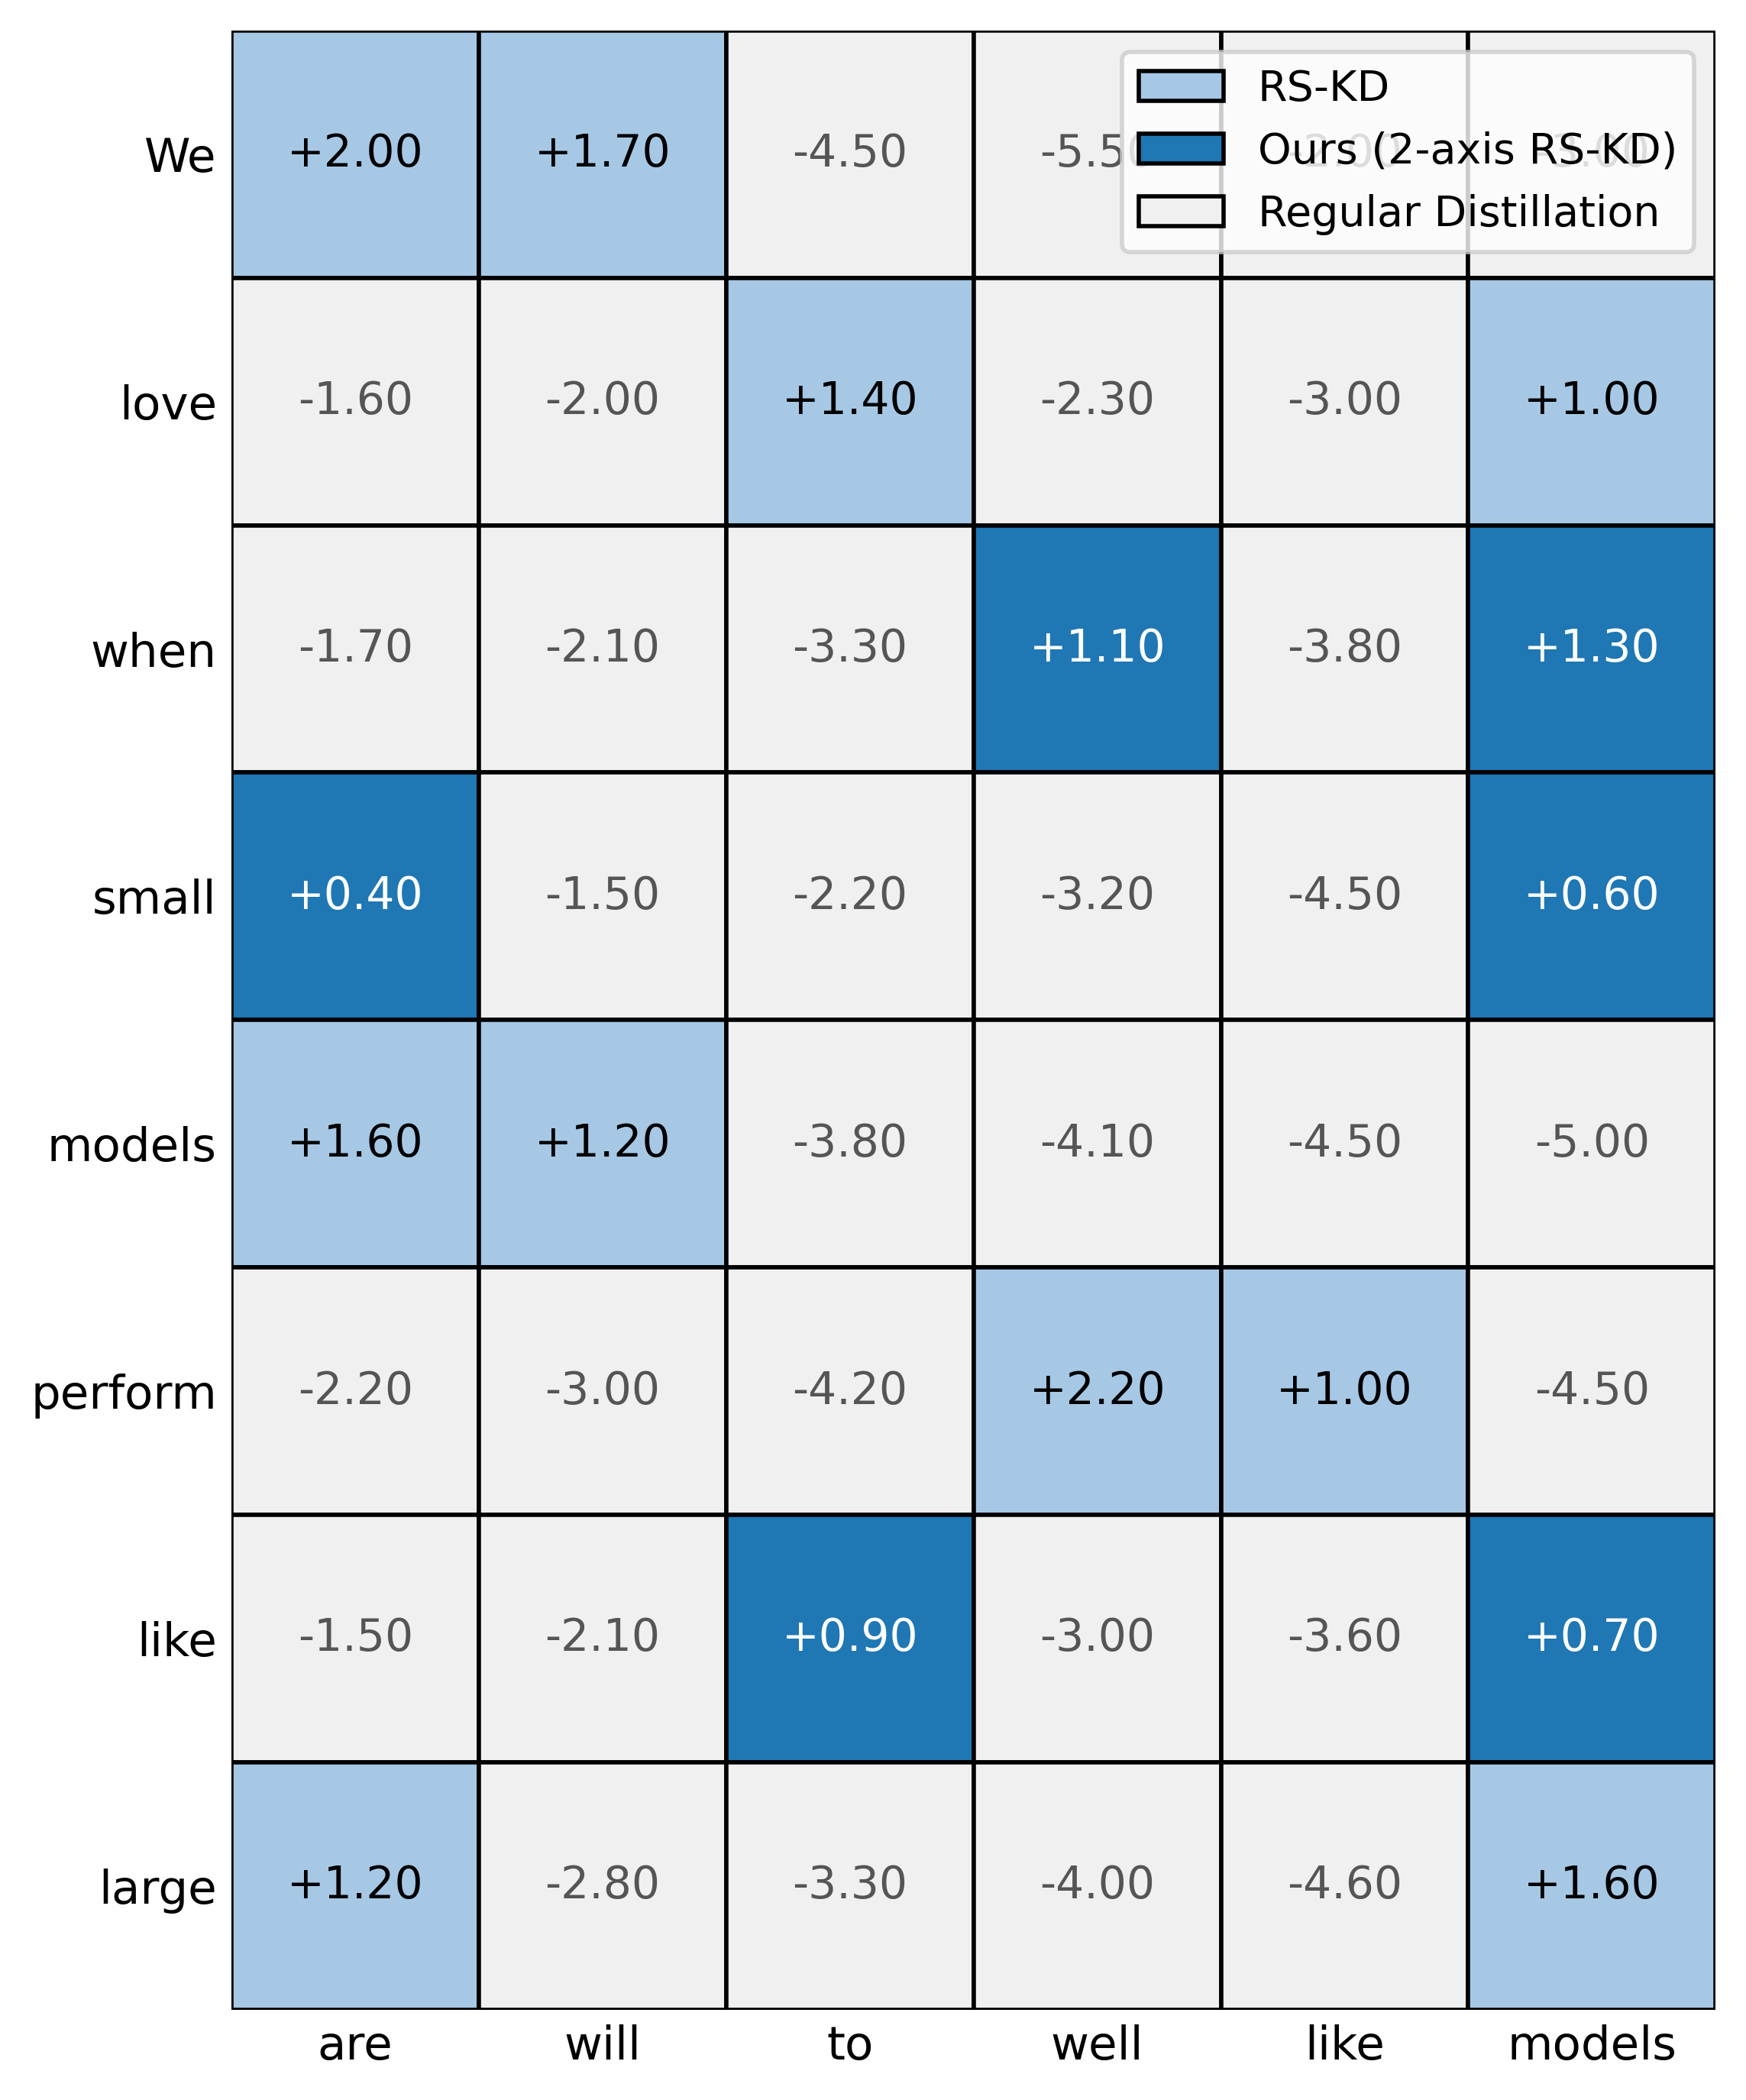
\includegraphics[width=\linewidth]{rskd_grid_two_axis_blue.png}
	\resizebox{\columnwidth}{!}{%% Creator: Matplotlib, PGF backend
%%
%% To include the figure in your LaTeX document, write
%%   \input{<filename>.pgf}
%%
%% Make sure the required packages are loaded in your preamble
%%   \usepackage{pgf}
%%
%% Also ensure that all the required font packages are loaded; for instance,
%% the lmodern package is sometimes necessary when using math font.
%%   \usepackage{lmodern}
%%
%% Figures using additional raster images can only be included by \input if
%% they are in the same directory as the main LaTeX file. For loading figures
%% from other directories you can use the `import` package
%%   \usepackage{import}
%%
%% and then include the figures with
%%   \import{<path to file>}{<filename>.pgf}
%%
%% Matplotlib used the following preamble
%%   \def\mathdefault#1{#1}
%%   \everymath=\expandafter{\the\everymath\displaystyle}
%%   \IfFileExists{scrextend.sty}{
%%     \usepackage[fontsize=10.000000pt]{scrextend}
%%   }{
%%     \renewcommand{\normalsize}{\fontsize{10.000000}{12.000000}\selectfont}
%%     \normalsize
%%   }
%%   
%%   \makeatletter\@ifpackageloaded{underscore}{}{\usepackage[strings]{underscore}}\makeatother
%%
\begingroup%
\makeatletter%
\begin{pgfpicture}%
\pgfpathrectangle{\pgfpointorigin}{\pgfqpoint{5.505730in}{6.670422in}}%
\pgfusepath{use as bounding box, clip}%
\begin{pgfscope}%
\pgfsetbuttcap%
\pgfsetmiterjoin%
\definecolor{currentfill}{rgb}{1.000000,1.000000,1.000000}%
\pgfsetfillcolor{currentfill}%
\pgfsetlinewidth{0.000000pt}%
\definecolor{currentstroke}{rgb}{1.000000,1.000000,1.000000}%
\pgfsetstrokecolor{currentstroke}%
\pgfsetdash{}{0pt}%
\pgfpathmoveto{\pgfqpoint{0.000000in}{0.000000in}}%
\pgfpathlineto{\pgfqpoint{5.505730in}{0.000000in}}%
\pgfpathlineto{\pgfqpoint{5.505730in}{6.670422in}}%
\pgfpathlineto{\pgfqpoint{0.000000in}{6.670422in}}%
\pgfpathlineto{\pgfqpoint{0.000000in}{0.000000in}}%
\pgfpathclose%
\pgfusepath{fill}%
\end{pgfscope}%
\begin{pgfscope}%
\pgfsetbuttcap%
\pgfsetmiterjoin%
\definecolor{currentfill}{rgb}{1.000000,1.000000,1.000000}%
\pgfsetfillcolor{currentfill}%
\pgfsetlinewidth{0.000000pt}%
\definecolor{currentstroke}{rgb}{0.000000,0.000000,0.000000}%
\pgfsetstrokecolor{currentstroke}%
\pgfsetstrokeopacity{0.000000}%
\pgfsetdash{}{0pt}%
\pgfpathmoveto{\pgfqpoint{0.846963in}{0.458732in}}%
\pgfpathlineto{\pgfqpoint{5.505730in}{0.458732in}}%
\pgfpathlineto{\pgfqpoint{5.505730in}{6.670422in}}%
\pgfpathlineto{\pgfqpoint{0.846963in}{6.670422in}}%
\pgfpathlineto{\pgfqpoint{0.846963in}{0.458732in}}%
\pgfpathclose%
\pgfusepath{fill}%
\end{pgfscope}%
\begin{pgfscope}%
\pgfpathrectangle{\pgfqpoint{0.846963in}{0.458732in}}{\pgfqpoint{4.658768in}{6.211690in}}%
\pgfusepath{clip}%
\pgfsetbuttcap%
\pgfsetmiterjoin%
\definecolor{currentfill}{rgb}{0.650980,0.784314,0.898039}%
\pgfsetfillcolor{currentfill}%
\pgfsetlinewidth{1.003750pt}%
\definecolor{currentstroke}{rgb}{0.000000,0.000000,0.000000}%
\pgfsetstrokecolor{currentstroke}%
\pgfsetdash{}{0pt}%
\pgfpathmoveto{\pgfqpoint{0.846963in}{6.670422in}}%
\pgfpathlineto{\pgfqpoint{1.623424in}{6.670422in}}%
\pgfpathlineto{\pgfqpoint{1.623424in}{5.893961in}}%
\pgfpathlineto{\pgfqpoint{0.846963in}{5.893961in}}%
\pgfpathlineto{\pgfqpoint{0.846963in}{6.670422in}}%
\pgfpathclose%
\pgfusepath{stroke,fill}%
\end{pgfscope}%
\begin{pgfscope}%
\pgfpathrectangle{\pgfqpoint{0.846963in}{0.458732in}}{\pgfqpoint{4.658768in}{6.211690in}}%
\pgfusepath{clip}%
\pgfsetbuttcap%
\pgfsetmiterjoin%
\definecolor{currentfill}{rgb}{0.650980,0.784314,0.898039}%
\pgfsetfillcolor{currentfill}%
\pgfsetlinewidth{1.003750pt}%
\definecolor{currentstroke}{rgb}{0.000000,0.000000,0.000000}%
\pgfsetstrokecolor{currentstroke}%
\pgfsetdash{}{0pt}%
\pgfpathmoveto{\pgfqpoint{1.623424in}{6.670422in}}%
\pgfpathlineto{\pgfqpoint{2.399885in}{6.670422in}}%
\pgfpathlineto{\pgfqpoint{2.399885in}{5.893961in}}%
\pgfpathlineto{\pgfqpoint{1.623424in}{5.893961in}}%
\pgfpathlineto{\pgfqpoint{1.623424in}{6.670422in}}%
\pgfpathclose%
\pgfusepath{stroke,fill}%
\end{pgfscope}%
\begin{pgfscope}%
\pgfpathrectangle{\pgfqpoint{0.846963in}{0.458732in}}{\pgfqpoint{4.658768in}{6.211690in}}%
\pgfusepath{clip}%
\pgfsetbuttcap%
\pgfsetmiterjoin%
\definecolor{currentfill}{rgb}{0.941176,0.941176,0.941176}%
\pgfsetfillcolor{currentfill}%
\pgfsetlinewidth{1.003750pt}%
\definecolor{currentstroke}{rgb}{0.000000,0.000000,0.000000}%
\pgfsetstrokecolor{currentstroke}%
\pgfsetdash{}{0pt}%
\pgfpathmoveto{\pgfqpoint{2.399885in}{6.670422in}}%
\pgfpathlineto{\pgfqpoint{3.176347in}{6.670422in}}%
\pgfpathlineto{\pgfqpoint{3.176347in}{5.893961in}}%
\pgfpathlineto{\pgfqpoint{2.399885in}{5.893961in}}%
\pgfpathlineto{\pgfqpoint{2.399885in}{6.670422in}}%
\pgfpathclose%
\pgfusepath{stroke,fill}%
\end{pgfscope}%
\begin{pgfscope}%
\pgfpathrectangle{\pgfqpoint{0.846963in}{0.458732in}}{\pgfqpoint{4.658768in}{6.211690in}}%
\pgfusepath{clip}%
\pgfsetbuttcap%
\pgfsetmiterjoin%
\definecolor{currentfill}{rgb}{0.941176,0.941176,0.941176}%
\pgfsetfillcolor{currentfill}%
\pgfsetlinewidth{1.003750pt}%
\definecolor{currentstroke}{rgb}{0.000000,0.000000,0.000000}%
\pgfsetstrokecolor{currentstroke}%
\pgfsetdash{}{0pt}%
\pgfpathmoveto{\pgfqpoint{3.176347in}{6.670422in}}%
\pgfpathlineto{\pgfqpoint{3.952808in}{6.670422in}}%
\pgfpathlineto{\pgfqpoint{3.952808in}{5.893961in}}%
\pgfpathlineto{\pgfqpoint{3.176347in}{5.893961in}}%
\pgfpathlineto{\pgfqpoint{3.176347in}{6.670422in}}%
\pgfpathclose%
\pgfusepath{stroke,fill}%
\end{pgfscope}%
\begin{pgfscope}%
\pgfpathrectangle{\pgfqpoint{0.846963in}{0.458732in}}{\pgfqpoint{4.658768in}{6.211690in}}%
\pgfusepath{clip}%
\pgfsetbuttcap%
\pgfsetmiterjoin%
\definecolor{currentfill}{rgb}{0.941176,0.941176,0.941176}%
\pgfsetfillcolor{currentfill}%
\pgfsetlinewidth{1.003750pt}%
\definecolor{currentstroke}{rgb}{0.000000,0.000000,0.000000}%
\pgfsetstrokecolor{currentstroke}%
\pgfsetdash{}{0pt}%
\pgfpathmoveto{\pgfqpoint{3.952808in}{6.670422in}}%
\pgfpathlineto{\pgfqpoint{4.729269in}{6.670422in}}%
\pgfpathlineto{\pgfqpoint{4.729269in}{5.893961in}}%
\pgfpathlineto{\pgfqpoint{3.952808in}{5.893961in}}%
\pgfpathlineto{\pgfqpoint{3.952808in}{6.670422in}}%
\pgfpathclose%
\pgfusepath{stroke,fill}%
\end{pgfscope}%
\begin{pgfscope}%
\pgfpathrectangle{\pgfqpoint{0.846963in}{0.458732in}}{\pgfqpoint{4.658768in}{6.211690in}}%
\pgfusepath{clip}%
\pgfsetbuttcap%
\pgfsetmiterjoin%
\definecolor{currentfill}{rgb}{0.941176,0.941176,0.941176}%
\pgfsetfillcolor{currentfill}%
\pgfsetlinewidth{1.003750pt}%
\definecolor{currentstroke}{rgb}{0.000000,0.000000,0.000000}%
\pgfsetstrokecolor{currentstroke}%
\pgfsetdash{}{0pt}%
\pgfpathmoveto{\pgfqpoint{4.729269in}{6.670422in}}%
\pgfpathlineto{\pgfqpoint{5.505730in}{6.670422in}}%
\pgfpathlineto{\pgfqpoint{5.505730in}{5.893961in}}%
\pgfpathlineto{\pgfqpoint{4.729269in}{5.893961in}}%
\pgfpathlineto{\pgfqpoint{4.729269in}{6.670422in}}%
\pgfpathclose%
\pgfusepath{stroke,fill}%
\end{pgfscope}%
\begin{pgfscope}%
\pgfpathrectangle{\pgfqpoint{0.846963in}{0.458732in}}{\pgfqpoint{4.658768in}{6.211690in}}%
\pgfusepath{clip}%
\pgfsetbuttcap%
\pgfsetmiterjoin%
\definecolor{currentfill}{rgb}{0.941176,0.941176,0.941176}%
\pgfsetfillcolor{currentfill}%
\pgfsetlinewidth{1.003750pt}%
\definecolor{currentstroke}{rgb}{0.000000,0.000000,0.000000}%
\pgfsetstrokecolor{currentstroke}%
\pgfsetdash{}{0pt}%
\pgfpathmoveto{\pgfqpoint{0.846963in}{5.893961in}}%
\pgfpathlineto{\pgfqpoint{1.623424in}{5.893961in}}%
\pgfpathlineto{\pgfqpoint{1.623424in}{5.117500in}}%
\pgfpathlineto{\pgfqpoint{0.846963in}{5.117500in}}%
\pgfpathlineto{\pgfqpoint{0.846963in}{5.893961in}}%
\pgfpathclose%
\pgfusepath{stroke,fill}%
\end{pgfscope}%
\begin{pgfscope}%
\pgfpathrectangle{\pgfqpoint{0.846963in}{0.458732in}}{\pgfqpoint{4.658768in}{6.211690in}}%
\pgfusepath{clip}%
\pgfsetbuttcap%
\pgfsetmiterjoin%
\definecolor{currentfill}{rgb}{0.941176,0.941176,0.941176}%
\pgfsetfillcolor{currentfill}%
\pgfsetlinewidth{1.003750pt}%
\definecolor{currentstroke}{rgb}{0.000000,0.000000,0.000000}%
\pgfsetstrokecolor{currentstroke}%
\pgfsetdash{}{0pt}%
\pgfpathmoveto{\pgfqpoint{1.623424in}{5.893961in}}%
\pgfpathlineto{\pgfqpoint{2.399885in}{5.893961in}}%
\pgfpathlineto{\pgfqpoint{2.399885in}{5.117500in}}%
\pgfpathlineto{\pgfqpoint{1.623424in}{5.117500in}}%
\pgfpathlineto{\pgfqpoint{1.623424in}{5.893961in}}%
\pgfpathclose%
\pgfusepath{stroke,fill}%
\end{pgfscope}%
\begin{pgfscope}%
\pgfpathrectangle{\pgfqpoint{0.846963in}{0.458732in}}{\pgfqpoint{4.658768in}{6.211690in}}%
\pgfusepath{clip}%
\pgfsetbuttcap%
\pgfsetmiterjoin%
\definecolor{currentfill}{rgb}{0.650980,0.784314,0.898039}%
\pgfsetfillcolor{currentfill}%
\pgfsetlinewidth{1.003750pt}%
\definecolor{currentstroke}{rgb}{0.000000,0.000000,0.000000}%
\pgfsetstrokecolor{currentstroke}%
\pgfsetdash{}{0pt}%
\pgfpathmoveto{\pgfqpoint{2.399885in}{5.893961in}}%
\pgfpathlineto{\pgfqpoint{3.176347in}{5.893961in}}%
\pgfpathlineto{\pgfqpoint{3.176347in}{5.117500in}}%
\pgfpathlineto{\pgfqpoint{2.399885in}{5.117500in}}%
\pgfpathlineto{\pgfqpoint{2.399885in}{5.893961in}}%
\pgfpathclose%
\pgfusepath{stroke,fill}%
\end{pgfscope}%
\begin{pgfscope}%
\pgfpathrectangle{\pgfqpoint{0.846963in}{0.458732in}}{\pgfqpoint{4.658768in}{6.211690in}}%
\pgfusepath{clip}%
\pgfsetbuttcap%
\pgfsetmiterjoin%
\definecolor{currentfill}{rgb}{0.941176,0.941176,0.941176}%
\pgfsetfillcolor{currentfill}%
\pgfsetlinewidth{1.003750pt}%
\definecolor{currentstroke}{rgb}{0.000000,0.000000,0.000000}%
\pgfsetstrokecolor{currentstroke}%
\pgfsetdash{}{0pt}%
\pgfpathmoveto{\pgfqpoint{3.176347in}{5.893961in}}%
\pgfpathlineto{\pgfqpoint{3.952808in}{5.893961in}}%
\pgfpathlineto{\pgfqpoint{3.952808in}{5.117500in}}%
\pgfpathlineto{\pgfqpoint{3.176347in}{5.117500in}}%
\pgfpathlineto{\pgfqpoint{3.176347in}{5.893961in}}%
\pgfpathclose%
\pgfusepath{stroke,fill}%
\end{pgfscope}%
\begin{pgfscope}%
\pgfpathrectangle{\pgfqpoint{0.846963in}{0.458732in}}{\pgfqpoint{4.658768in}{6.211690in}}%
\pgfusepath{clip}%
\pgfsetbuttcap%
\pgfsetmiterjoin%
\definecolor{currentfill}{rgb}{0.941176,0.941176,0.941176}%
\pgfsetfillcolor{currentfill}%
\pgfsetlinewidth{1.003750pt}%
\definecolor{currentstroke}{rgb}{0.000000,0.000000,0.000000}%
\pgfsetstrokecolor{currentstroke}%
\pgfsetdash{}{0pt}%
\pgfpathmoveto{\pgfqpoint{3.952808in}{5.893961in}}%
\pgfpathlineto{\pgfqpoint{4.729269in}{5.893961in}}%
\pgfpathlineto{\pgfqpoint{4.729269in}{5.117500in}}%
\pgfpathlineto{\pgfqpoint{3.952808in}{5.117500in}}%
\pgfpathlineto{\pgfqpoint{3.952808in}{5.893961in}}%
\pgfpathclose%
\pgfusepath{stroke,fill}%
\end{pgfscope}%
\begin{pgfscope}%
\pgfpathrectangle{\pgfqpoint{0.846963in}{0.458732in}}{\pgfqpoint{4.658768in}{6.211690in}}%
\pgfusepath{clip}%
\pgfsetbuttcap%
\pgfsetmiterjoin%
\definecolor{currentfill}{rgb}{0.650980,0.784314,0.898039}%
\pgfsetfillcolor{currentfill}%
\pgfsetlinewidth{1.003750pt}%
\definecolor{currentstroke}{rgb}{0.000000,0.000000,0.000000}%
\pgfsetstrokecolor{currentstroke}%
\pgfsetdash{}{0pt}%
\pgfpathmoveto{\pgfqpoint{4.729269in}{5.893961in}}%
\pgfpathlineto{\pgfqpoint{5.505730in}{5.893961in}}%
\pgfpathlineto{\pgfqpoint{5.505730in}{5.117500in}}%
\pgfpathlineto{\pgfqpoint{4.729269in}{5.117500in}}%
\pgfpathlineto{\pgfqpoint{4.729269in}{5.893961in}}%
\pgfpathclose%
\pgfusepath{stroke,fill}%
\end{pgfscope}%
\begin{pgfscope}%
\pgfpathrectangle{\pgfqpoint{0.846963in}{0.458732in}}{\pgfqpoint{4.658768in}{6.211690in}}%
\pgfusepath{clip}%
\pgfsetbuttcap%
\pgfsetmiterjoin%
\definecolor{currentfill}{rgb}{0.941176,0.941176,0.941176}%
\pgfsetfillcolor{currentfill}%
\pgfsetlinewidth{1.003750pt}%
\definecolor{currentstroke}{rgb}{0.000000,0.000000,0.000000}%
\pgfsetstrokecolor{currentstroke}%
\pgfsetdash{}{0pt}%
\pgfpathmoveto{\pgfqpoint{0.846963in}{5.117500in}}%
\pgfpathlineto{\pgfqpoint{1.623424in}{5.117500in}}%
\pgfpathlineto{\pgfqpoint{1.623424in}{4.341039in}}%
\pgfpathlineto{\pgfqpoint{0.846963in}{4.341039in}}%
\pgfpathlineto{\pgfqpoint{0.846963in}{5.117500in}}%
\pgfpathclose%
\pgfusepath{stroke,fill}%
\end{pgfscope}%
\begin{pgfscope}%
\pgfpathrectangle{\pgfqpoint{0.846963in}{0.458732in}}{\pgfqpoint{4.658768in}{6.211690in}}%
\pgfusepath{clip}%
\pgfsetbuttcap%
\pgfsetmiterjoin%
\definecolor{currentfill}{rgb}{0.941176,0.941176,0.941176}%
\pgfsetfillcolor{currentfill}%
\pgfsetlinewidth{1.003750pt}%
\definecolor{currentstroke}{rgb}{0.000000,0.000000,0.000000}%
\pgfsetstrokecolor{currentstroke}%
\pgfsetdash{}{0pt}%
\pgfpathmoveto{\pgfqpoint{1.623424in}{5.117500in}}%
\pgfpathlineto{\pgfqpoint{2.399885in}{5.117500in}}%
\pgfpathlineto{\pgfqpoint{2.399885in}{4.341039in}}%
\pgfpathlineto{\pgfqpoint{1.623424in}{4.341039in}}%
\pgfpathlineto{\pgfqpoint{1.623424in}{5.117500in}}%
\pgfpathclose%
\pgfusepath{stroke,fill}%
\end{pgfscope}%
\begin{pgfscope}%
\pgfpathrectangle{\pgfqpoint{0.846963in}{0.458732in}}{\pgfqpoint{4.658768in}{6.211690in}}%
\pgfusepath{clip}%
\pgfsetbuttcap%
\pgfsetmiterjoin%
\definecolor{currentfill}{rgb}{0.941176,0.941176,0.941176}%
\pgfsetfillcolor{currentfill}%
\pgfsetlinewidth{1.003750pt}%
\definecolor{currentstroke}{rgb}{0.000000,0.000000,0.000000}%
\pgfsetstrokecolor{currentstroke}%
\pgfsetdash{}{0pt}%
\pgfpathmoveto{\pgfqpoint{2.399885in}{5.117500in}}%
\pgfpathlineto{\pgfqpoint{3.176347in}{5.117500in}}%
\pgfpathlineto{\pgfqpoint{3.176347in}{4.341039in}}%
\pgfpathlineto{\pgfqpoint{2.399885in}{4.341039in}}%
\pgfpathlineto{\pgfqpoint{2.399885in}{5.117500in}}%
\pgfpathclose%
\pgfusepath{stroke,fill}%
\end{pgfscope}%
\begin{pgfscope}%
\pgfpathrectangle{\pgfqpoint{0.846963in}{0.458732in}}{\pgfqpoint{4.658768in}{6.211690in}}%
\pgfusepath{clip}%
\pgfsetbuttcap%
\pgfsetmiterjoin%
\definecolor{currentfill}{rgb}{0.121569,0.466667,0.705882}%
\pgfsetfillcolor{currentfill}%
\pgfsetlinewidth{1.003750pt}%
\definecolor{currentstroke}{rgb}{0.000000,0.000000,0.000000}%
\pgfsetstrokecolor{currentstroke}%
\pgfsetdash{}{0pt}%
\pgfpathmoveto{\pgfqpoint{3.176347in}{5.117500in}}%
\pgfpathlineto{\pgfqpoint{3.952808in}{5.117500in}}%
\pgfpathlineto{\pgfqpoint{3.952808in}{4.341039in}}%
\pgfpathlineto{\pgfqpoint{3.176347in}{4.341039in}}%
\pgfpathlineto{\pgfqpoint{3.176347in}{5.117500in}}%
\pgfpathclose%
\pgfusepath{stroke,fill}%
\end{pgfscope}%
\begin{pgfscope}%
\pgfpathrectangle{\pgfqpoint{0.846963in}{0.458732in}}{\pgfqpoint{4.658768in}{6.211690in}}%
\pgfusepath{clip}%
\pgfsetbuttcap%
\pgfsetmiterjoin%
\definecolor{currentfill}{rgb}{0.941176,0.941176,0.941176}%
\pgfsetfillcolor{currentfill}%
\pgfsetlinewidth{1.003750pt}%
\definecolor{currentstroke}{rgb}{0.000000,0.000000,0.000000}%
\pgfsetstrokecolor{currentstroke}%
\pgfsetdash{}{0pt}%
\pgfpathmoveto{\pgfqpoint{3.952808in}{5.117500in}}%
\pgfpathlineto{\pgfqpoint{4.729269in}{5.117500in}}%
\pgfpathlineto{\pgfqpoint{4.729269in}{4.341039in}}%
\pgfpathlineto{\pgfqpoint{3.952808in}{4.341039in}}%
\pgfpathlineto{\pgfqpoint{3.952808in}{5.117500in}}%
\pgfpathclose%
\pgfusepath{stroke,fill}%
\end{pgfscope}%
\begin{pgfscope}%
\pgfpathrectangle{\pgfqpoint{0.846963in}{0.458732in}}{\pgfqpoint{4.658768in}{6.211690in}}%
\pgfusepath{clip}%
\pgfsetbuttcap%
\pgfsetmiterjoin%
\definecolor{currentfill}{rgb}{0.121569,0.466667,0.705882}%
\pgfsetfillcolor{currentfill}%
\pgfsetlinewidth{1.003750pt}%
\definecolor{currentstroke}{rgb}{0.000000,0.000000,0.000000}%
\pgfsetstrokecolor{currentstroke}%
\pgfsetdash{}{0pt}%
\pgfpathmoveto{\pgfqpoint{4.729269in}{5.117500in}}%
\pgfpathlineto{\pgfqpoint{5.505730in}{5.117500in}}%
\pgfpathlineto{\pgfqpoint{5.505730in}{4.341039in}}%
\pgfpathlineto{\pgfqpoint{4.729269in}{4.341039in}}%
\pgfpathlineto{\pgfqpoint{4.729269in}{5.117500in}}%
\pgfpathclose%
\pgfusepath{stroke,fill}%
\end{pgfscope}%
\begin{pgfscope}%
\pgfpathrectangle{\pgfqpoint{0.846963in}{0.458732in}}{\pgfqpoint{4.658768in}{6.211690in}}%
\pgfusepath{clip}%
\pgfsetbuttcap%
\pgfsetmiterjoin%
\definecolor{currentfill}{rgb}{0.121569,0.466667,0.705882}%
\pgfsetfillcolor{currentfill}%
\pgfsetlinewidth{1.003750pt}%
\definecolor{currentstroke}{rgb}{0.000000,0.000000,0.000000}%
\pgfsetstrokecolor{currentstroke}%
\pgfsetdash{}{0pt}%
\pgfpathmoveto{\pgfqpoint{0.846963in}{4.341039in}}%
\pgfpathlineto{\pgfqpoint{1.623424in}{4.341039in}}%
\pgfpathlineto{\pgfqpoint{1.623424in}{3.564577in}}%
\pgfpathlineto{\pgfqpoint{0.846963in}{3.564577in}}%
\pgfpathlineto{\pgfqpoint{0.846963in}{4.341039in}}%
\pgfpathclose%
\pgfusepath{stroke,fill}%
\end{pgfscope}%
\begin{pgfscope}%
\pgfpathrectangle{\pgfqpoint{0.846963in}{0.458732in}}{\pgfqpoint{4.658768in}{6.211690in}}%
\pgfusepath{clip}%
\pgfsetbuttcap%
\pgfsetmiterjoin%
\definecolor{currentfill}{rgb}{0.941176,0.941176,0.941176}%
\pgfsetfillcolor{currentfill}%
\pgfsetlinewidth{1.003750pt}%
\definecolor{currentstroke}{rgb}{0.000000,0.000000,0.000000}%
\pgfsetstrokecolor{currentstroke}%
\pgfsetdash{}{0pt}%
\pgfpathmoveto{\pgfqpoint{1.623424in}{4.341039in}}%
\pgfpathlineto{\pgfqpoint{2.399885in}{4.341039in}}%
\pgfpathlineto{\pgfqpoint{2.399885in}{3.564577in}}%
\pgfpathlineto{\pgfqpoint{1.623424in}{3.564577in}}%
\pgfpathlineto{\pgfqpoint{1.623424in}{4.341039in}}%
\pgfpathclose%
\pgfusepath{stroke,fill}%
\end{pgfscope}%
\begin{pgfscope}%
\pgfpathrectangle{\pgfqpoint{0.846963in}{0.458732in}}{\pgfqpoint{4.658768in}{6.211690in}}%
\pgfusepath{clip}%
\pgfsetbuttcap%
\pgfsetmiterjoin%
\definecolor{currentfill}{rgb}{0.941176,0.941176,0.941176}%
\pgfsetfillcolor{currentfill}%
\pgfsetlinewidth{1.003750pt}%
\definecolor{currentstroke}{rgb}{0.000000,0.000000,0.000000}%
\pgfsetstrokecolor{currentstroke}%
\pgfsetdash{}{0pt}%
\pgfpathmoveto{\pgfqpoint{2.399885in}{4.341039in}}%
\pgfpathlineto{\pgfqpoint{3.176347in}{4.341039in}}%
\pgfpathlineto{\pgfqpoint{3.176347in}{3.564577in}}%
\pgfpathlineto{\pgfqpoint{2.399885in}{3.564577in}}%
\pgfpathlineto{\pgfqpoint{2.399885in}{4.341039in}}%
\pgfpathclose%
\pgfusepath{stroke,fill}%
\end{pgfscope}%
\begin{pgfscope}%
\pgfpathrectangle{\pgfqpoint{0.846963in}{0.458732in}}{\pgfqpoint{4.658768in}{6.211690in}}%
\pgfusepath{clip}%
\pgfsetbuttcap%
\pgfsetmiterjoin%
\definecolor{currentfill}{rgb}{0.941176,0.941176,0.941176}%
\pgfsetfillcolor{currentfill}%
\pgfsetlinewidth{1.003750pt}%
\definecolor{currentstroke}{rgb}{0.000000,0.000000,0.000000}%
\pgfsetstrokecolor{currentstroke}%
\pgfsetdash{}{0pt}%
\pgfpathmoveto{\pgfqpoint{3.176347in}{4.341039in}}%
\pgfpathlineto{\pgfqpoint{3.952808in}{4.341039in}}%
\pgfpathlineto{\pgfqpoint{3.952808in}{3.564577in}}%
\pgfpathlineto{\pgfqpoint{3.176347in}{3.564577in}}%
\pgfpathlineto{\pgfqpoint{3.176347in}{4.341039in}}%
\pgfpathclose%
\pgfusepath{stroke,fill}%
\end{pgfscope}%
\begin{pgfscope}%
\pgfpathrectangle{\pgfqpoint{0.846963in}{0.458732in}}{\pgfqpoint{4.658768in}{6.211690in}}%
\pgfusepath{clip}%
\pgfsetbuttcap%
\pgfsetmiterjoin%
\definecolor{currentfill}{rgb}{0.941176,0.941176,0.941176}%
\pgfsetfillcolor{currentfill}%
\pgfsetlinewidth{1.003750pt}%
\definecolor{currentstroke}{rgb}{0.000000,0.000000,0.000000}%
\pgfsetstrokecolor{currentstroke}%
\pgfsetdash{}{0pt}%
\pgfpathmoveto{\pgfqpoint{3.952808in}{4.341039in}}%
\pgfpathlineto{\pgfqpoint{4.729269in}{4.341039in}}%
\pgfpathlineto{\pgfqpoint{4.729269in}{3.564577in}}%
\pgfpathlineto{\pgfqpoint{3.952808in}{3.564577in}}%
\pgfpathlineto{\pgfqpoint{3.952808in}{4.341039in}}%
\pgfpathclose%
\pgfusepath{stroke,fill}%
\end{pgfscope}%
\begin{pgfscope}%
\pgfpathrectangle{\pgfqpoint{0.846963in}{0.458732in}}{\pgfqpoint{4.658768in}{6.211690in}}%
\pgfusepath{clip}%
\pgfsetbuttcap%
\pgfsetmiterjoin%
\definecolor{currentfill}{rgb}{0.121569,0.466667,0.705882}%
\pgfsetfillcolor{currentfill}%
\pgfsetlinewidth{1.003750pt}%
\definecolor{currentstroke}{rgb}{0.000000,0.000000,0.000000}%
\pgfsetstrokecolor{currentstroke}%
\pgfsetdash{}{0pt}%
\pgfpathmoveto{\pgfqpoint{4.729269in}{4.341039in}}%
\pgfpathlineto{\pgfqpoint{5.505730in}{4.341039in}}%
\pgfpathlineto{\pgfqpoint{5.505730in}{3.564577in}}%
\pgfpathlineto{\pgfqpoint{4.729269in}{3.564577in}}%
\pgfpathlineto{\pgfqpoint{4.729269in}{4.341039in}}%
\pgfpathclose%
\pgfusepath{stroke,fill}%
\end{pgfscope}%
\begin{pgfscope}%
\pgfpathrectangle{\pgfqpoint{0.846963in}{0.458732in}}{\pgfqpoint{4.658768in}{6.211690in}}%
\pgfusepath{clip}%
\pgfsetbuttcap%
\pgfsetmiterjoin%
\definecolor{currentfill}{rgb}{0.650980,0.784314,0.898039}%
\pgfsetfillcolor{currentfill}%
\pgfsetlinewidth{1.003750pt}%
\definecolor{currentstroke}{rgb}{0.000000,0.000000,0.000000}%
\pgfsetstrokecolor{currentstroke}%
\pgfsetdash{}{0pt}%
\pgfpathmoveto{\pgfqpoint{0.846963in}{3.564577in}}%
\pgfpathlineto{\pgfqpoint{1.623424in}{3.564577in}}%
\pgfpathlineto{\pgfqpoint{1.623424in}{2.788116in}}%
\pgfpathlineto{\pgfqpoint{0.846963in}{2.788116in}}%
\pgfpathlineto{\pgfqpoint{0.846963in}{3.564577in}}%
\pgfpathclose%
\pgfusepath{stroke,fill}%
\end{pgfscope}%
\begin{pgfscope}%
\pgfpathrectangle{\pgfqpoint{0.846963in}{0.458732in}}{\pgfqpoint{4.658768in}{6.211690in}}%
\pgfusepath{clip}%
\pgfsetbuttcap%
\pgfsetmiterjoin%
\definecolor{currentfill}{rgb}{0.650980,0.784314,0.898039}%
\pgfsetfillcolor{currentfill}%
\pgfsetlinewidth{1.003750pt}%
\definecolor{currentstroke}{rgb}{0.000000,0.000000,0.000000}%
\pgfsetstrokecolor{currentstroke}%
\pgfsetdash{}{0pt}%
\pgfpathmoveto{\pgfqpoint{1.623424in}{3.564577in}}%
\pgfpathlineto{\pgfqpoint{2.399885in}{3.564577in}}%
\pgfpathlineto{\pgfqpoint{2.399885in}{2.788116in}}%
\pgfpathlineto{\pgfqpoint{1.623424in}{2.788116in}}%
\pgfpathlineto{\pgfqpoint{1.623424in}{3.564577in}}%
\pgfpathclose%
\pgfusepath{stroke,fill}%
\end{pgfscope}%
\begin{pgfscope}%
\pgfpathrectangle{\pgfqpoint{0.846963in}{0.458732in}}{\pgfqpoint{4.658768in}{6.211690in}}%
\pgfusepath{clip}%
\pgfsetbuttcap%
\pgfsetmiterjoin%
\definecolor{currentfill}{rgb}{0.941176,0.941176,0.941176}%
\pgfsetfillcolor{currentfill}%
\pgfsetlinewidth{1.003750pt}%
\definecolor{currentstroke}{rgb}{0.000000,0.000000,0.000000}%
\pgfsetstrokecolor{currentstroke}%
\pgfsetdash{}{0pt}%
\pgfpathmoveto{\pgfqpoint{2.399885in}{3.564577in}}%
\pgfpathlineto{\pgfqpoint{3.176347in}{3.564577in}}%
\pgfpathlineto{\pgfqpoint{3.176347in}{2.788116in}}%
\pgfpathlineto{\pgfqpoint{2.399885in}{2.788116in}}%
\pgfpathlineto{\pgfqpoint{2.399885in}{3.564577in}}%
\pgfpathclose%
\pgfusepath{stroke,fill}%
\end{pgfscope}%
\begin{pgfscope}%
\pgfpathrectangle{\pgfqpoint{0.846963in}{0.458732in}}{\pgfqpoint{4.658768in}{6.211690in}}%
\pgfusepath{clip}%
\pgfsetbuttcap%
\pgfsetmiterjoin%
\definecolor{currentfill}{rgb}{0.941176,0.941176,0.941176}%
\pgfsetfillcolor{currentfill}%
\pgfsetlinewidth{1.003750pt}%
\definecolor{currentstroke}{rgb}{0.000000,0.000000,0.000000}%
\pgfsetstrokecolor{currentstroke}%
\pgfsetdash{}{0pt}%
\pgfpathmoveto{\pgfqpoint{3.176347in}{3.564577in}}%
\pgfpathlineto{\pgfqpoint{3.952808in}{3.564577in}}%
\pgfpathlineto{\pgfqpoint{3.952808in}{2.788116in}}%
\pgfpathlineto{\pgfqpoint{3.176347in}{2.788116in}}%
\pgfpathlineto{\pgfqpoint{3.176347in}{3.564577in}}%
\pgfpathclose%
\pgfusepath{stroke,fill}%
\end{pgfscope}%
\begin{pgfscope}%
\pgfpathrectangle{\pgfqpoint{0.846963in}{0.458732in}}{\pgfqpoint{4.658768in}{6.211690in}}%
\pgfusepath{clip}%
\pgfsetbuttcap%
\pgfsetmiterjoin%
\definecolor{currentfill}{rgb}{0.941176,0.941176,0.941176}%
\pgfsetfillcolor{currentfill}%
\pgfsetlinewidth{1.003750pt}%
\definecolor{currentstroke}{rgb}{0.000000,0.000000,0.000000}%
\pgfsetstrokecolor{currentstroke}%
\pgfsetdash{}{0pt}%
\pgfpathmoveto{\pgfqpoint{3.952808in}{3.564577in}}%
\pgfpathlineto{\pgfqpoint{4.729269in}{3.564577in}}%
\pgfpathlineto{\pgfqpoint{4.729269in}{2.788116in}}%
\pgfpathlineto{\pgfqpoint{3.952808in}{2.788116in}}%
\pgfpathlineto{\pgfqpoint{3.952808in}{3.564577in}}%
\pgfpathclose%
\pgfusepath{stroke,fill}%
\end{pgfscope}%
\begin{pgfscope}%
\pgfpathrectangle{\pgfqpoint{0.846963in}{0.458732in}}{\pgfqpoint{4.658768in}{6.211690in}}%
\pgfusepath{clip}%
\pgfsetbuttcap%
\pgfsetmiterjoin%
\definecolor{currentfill}{rgb}{0.941176,0.941176,0.941176}%
\pgfsetfillcolor{currentfill}%
\pgfsetlinewidth{1.003750pt}%
\definecolor{currentstroke}{rgb}{0.000000,0.000000,0.000000}%
\pgfsetstrokecolor{currentstroke}%
\pgfsetdash{}{0pt}%
\pgfpathmoveto{\pgfqpoint{4.729269in}{3.564577in}}%
\pgfpathlineto{\pgfqpoint{5.505730in}{3.564577in}}%
\pgfpathlineto{\pgfqpoint{5.505730in}{2.788116in}}%
\pgfpathlineto{\pgfqpoint{4.729269in}{2.788116in}}%
\pgfpathlineto{\pgfqpoint{4.729269in}{3.564577in}}%
\pgfpathclose%
\pgfusepath{stroke,fill}%
\end{pgfscope}%
\begin{pgfscope}%
\pgfpathrectangle{\pgfqpoint{0.846963in}{0.458732in}}{\pgfqpoint{4.658768in}{6.211690in}}%
\pgfusepath{clip}%
\pgfsetbuttcap%
\pgfsetmiterjoin%
\definecolor{currentfill}{rgb}{0.941176,0.941176,0.941176}%
\pgfsetfillcolor{currentfill}%
\pgfsetlinewidth{1.003750pt}%
\definecolor{currentstroke}{rgb}{0.000000,0.000000,0.000000}%
\pgfsetstrokecolor{currentstroke}%
\pgfsetdash{}{0pt}%
\pgfpathmoveto{\pgfqpoint{0.846963in}{2.788116in}}%
\pgfpathlineto{\pgfqpoint{1.623424in}{2.788116in}}%
\pgfpathlineto{\pgfqpoint{1.623424in}{2.011655in}}%
\pgfpathlineto{\pgfqpoint{0.846963in}{2.011655in}}%
\pgfpathlineto{\pgfqpoint{0.846963in}{2.788116in}}%
\pgfpathclose%
\pgfusepath{stroke,fill}%
\end{pgfscope}%
\begin{pgfscope}%
\pgfpathrectangle{\pgfqpoint{0.846963in}{0.458732in}}{\pgfqpoint{4.658768in}{6.211690in}}%
\pgfusepath{clip}%
\pgfsetbuttcap%
\pgfsetmiterjoin%
\definecolor{currentfill}{rgb}{0.941176,0.941176,0.941176}%
\pgfsetfillcolor{currentfill}%
\pgfsetlinewidth{1.003750pt}%
\definecolor{currentstroke}{rgb}{0.000000,0.000000,0.000000}%
\pgfsetstrokecolor{currentstroke}%
\pgfsetdash{}{0pt}%
\pgfpathmoveto{\pgfqpoint{1.623424in}{2.788116in}}%
\pgfpathlineto{\pgfqpoint{2.399885in}{2.788116in}}%
\pgfpathlineto{\pgfqpoint{2.399885in}{2.011655in}}%
\pgfpathlineto{\pgfqpoint{1.623424in}{2.011655in}}%
\pgfpathlineto{\pgfqpoint{1.623424in}{2.788116in}}%
\pgfpathclose%
\pgfusepath{stroke,fill}%
\end{pgfscope}%
\begin{pgfscope}%
\pgfpathrectangle{\pgfqpoint{0.846963in}{0.458732in}}{\pgfqpoint{4.658768in}{6.211690in}}%
\pgfusepath{clip}%
\pgfsetbuttcap%
\pgfsetmiterjoin%
\definecolor{currentfill}{rgb}{0.941176,0.941176,0.941176}%
\pgfsetfillcolor{currentfill}%
\pgfsetlinewidth{1.003750pt}%
\definecolor{currentstroke}{rgb}{0.000000,0.000000,0.000000}%
\pgfsetstrokecolor{currentstroke}%
\pgfsetdash{}{0pt}%
\pgfpathmoveto{\pgfqpoint{2.399885in}{2.788116in}}%
\pgfpathlineto{\pgfqpoint{3.176347in}{2.788116in}}%
\pgfpathlineto{\pgfqpoint{3.176347in}{2.011655in}}%
\pgfpathlineto{\pgfqpoint{2.399885in}{2.011655in}}%
\pgfpathlineto{\pgfqpoint{2.399885in}{2.788116in}}%
\pgfpathclose%
\pgfusepath{stroke,fill}%
\end{pgfscope}%
\begin{pgfscope}%
\pgfpathrectangle{\pgfqpoint{0.846963in}{0.458732in}}{\pgfqpoint{4.658768in}{6.211690in}}%
\pgfusepath{clip}%
\pgfsetbuttcap%
\pgfsetmiterjoin%
\definecolor{currentfill}{rgb}{0.650980,0.784314,0.898039}%
\pgfsetfillcolor{currentfill}%
\pgfsetlinewidth{1.003750pt}%
\definecolor{currentstroke}{rgb}{0.000000,0.000000,0.000000}%
\pgfsetstrokecolor{currentstroke}%
\pgfsetdash{}{0pt}%
\pgfpathmoveto{\pgfqpoint{3.176347in}{2.788116in}}%
\pgfpathlineto{\pgfqpoint{3.952808in}{2.788116in}}%
\pgfpathlineto{\pgfqpoint{3.952808in}{2.011655in}}%
\pgfpathlineto{\pgfqpoint{3.176347in}{2.011655in}}%
\pgfpathlineto{\pgfqpoint{3.176347in}{2.788116in}}%
\pgfpathclose%
\pgfusepath{stroke,fill}%
\end{pgfscope}%
\begin{pgfscope}%
\pgfpathrectangle{\pgfqpoint{0.846963in}{0.458732in}}{\pgfqpoint{4.658768in}{6.211690in}}%
\pgfusepath{clip}%
\pgfsetbuttcap%
\pgfsetmiterjoin%
\definecolor{currentfill}{rgb}{0.650980,0.784314,0.898039}%
\pgfsetfillcolor{currentfill}%
\pgfsetlinewidth{1.003750pt}%
\definecolor{currentstroke}{rgb}{0.000000,0.000000,0.000000}%
\pgfsetstrokecolor{currentstroke}%
\pgfsetdash{}{0pt}%
\pgfpathmoveto{\pgfqpoint{3.952808in}{2.788116in}}%
\pgfpathlineto{\pgfqpoint{4.729269in}{2.788116in}}%
\pgfpathlineto{\pgfqpoint{4.729269in}{2.011655in}}%
\pgfpathlineto{\pgfqpoint{3.952808in}{2.011655in}}%
\pgfpathlineto{\pgfqpoint{3.952808in}{2.788116in}}%
\pgfpathclose%
\pgfusepath{stroke,fill}%
\end{pgfscope}%
\begin{pgfscope}%
\pgfpathrectangle{\pgfqpoint{0.846963in}{0.458732in}}{\pgfqpoint{4.658768in}{6.211690in}}%
\pgfusepath{clip}%
\pgfsetbuttcap%
\pgfsetmiterjoin%
\definecolor{currentfill}{rgb}{0.941176,0.941176,0.941176}%
\pgfsetfillcolor{currentfill}%
\pgfsetlinewidth{1.003750pt}%
\definecolor{currentstroke}{rgb}{0.000000,0.000000,0.000000}%
\pgfsetstrokecolor{currentstroke}%
\pgfsetdash{}{0pt}%
\pgfpathmoveto{\pgfqpoint{4.729269in}{2.788116in}}%
\pgfpathlineto{\pgfqpoint{5.505730in}{2.788116in}}%
\pgfpathlineto{\pgfqpoint{5.505730in}{2.011655in}}%
\pgfpathlineto{\pgfqpoint{4.729269in}{2.011655in}}%
\pgfpathlineto{\pgfqpoint{4.729269in}{2.788116in}}%
\pgfpathclose%
\pgfusepath{stroke,fill}%
\end{pgfscope}%
\begin{pgfscope}%
\pgfpathrectangle{\pgfqpoint{0.846963in}{0.458732in}}{\pgfqpoint{4.658768in}{6.211690in}}%
\pgfusepath{clip}%
\pgfsetbuttcap%
\pgfsetmiterjoin%
\definecolor{currentfill}{rgb}{0.941176,0.941176,0.941176}%
\pgfsetfillcolor{currentfill}%
\pgfsetlinewidth{1.003750pt}%
\definecolor{currentstroke}{rgb}{0.000000,0.000000,0.000000}%
\pgfsetstrokecolor{currentstroke}%
\pgfsetdash{}{0pt}%
\pgfpathmoveto{\pgfqpoint{0.846963in}{2.011655in}}%
\pgfpathlineto{\pgfqpoint{1.623424in}{2.011655in}}%
\pgfpathlineto{\pgfqpoint{1.623424in}{1.235193in}}%
\pgfpathlineto{\pgfqpoint{0.846963in}{1.235193in}}%
\pgfpathlineto{\pgfqpoint{0.846963in}{2.011655in}}%
\pgfpathclose%
\pgfusepath{stroke,fill}%
\end{pgfscope}%
\begin{pgfscope}%
\pgfpathrectangle{\pgfqpoint{0.846963in}{0.458732in}}{\pgfqpoint{4.658768in}{6.211690in}}%
\pgfusepath{clip}%
\pgfsetbuttcap%
\pgfsetmiterjoin%
\definecolor{currentfill}{rgb}{0.941176,0.941176,0.941176}%
\pgfsetfillcolor{currentfill}%
\pgfsetlinewidth{1.003750pt}%
\definecolor{currentstroke}{rgb}{0.000000,0.000000,0.000000}%
\pgfsetstrokecolor{currentstroke}%
\pgfsetdash{}{0pt}%
\pgfpathmoveto{\pgfqpoint{1.623424in}{2.011655in}}%
\pgfpathlineto{\pgfqpoint{2.399885in}{2.011655in}}%
\pgfpathlineto{\pgfqpoint{2.399885in}{1.235193in}}%
\pgfpathlineto{\pgfqpoint{1.623424in}{1.235193in}}%
\pgfpathlineto{\pgfqpoint{1.623424in}{2.011655in}}%
\pgfpathclose%
\pgfusepath{stroke,fill}%
\end{pgfscope}%
\begin{pgfscope}%
\pgfpathrectangle{\pgfqpoint{0.846963in}{0.458732in}}{\pgfqpoint{4.658768in}{6.211690in}}%
\pgfusepath{clip}%
\pgfsetbuttcap%
\pgfsetmiterjoin%
\definecolor{currentfill}{rgb}{0.121569,0.466667,0.705882}%
\pgfsetfillcolor{currentfill}%
\pgfsetlinewidth{1.003750pt}%
\definecolor{currentstroke}{rgb}{0.000000,0.000000,0.000000}%
\pgfsetstrokecolor{currentstroke}%
\pgfsetdash{}{0pt}%
\pgfpathmoveto{\pgfqpoint{2.399885in}{2.011655in}}%
\pgfpathlineto{\pgfqpoint{3.176347in}{2.011655in}}%
\pgfpathlineto{\pgfqpoint{3.176347in}{1.235193in}}%
\pgfpathlineto{\pgfqpoint{2.399885in}{1.235193in}}%
\pgfpathlineto{\pgfqpoint{2.399885in}{2.011655in}}%
\pgfpathclose%
\pgfusepath{stroke,fill}%
\end{pgfscope}%
\begin{pgfscope}%
\pgfpathrectangle{\pgfqpoint{0.846963in}{0.458732in}}{\pgfqpoint{4.658768in}{6.211690in}}%
\pgfusepath{clip}%
\pgfsetbuttcap%
\pgfsetmiterjoin%
\definecolor{currentfill}{rgb}{0.941176,0.941176,0.941176}%
\pgfsetfillcolor{currentfill}%
\pgfsetlinewidth{1.003750pt}%
\definecolor{currentstroke}{rgb}{0.000000,0.000000,0.000000}%
\pgfsetstrokecolor{currentstroke}%
\pgfsetdash{}{0pt}%
\pgfpathmoveto{\pgfqpoint{3.176347in}{2.011655in}}%
\pgfpathlineto{\pgfqpoint{3.952808in}{2.011655in}}%
\pgfpathlineto{\pgfqpoint{3.952808in}{1.235193in}}%
\pgfpathlineto{\pgfqpoint{3.176347in}{1.235193in}}%
\pgfpathlineto{\pgfqpoint{3.176347in}{2.011655in}}%
\pgfpathclose%
\pgfusepath{stroke,fill}%
\end{pgfscope}%
\begin{pgfscope}%
\pgfpathrectangle{\pgfqpoint{0.846963in}{0.458732in}}{\pgfqpoint{4.658768in}{6.211690in}}%
\pgfusepath{clip}%
\pgfsetbuttcap%
\pgfsetmiterjoin%
\definecolor{currentfill}{rgb}{0.941176,0.941176,0.941176}%
\pgfsetfillcolor{currentfill}%
\pgfsetlinewidth{1.003750pt}%
\definecolor{currentstroke}{rgb}{0.000000,0.000000,0.000000}%
\pgfsetstrokecolor{currentstroke}%
\pgfsetdash{}{0pt}%
\pgfpathmoveto{\pgfqpoint{3.952808in}{2.011655in}}%
\pgfpathlineto{\pgfqpoint{4.729269in}{2.011655in}}%
\pgfpathlineto{\pgfqpoint{4.729269in}{1.235193in}}%
\pgfpathlineto{\pgfqpoint{3.952808in}{1.235193in}}%
\pgfpathlineto{\pgfqpoint{3.952808in}{2.011655in}}%
\pgfpathclose%
\pgfusepath{stroke,fill}%
\end{pgfscope}%
\begin{pgfscope}%
\pgfpathrectangle{\pgfqpoint{0.846963in}{0.458732in}}{\pgfqpoint{4.658768in}{6.211690in}}%
\pgfusepath{clip}%
\pgfsetbuttcap%
\pgfsetmiterjoin%
\definecolor{currentfill}{rgb}{0.121569,0.466667,0.705882}%
\pgfsetfillcolor{currentfill}%
\pgfsetlinewidth{1.003750pt}%
\definecolor{currentstroke}{rgb}{0.000000,0.000000,0.000000}%
\pgfsetstrokecolor{currentstroke}%
\pgfsetdash{}{0pt}%
\pgfpathmoveto{\pgfqpoint{4.729269in}{2.011655in}}%
\pgfpathlineto{\pgfqpoint{5.505730in}{2.011655in}}%
\pgfpathlineto{\pgfqpoint{5.505730in}{1.235193in}}%
\pgfpathlineto{\pgfqpoint{4.729269in}{1.235193in}}%
\pgfpathlineto{\pgfqpoint{4.729269in}{2.011655in}}%
\pgfpathclose%
\pgfusepath{stroke,fill}%
\end{pgfscope}%
\begin{pgfscope}%
\pgfpathrectangle{\pgfqpoint{0.846963in}{0.458732in}}{\pgfqpoint{4.658768in}{6.211690in}}%
\pgfusepath{clip}%
\pgfsetbuttcap%
\pgfsetmiterjoin%
\definecolor{currentfill}{rgb}{0.650980,0.784314,0.898039}%
\pgfsetfillcolor{currentfill}%
\pgfsetlinewidth{1.003750pt}%
\definecolor{currentstroke}{rgb}{0.000000,0.000000,0.000000}%
\pgfsetstrokecolor{currentstroke}%
\pgfsetdash{}{0pt}%
\pgfpathmoveto{\pgfqpoint{0.846963in}{1.235193in}}%
\pgfpathlineto{\pgfqpoint{1.623424in}{1.235193in}}%
\pgfpathlineto{\pgfqpoint{1.623424in}{0.458732in}}%
\pgfpathlineto{\pgfqpoint{0.846963in}{0.458732in}}%
\pgfpathlineto{\pgfqpoint{0.846963in}{1.235193in}}%
\pgfpathclose%
\pgfusepath{stroke,fill}%
\end{pgfscope}%
\begin{pgfscope}%
\pgfpathrectangle{\pgfqpoint{0.846963in}{0.458732in}}{\pgfqpoint{4.658768in}{6.211690in}}%
\pgfusepath{clip}%
\pgfsetbuttcap%
\pgfsetmiterjoin%
\definecolor{currentfill}{rgb}{0.941176,0.941176,0.941176}%
\pgfsetfillcolor{currentfill}%
\pgfsetlinewidth{1.003750pt}%
\definecolor{currentstroke}{rgb}{0.000000,0.000000,0.000000}%
\pgfsetstrokecolor{currentstroke}%
\pgfsetdash{}{0pt}%
\pgfpathmoveto{\pgfqpoint{1.623424in}{1.235193in}}%
\pgfpathlineto{\pgfqpoint{2.399885in}{1.235193in}}%
\pgfpathlineto{\pgfqpoint{2.399885in}{0.458732in}}%
\pgfpathlineto{\pgfqpoint{1.623424in}{0.458732in}}%
\pgfpathlineto{\pgfqpoint{1.623424in}{1.235193in}}%
\pgfpathclose%
\pgfusepath{stroke,fill}%
\end{pgfscope}%
\begin{pgfscope}%
\pgfpathrectangle{\pgfqpoint{0.846963in}{0.458732in}}{\pgfqpoint{4.658768in}{6.211690in}}%
\pgfusepath{clip}%
\pgfsetbuttcap%
\pgfsetmiterjoin%
\definecolor{currentfill}{rgb}{0.941176,0.941176,0.941176}%
\pgfsetfillcolor{currentfill}%
\pgfsetlinewidth{1.003750pt}%
\definecolor{currentstroke}{rgb}{0.000000,0.000000,0.000000}%
\pgfsetstrokecolor{currentstroke}%
\pgfsetdash{}{0pt}%
\pgfpathmoveto{\pgfqpoint{2.399885in}{1.235193in}}%
\pgfpathlineto{\pgfqpoint{3.176347in}{1.235193in}}%
\pgfpathlineto{\pgfqpoint{3.176347in}{0.458732in}}%
\pgfpathlineto{\pgfqpoint{2.399885in}{0.458732in}}%
\pgfpathlineto{\pgfqpoint{2.399885in}{1.235193in}}%
\pgfpathclose%
\pgfusepath{stroke,fill}%
\end{pgfscope}%
\begin{pgfscope}%
\pgfpathrectangle{\pgfqpoint{0.846963in}{0.458732in}}{\pgfqpoint{4.658768in}{6.211690in}}%
\pgfusepath{clip}%
\pgfsetbuttcap%
\pgfsetmiterjoin%
\definecolor{currentfill}{rgb}{0.941176,0.941176,0.941176}%
\pgfsetfillcolor{currentfill}%
\pgfsetlinewidth{1.003750pt}%
\definecolor{currentstroke}{rgb}{0.000000,0.000000,0.000000}%
\pgfsetstrokecolor{currentstroke}%
\pgfsetdash{}{0pt}%
\pgfpathmoveto{\pgfqpoint{3.176347in}{1.235193in}}%
\pgfpathlineto{\pgfqpoint{3.952808in}{1.235193in}}%
\pgfpathlineto{\pgfqpoint{3.952808in}{0.458732in}}%
\pgfpathlineto{\pgfqpoint{3.176347in}{0.458732in}}%
\pgfpathlineto{\pgfqpoint{3.176347in}{1.235193in}}%
\pgfpathclose%
\pgfusepath{stroke,fill}%
\end{pgfscope}%
\begin{pgfscope}%
\pgfpathrectangle{\pgfqpoint{0.846963in}{0.458732in}}{\pgfqpoint{4.658768in}{6.211690in}}%
\pgfusepath{clip}%
\pgfsetbuttcap%
\pgfsetmiterjoin%
\definecolor{currentfill}{rgb}{0.941176,0.941176,0.941176}%
\pgfsetfillcolor{currentfill}%
\pgfsetlinewidth{1.003750pt}%
\definecolor{currentstroke}{rgb}{0.000000,0.000000,0.000000}%
\pgfsetstrokecolor{currentstroke}%
\pgfsetdash{}{0pt}%
\pgfpathmoveto{\pgfqpoint{3.952808in}{1.235193in}}%
\pgfpathlineto{\pgfqpoint{4.729269in}{1.235193in}}%
\pgfpathlineto{\pgfqpoint{4.729269in}{0.458732in}}%
\pgfpathlineto{\pgfqpoint{3.952808in}{0.458732in}}%
\pgfpathlineto{\pgfqpoint{3.952808in}{1.235193in}}%
\pgfpathclose%
\pgfusepath{stroke,fill}%
\end{pgfscope}%
\begin{pgfscope}%
\pgfpathrectangle{\pgfqpoint{0.846963in}{0.458732in}}{\pgfqpoint{4.658768in}{6.211690in}}%
\pgfusepath{clip}%
\pgfsetbuttcap%
\pgfsetmiterjoin%
\definecolor{currentfill}{rgb}{0.650980,0.784314,0.898039}%
\pgfsetfillcolor{currentfill}%
\pgfsetlinewidth{1.003750pt}%
\definecolor{currentstroke}{rgb}{0.000000,0.000000,0.000000}%
\pgfsetstrokecolor{currentstroke}%
\pgfsetdash{}{0pt}%
\pgfpathmoveto{\pgfqpoint{4.729269in}{1.235193in}}%
\pgfpathlineto{\pgfqpoint{5.505730in}{1.235193in}}%
\pgfpathlineto{\pgfqpoint{5.505730in}{0.458732in}}%
\pgfpathlineto{\pgfqpoint{4.729269in}{0.458732in}}%
\pgfpathlineto{\pgfqpoint{4.729269in}{1.235193in}}%
\pgfpathclose%
\pgfusepath{stroke,fill}%
\end{pgfscope}%
\begin{pgfscope}%
\definecolor{textcolor}{rgb}{0.000000,0.000000,0.000000}%
\pgfsetstrokecolor{textcolor}%
\pgfsetfillcolor{textcolor}%
\pgftext[x=1.235193in,y=0.410121in,,top]{\color{textcolor}{\rmfamily\fontsize{12.000000}{14.400000}\selectfont\catcode`\^=\active\def^{\ifmmode\sp\else\^{}\fi}\catcode`\%=\active\def%{\%}are}}%
\end{pgfscope}%
\begin{pgfscope}%
\definecolor{textcolor}{rgb}{0.000000,0.000000,0.000000}%
\pgfsetstrokecolor{textcolor}%
\pgfsetfillcolor{textcolor}%
\pgftext[x=2.011655in,y=0.410121in,,top]{\color{textcolor}{\rmfamily\fontsize{12.000000}{14.400000}\selectfont\catcode`\^=\active\def^{\ifmmode\sp\else\^{}\fi}\catcode`\%=\active\def%{\%}will}}%
\end{pgfscope}%
\begin{pgfscope}%
\definecolor{textcolor}{rgb}{0.000000,0.000000,0.000000}%
\pgfsetstrokecolor{textcolor}%
\pgfsetfillcolor{textcolor}%
\pgftext[x=2.788116in,y=0.410121in,,top]{\color{textcolor}{\rmfamily\fontsize{12.000000}{14.400000}\selectfont\catcode`\^=\active\def^{\ifmmode\sp\else\^{}\fi}\catcode`\%=\active\def%{\%}to}}%
\end{pgfscope}%
\begin{pgfscope}%
\definecolor{textcolor}{rgb}{0.000000,0.000000,0.000000}%
\pgfsetstrokecolor{textcolor}%
\pgfsetfillcolor{textcolor}%
\pgftext[x=3.564577in,y=0.410121in,,top]{\color{textcolor}{\rmfamily\fontsize{12.000000}{14.400000}\selectfont\catcode`\^=\active\def^{\ifmmode\sp\else\^{}\fi}\catcode`\%=\active\def%{\%}well}}%
\end{pgfscope}%
\begin{pgfscope}%
\definecolor{textcolor}{rgb}{0.000000,0.000000,0.000000}%
\pgfsetstrokecolor{textcolor}%
\pgfsetfillcolor{textcolor}%
\pgftext[x=4.341039in,y=0.410121in,,top]{\color{textcolor}{\rmfamily\fontsize{12.000000}{14.400000}\selectfont\catcode`\^=\active\def^{\ifmmode\sp\else\^{}\fi}\catcode`\%=\active\def%{\%}like}}%
\end{pgfscope}%
\begin{pgfscope}%
\definecolor{textcolor}{rgb}{0.000000,0.000000,0.000000}%
\pgfsetstrokecolor{textcolor}%
\pgfsetfillcolor{textcolor}%
\pgftext[x=5.117500in,y=0.410121in,,top]{\color{textcolor}{\rmfamily\fontsize{12.000000}{14.400000}\selectfont\catcode`\^=\active\def^{\ifmmode\sp\else\^{}\fi}\catcode`\%=\active\def%{\%}models}}%
\end{pgfscope}%
\begin{pgfscope}%
\definecolor{textcolor}{rgb}{0.000000,0.000000,0.000000}%
\pgfsetstrokecolor{textcolor}%
\pgfsetfillcolor{textcolor}%
\pgftext[x=0.571753in, y=6.224322in, left, base]{\color{textcolor}{\rmfamily\fontsize{12.000000}{14.400000}\selectfont\catcode`\^=\active\def^{\ifmmode\sp\else\^{}\fi}\catcode`\%=\active\def%{\%}We}}%
\end{pgfscope}%
\begin{pgfscope}%
\definecolor{textcolor}{rgb}{0.000000,0.000000,0.000000}%
\pgfsetstrokecolor{textcolor}%
\pgfsetfillcolor{textcolor}%
\pgftext[x=0.521830in, y=5.447860in, left, base]{\color{textcolor}{\rmfamily\fontsize{12.000000}{14.400000}\selectfont\catcode`\^=\active\def^{\ifmmode\sp\else\^{}\fi}\catcode`\%=\active\def%{\%}love}}%
\end{pgfscope}%
\begin{pgfscope}%
\definecolor{textcolor}{rgb}{0.000000,0.000000,0.000000}%
\pgfsetstrokecolor{textcolor}%
\pgfsetfillcolor{textcolor}%
\pgftext[x=0.426635in, y=4.671399in, left, base]{\color{textcolor}{\rmfamily\fontsize{12.000000}{14.400000}\selectfont\catcode`\^=\active\def^{\ifmmode\sp\else\^{}\fi}\catcode`\%=\active\def%{\%}when}}%
\end{pgfscope}%
\begin{pgfscope}%
\definecolor{textcolor}{rgb}{0.000000,0.000000,0.000000}%
\pgfsetstrokecolor{textcolor}%
\pgfsetfillcolor{textcolor}%
\pgftext[x=0.425728in, y=3.894938in, left, base]{\color{textcolor}{\rmfamily\fontsize{12.000000}{14.400000}\selectfont\catcode`\^=\active\def^{\ifmmode\sp\else\^{}\fi}\catcode`\%=\active\def%{\%}small}}%
\end{pgfscope}%
\begin{pgfscope}%
\definecolor{textcolor}{rgb}{0.000000,0.000000,0.000000}%
\pgfsetstrokecolor{textcolor}%
\pgfsetfillcolor{textcolor}%
\pgftext[x=0.303334in, y=3.118476in, left, base]{\color{textcolor}{\rmfamily\fontsize{12.000000}{14.400000}\selectfont\catcode`\^=\active\def^{\ifmmode\sp\else\^{}\fi}\catcode`\%=\active\def%{\%}models}}%
\end{pgfscope}%
\begin{pgfscope}%
\definecolor{textcolor}{rgb}{0.000000,0.000000,0.000000}%
\pgfsetstrokecolor{textcolor}%
\pgfsetfillcolor{textcolor}%
\pgftext[x=0.236243in, y=2.342015in, left, base]{\color{textcolor}{\rmfamily\fontsize{12.000000}{14.400000}\selectfont\catcode`\^=\active\def^{\ifmmode\sp\else\^{}\fi}\catcode`\%=\active\def%{\%}perform}}%
\end{pgfscope}%
\begin{pgfscope}%
\definecolor{textcolor}{rgb}{0.000000,0.000000,0.000000}%
\pgfsetstrokecolor{textcolor}%
\pgfsetfillcolor{textcolor}%
\pgftext[x=0.553562in, y=1.565554in, left, base]{\color{textcolor}{\rmfamily\fontsize{12.000000}{14.400000}\selectfont\catcode`\^=\active\def^{\ifmmode\sp\else\^{}\fi}\catcode`\%=\active\def%{\%}like}}%
\end{pgfscope}%
\begin{pgfscope}%
\definecolor{textcolor}{rgb}{0.000000,0.000000,0.000000}%
\pgfsetstrokecolor{textcolor}%
\pgfsetfillcolor{textcolor}%
\pgftext[x=0.453834in, y=0.789092in, left, base]{\color{textcolor}{\rmfamily\fontsize{12.000000}{14.400000}\selectfont\catcode`\^=\active\def^{\ifmmode\sp\else\^{}\fi}\catcode`\%=\active\def%{\%}large}}%
\end{pgfscope}%
\begin{pgfscope}%
\definecolor{textcolor}{rgb}{0.000000,0.000000,0.000000}%
\pgfsetstrokecolor{textcolor}%
\pgfsetfillcolor{textcolor}%
\pgftext[x=1.235193in,y=6.282192in,,]{\color{textcolor}{\rmfamily\fontsize{12.000000}{14.400000}\selectfont\catcode`\^=\active\def^{\ifmmode\sp\else\^{}\fi}\catcode`\%=\active\def%{\%}+2.00}}%
\end{pgfscope}%
\begin{pgfscope}%
\definecolor{textcolor}{rgb}{0.000000,0.000000,0.000000}%
\pgfsetstrokecolor{textcolor}%
\pgfsetfillcolor{textcolor}%
\pgftext[x=2.011655in,y=6.282192in,,]{\color{textcolor}{\rmfamily\fontsize{12.000000}{14.400000}\selectfont\catcode`\^=\active\def^{\ifmmode\sp\else\^{}\fi}\catcode`\%=\active\def%{\%}+1.70}}%
\end{pgfscope}%
\begin{pgfscope}%
\definecolor{textcolor}{rgb}{0.333333,0.333333,0.333333}%
\pgfsetstrokecolor{textcolor}%
\pgfsetfillcolor{textcolor}%
\pgftext[x=2.788116in,y=6.282192in,,]{\color{textcolor}{\rmfamily\fontsize{12.000000}{14.400000}\selectfont\catcode`\^=\active\def^{\ifmmode\sp\else\^{}\fi}\catcode`\%=\active\def%{\%}-4.50}}%
\end{pgfscope}%
\begin{pgfscope}%
\definecolor{textcolor}{rgb}{0.333333,0.333333,0.333333}%
\pgfsetstrokecolor{textcolor}%
\pgfsetfillcolor{textcolor}%
\pgftext[x=3.564577in,y=6.282192in,,]{\color{textcolor}{\rmfamily\fontsize{12.000000}{14.400000}\selectfont\catcode`\^=\active\def^{\ifmmode\sp\else\^{}\fi}\catcode`\%=\active\def%{\%}-5.50}}%
\end{pgfscope}%
\begin{pgfscope}%
\definecolor{textcolor}{rgb}{0.333333,0.333333,0.333333}%
\pgfsetstrokecolor{textcolor}%
\pgfsetfillcolor{textcolor}%
\pgftext[x=4.341039in,y=6.282192in,,]{\color{textcolor}{\rmfamily\fontsize{12.000000}{14.400000}\selectfont\catcode`\^=\active\def^{\ifmmode\sp\else\^{}\fi}\catcode`\%=\active\def%{\%}-2.00}}%
\end{pgfscope}%
\begin{pgfscope}%
\definecolor{textcolor}{rgb}{0.333333,0.333333,0.333333}%
\pgfsetstrokecolor{textcolor}%
\pgfsetfillcolor{textcolor}%
\pgftext[x=5.117500in,y=6.282192in,,]{\color{textcolor}{\rmfamily\fontsize{12.000000}{14.400000}\selectfont\catcode`\^=\active\def^{\ifmmode\sp\else\^{}\fi}\catcode`\%=\active\def%{\%}-3.00}}%
\end{pgfscope}%
\begin{pgfscope}%
\definecolor{textcolor}{rgb}{0.333333,0.333333,0.333333}%
\pgfsetstrokecolor{textcolor}%
\pgfsetfillcolor{textcolor}%
\pgftext[x=1.235193in,y=5.505730in,,]{\color{textcolor}{\rmfamily\fontsize{12.000000}{14.400000}\selectfont\catcode`\^=\active\def^{\ifmmode\sp\else\^{}\fi}\catcode`\%=\active\def%{\%}-1.60}}%
\end{pgfscope}%
\begin{pgfscope}%
\definecolor{textcolor}{rgb}{0.333333,0.333333,0.333333}%
\pgfsetstrokecolor{textcolor}%
\pgfsetfillcolor{textcolor}%
\pgftext[x=2.011655in,y=5.505730in,,]{\color{textcolor}{\rmfamily\fontsize{12.000000}{14.400000}\selectfont\catcode`\^=\active\def^{\ifmmode\sp\else\^{}\fi}\catcode`\%=\active\def%{\%}-2.00}}%
\end{pgfscope}%
\begin{pgfscope}%
\definecolor{textcolor}{rgb}{0.000000,0.000000,0.000000}%
\pgfsetstrokecolor{textcolor}%
\pgfsetfillcolor{textcolor}%
\pgftext[x=2.788116in,y=5.505730in,,]{\color{textcolor}{\rmfamily\fontsize{12.000000}{14.400000}\selectfont\catcode`\^=\active\def^{\ifmmode\sp\else\^{}\fi}\catcode`\%=\active\def%{\%}+1.40}}%
\end{pgfscope}%
\begin{pgfscope}%
\definecolor{textcolor}{rgb}{0.333333,0.333333,0.333333}%
\pgfsetstrokecolor{textcolor}%
\pgfsetfillcolor{textcolor}%
\pgftext[x=3.564577in,y=5.505730in,,]{\color{textcolor}{\rmfamily\fontsize{12.000000}{14.400000}\selectfont\catcode`\^=\active\def^{\ifmmode\sp\else\^{}\fi}\catcode`\%=\active\def%{\%}-2.30}}%
\end{pgfscope}%
\begin{pgfscope}%
\definecolor{textcolor}{rgb}{0.333333,0.333333,0.333333}%
\pgfsetstrokecolor{textcolor}%
\pgfsetfillcolor{textcolor}%
\pgftext[x=4.341039in,y=5.505730in,,]{\color{textcolor}{\rmfamily\fontsize{12.000000}{14.400000}\selectfont\catcode`\^=\active\def^{\ifmmode\sp\else\^{}\fi}\catcode`\%=\active\def%{\%}-3.00}}%
\end{pgfscope}%
\begin{pgfscope}%
\definecolor{textcolor}{rgb}{0.000000,0.000000,0.000000}%
\pgfsetstrokecolor{textcolor}%
\pgfsetfillcolor{textcolor}%
\pgftext[x=5.117500in,y=5.505730in,,]{\color{textcolor}{\rmfamily\fontsize{12.000000}{14.400000}\selectfont\catcode`\^=\active\def^{\ifmmode\sp\else\^{}\fi}\catcode`\%=\active\def%{\%}+1.00}}%
\end{pgfscope}%
\begin{pgfscope}%
\definecolor{textcolor}{rgb}{0.333333,0.333333,0.333333}%
\pgfsetstrokecolor{textcolor}%
\pgfsetfillcolor{textcolor}%
\pgftext[x=1.235193in,y=4.729269in,,]{\color{textcolor}{\rmfamily\fontsize{12.000000}{14.400000}\selectfont\catcode`\^=\active\def^{\ifmmode\sp\else\^{}\fi}\catcode`\%=\active\def%{\%}-1.70}}%
\end{pgfscope}%
\begin{pgfscope}%
\definecolor{textcolor}{rgb}{0.333333,0.333333,0.333333}%
\pgfsetstrokecolor{textcolor}%
\pgfsetfillcolor{textcolor}%
\pgftext[x=2.011655in,y=4.729269in,,]{\color{textcolor}{\rmfamily\fontsize{12.000000}{14.400000}\selectfont\catcode`\^=\active\def^{\ifmmode\sp\else\^{}\fi}\catcode`\%=\active\def%{\%}-2.10}}%
\end{pgfscope}%
\begin{pgfscope}%
\definecolor{textcolor}{rgb}{0.333333,0.333333,0.333333}%
\pgfsetstrokecolor{textcolor}%
\pgfsetfillcolor{textcolor}%
\pgftext[x=2.788116in,y=4.729269in,,]{\color{textcolor}{\rmfamily\fontsize{12.000000}{14.400000}\selectfont\catcode`\^=\active\def^{\ifmmode\sp\else\^{}\fi}\catcode`\%=\active\def%{\%}-3.30}}%
\end{pgfscope}%
\begin{pgfscope}%
\definecolor{textcolor}{rgb}{1.000000,1.000000,1.000000}%
\pgfsetstrokecolor{textcolor}%
\pgfsetfillcolor{textcolor}%
\pgftext[x=3.564577in,y=4.729269in,,]{\color{textcolor}{\rmfamily\fontsize{12.000000}{14.400000}\selectfont\catcode`\^=\active\def^{\ifmmode\sp\else\^{}\fi}\catcode`\%=\active\def%{\%}+1.10}}%
\end{pgfscope}%
\begin{pgfscope}%
\definecolor{textcolor}{rgb}{0.333333,0.333333,0.333333}%
\pgfsetstrokecolor{textcolor}%
\pgfsetfillcolor{textcolor}%
\pgftext[x=4.341039in,y=4.729269in,,]{\color{textcolor}{\rmfamily\fontsize{12.000000}{14.400000}\selectfont\catcode`\^=\active\def^{\ifmmode\sp\else\^{}\fi}\catcode`\%=\active\def%{\%}-3.80}}%
\end{pgfscope}%
\begin{pgfscope}%
\definecolor{textcolor}{rgb}{1.000000,1.000000,1.000000}%
\pgfsetstrokecolor{textcolor}%
\pgfsetfillcolor{textcolor}%
\pgftext[x=5.117500in,y=4.729269in,,]{\color{textcolor}{\rmfamily\fontsize{12.000000}{14.400000}\selectfont\catcode`\^=\active\def^{\ifmmode\sp\else\^{}\fi}\catcode`\%=\active\def%{\%}+1.30}}%
\end{pgfscope}%
\begin{pgfscope}%
\definecolor{textcolor}{rgb}{1.000000,1.000000,1.000000}%
\pgfsetstrokecolor{textcolor}%
\pgfsetfillcolor{textcolor}%
\pgftext[x=1.235193in,y=3.952808in,,]{\color{textcolor}{\rmfamily\fontsize{12.000000}{14.400000}\selectfont\catcode`\^=\active\def^{\ifmmode\sp\else\^{}\fi}\catcode`\%=\active\def%{\%}+0.40}}%
\end{pgfscope}%
\begin{pgfscope}%
\definecolor{textcolor}{rgb}{0.333333,0.333333,0.333333}%
\pgfsetstrokecolor{textcolor}%
\pgfsetfillcolor{textcolor}%
\pgftext[x=2.011655in,y=3.952808in,,]{\color{textcolor}{\rmfamily\fontsize{12.000000}{14.400000}\selectfont\catcode`\^=\active\def^{\ifmmode\sp\else\^{}\fi}\catcode`\%=\active\def%{\%}-1.50}}%
\end{pgfscope}%
\begin{pgfscope}%
\definecolor{textcolor}{rgb}{0.333333,0.333333,0.333333}%
\pgfsetstrokecolor{textcolor}%
\pgfsetfillcolor{textcolor}%
\pgftext[x=2.788116in,y=3.952808in,,]{\color{textcolor}{\rmfamily\fontsize{12.000000}{14.400000}\selectfont\catcode`\^=\active\def^{\ifmmode\sp\else\^{}\fi}\catcode`\%=\active\def%{\%}-2.20}}%
\end{pgfscope}%
\begin{pgfscope}%
\definecolor{textcolor}{rgb}{0.333333,0.333333,0.333333}%
\pgfsetstrokecolor{textcolor}%
\pgfsetfillcolor{textcolor}%
\pgftext[x=3.564577in,y=3.952808in,,]{\color{textcolor}{\rmfamily\fontsize{12.000000}{14.400000}\selectfont\catcode`\^=\active\def^{\ifmmode\sp\else\^{}\fi}\catcode`\%=\active\def%{\%}-3.20}}%
\end{pgfscope}%
\begin{pgfscope}%
\definecolor{textcolor}{rgb}{0.333333,0.333333,0.333333}%
\pgfsetstrokecolor{textcolor}%
\pgfsetfillcolor{textcolor}%
\pgftext[x=4.341039in,y=3.952808in,,]{\color{textcolor}{\rmfamily\fontsize{12.000000}{14.400000}\selectfont\catcode`\^=\active\def^{\ifmmode\sp\else\^{}\fi}\catcode`\%=\active\def%{\%}-4.50}}%
\end{pgfscope}%
\begin{pgfscope}%
\definecolor{textcolor}{rgb}{1.000000,1.000000,1.000000}%
\pgfsetstrokecolor{textcolor}%
\pgfsetfillcolor{textcolor}%
\pgftext[x=5.117500in,y=3.952808in,,]{\color{textcolor}{\rmfamily\fontsize{12.000000}{14.400000}\selectfont\catcode`\^=\active\def^{\ifmmode\sp\else\^{}\fi}\catcode`\%=\active\def%{\%}+0.60}}%
\end{pgfscope}%
\begin{pgfscope}%
\definecolor{textcolor}{rgb}{0.000000,0.000000,0.000000}%
\pgfsetstrokecolor{textcolor}%
\pgfsetfillcolor{textcolor}%
\pgftext[x=1.235193in,y=3.176347in,,]{\color{textcolor}{\rmfamily\fontsize{12.000000}{14.400000}\selectfont\catcode`\^=\active\def^{\ifmmode\sp\else\^{}\fi}\catcode`\%=\active\def%{\%}+1.60}}%
\end{pgfscope}%
\begin{pgfscope}%
\definecolor{textcolor}{rgb}{0.000000,0.000000,0.000000}%
\pgfsetstrokecolor{textcolor}%
\pgfsetfillcolor{textcolor}%
\pgftext[x=2.011655in,y=3.176347in,,]{\color{textcolor}{\rmfamily\fontsize{12.000000}{14.400000}\selectfont\catcode`\^=\active\def^{\ifmmode\sp\else\^{}\fi}\catcode`\%=\active\def%{\%}+1.20}}%
\end{pgfscope}%
\begin{pgfscope}%
\definecolor{textcolor}{rgb}{0.333333,0.333333,0.333333}%
\pgfsetstrokecolor{textcolor}%
\pgfsetfillcolor{textcolor}%
\pgftext[x=2.788116in,y=3.176347in,,]{\color{textcolor}{\rmfamily\fontsize{12.000000}{14.400000}\selectfont\catcode`\^=\active\def^{\ifmmode\sp\else\^{}\fi}\catcode`\%=\active\def%{\%}-3.80}}%
\end{pgfscope}%
\begin{pgfscope}%
\definecolor{textcolor}{rgb}{0.333333,0.333333,0.333333}%
\pgfsetstrokecolor{textcolor}%
\pgfsetfillcolor{textcolor}%
\pgftext[x=3.564577in,y=3.176347in,,]{\color{textcolor}{\rmfamily\fontsize{12.000000}{14.400000}\selectfont\catcode`\^=\active\def^{\ifmmode\sp\else\^{}\fi}\catcode`\%=\active\def%{\%}-4.10}}%
\end{pgfscope}%
\begin{pgfscope}%
\definecolor{textcolor}{rgb}{0.333333,0.333333,0.333333}%
\pgfsetstrokecolor{textcolor}%
\pgfsetfillcolor{textcolor}%
\pgftext[x=4.341039in,y=3.176347in,,]{\color{textcolor}{\rmfamily\fontsize{12.000000}{14.400000}\selectfont\catcode`\^=\active\def^{\ifmmode\sp\else\^{}\fi}\catcode`\%=\active\def%{\%}-4.50}}%
\end{pgfscope}%
\begin{pgfscope}%
\definecolor{textcolor}{rgb}{0.333333,0.333333,0.333333}%
\pgfsetstrokecolor{textcolor}%
\pgfsetfillcolor{textcolor}%
\pgftext[x=5.117500in,y=3.176347in,,]{\color{textcolor}{\rmfamily\fontsize{12.000000}{14.400000}\selectfont\catcode`\^=\active\def^{\ifmmode\sp\else\^{}\fi}\catcode`\%=\active\def%{\%}-5.00}}%
\end{pgfscope}%
\begin{pgfscope}%
\definecolor{textcolor}{rgb}{0.333333,0.333333,0.333333}%
\pgfsetstrokecolor{textcolor}%
\pgfsetfillcolor{textcolor}%
\pgftext[x=1.235193in,y=2.399885in,,]{\color{textcolor}{\rmfamily\fontsize{12.000000}{14.400000}\selectfont\catcode`\^=\active\def^{\ifmmode\sp\else\^{}\fi}\catcode`\%=\active\def%{\%}-2.20}}%
\end{pgfscope}%
\begin{pgfscope}%
\definecolor{textcolor}{rgb}{0.333333,0.333333,0.333333}%
\pgfsetstrokecolor{textcolor}%
\pgfsetfillcolor{textcolor}%
\pgftext[x=2.011655in,y=2.399885in,,]{\color{textcolor}{\rmfamily\fontsize{12.000000}{14.400000}\selectfont\catcode`\^=\active\def^{\ifmmode\sp\else\^{}\fi}\catcode`\%=\active\def%{\%}-3.00}}%
\end{pgfscope}%
\begin{pgfscope}%
\definecolor{textcolor}{rgb}{0.333333,0.333333,0.333333}%
\pgfsetstrokecolor{textcolor}%
\pgfsetfillcolor{textcolor}%
\pgftext[x=2.788116in,y=2.399885in,,]{\color{textcolor}{\rmfamily\fontsize{12.000000}{14.400000}\selectfont\catcode`\^=\active\def^{\ifmmode\sp\else\^{}\fi}\catcode`\%=\active\def%{\%}-4.20}}%
\end{pgfscope}%
\begin{pgfscope}%
\definecolor{textcolor}{rgb}{0.000000,0.000000,0.000000}%
\pgfsetstrokecolor{textcolor}%
\pgfsetfillcolor{textcolor}%
\pgftext[x=3.564577in,y=2.399885in,,]{\color{textcolor}{\rmfamily\fontsize{12.000000}{14.400000}\selectfont\catcode`\^=\active\def^{\ifmmode\sp\else\^{}\fi}\catcode`\%=\active\def%{\%}+2.20}}%
\end{pgfscope}%
\begin{pgfscope}%
\definecolor{textcolor}{rgb}{0.000000,0.000000,0.000000}%
\pgfsetstrokecolor{textcolor}%
\pgfsetfillcolor{textcolor}%
\pgftext[x=4.341039in,y=2.399885in,,]{\color{textcolor}{\rmfamily\fontsize{12.000000}{14.400000}\selectfont\catcode`\^=\active\def^{\ifmmode\sp\else\^{}\fi}\catcode`\%=\active\def%{\%}+1.00}}%
\end{pgfscope}%
\begin{pgfscope}%
\definecolor{textcolor}{rgb}{0.333333,0.333333,0.333333}%
\pgfsetstrokecolor{textcolor}%
\pgfsetfillcolor{textcolor}%
\pgftext[x=5.117500in,y=2.399885in,,]{\color{textcolor}{\rmfamily\fontsize{12.000000}{14.400000}\selectfont\catcode`\^=\active\def^{\ifmmode\sp\else\^{}\fi}\catcode`\%=\active\def%{\%}-4.50}}%
\end{pgfscope}%
\begin{pgfscope}%
\definecolor{textcolor}{rgb}{0.333333,0.333333,0.333333}%
\pgfsetstrokecolor{textcolor}%
\pgfsetfillcolor{textcolor}%
\pgftext[x=1.235193in,y=1.623424in,,]{\color{textcolor}{\rmfamily\fontsize{12.000000}{14.400000}\selectfont\catcode`\^=\active\def^{\ifmmode\sp\else\^{}\fi}\catcode`\%=\active\def%{\%}-1.50}}%
\end{pgfscope}%
\begin{pgfscope}%
\definecolor{textcolor}{rgb}{0.333333,0.333333,0.333333}%
\pgfsetstrokecolor{textcolor}%
\pgfsetfillcolor{textcolor}%
\pgftext[x=2.011655in,y=1.623424in,,]{\color{textcolor}{\rmfamily\fontsize{12.000000}{14.400000}\selectfont\catcode`\^=\active\def^{\ifmmode\sp\else\^{}\fi}\catcode`\%=\active\def%{\%}-2.10}}%
\end{pgfscope}%
\begin{pgfscope}%
\definecolor{textcolor}{rgb}{1.000000,1.000000,1.000000}%
\pgfsetstrokecolor{textcolor}%
\pgfsetfillcolor{textcolor}%
\pgftext[x=2.788116in,y=1.623424in,,]{\color{textcolor}{\rmfamily\fontsize{12.000000}{14.400000}\selectfont\catcode`\^=\active\def^{\ifmmode\sp\else\^{}\fi}\catcode`\%=\active\def%{\%}+0.90}}%
\end{pgfscope}%
\begin{pgfscope}%
\definecolor{textcolor}{rgb}{0.333333,0.333333,0.333333}%
\pgfsetstrokecolor{textcolor}%
\pgfsetfillcolor{textcolor}%
\pgftext[x=3.564577in,y=1.623424in,,]{\color{textcolor}{\rmfamily\fontsize{12.000000}{14.400000}\selectfont\catcode`\^=\active\def^{\ifmmode\sp\else\^{}\fi}\catcode`\%=\active\def%{\%}-3.00}}%
\end{pgfscope}%
\begin{pgfscope}%
\definecolor{textcolor}{rgb}{0.333333,0.333333,0.333333}%
\pgfsetstrokecolor{textcolor}%
\pgfsetfillcolor{textcolor}%
\pgftext[x=4.341039in,y=1.623424in,,]{\color{textcolor}{\rmfamily\fontsize{12.000000}{14.400000}\selectfont\catcode`\^=\active\def^{\ifmmode\sp\else\^{}\fi}\catcode`\%=\active\def%{\%}-3.60}}%
\end{pgfscope}%
\begin{pgfscope}%
\definecolor{textcolor}{rgb}{1.000000,1.000000,1.000000}%
\pgfsetstrokecolor{textcolor}%
\pgfsetfillcolor{textcolor}%
\pgftext[x=5.117500in,y=1.623424in,,]{\color{textcolor}{\rmfamily\fontsize{12.000000}{14.400000}\selectfont\catcode`\^=\active\def^{\ifmmode\sp\else\^{}\fi}\catcode`\%=\active\def%{\%}+0.70}}%
\end{pgfscope}%
\begin{pgfscope}%
\definecolor{textcolor}{rgb}{0.000000,0.000000,0.000000}%
\pgfsetstrokecolor{textcolor}%
\pgfsetfillcolor{textcolor}%
\pgftext[x=1.235193in,y=0.846963in,,]{\color{textcolor}{\rmfamily\fontsize{12.000000}{14.400000}\selectfont\catcode`\^=\active\def^{\ifmmode\sp\else\^{}\fi}\catcode`\%=\active\def%{\%}+1.20}}%
\end{pgfscope}%
\begin{pgfscope}%
\definecolor{textcolor}{rgb}{0.333333,0.333333,0.333333}%
\pgfsetstrokecolor{textcolor}%
\pgfsetfillcolor{textcolor}%
\pgftext[x=2.011655in,y=0.846963in,,]{\color{textcolor}{\rmfamily\fontsize{12.000000}{14.400000}\selectfont\catcode`\^=\active\def^{\ifmmode\sp\else\^{}\fi}\catcode`\%=\active\def%{\%}-2.80}}%
\end{pgfscope}%
\begin{pgfscope}%
\definecolor{textcolor}{rgb}{0.333333,0.333333,0.333333}%
\pgfsetstrokecolor{textcolor}%
\pgfsetfillcolor{textcolor}%
\pgftext[x=2.788116in,y=0.846963in,,]{\color{textcolor}{\rmfamily\fontsize{12.000000}{14.400000}\selectfont\catcode`\^=\active\def^{\ifmmode\sp\else\^{}\fi}\catcode`\%=\active\def%{\%}-3.30}}%
\end{pgfscope}%
\begin{pgfscope}%
\definecolor{textcolor}{rgb}{0.333333,0.333333,0.333333}%
\pgfsetstrokecolor{textcolor}%
\pgfsetfillcolor{textcolor}%
\pgftext[x=3.564577in,y=0.846963in,,]{\color{textcolor}{\rmfamily\fontsize{12.000000}{14.400000}\selectfont\catcode`\^=\active\def^{\ifmmode\sp\else\^{}\fi}\catcode`\%=\active\def%{\%}-4.00}}%
\end{pgfscope}%
\begin{pgfscope}%
\definecolor{textcolor}{rgb}{0.333333,0.333333,0.333333}%
\pgfsetstrokecolor{textcolor}%
\pgfsetfillcolor{textcolor}%
\pgftext[x=4.341039in,y=0.846963in,,]{\color{textcolor}{\rmfamily\fontsize{12.000000}{14.400000}\selectfont\catcode`\^=\active\def^{\ifmmode\sp\else\^{}\fi}\catcode`\%=\active\def%{\%}-4.60}}%
\end{pgfscope}%
\begin{pgfscope}%
\definecolor{textcolor}{rgb}{0.000000,0.000000,0.000000}%
\pgfsetstrokecolor{textcolor}%
\pgfsetfillcolor{textcolor}%
\pgftext[x=5.117500in,y=0.846963in,,]{\color{textcolor}{\rmfamily\fontsize{12.000000}{14.400000}\selectfont\catcode`\^=\active\def^{\ifmmode\sp\else\^{}\fi}\catcode`\%=\active\def%{\%}+1.60}}%
\end{pgfscope}%
\begin{pgfscope}%
\definecolor{textcolor}{rgb}{0.200000,0.200000,0.200000}%
\pgfsetstrokecolor{textcolor}%
\pgfsetfillcolor{textcolor}%
\pgftext[x=3.176347in,y=0.148147in,,top]{\color{textcolor}{\rmfamily\fontsize{12.000000}{14.400000}\selectfont\catcode`\^=\active\def^{\ifmmode\sp\else\^{}\fi}\catcode`\%=\active\def%{\%}Logits of Probable Next-Token Predictions}}%
\end{pgfscope}%
\begin{pgfscope}%
\definecolor{textcolor}{rgb}{0.200000,0.200000,0.200000}%
\pgfsetstrokecolor{textcolor}%
\pgfsetfillcolor{textcolor}%
\pgftext[x=0.115740in, y=2.593474in, left, base,rotate=90.000000]{\color{textcolor}{\rmfamily\fontsize{12.000000}{14.400000}\selectfont\catcode`\^=\active\def^{\ifmmode\sp\else\^{}\fi}\catcode`\%=\active\def%{\%}Ground Truth Text Tokens}}%
\end{pgfscope}%
\end{pgfpicture}%
\makeatother%
\endgroup%
}
	\resizebox{\columnwidth}{!}{%% Creator: Matplotlib, PGF backend
%%
%% To include the figure in your LaTeX document, write
%%   \input{<filename>.pgf}
%%
%% Make sure the required packages are loaded in your preamble
%%   \usepackage{pgf}
%%
%% Also ensure that all the required font packages are loaded; for instance,
%% the lmodern package is sometimes necessary when using math font.
%%   \usepackage{lmodern}
%%
%% Figures using additional raster images can only be included by \input if
%% they are in the same directory as the main LaTeX file. For loading figures
%% from other directories you can use the `import` package
%%   \usepackage{import}
%%
%% and then include the figures with
%%   \import{<path to file>}{<filename>.pgf}
%%
%% Matplotlib used the following preamble
%%   \def\mathdefault#1{#1}
%%   \everymath=\expandafter{\the\everymath\displaystyle}
%%   \IfFileExists{scrextend.sty}{
%%     \usepackage[fontsize=10.000000pt]{scrextend}
%%   }{
%%     \renewcommand{\normalsize}{\fontsize{10.000000}{12.000000}\selectfont}
%%     \normalsize
%%   }
%%   
%%   \makeatletter\@ifpackageloaded{underscore}{}{\usepackage[strings]{underscore}}\makeatother
%%
\begingroup%
\makeatletter%
\begin{pgfpicture}%
\pgfpathrectangle{\pgfpointorigin}{\pgfqpoint{4.354137in}{0.385000in}}%
\pgfusepath{use as bounding box, clip}%
\begin{pgfscope}%
\pgfsetbuttcap%
\pgfsetmiterjoin%
\definecolor{currentfill}{rgb}{1.000000,1.000000,1.000000}%
\pgfsetfillcolor{currentfill}%
\pgfsetlinewidth{0.000000pt}%
\definecolor{currentstroke}{rgb}{1.000000,1.000000,1.000000}%
\pgfsetstrokecolor{currentstroke}%
\pgfsetdash{}{0pt}%
\pgfpathmoveto{\pgfqpoint{0.000000in}{0.000000in}}%
\pgfpathlineto{\pgfqpoint{4.354137in}{0.000000in}}%
\pgfpathlineto{\pgfqpoint{4.354137in}{0.385000in}}%
\pgfpathlineto{\pgfqpoint{0.000000in}{0.385000in}}%
\pgfpathlineto{\pgfqpoint{0.000000in}{0.000000in}}%
\pgfpathclose%
\pgfusepath{fill}%
\end{pgfscope}%
\begin{pgfscope}%
\pgfsetbuttcap%
\pgfsetmiterjoin%
\definecolor{currentfill}{rgb}{1.000000,1.000000,1.000000}%
\pgfsetfillcolor{currentfill}%
\pgfsetfillopacity{0.800000}%
\pgfsetlinewidth{1.003750pt}%
\definecolor{currentstroke}{rgb}{0.800000,0.800000,0.800000}%
\pgfsetstrokecolor{currentstroke}%
\pgfsetstrokeopacity{0.800000}%
\pgfsetdash{}{0pt}%
\pgfpathmoveto{\pgfqpoint{0.025000in}{0.080000in}}%
\pgfpathlineto{\pgfqpoint{4.329137in}{0.080000in}}%
\pgfpathquadraticcurveto{\pgfqpoint{4.354137in}{0.080000in}}{\pgfqpoint{4.354137in}{0.105000in}}%
\pgfpathlineto{\pgfqpoint{4.354137in}{0.280000in}}%
\pgfpathquadraticcurveto{\pgfqpoint{4.354137in}{0.305000in}}{\pgfqpoint{4.329137in}{0.305000in}}%
\pgfpathlineto{\pgfqpoint{0.025000in}{0.305000in}}%
\pgfpathquadraticcurveto{\pgfqpoint{0.000000in}{0.305000in}}{\pgfqpoint{0.000000in}{0.280000in}}%
\pgfpathlineto{\pgfqpoint{0.000000in}{0.105000in}}%
\pgfpathquadraticcurveto{\pgfqpoint{0.000000in}{0.080000in}}{\pgfqpoint{0.025000in}{0.080000in}}%
\pgfpathlineto{\pgfqpoint{0.025000in}{0.080000in}}%
\pgfpathclose%
\pgfusepath{stroke,fill}%
\end{pgfscope}%
\begin{pgfscope}%
\pgfsetbuttcap%
\pgfsetmiterjoin%
\definecolor{currentfill}{rgb}{0.650980,0.784314,0.898039}%
\pgfsetfillcolor{currentfill}%
\pgfsetlinewidth{1.003750pt}%
\definecolor{currentstroke}{rgb}{0.000000,0.000000,0.000000}%
\pgfsetstrokecolor{currentstroke}%
\pgfsetdash{}{0pt}%
\pgfpathmoveto{\pgfqpoint{0.050000in}{0.161250in}}%
\pgfpathlineto{\pgfqpoint{0.300000in}{0.161250in}}%
\pgfpathlineto{\pgfqpoint{0.300000in}{0.248750in}}%
\pgfpathlineto{\pgfqpoint{0.050000in}{0.248750in}}%
\pgfpathlineto{\pgfqpoint{0.050000in}{0.161250in}}%
\pgfpathclose%
\pgfusepath{stroke,fill}%
\end{pgfscope}%
\begin{pgfscope}%
\definecolor{textcolor}{rgb}{0.000000,0.000000,0.000000}%
\pgfsetstrokecolor{textcolor}%
\pgfsetfillcolor{textcolor}%
\pgftext[x=0.400000in,y=0.161250in,left,base]{\color{textcolor}{\rmfamily\fontsize{9.000000}{10.800000}\selectfont\catcode`\^=\active\def^{\ifmmode\sp\else\^{}\fi}\catcode`\%=\active\def%{\%}RS-KD}}%
\end{pgfscope}%
\begin{pgfscope}%
\pgfsetbuttcap%
\pgfsetmiterjoin%
\definecolor{currentfill}{rgb}{0.121569,0.466667,0.705882}%
\pgfsetfillcolor{currentfill}%
\pgfsetlinewidth{1.003750pt}%
\definecolor{currentstroke}{rgb}{0.000000,0.000000,0.000000}%
\pgfsetstrokecolor{currentstroke}%
\pgfsetdash{}{0pt}%
\pgfpathmoveto{\pgfqpoint{1.056787in}{0.161250in}}%
\pgfpathlineto{\pgfqpoint{1.306787in}{0.161250in}}%
\pgfpathlineto{\pgfqpoint{1.306787in}{0.248750in}}%
\pgfpathlineto{\pgfqpoint{1.056787in}{0.248750in}}%
\pgfpathlineto{\pgfqpoint{1.056787in}{0.161250in}}%
\pgfpathclose%
\pgfusepath{stroke,fill}%
\end{pgfscope}%
\begin{pgfscope}%
\definecolor{textcolor}{rgb}{0.000000,0.000000,0.000000}%
\pgfsetstrokecolor{textcolor}%
\pgfsetfillcolor{textcolor}%
\pgftext[x=1.406787in,y=0.161250in,left,base]{\color{textcolor}{\rmfamily\fontsize{9.000000}{10.800000}\selectfont\catcode`\^=\active\def^{\ifmmode\sp\else\^{}\fi}\catcode`\%=\active\def%{\%}Ours (2-axis RS-KD)}}%
\end{pgfscope}%
\begin{pgfscope}%
\pgfsetbuttcap%
\pgfsetmiterjoin%
\definecolor{currentfill}{rgb}{0.941176,0.941176,0.941176}%
\pgfsetfillcolor{currentfill}%
\pgfsetlinewidth{1.003750pt}%
\definecolor{currentstroke}{rgb}{0.000000,0.000000,0.000000}%
\pgfsetstrokecolor{currentstroke}%
\pgfsetdash{}{0pt}%
\pgfpathmoveto{\pgfqpoint{2.846825in}{0.161250in}}%
\pgfpathlineto{\pgfqpoint{3.096825in}{0.161250in}}%
\pgfpathlineto{\pgfqpoint{3.096825in}{0.248750in}}%
\pgfpathlineto{\pgfqpoint{2.846825in}{0.248750in}}%
\pgfpathlineto{\pgfqpoint{2.846825in}{0.161250in}}%
\pgfpathclose%
\pgfusepath{stroke,fill}%
\end{pgfscope}%
\begin{pgfscope}%
\definecolor{textcolor}{rgb}{0.000000,0.000000,0.000000}%
\pgfsetstrokecolor{textcolor}%
\pgfsetfillcolor{textcolor}%
\pgftext[x=3.196825in,y=0.161250in,left,base]{\color{textcolor}{\rmfamily\fontsize{9.000000}{10.800000}\selectfont\catcode`\^=\active\def^{\ifmmode\sp\else\^{}\fi}\catcode`\%=\active\def%{\%}Regular Distillation}}%
\end{pgfscope}%
\end{pgfpicture}%
\makeatother%
\endgroup%
}
	\caption{Two-axis SampledKD: position-selective KD along the sequence axis (Y) and RS-KD over classes (X). Offline we cache $U$ class samples and an entropy proxy per position; online we select $K_{\text{pos}}$ positions and compute KD only over cached classes.}
	\label{fig:two-axis}
\end{figure}

\FloatBarrier

We combine (i) position-selective KD (Y axis) with (ii) RS-KD over classes (X axis) and (iii) an optimization stack to build an efficient, unbiased estimator we call SampledKD.
We separate the teacher processing from student training during distillation through offline teacher cache creation.

\subsection{Offline stage (teacher forward pass, once)}
For each training sequence and position $t$:
\begin{enumerate}
	\item Compute a top-$m$ entropy proxy $H_t$ via Top-$m$-plus-tail (\S\ref{sec:entropy}) to drive position selection.
	\item Per position, perform RS-KD: draw $R$ samples with replacement (we optimize it via Gumbel-Max over $p_t^\tau$, where $\tau$ is temperature), compute unique IDs and counts, and retain the top-$U$ unique classes by count.
	      Convert empirical frequencies to 7-bit quantized probability $q7$.
	      %  with a residual correction to preserve normalization; pad to $U$ using a sentinel ID ($=V$).
	\item Store $(\mathcal{S}_t,\tilde p_t)$ implicitly as packed \{ID, $q7$\} pairs; $\tilde p_t$ is reconstructed at train time by normalizing the $q7$s.
\end{enumerate}
Only the packed samples and scalar $H_t$ are stored (no full logits).

\subsection{Online stage (student, many epochs)}
At each update we (i) select a subset $S$ of token positions, then (ii) compute a sampled KD loss (with optional softmax elimination) and combine it with CE.

\section{Positions Selection Policies}
The KD objective for an autoregressive step is a mean over positions:
\[
	\mathcal{L}_{\text{KD}} \;=\; \frac{1}{N_{\text{pos}}} \sum_{t=1}^{N_{\text{pos}}}
	\mathrm{KL}\!\left(p_t \,\|\, s_t\right),
\]
where $p_t$ and $s_t$ are teacher and student class distributions at position $t$.
Full KD evaluates all positions; we instead sample positions using a proposal
$q_{\text{pos}}(t)$ to focus compute on informative steps while keeping the estimate (approximately) unbiased.

We evaluate multiple policies for positions selection:
\begin{enumerate}
	\item \textbf{Top-$k$ positions.} Select the top $K_{\text{pos}}$ positions by entropy.
	\item \textbf{2-axis Top-$k$.} Select the top $K_{\text{pos}}$ positions by entropy/score; by default the score is entropy $H_t$, and we also support a composite score that linearly combines entropy, student CE, and teacher-student KL with per-example normalization.
	\item \textbf{Percentile bucket.} Keep positions whose score lies between two percentiles (e.g., 70th-80th), filtering out both very low and very high-uncertainty tokens. Matching a thesis where extremely high-entropy tokens may be noisy or ambiguous, while extremely low-entropy tokens are uninformative.
	\item \textbf{Positional RS-KD.} Instead of picking the highest-entropy positions deterministically, we sample unique positions according to a probability distribution $q_{\text{pos}}(t)\propto \big(\text{base}_t\big)^{\alpha}$. To avoid bias, each selected position is reweighted as
	      \[
		      w_t \propto  \tfrac{1}{\max(q_{\text{pos}}(t),q_{\min})},\quad \sum_{t\in S}w_t=1,
	      \]
	      so that rarely sampled tokens count more, and frequent ones count less.
	\item \textbf{LinUCB bandit.} A contextual bandit model selects positions using a UCB score over per-position features (entropy, CE, KL), with a threshold and optional min/max tokens. The model is updated online with immediate rewards from distillation loss reduction.
	\item \textbf{Uniform random.} Sample $K_{\text{pos}}$ positions uniformly (baseline).
\end{enumerate}
All policies can be run with \textbf{GLS} (Global-level Selection): instead of relying solely on the current batch, track entropy thresholds for selection over a global FIFO queue to approximate a global threshold (originally proposed for CE in \citet{wang2021selectivekd}).
Additionally, we have implemented a combined score that mixes entropy, CE, and KL, in order to emphasize tokens where the teacher disagrees with the student the most.

\subsubsection{Loss computation (common to all policies)}
For each selected position $t$:
\begin{enumerate}
	\item \textbf{Reconstruct teacher target on cached support.} Decode the cached teacher sampled subset of classes $\mathcal{S}_t$ and renormalize the stored $q7$ empirical probabilities \emph{over $\mathcal{S}_t$} to obtain $\tilde p_t$.
	\item \textbf{Define the proposal (for sampled softmax).} If softmax elimination is enabled, augment with $M$ shared uniform negatives $\mathcal{N}_M$ and define the proposal $q_t$ over $\mathcal{S}_t\cup\mathcal{N}_M$; normalize across this union. The teacher target $\tilde p_t$ remains supported only on $\mathcal{S}_t$.
	\item \textbf{Importance-corrected student logits.} Form
	      \[
		      \log s_t(i)\;\propto\; z_i/T \;-\; \log q_t(i).
	      \]
	      so that rare classes are up-weighted and frequent ones down-weighted,
	      ensuring the expectation matches the full-vocabulary softmax.
	\item \textbf{Sampled KD term.} Compute
	      \[
		      \mathrm{KD}_t \;=\; -\!\sum_{i\in\mathcal{S}_t} \tilde p_t(i)\,\log s_t(i).
	      \]
\end{enumerate}
KD uses a sampled objective and CE uses a sampled-softmax proxy; by default CE is computed over all valid tokens.

\subsection{Complexity}
Compute scales as $\mathcal{O}(K_{\text{pos}}K_{\text{voc}})$ per sequence; storage is $\approx 3U + 1$ bytes per valid position (IDs+q7 plus 1-byte $\hat H$).

\subsection{Positional RS-KD Selection Policy}
We follow the RS-KD framework of \citet{anshumann2025sparse}, which uses an importance-corrected random sampling with preserve the KL gradient in expectation.\footnote{Appendix A.7 of \citet{anshumann2025sparse} proves that random sampling of teacher logits with reweighting preserves the expected KL gradient over the full vocabulary.}
RS-KD is introduced to mitigate bias in positional top-k (classes) selection, using a sampling strategy that will not overweight low certainty positions. Orthogonally, we implement Positional RS-KD, in order to overcome bias in positional top-k selection. We sample $K_{\text{pos}}$ distinct positions per sequence by uncertainty. Let $H_t$ be the per-token entropy/ score and define a per-position probability:
\[
	q_{\text{pos}}(t)=\frac{\max(H_t,\epsilon)^{\alpha}}{\sum_j \max(H_j,\epsilon)^{\alpha}},
\]
with $\alpha\ge0$ controlling uncertain tokens impact, and a floor $\epsilon>0$.

For reference, the with-replacement estimator is
\[
	\widehat{\mathcal{L}}_{\text{KD}}^{\text{pos}}
	=\frac{1}{K_{\text{pos}}}\sum_{t\sim q_{\text{pos}}}\frac{1}{q_{\text{pos}}(t)}
	\,\mathrm{KL}(p_t\|s_t),
\]
and in expectation it matches the same per-position weighting as using all valid positions equally (proof at Appendix \ref{app:pos-rs-kd-proof}).

In practice, we perform a multinomial draw without replacement (no duplicates) using $q_{\text{pos}}$ and weight each selected position by
$w_t \propto 1/\max(q_{\text{pos}}(t),q_{\min})$ with $\sum_{t\in S} w_t=1$ ($q_{\min}$ caps weights).
This keeps us close to the mean of the KD loss--a KLD averaged equally over all valid positions, while avoiding repeats and therefore reducing the estimator's variance.
Low-uncertainty tokens still appear with nonzero probability (set by $\alpha$ and floors), and we keep CE on all positions.

\subsection{LinUCB Selection Policy}
In order to create a model that chooses to select on its own, we implement a LinUCB (Linear Upper Confidence Bound) selection policy--a single linear model with state $A$ ($d{\times}d$) and $b$ ($d$).
For each valid position $t$ we form a feature vector $x_t\in\mathbb{R}^d$ (here $d{=}4$: entropy, teacher CE, student CE, per-token KL).
LinUCB maintains
\(
A\in\mathbb{R}^{d\times d}, b\in\mathbb{R}^d,
\theta=A^{-1}b,
\)
where $A\!\leftarrow\!\lambda I+\sum x x^\top$ and $b\!\leftarrow\!\sum r x$ accumulate past contexts $x$ and rewards $r$.

We predict the mean reward (expected KL drop) as $\mu_t=\theta^\top x_t$ ($\theta$ is the weight vector) and its uncertainty as
$\sigma_t=\sqrt{x_t^\top A^{-1}x_t}$. The score
\[
	s_t=\underbrace{\theta^\top x_t}_{\text{mean reward}}
	+\underbrace{\alpha\,\sqrt{x_t^\top A^{-1}x_t}}_{\text{UCB: optimism for uncertain }x_t}
\]
balances exploitation (favoring tokens with high predicted gain \(\mu_t\)) and exploration (favoring uncertain tokens via \(\sigma_t\)). A larger \(\alpha\) shifts the balance toward exploration.
After the optimizer step we compute $r_t=\mathrm{KL}_{\text{before}}(t)-\mathrm{KL}_{\text{after}}(t)$ and update
$A\!\leftarrow\!A+x_tx_t^\top,\; b\!\leftarrow\!b+r_tx_t$.
If too few have been selected, we take the highest-$s_t$ tokens up to the allowed budget.

\subsection{GLS (Global-Level Selection) for Position Selection}
We maintain a global FIFO queue of recent token scores across batches.
At each step we set a threshold $\tau$ at the $(1-\tfrac{k\%}{100})$ percentile of this history,
All current positions with score $\ge\tau$ are selected; during warm-up we fall back to per-example top-$k$.
This way, roughly $k\%$ of tokens are always kept, giving a stable acceptance rate and reducing variance across batches, instead of selecting top-$k$ tokens per batch.

% \section{Entropy Approximation and Gumbel Trick}
\subsection{Entropy Approximation}
\label{sec:entropy}
We estimate token uncertainty via a Top-$k$-plus-tail construction, and draw teacher samples for RS-KD via the Gumbel-Max trick---so no full softmax normalization is required during teacher forwards.
Let $u \in \mathbb{R}^V$ be teacher logits over a vocabulary of size $V$, and let
$
	p_i=\frac{e^{u_i}}{Z},\quad Z=\sum_{j=1}^V e^{u_j}
$
denote the softmax probabilities and partition function (used here only for exposition).

We compute entropy in nats (natural logarithm) and 8-bit quantization.
Order indices so that $u_{(1)} \geq \cdots \geq u_{(m)}$ are the top-$m$ logits.
Define the top-$m$ log-partition and an upper bound on the full log-partition by
\begin{align*}
	Z_m \;           & =\; \log \sum_{j \leq m} e^{u_{(j)}},           \\
	Z_{\text{ub}} \; & =\; \log\Big(e^{Z_m} + (V-m)\,e^{u_{(m)}}\Big).
\end{align*}
i.e., pessimistically setting all tail logits to $u_{(m)}$. For $j\le m$ this yields conservative probabilities:
\[
	p^{\min}_{(j)}=\exp(u_{(j)}-Z_{\text{ub}}).
\]
The remaining probability mass outside the top-$m$ is then bounded by
\begin{align*}
	\tau_{\max}=1-\sum_{j\le m}p^{\min}_{(j)},
\end{align*}
A valid lower bound on entropy $H(p)=-\sum_i p_i\log p_i$ is
\[
	H_{\text{lb}}=-\sum_{j\le m} p^{\min}_{(j)}\log p^{\min}_{(j)}\;-\;\tau_{\max}\log\tau_{\max},
\]
achieved by merging all tail mass into a single bin (coarse-graining; see \citep{cover2006elements} for background and \citep[\S3.6]{kaltchenko2025entropyheatmap} for a self-contained proof and LLM application). A corresponding upper estimate is
\[
	H_{\text{ub}}=H_{\text{lb}}+\tau_{\max}\log(V-m),
\]
(uniform tail), and the midpoint
\begin{align*}
	\widehat{H}_{\text{mid}} & =\tfrac12\!\left(H_{\text{lb}}+H_{\text{ub}}\right)                                   \\
	                         & = -\sum_{j\le m}p^{\min}_{(j)}\log p^{\min}_{(j)} \;-\; \tau_{\max}\log\tau_{\max} \; \\
	                         & \quad +\; \tfrac12\,\tau_{\max}\log(V-m).
\end{align*}

\subsection{Gumbel-Max sampling for RS-KD}
For RS-KD we require draws from the teacher distribution.
Therefore, we sample exactly from $\operatorname{softmax}(u/\tau)$ using the Gumbel-Max trick: add i.i.d.\ Gumbel noise to logits and take $\arg\max$, avoiding computation of $Z$.

\subsection{Choice of estimator and $m$}
For position ranking, $\widehat{H}_{\text{mid}}$ with $m{=}12$ gave the best accuracy-efficiency trade-off (Table~\ref{tab:entropy-ablation}).
On \texttt{GSM8K} (7{,}473 sequences; 613K tokens; 438K valid), we compared midpoint to lower/upper bounds and IS/CV-IS tail estimators (Appendix~\ref{app:tail-IS}).
Midpoint yields the best top-$k$ position overlap with exact entropy at substantially lower $m$; IS/CV-IS give the best numeric correlation, which is less relevant for selection.
Overall, entropy approximation reduces the cost of scoring positions from $\mathcal{O}(V)$ to $\mathcal{O}(m)$.
For RS-KD sampling we still require a pass over $V$ logits, but the Gumbel-Max trick avoids exponentials, normalization, and divisions, making it several times faster in wall-clock than a softmax while yielding exact samples.
Both operations are performed once in the offline teacher pass.
During training the teacher is out of the loop, and all KD terms scale only as $\mathcal{O}(K_{\text{pos}}\!\cdot\!U)$ per sequence.

\vspace{-0.5em}
\begin{table}[h]
	\centering
	\small
	\setlength{\tabcolsep}{6pt}
	\begin{tabular}{rcccccc}
		\toprule
		$m$ & \multicolumn{3}{c}{Avg. Overlap $\uparrow$} & \multicolumn{3}{c}{Avg. Corr. $\uparrow$}                                                   \\
		\cmidrule(lr){2-4}\cmidrule(lr){5-7}
		    & Mid                                         & IS                                        & CV-IS & Mid   & IS             & CV-IS          \\
		\midrule
		8   & 0.947                                       & 0.868                                     & 0.867 & 0.966 & 0.981          & 0.981          \\
		12  & 0.965                                       & 0.918                                     & 0.918 & 0.972 & 0.991          & 0.991          \\
		15  & 0.971                                       & 0.942                                     & 0.944 & 0.975 & 0.993          & 0.993          \\
		20  & \textbf{0.976}                              & 0.956                                     & 0.957 & 0.977 & \textbf{0.995} & \textbf{0.995} \\
		\bottomrule
	\end{tabular}
	\caption{GSM8K ablation ($k\%{=}20$ for position selection; Qwen3-0.6B; $s{=}5$ samples for IS/CV-IS). Midpoint attains near-peak overlap already at $m{=}12$; IS/CV-IS maximize correlation at larger $m$. (IS: importance sampling; CV-IS: control-variated IS.)}
	\label{tab:entropy-ablation}
\end{table}
\vspace{-0.75em}

\subsection{Storage accounting}
For each selected position we store $U$ sampled classes in a 24-bit word (17-bit ID, 7-bit quantized probability), plus a 1-byte entropy proxy $\hat H$ (uint8 scaled by $\ln V$).
This is $3U+1$ bytes per valid position; with $U{=}12$ this is $37$~B/token.
\[
	\text{bytes/token} = (12 \cdot 3) + 1 = 37\ \text{B/token},
\]
so for Qwen3-0.6B's $V{=}151{,}643$-token vocabulary, a float16 cache of full logits would require $2V \approx 303$~kB/token (float32: $4V \approx 607$~kB), making our 37~B/token footprint roughly $8\text{k}$--$16\text{k}\times$ smaller.
This yields $3.7$ TB for $N{=}10^{11}{=}100$B tokens. Compared to a vanilla RS-KD cache that keeps only the packed samples, our layout adds only \textbf{1}B for entropy per position:
\[
	\underbrace{(12 \cdot 3)}_{\text{RS-KD }=36} \;+\; \underbrace{1}_{\text{ours}}
	= 37\text{B/token}.
\]

If the selection strategy is fixed and deterministic (e.g., top-$k$ by entropy chosen offline), we can omit $\hat H$ entirely and retain only RS-KD samples at the selected positions. This slashes storage by the selection rate $k$: with $k{=}0.25$,
\begin{align*}
	\text{B}/\text{token} \; & =\; k \cdot U \cdot 3
	\;=\; 0.25 \cdot 12 \cdot 3                                                              \\
	\;                       & =\; 9~\text{B}/\text{token} \ \Longrightarrow\ 0.9~\text{TB}.
\end{align*}
We implemented this optimized layout, but retained the full cache for our ablations so that we can ablate different position-selection policies at training time without rebuilding the cache. The one-time offline preselection is straightforward and yields a major reduction when $k$ is small.
Table~\ref{tab:storage} summarizes the storage requirements across different methods.


\begin{table}[h]
	\centering
	\begin{adjustbox}{max width=\linewidth}
		\begin{tabular}{lrrr}
			\toprule
			Method                    & Entries / token          & B / entry & Total (TB)   \\
			\midrule
			Full KD                   & 100{,}000                & 1         & 10{,}000.0   \\
			Top-K 300                 & 300                      & 3         & 90.0         \\
			RS-KD (paper)             & 12                       & 3         & 3.6          \\
			\textbf{Ours (+H=1B)}     & 12                       & 3         & \textbf{3.7} \\
			\quad offline sel.~(25\%) & $12 \!\times\! 0.25 = 3$ & 3         & \textbf{0.9} \\
			Vanilla CE                & 1                        & 3         & 0.3          \\
			\bottomrule
		\end{tabular}
	\end{adjustbox}
	\caption{Cache footprint for $N{=}10^{11}{=}100\text{B}$ train tokens. RS-KD (paper) follows their packing: 17-bit vocab ID + 7-bit prob $=$ 3 B per sampled logit, 12 samples/token $\Rightarrow$ 36 B/token (3.6 TB). \textit{Ours} stores the same 12$\times$3 B plus a per-position entropy $\hat H$ in uint8 (additional 1 B/token), totaling 37 B/token (3.7 TB). The \textit{offline sel.~(25\%)} variant assumes deterministic preselection of the top-25\% positions, so $\hat H$ is omitted and storage scales by $k{=}0.25$ to $0.25{\cdot}12{\cdot}3{=}9$ B/token (0.9 TB). Totals use decimal TB, $\mathrm{TB}=\text{bytes/token}\times N/10^{12}$.}
	\label{tab:storage}
\end{table}

\section{Evaluation}
\label{sec:evaluation}

We train our models on FineWeb-Edu with 4M tokens and evaluate them zero-shot on three diverse benchmarks: \textbf{HellaSwag} \citep{zellers2019hellaswag} (commonsense inference), \textbf{GSM8K} \citep{cobbe2021gsm8k} (grade-school math word problems), \textbf{PIQA} \citep{bisk2019piqa} (physical commonsense), and \textbf{LAMBADA} \citep{paperno2016lambada} (contextual word prediction benchmark).

Due to compute constraints we set a maximum sequence length of 256 tokens, and filtered out longer documents.
An analysis on HellaSwag showed that 95\% of its documents are shorter than this, making the cutoff adequate.
To address the high perplexity observed when training on longer sequences, we further filtered out FineWeb documents exceeding 256 tokens, which stabilized perplexity during training.

\subsection{Experimental setup}

All experiments report pass@1 accuracy, measuring the percentage of problems solved correctly on the first attempt without sampling multiple outputs.
Additional training hyperparameters are detailed in Appendix~\ref{app:hyperparams}.
We have evaluated the GLS policy with a queue size of $30K$ tokens, as reported to be optimal by the experiments of \citet{wang2021selectivekd} (that have been focused on CE-based selection).
\citep{wang2021selectivekd} have reported $50K$ to be successful too, which we did not test.

\section{Main Results}
\label{sec:main-results}
\begin{table*}[t]
	\centering
	\small
	\resizebox{\textwidth}{!}{%
	\begin{tabular}{lcccccc}
		\toprule
		Method                                     & GSM8K (\%) $\uparrow$ & HellaSwag (\%) $\uparrow$ & PIQA (\%) $\uparrow$ & \multicolumn{2}{c}{LAMBADA} & avg.                                    \\
		\cmidrule(lr){5-6}
		                                           &                       &                           &                      & acc. (\%) $\uparrow$        & perplexity $\downarrow$                 \\
		\midrule
		Full KD (all tokens, full softmax)         & 34.5                  & 34.7                      & 65.2                 & 40.8                        & 67.3                    & 46.9          \\
		Token-selective KD (entropy top-20\%)      & 37.7                  & 37.1                      & 66.7                 & 42.2                        & 23.0                    & 48.7          \\
		Token-selective KD (entropy top-25\%)      & 38.4                  & 37.0                      & 67.1                 & 42.2                        & 23.4                    & 48.8          \\
		Token-selective KD (entropy top-75\%)      & ---                   & 34.7                      & 64.9                 & 41.0                        & 72.9                    & ---           \\
		Token-selective KD (bucket of 5\%-25\%)    & 35.6                  & 34.5                      & 64.7                 & 40.3                        & 77.2                    & 46.5          \\
		Token-selective KD (random 25\%)           & 31.6                  & 34.5                      & 65.3                 & 40.6                        & 69.4                    & 46.8          \\
		Token-selective KD (pos-rs-kd 25\%)        & 32.5                  & 34.4                      & 65.5                 & 41.6                        & 69.0                    & 47.1          \\
		Token-selective KD (entropy top-25\%, GLS) & 37.9                  & 36.9                      & 67.1                 & \textbf{43.0}               & \textbf{21.8}           & \textbf{49.0} \\
		\midrule
		Sampled KD (entropy top-25\%)              & 26.3                  & 35.7                      & 60.0                 & \textit{41.2}               & 38.7                    & \textit{45.6} \\
		Sampled KD (entropy top-75\%)              & 35.7                  & 33.8                      & 62.2                 & 33.7                        & 305.9                   & 43.2          \\
		Sampled KD (pos-rs-kd top-25\%)            & 33.6                  & 33.9                      & 62.2                 & 32.9                        & 287.0                   & 43.0          \\
		Sampled KD (LinUCB top-25\%)               & 33.5                  & 33.9                      & 62.3                 & 32.9                        & 287.0                   & 43.0          \\
		\midrule
		No KD baseline (Qwen3-0.6B)      & \textbf{47.6}         & \textbf{37.5}             & \textbf{67.6}        & 40.4                        & 24.72                   & 48.2          \\
		\bottomrule
	\end{tabular}
	} % end resizebox
	\caption{Main reasoning results (zero-shot). Models are pretrained on FineWeb-Edu 4M tokens ($\sim 22K$ examples); we report pass@1 (\%) for GSM8K and HellaSwag, accuracy (\%) for PIQA and LAMBADA.
		Token selective KD and Full KD are regular distillations that do not apply RS-KD (hence no offline cache).
		SampledKD means positions selection + RS-KD for KLD.
		Average excludes perplexity.}
	\label{tab:main-reasoning}
\end{table*}


\subsection{Discussion}
\label{sec:discussion}
We ablated token position selection for a 0.6B student across score functions (entropy and a combined score with teacher-student KL), top-$k$ and percentile rules, positional RS-KD, LinUCB and global/local selection (GLS).

On average, token-selective KD (TSKD) matches or exceeds both full KD and the no-KD baseline, with the clearest gains on LAMBADA (accuracy and perplexity) and competitive results on PIQA and HellaSwag; math benchmark GSM8K is understandably the most challenging, since Fineweb is not a Math dataset.
Results show non-trivial variance across selection rules, but the strongest TSKD settings are consistently better than full KD at similar compute.

\begin{figure}[t]
\centering
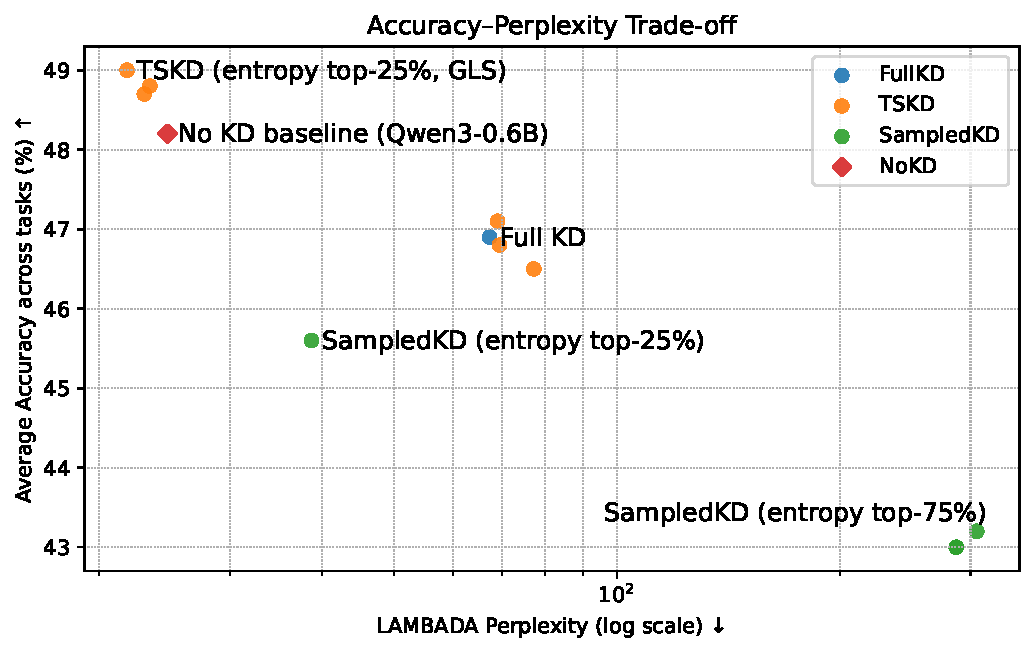
\includegraphics[width=\linewidth]{fig_pareto_acc_vs_ppl.pdf}
\caption{Accuracy--perplexity trade-off across distillation settings. Token-selective KD (TSKD) achieves the best Pareto frontier, while SampledKD compresses storage at a modest accuracy cost.}
\label{fig:acc-ppl}
\end{figure}

Figure~\ref{fig:acc-ppl} highlights the Pareto frontier we observe: SampledKD occupies the low-perplexity, high-efficiency region, whereas TSKD dominates the accuracy axis.
SampledKD achieves large logit-storage reductions ($\sim8k-16k\times$) while maintaining competitive accuracy.
In our small-scale setting it does not yet close the gap to FullKD, but we believe further tuning and scaling could help bridge this gap, since linearity across SampledKD and TSKD is observed.

From training dynamics and ablations we hypothesize four drivers of underperformance in some variants:
(i) Narrow supervision - distillation was applied on a single dataset and only a subset of it, giving the student limited coverage of the teacher's distribution;
(ii) Limited tuning - key hyperparameters (selection thresholds, sampling temperature, loss weights) were not extensively optimized;
(iii) Insufficient scale - the small 0.6B student and 4M-token budget likely did not fully exploit the teacher signal; and
(iv) Evaluation mismatch - zero-shot evaluation may not reflect the distribution the student was trained on.

For SampledKD, training on the GSM8K split yielded stronger numbers than zero-shot, suggesting the weak zero-shot outcomes stem from supervision bias, variance, and scale limits rather than a flaw in the distillation objective.

\section{Related Work}

Foundational KD \citep{hinton2015distillation} and encoder-model distillation (e.g., DistilBERT \citep{sanh2019distilbert}) have been extended to generative LMs, including sequence-level KD for neural machine translation (NMT) \citep{kim2016sequencekd}, student-to-teacher KL distillation (MiniLLM) \citep{gu2023minillm}, and on-policy distillation, where the student generates its own text and learns from the teacher's feedback, to mitigate exposure bias (GKD) \citep{agarwal2024gkd}.
More recently, cross-tokenizer distillation has been enabled by Universal Logit Distillation (ULD) \citep{boizard2024uld} and others.

\subsection{Sparse logit KD and calibration}
Deterministic top-$K$/percentile caching of teacher logits (e.g., SLIM \citep{raman2023slim} and top-$5$ variants) reduces storage but discards tail mass, inducing biased gradients and miscalibrated students.
Random-Sampling KD \citep{anshumann2025sparse} replaces truncation with importance sampling to provide unbiased gradient estimates and improved calibration.
While they have explored orthogonal improvements such as CE--KLD mixing and confidence-based reweighting at the loss level, our work targets token-level selection with different confidence metrics.
Trustworthy distillation (\emph{FIRST}) targets calibration by processing top-$k$ vocabulary tokens with temperature scaling and label smoothing \citep{shum2024first}, whereas we apply entropy/KL-based position selection coupled with RS-KD over classes.

\subsection{Token-/word-level selective supervision} Several strands selectively apply supervision at the granularity we target. In NMT, \citet{wang2021selectivekd} select high cross-entropy \emph{words} using both batch-local and global FIFO queues (GLS). For LLM post-training, token-level uncertainty-aware learning applies masked MLE on high-uncertainty \emph{tokens} and self-distillation on the remainder to avoid OOD overfitting \citep{liu2025tokenlevel}. In continual KD, token-level cross-entropy is used to quantify when and where to distill \citep{zhang2023continualkd}. In CoT reasoning, KPOD learns token importance weights and a progressive schedule within rationales \citep{feng2024kpod}.
Compared to these, TSKD and SampledKD select tokens using teacher-centric uncertainty (entropy and teacher-student KL) and couples selection with unbiased class-level RS-KD at selected positions.

\subsection{Entropy/uncertainty-guided KD} Beyond selection, multiple KD variants weight supervision by uncertainty or entropy.
Entropy-based adaptive KD (EA-KD) prioritizes \emph{samples} with higher entropy \citep{su2023eakd}, while DE-MKD uses teacher-prediction entropy to weight among multiple teachers \citep{cheng2024demkd}.
Uncertainty-aware mixup reduces KD cost while maintaining quality \citep{xu2023unix}.
Recent work also shows entropy-weighted distillation can improve reliability/calibration in classification \citep{guo2024entropykd}.
Our methods differ in using entropy/KL primarily to decide which tokens receive external-teacher KD, not to reweight losses globally.

% (moved) Entropy approximation subsection relocated before Related Work.

\subsection{Entropy/perplexity for data selection} Selecting \emph{samples} by entropy or perplexity is long-standing in NLP.
Moore-Lewis cross-entropy difference and follow-ups established perplexity-based domain selection \citep{moore2010cediff,axelrod2015few,axelrod2017cynical}.
Recent LLM-scale pruning leverages perplexity or loss from small reference models \citep{ankner2024perplexedperplexityperplexitybaseddata} and surveys consolidate techniques \citep{datasel2024survey}.
% Active learning routinely employs entropy/margin sampling \citep{zhang2022alsurvey}. 
Our method is orthogonal: we operate at the token level within sequences and combine selection with unbiased sparse logits.

\section{Limitations and Future Work}
\label{sec:limits}
\paragraph{Scale and quantization}
Our primary teacher-student pair (Qwen3-8B $\rightarrow$ Qwen3-0.6B) and the use of 8-bit quantization during training likely amplify variance in the sampled objectives and partly explain the residual gap we observe for SampledKD.
We expect different behavior at larger teacher/student scales and without low-precision constraints.

\subsection{SampledKD underperformance}
SampledKD is principled and inherits successes from RS-KD, but in our current setting it does not yet match full KD at equal wall-clock.
We attribute the gap to: limited training budget (4M FineWeb-Edu tokens), predominantly zero-shot evaluation, low-precision training, and length filtering of documents above max\_seq\_len=256, which biases the data toward short documents relative to FineWeb-Edu (average length $\approx750$).
FineWeb-Edu also mixes diverse domains, which is a poor match for math-reasoning tasks such as GSM8K, where degradation is most pronounced.

\subsection{Future work}
Other than the said enhancements (larger scale, full precision), we see several additional promising directions to close the gap for SampledKD:
(1) Curriculum learning based KD for stability, where token-entropy schedules gradually increase difficulty;
(2) a short on-policy distillation phase after off-policy SampledKD (e.g., SKD/GKD) to rebalance calibration once accuracy has improved \citep{xu2024speculative}.

From a computational perspective, each student distillation step in TSKD still requires a full softmax and significant runtime, for both the KLD and CE.
SampledKD, while reducing the computational overhead of each KLD, still does not eliminate the need for full-vocabulary softmax at the CE level, and additionally requires at least 1 full vocabulary pass for the KLD at both the student and the teacher.
We have explored softmax approximation techniques, but they did not yield satisfactory accuracy.

Similarly to GLS, normalizing selection tokens count in document lengths is another promising direction to explore in order to mitigate the influence of specific batch properties (e.g., length, averaged entropy) on the selection process.

\section{Conclusion}
\label{sec:conclusion}
We introduced TSKD and SampledKD, which augments token selection with class-level RS-KD.
TSKD provides stronger efficiency-accuracy trade-offs than FullKD on several benchmarks in our setting.
SampledKD yields far larger logit-storage reductions with competitive accuracy, but in our small-scale, low-precision setting still lags behind the FullKD (and understandably behind TSKD).
Given its unbiased foundations and the prior success of RS-KD, we expect SampledKD to become more impactful at larger scales.

\bibliography{custom}
\bibliographystyle{acl_natbib}

\appendix
\section{Training Hyperparameters}
\label{app:hyperparams}

Tables~\ref{tab:shared-hparams} and~\ref{tab:variant-hparams} list the hyperparameter choices shared across all runs and the settings that differ between distillation variants.

\begin{table}[h]
	\centering
	\small
	\setlength{\tabcolsep}{8pt}
\begin{tabular}{p{0.25\linewidth}p{0.65\linewidth}}
Component & Value \\
\midrule
Teacher model & Qwen/Qwen3-8B (8-bit quantized) \\
Student model & Qwen/Qwen3-0.6B with gradient checkpointing \\
Dataset & FineWeb-Edu stream capped at 4M tokens \\
Sequence cap & 256 tokens (implemented as \texttt{max\_seq\_len=250}) \\
Epochs & 1 pass over the streamed subset \\
Mini-batch & 1 sample \(\times 32\) gradient steps (effective batch 32) \\
Optimizer & bitsandbytes Adam8bit (lr $1\times 10^{-5}$; AdamW fallback) \\
KD temperature & 2.0 (no annealing) \\
CE mixing weight & $\alpha_{\text{CE}}=0.3$ with KD always on ($1-\alpha_{\text{CE}}$) \\
Offline cache & Enabled with $U=12$ cached classes and uint8 $\hat H$ \\
Entropy approx. & Top-$m$ with m=12; rs\_vocab\_samples=12 \\
Seed & 1337 (deterministic off) \\
\bottomrule
\end{tabular}
\caption{Shared hyperparameters across all experiments.}
\label{tab:shared-hparams}
\end{table}

\begin{table}[h]
	\centering
	\small
	\setlength{\tabcolsep}{8pt}
\begin{tabular}{p{0.32\linewidth}p{0.6\linewidth}}
Variant & Additional settings \\
\midrule
Full KD & Distills all tokens; offline cache used only for entropy logging (no subsampling). \\
TSKD (entropy top-$k$) & $k\in\{20,25,75\}$; GLS queue size $30\,000$ tokens when enabled; no composite score unless stated. \\
TSKD (bucket) & Bucket range $(75,95)$ when active. \\
Random / Pos-RS-KD token selection & Same $k$ values as entropy top-$k$ with $\alpha=1.0$, $\epsilon=0.02$, $q_{\min}=10^{-6}$. \\
LinUCB selector & $\alpha=1.0$, $\lambda=1.0$, reward clip $\pm 5$. \\
\bottomrule
\end{tabular}
\caption{Settings specific to each distillation variant reported in the main tables.}
\label{tab:variant-hparams}
\end{table}

\section{Positional RS-KD matches the equal-weight KD objective}
\label{app:pos-rs-kd-proof}

Let \(P_x\) be the set of valid next-token positions for sequence \(x\), and define \(N=\lvert P_x\rvert\).
The target objective of knowledge distillation is
\[
	\mathcal{L}_{\text{KD}}
	=\mathbb{E}_{x}\!\left[\frac{1}{N}\sum_{t\in P_x}\mathrm{KL}(p_t\|s_t)\right].
\]

Let \(q_{\text{pos}}(\cdot)\) be any distribution over \(P_x\) (built from entropies / scores).
Draw \(K_{\text{pos}}\) i.i.d. samples \(t_k\sim q_{\text{pos}}\) (with replacement) and define
\[
	\widehat{\mathcal{L}}_{\text{KD}}^{\text{pos}}(x)
	=\frac{1}{N}\cdot\frac{1}{K_{\text{pos}}}\sum_{k=1}^{K_{\text{pos}}}
	\frac{1}{q_{\text{pos}}(t_k)}\,\mathrm{KL}(p_{t_k}\|s_{t_k}).
\]
Note that the random term can be written as
\[
	\mathrm{KL}(p_{t_k}\|s_{t_k})
	=\sum_{t\in P_x}\mathbf{1}\!\{t_k=t\}\,\mathrm{KL}(p_t\|s_t),
\]
so:
\[
	\mathbb{E}_{t_k\sim q_{\text{pos}}}\!\left[
		\frac{\mathrm{KL}(p_{t_k}\|s_{t_k})}{q_{\text{pos}}(t_k)}
		\right]
	= \sum_{t\in P_x} q_{\text{pos}}(t)\,
	\frac{\mathrm{KL}(p_t\|s_t)}{q_{\text{pos}}(t)}.
\]
And taking \(\mathbb{E}_x\) over dataset distribution of \(x\) yields \(\mathcal{L}_{\text{KD}}\):
\begin{align*}
	\mathbb{E}\!\left[\widehat{\mathcal{L}}_{\text{KD}}^{\text{pos}}(x)\right]
	 & = \frac{1}{N K_{\text{pos}}}\sum_{k=1}^{K_{\text{pos}}}
	\mathbb{E}_{t_k\sim q_{\text{pos}}}\!\left[
		\frac{\mathrm{KL}(p_{t_k}\|s_{t_k})}{q_{\text{pos}}(t_k)}
	\right]                                                    \\
	 & = \frac{1}{N K_{\text{pos}}}\sum_{k=1}^{K_{\text{pos}}}
	\sum_{t\in P_x}\mathrm{KL}(p_t\|s_t)                       \\
	 & = \frac{1}{N}\sum_{t\in P_x}\mathrm{KL}(p_t\|s_t)       \\
	 & =\mathcal{L}_{\text{KD}}.
\end{align*}

\section{Alternative tail estimators (unbiased IS and control variated)}
\label{app:tail-IS}
Let \(T\) denote the \emph{tail index set}, i.e., the set of vocabulary indices lying outside the top-\(m\) logits.
Define the total tail probability mass $P_T=\sum_{v\in T}p_v$, and $q(v)=p_v/P_T$ the tail-normalized sampling distribution. The exact tail contribution to entropy is
\[
	H_T \;=\; -\sum_{v\in T} p_v \log p_v \;=\; -P_T\,\underset{v\sim q}{\mathbb{E}}\,[\log p_v].
\]
\paragraph{Top-$m$ + naive IS} With $s$ samples $v_i\!\sim q$,
\[
	\widehat{H}_T^{\text{IS}}
	= -P_T \cdot \frac{1}{s}\sum_{i=1}^s \log p_{v_i}.
\]
\paragraph{Top-$m$ + control-variated IS (uniform baseline)}
Decompose with the uniform tail $u=\tfrac{P_T}{V-m}$:
\begin{align*}
	\sum_{v\in T} p_v \log p_v
	 & = -P_T\log\!\frac{P_T}{V-m}                                              \\
	 & + P_T\,\underset{v\sim q}{\mathbb{E}}\!\left[\log\!\frac{p_v}{u}\right].
\end{align*}
Thus, the entropy tail is
\[
	H_T^{\text{CV-IS}}
	= \underbrace{-P_T\log\!\frac{P_T}{V-m}}_{\text{baseline}}
	\;-\; P_T \cdot \underset{v\sim q}{\mathbb{E}}\!\left[\log\!\frac{p_v}{u}\right].
\]
With unbiased estimator (using $s$ samples):
\begin{align*}
	\widehat{H}_T^{\text{CV-IS}}
	 & = -P_T\log\!\frac{P_T}{V-m}                                                \\
	 & \quad - P_T \cdot \frac{1}{s}\sum_{i=1}^s \Big(\log p_{v_i} - \log u\Big).
\end{align*}
In all cases, the head contribution $H_{\text{head}}=-\sum_{j\le m}p_{(j)}\log p_{(j)}$ is computed exactly; the final estimate is $H=H_{\text{head}}+\widehat{H}_T$.

\end{document}
